% Bend - L-BFGS-B
\begin{table}[H]
    \centering
    \vspace*{-2.5cm}
    \hspace*{-3cm}
    \begin{tabular}{|c|c|c|c|}
    \hline 
    \emph{Seed} & Opt. continua & Opt. discreta &  Opt. de fabricación \\
    \hline
      \multirow{2}{*}{128} &
      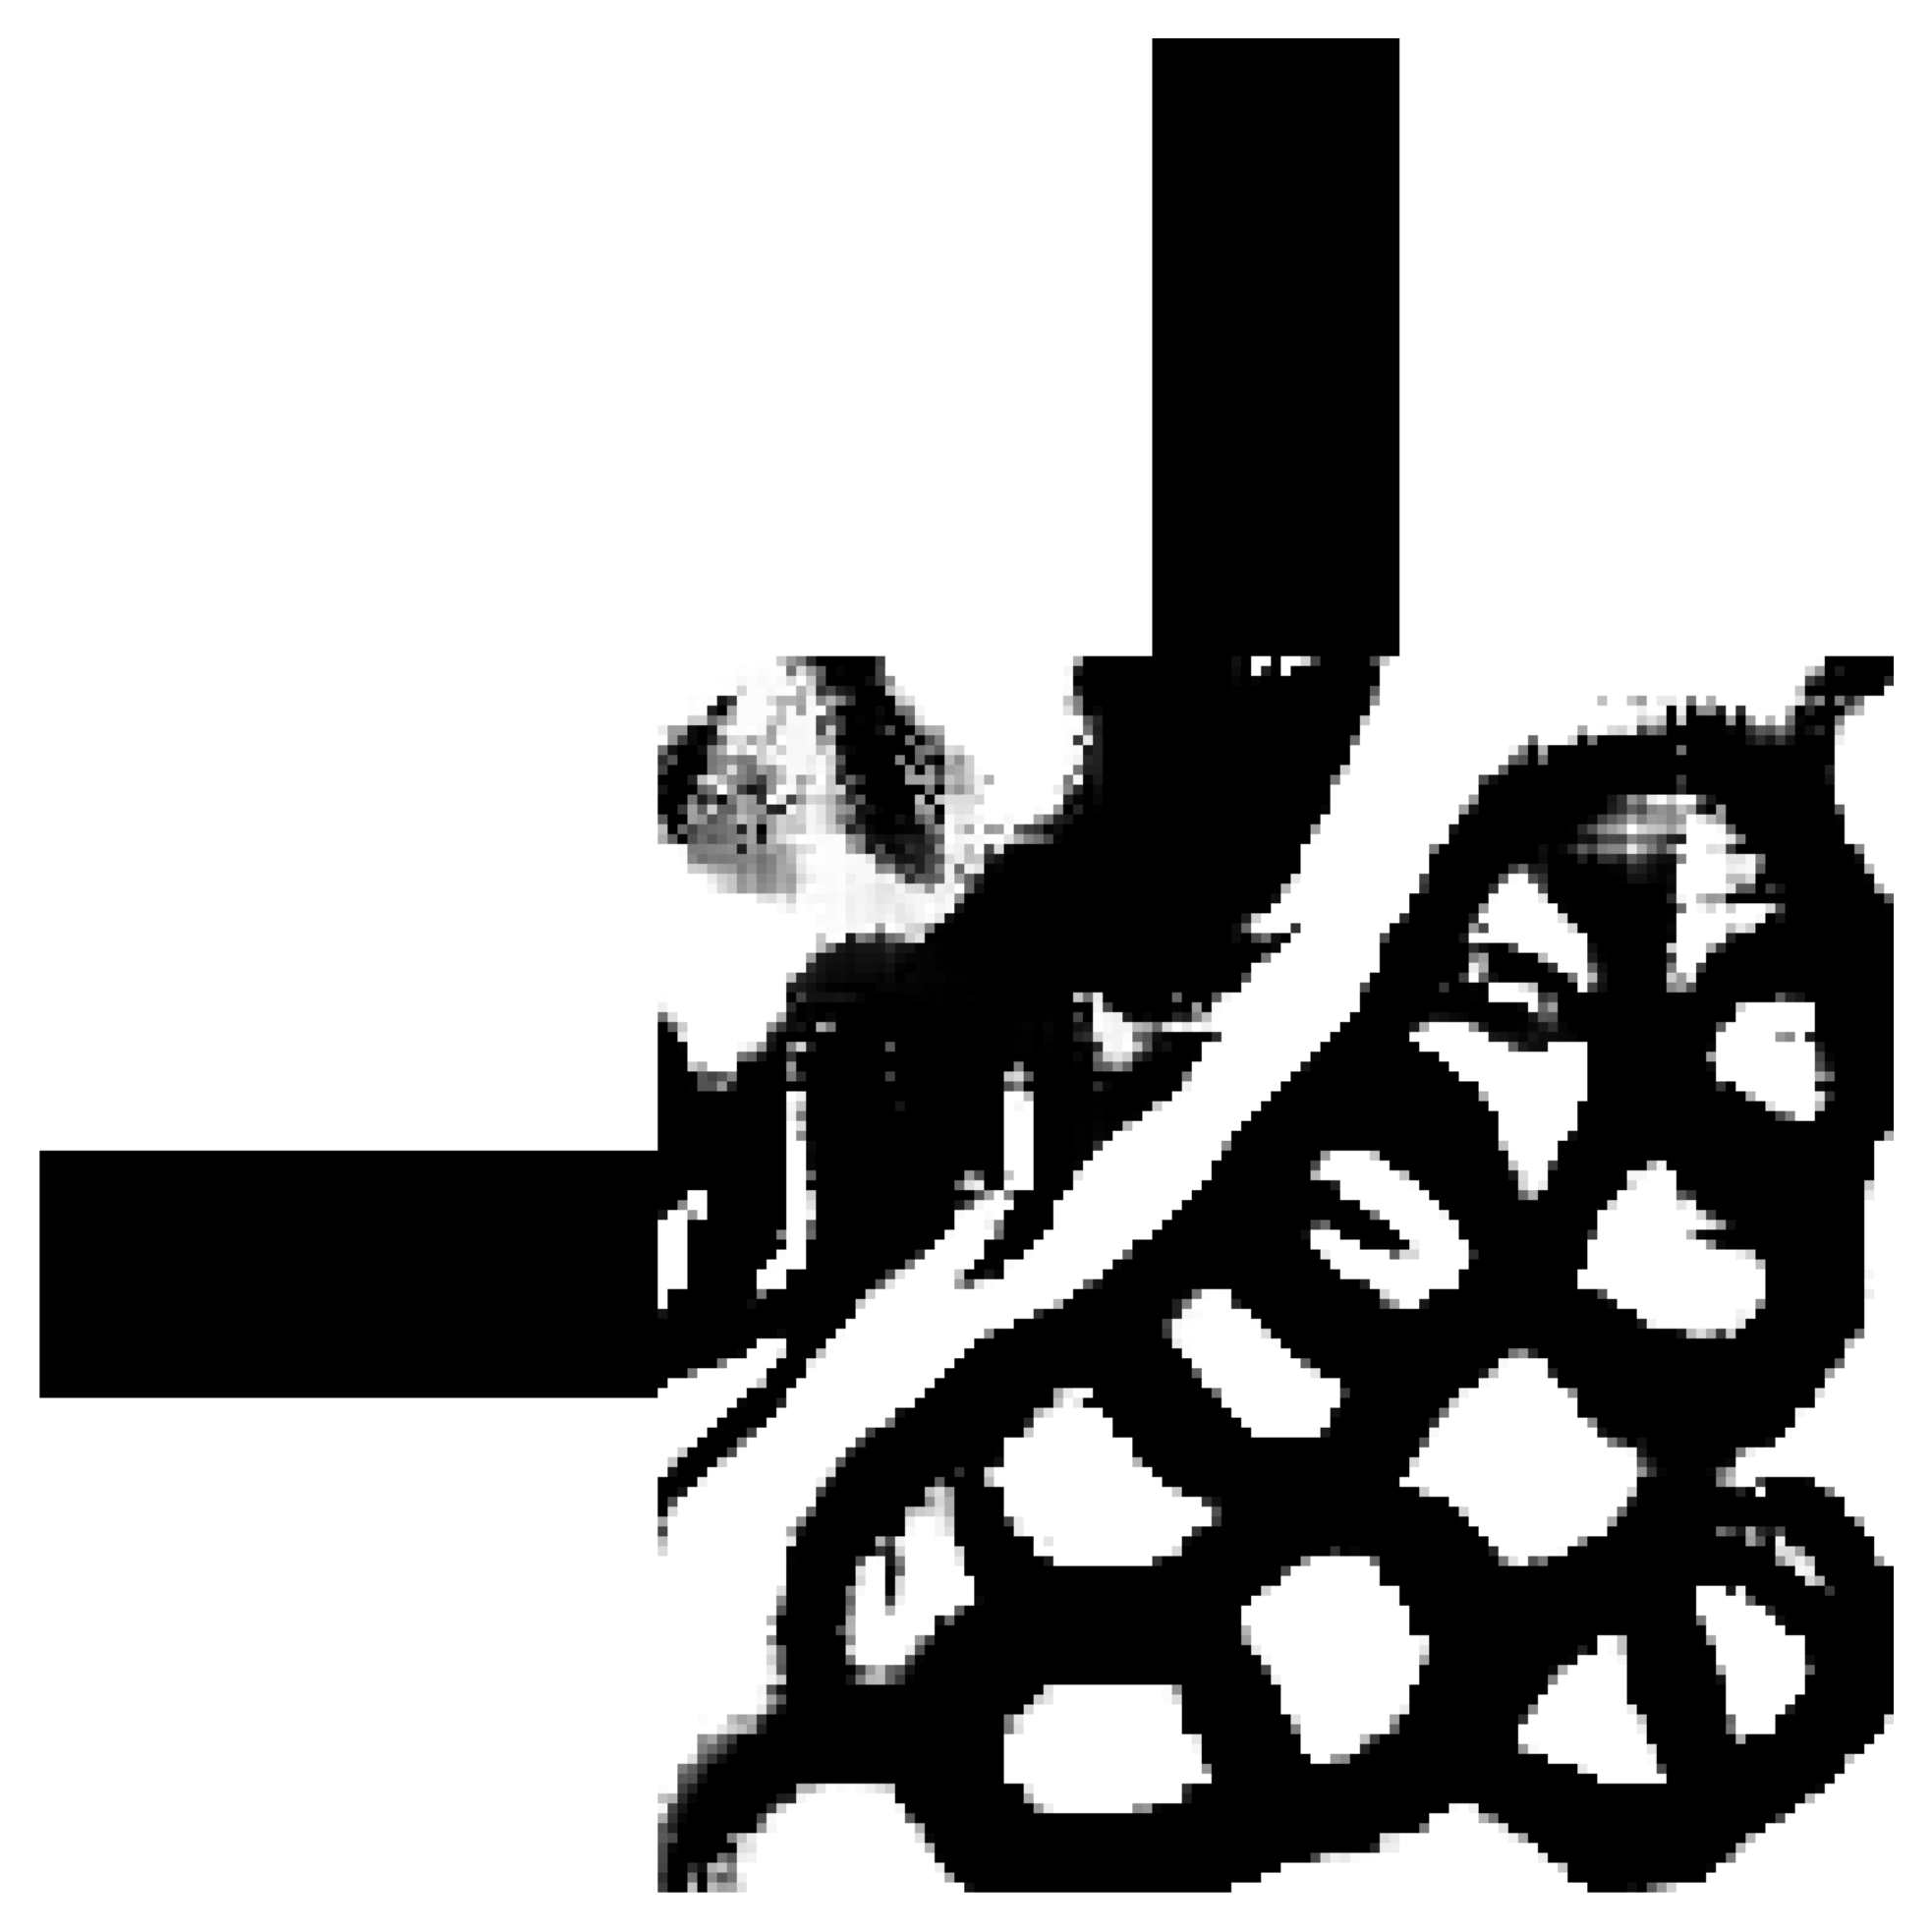
\includegraphics[width=0.20\textwidth]{image/results/bend/L-BFGS-B/visualize_eps_cont_128.png} &
      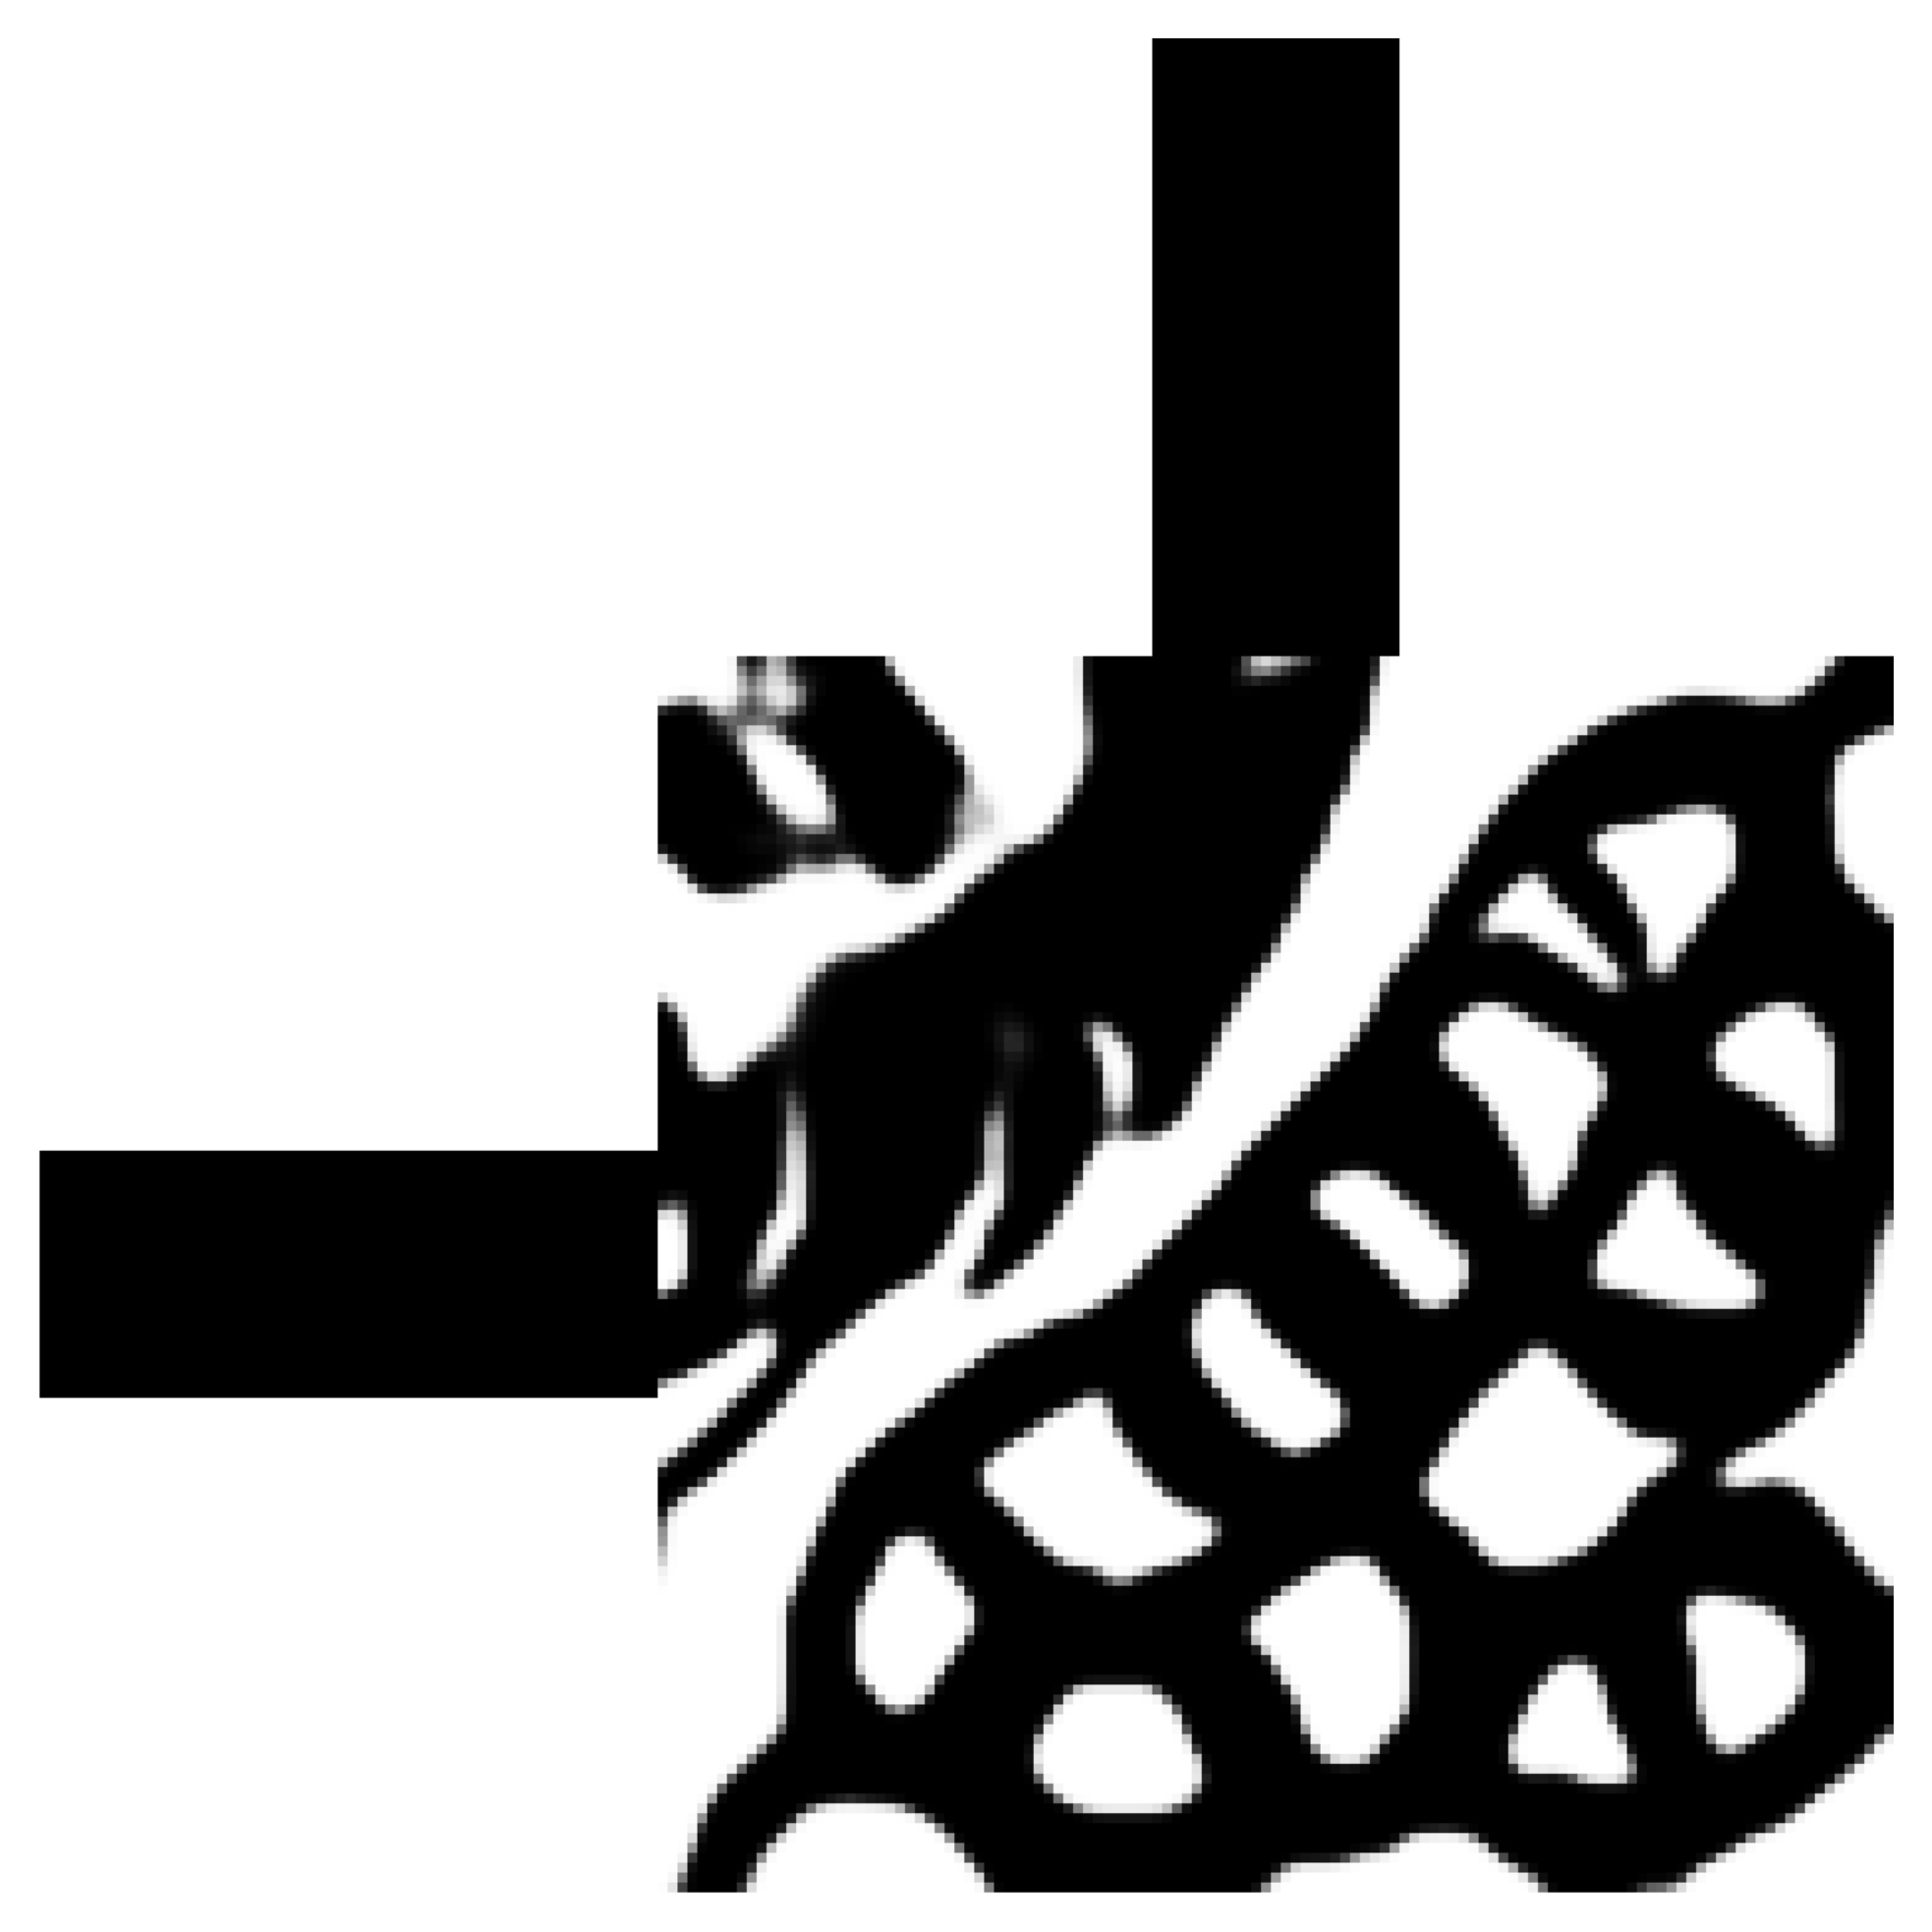
\includegraphics[width=0.20\textwidth]{image/results/bend/L-BFGS-B/visualize_eps_disc_128.png} &
      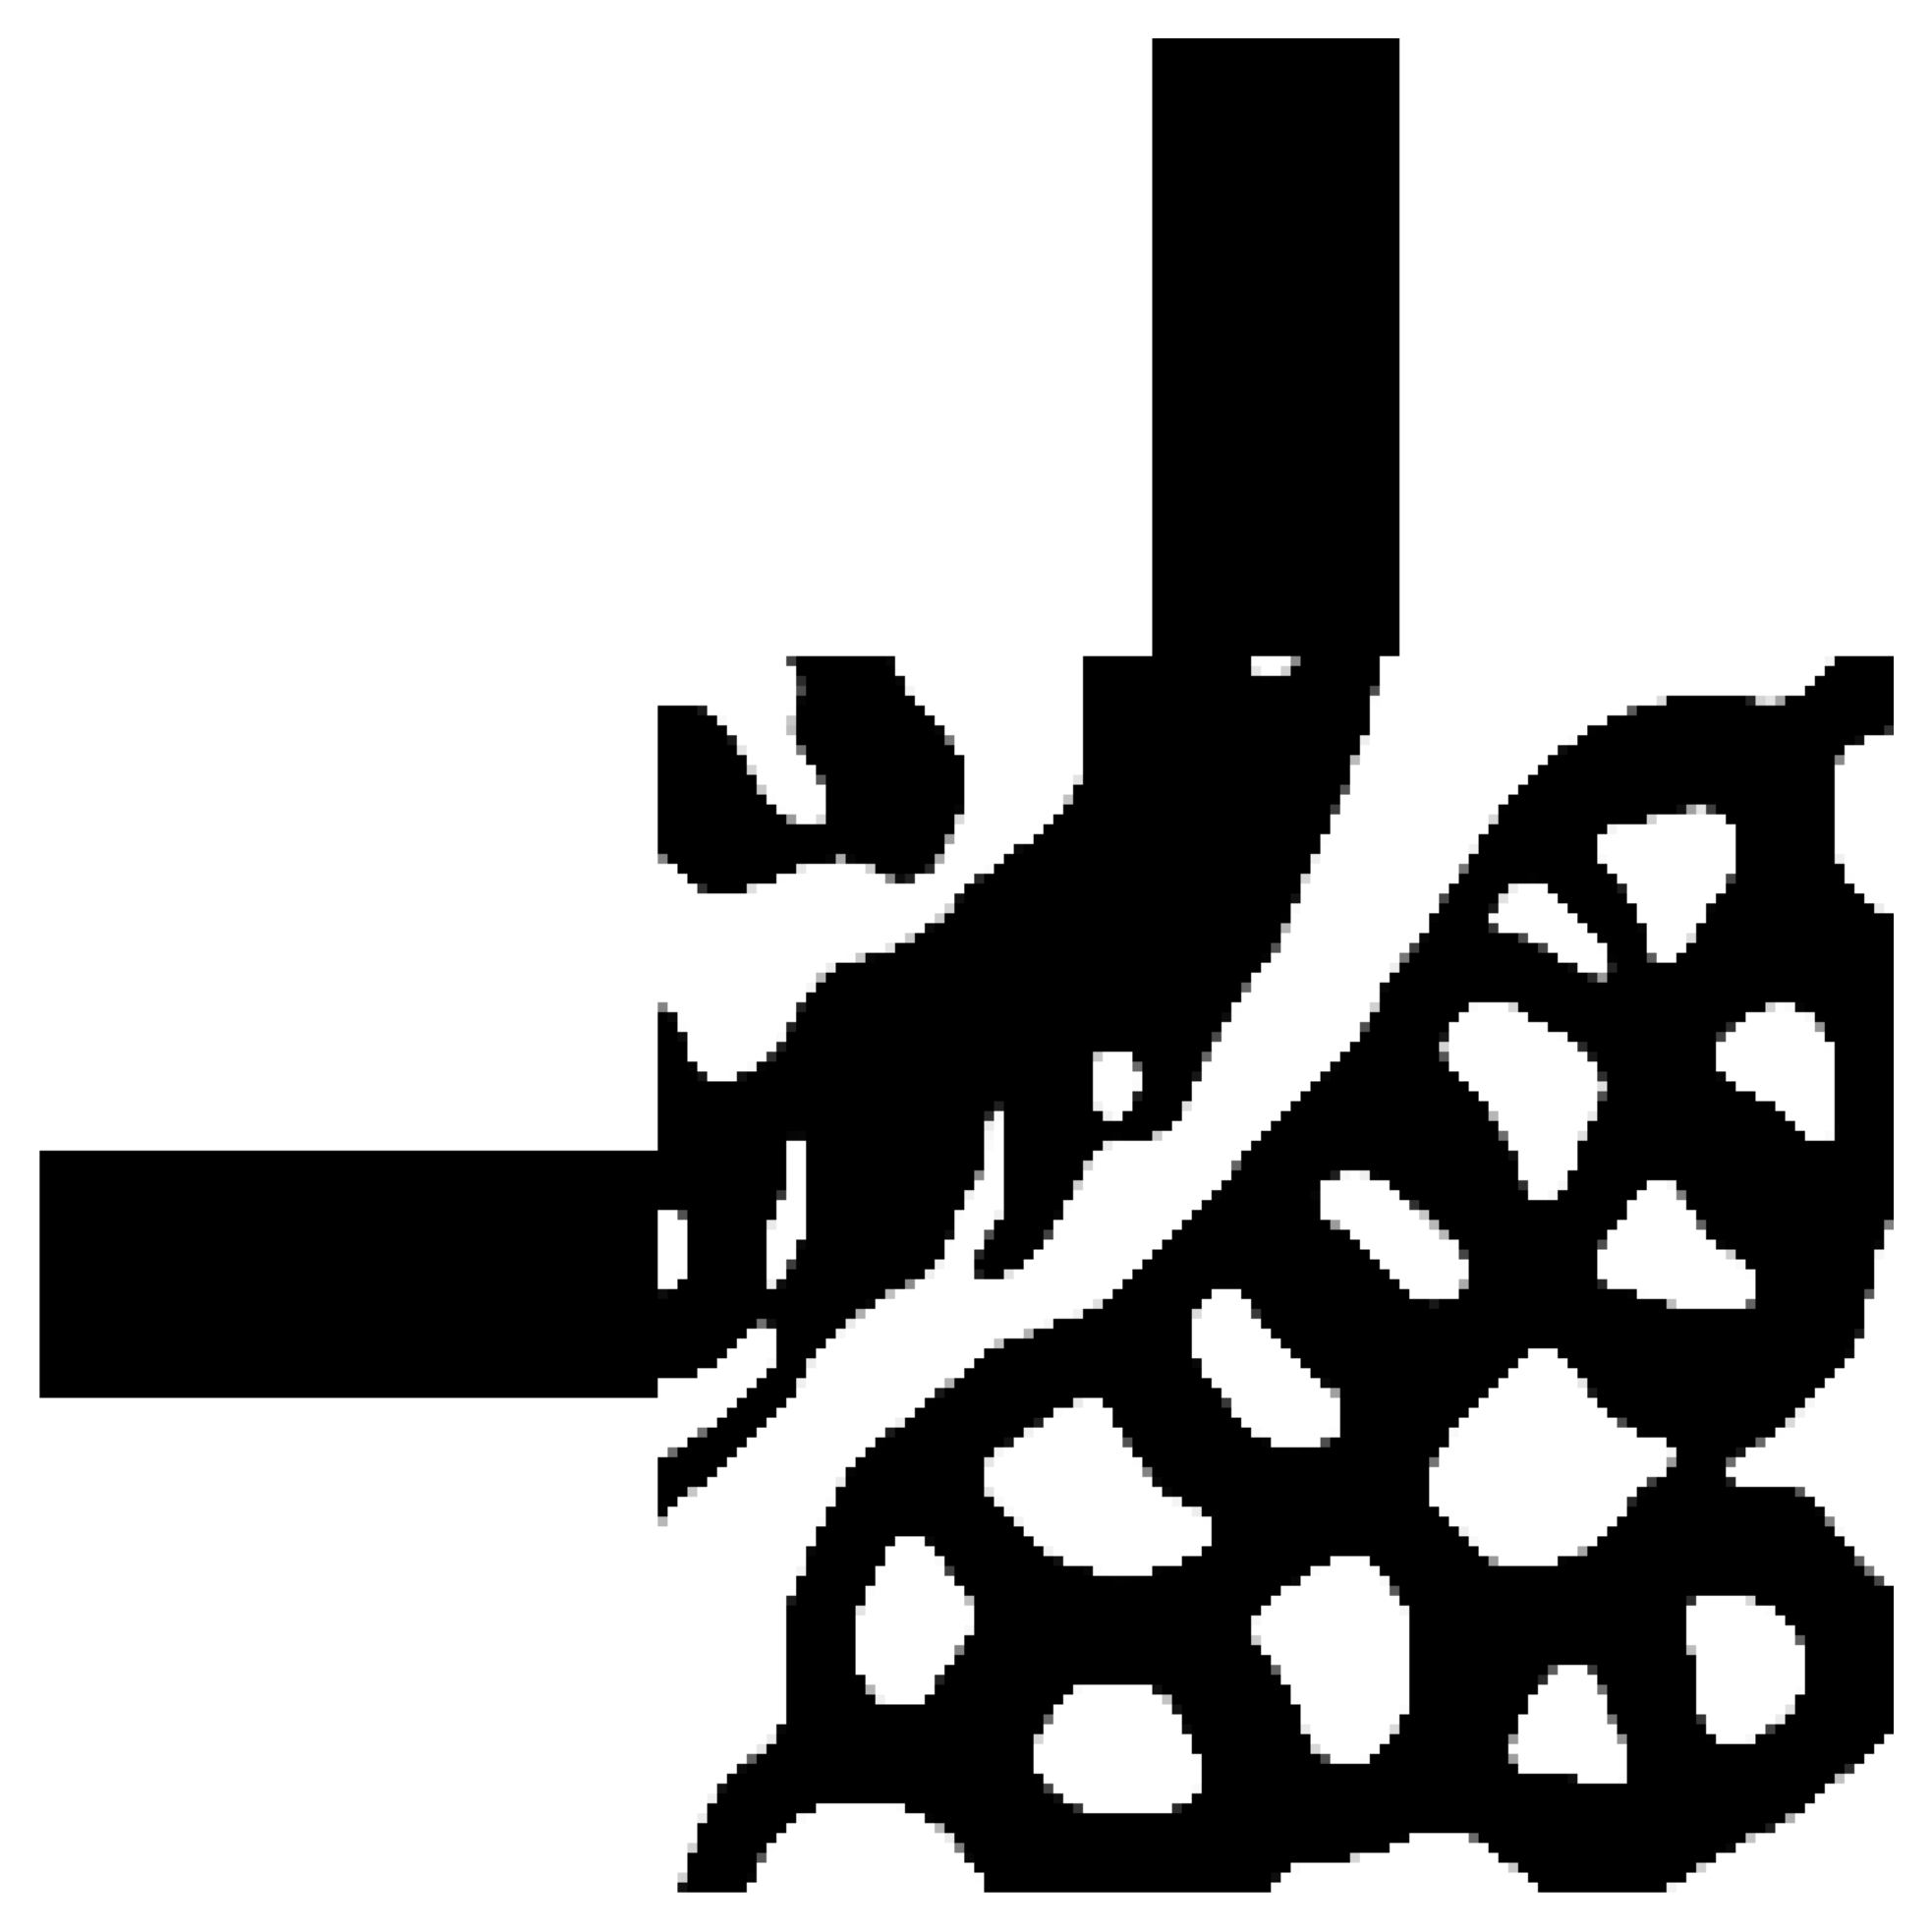
\includegraphics[width=0.20\textwidth]{image/results/bend/L-BFGS-B/visualize_eps_fab_128.png} \\
      \cline{2-4}
      &
      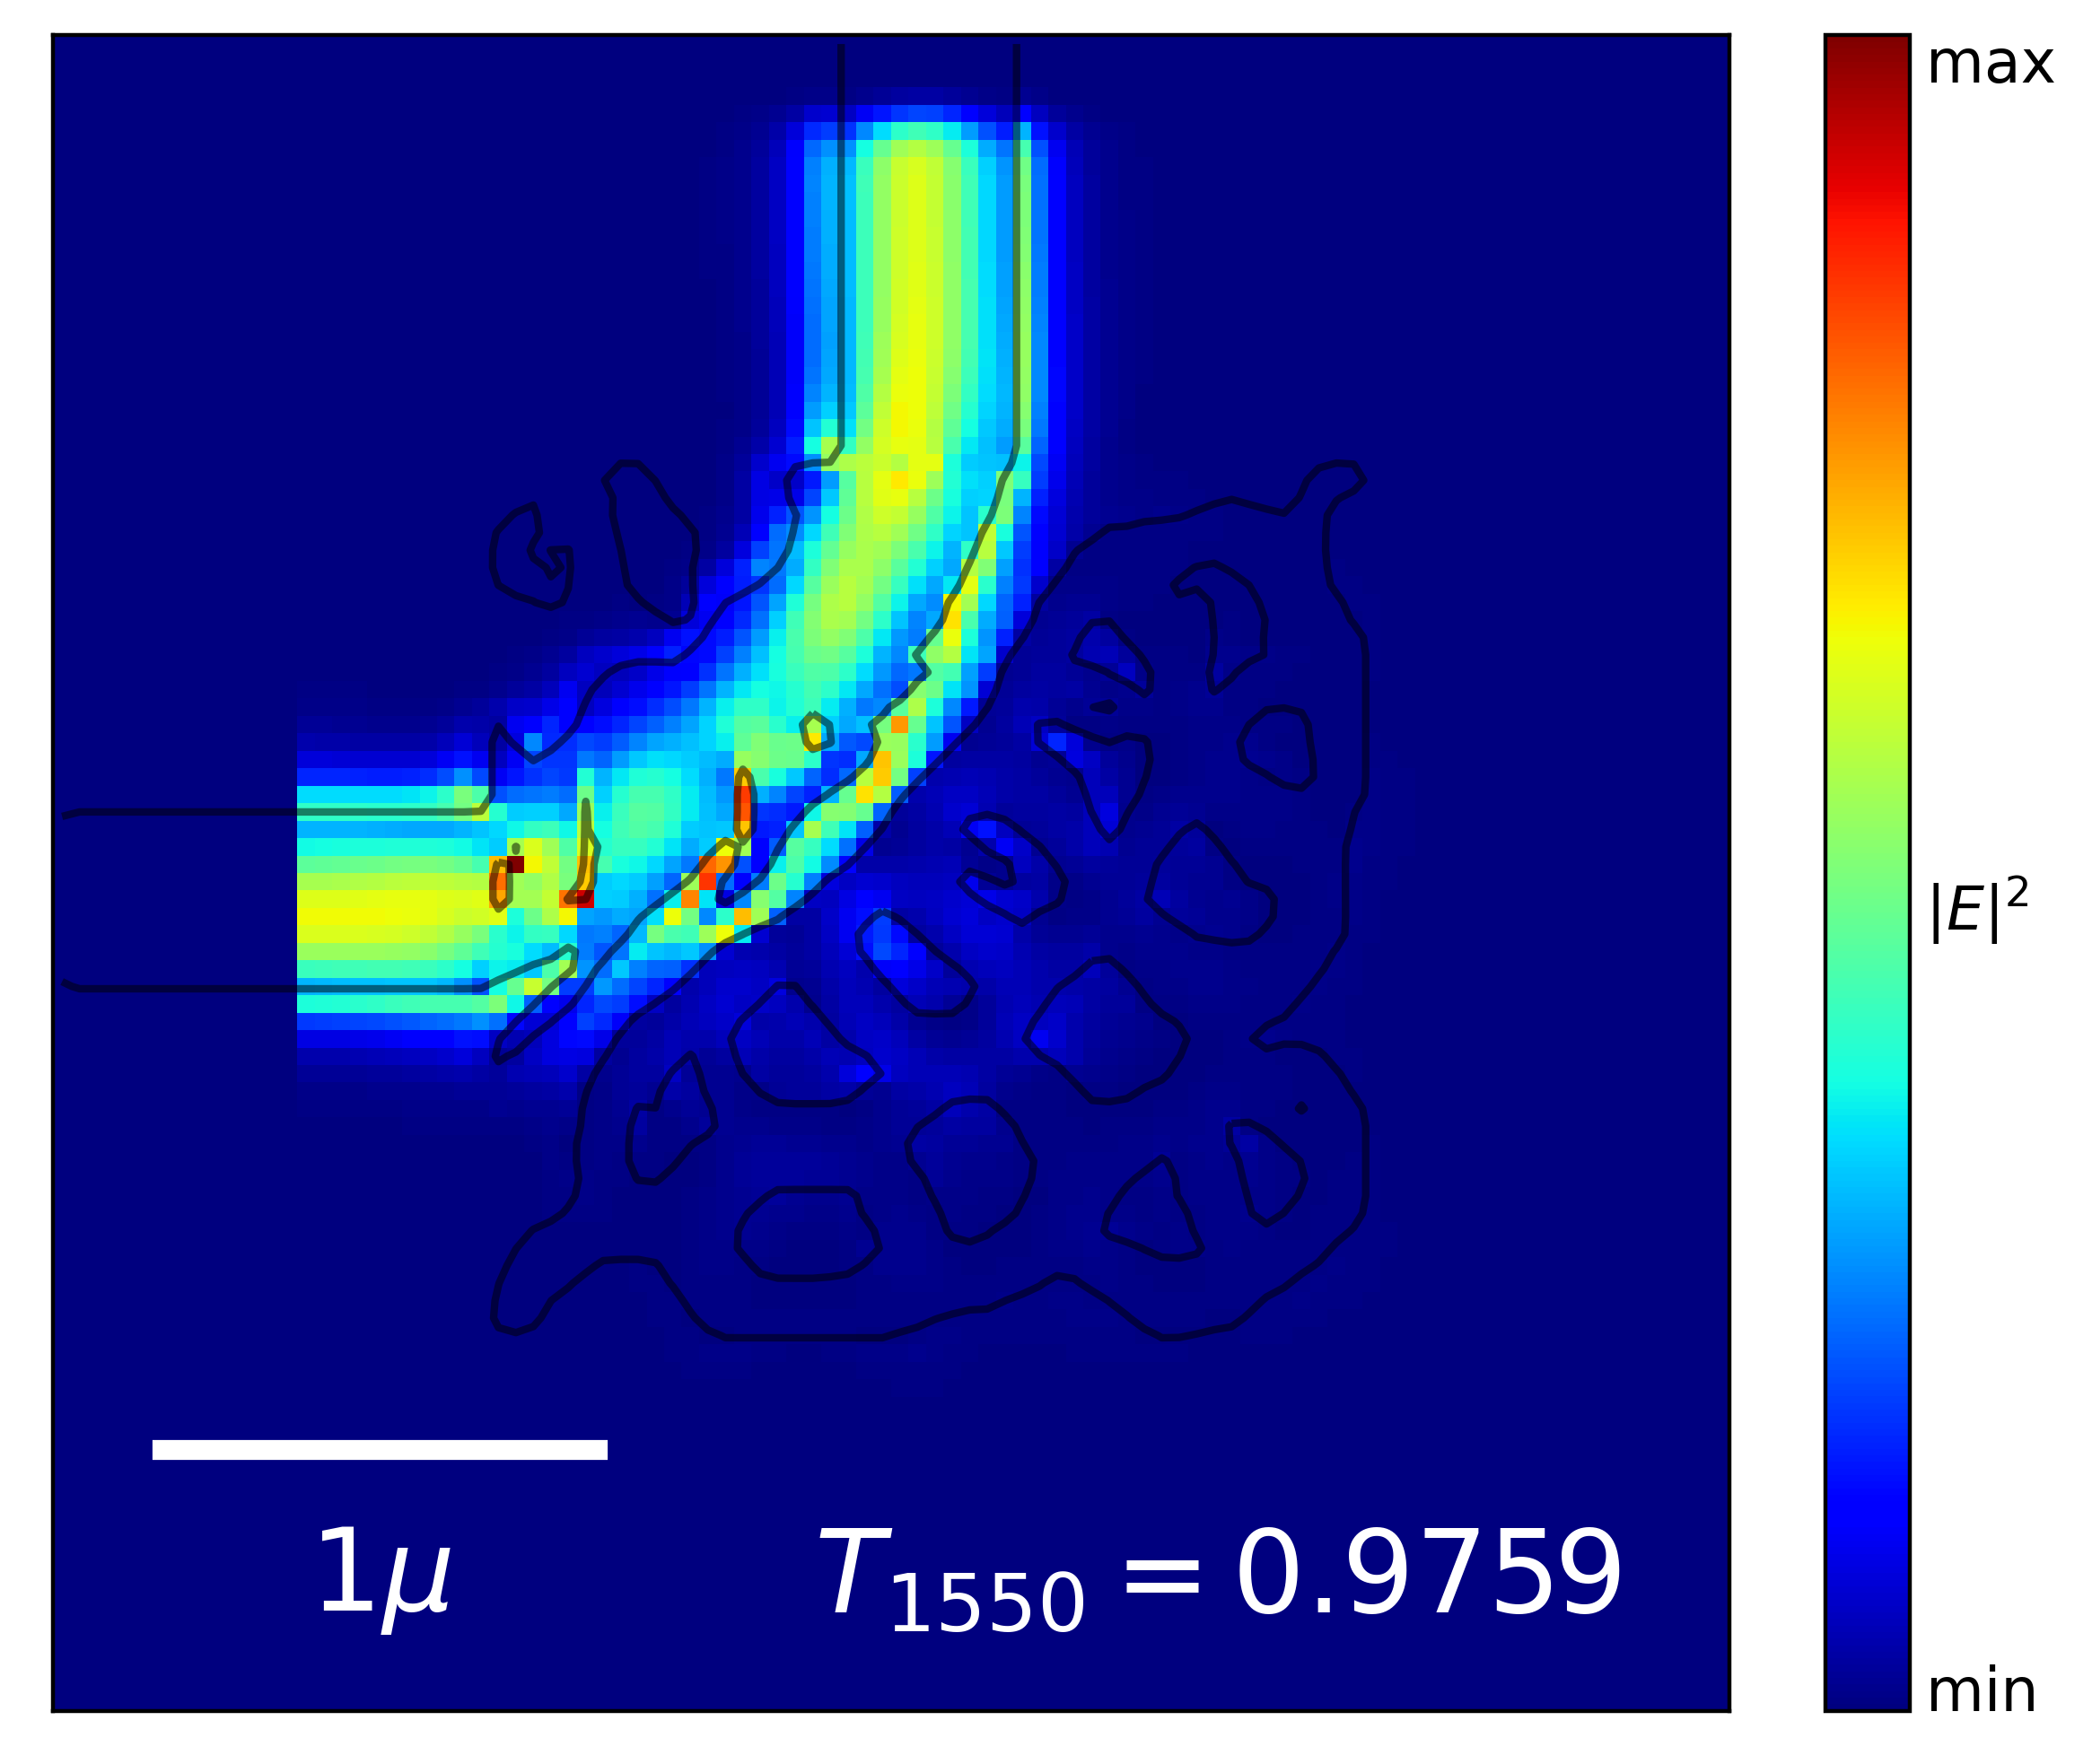
\includegraphics[width=0.33\textwidth]{image/results/bend/L-BFGS-B/visualize_field_cont_128.png} &
      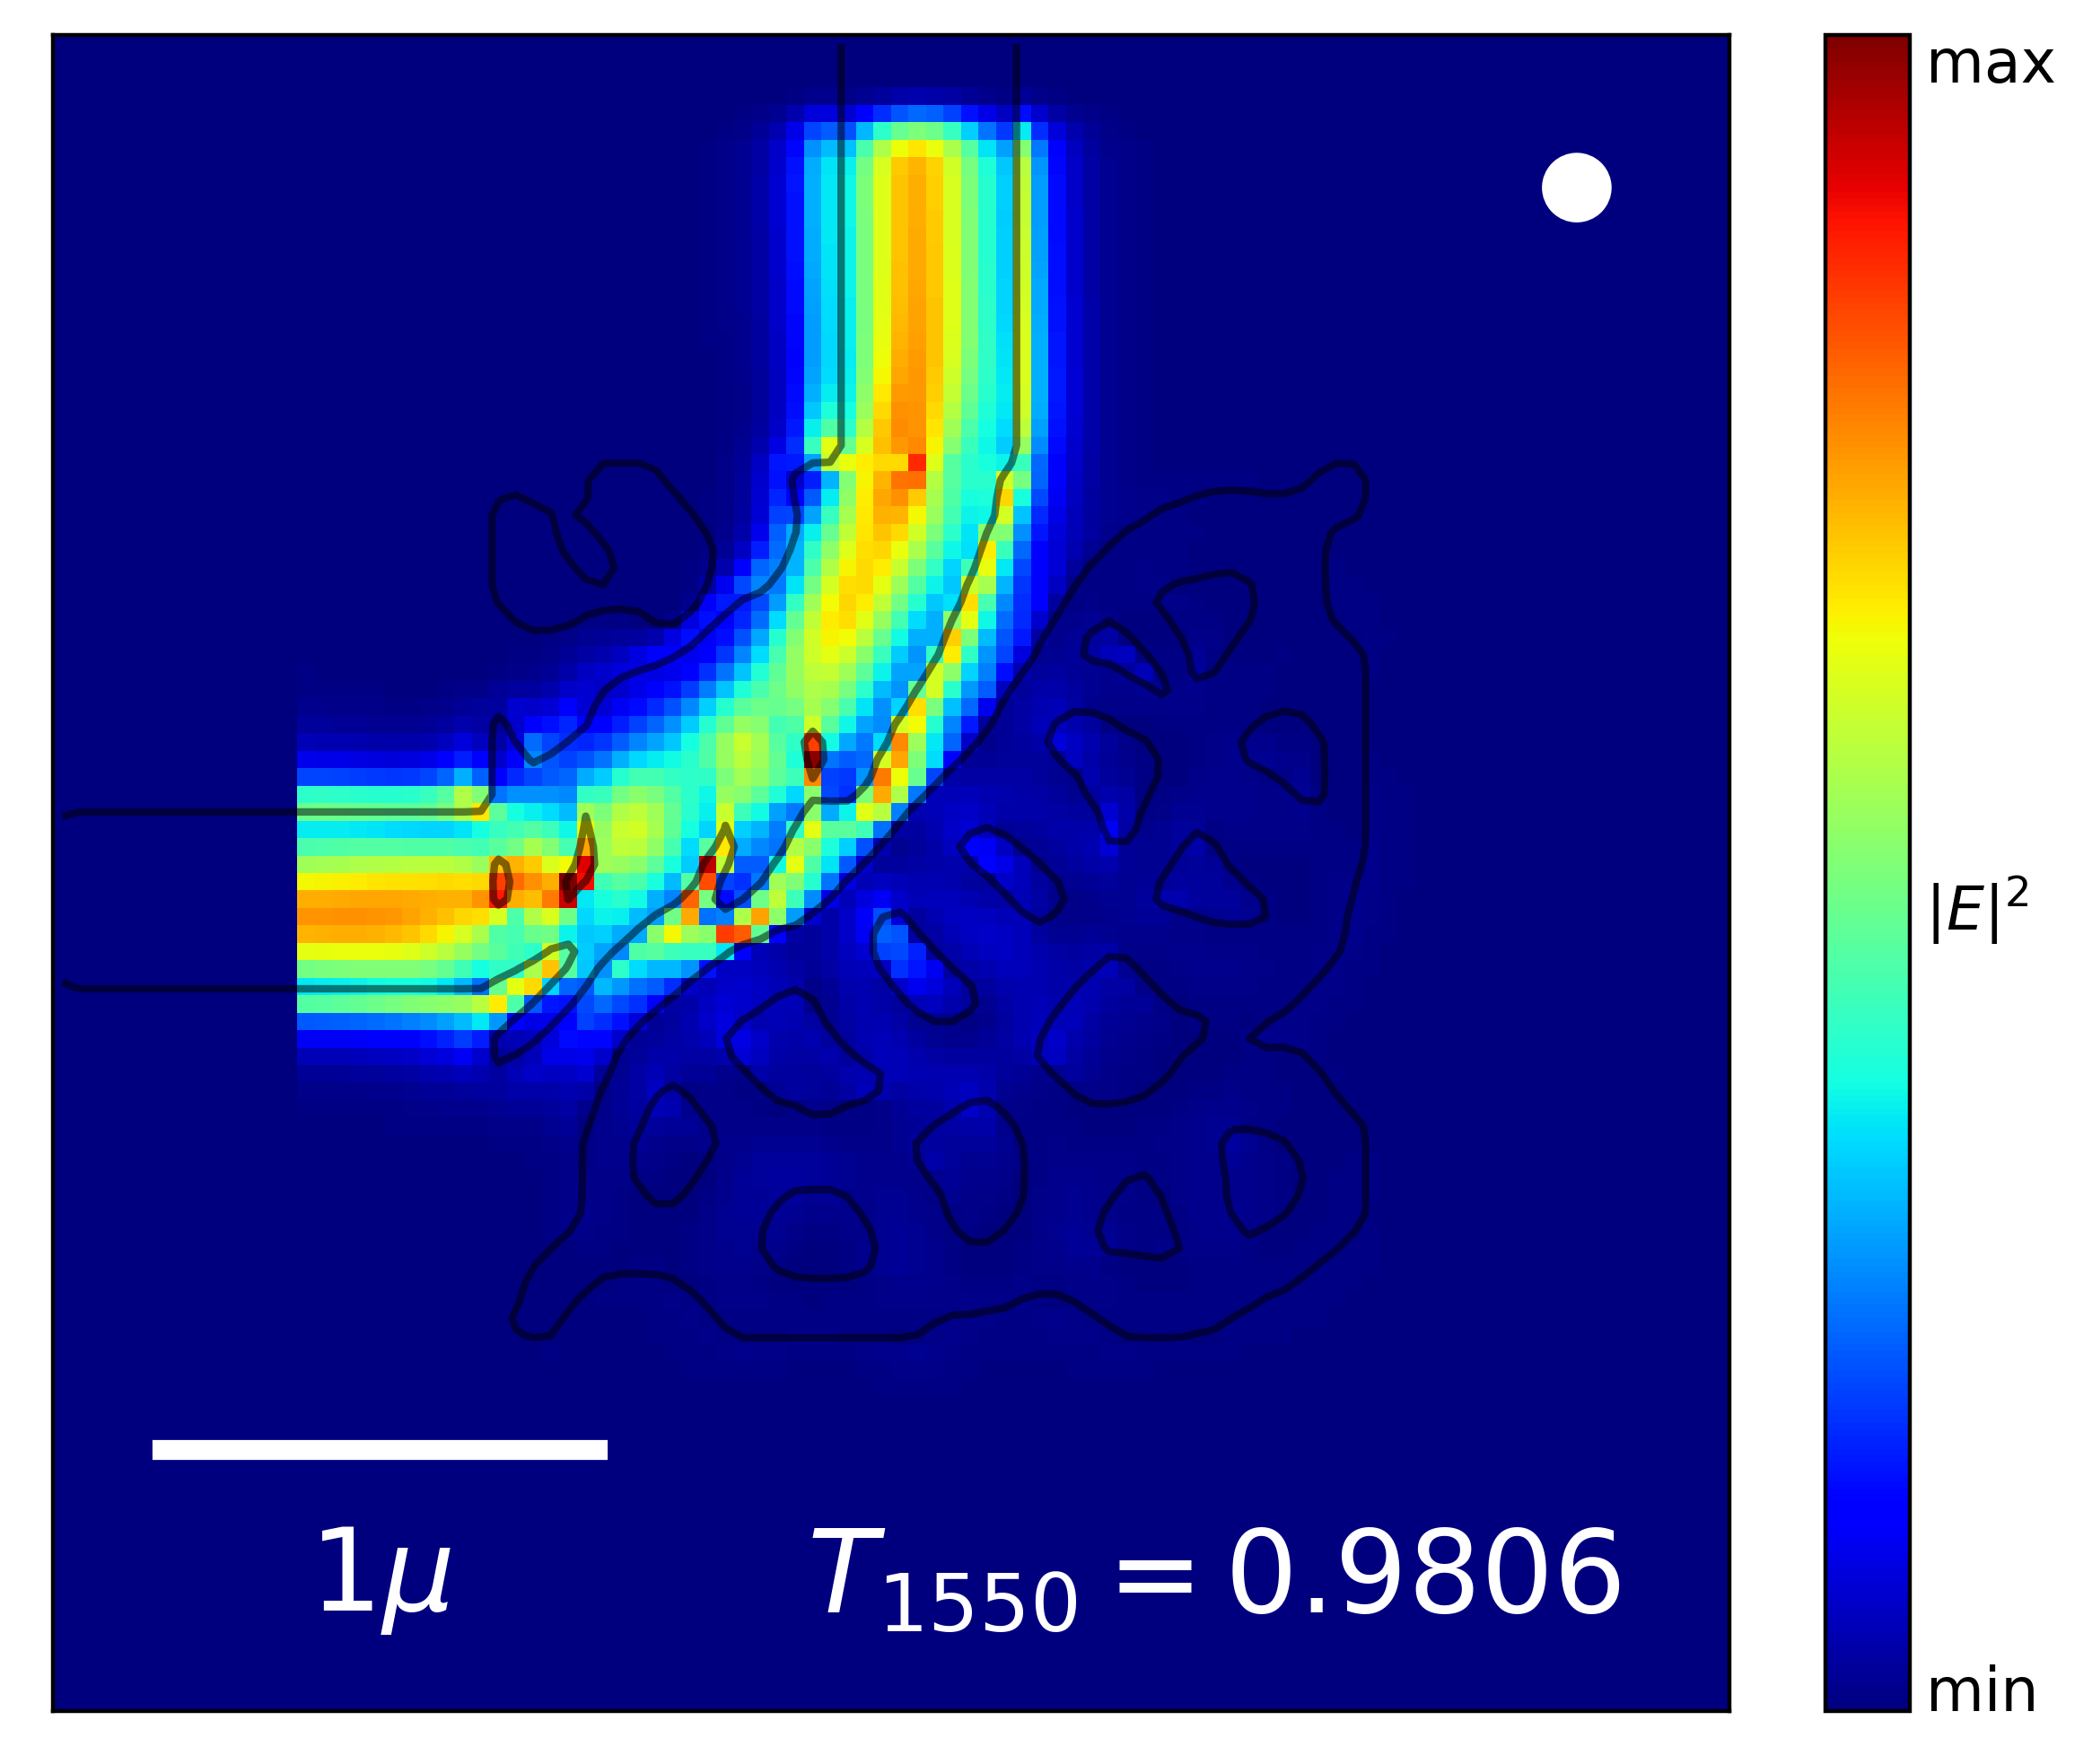
\includegraphics[width=0.33\textwidth]{image/results/bend/L-BFGS-B/visualize_field_disc_128.png} &
      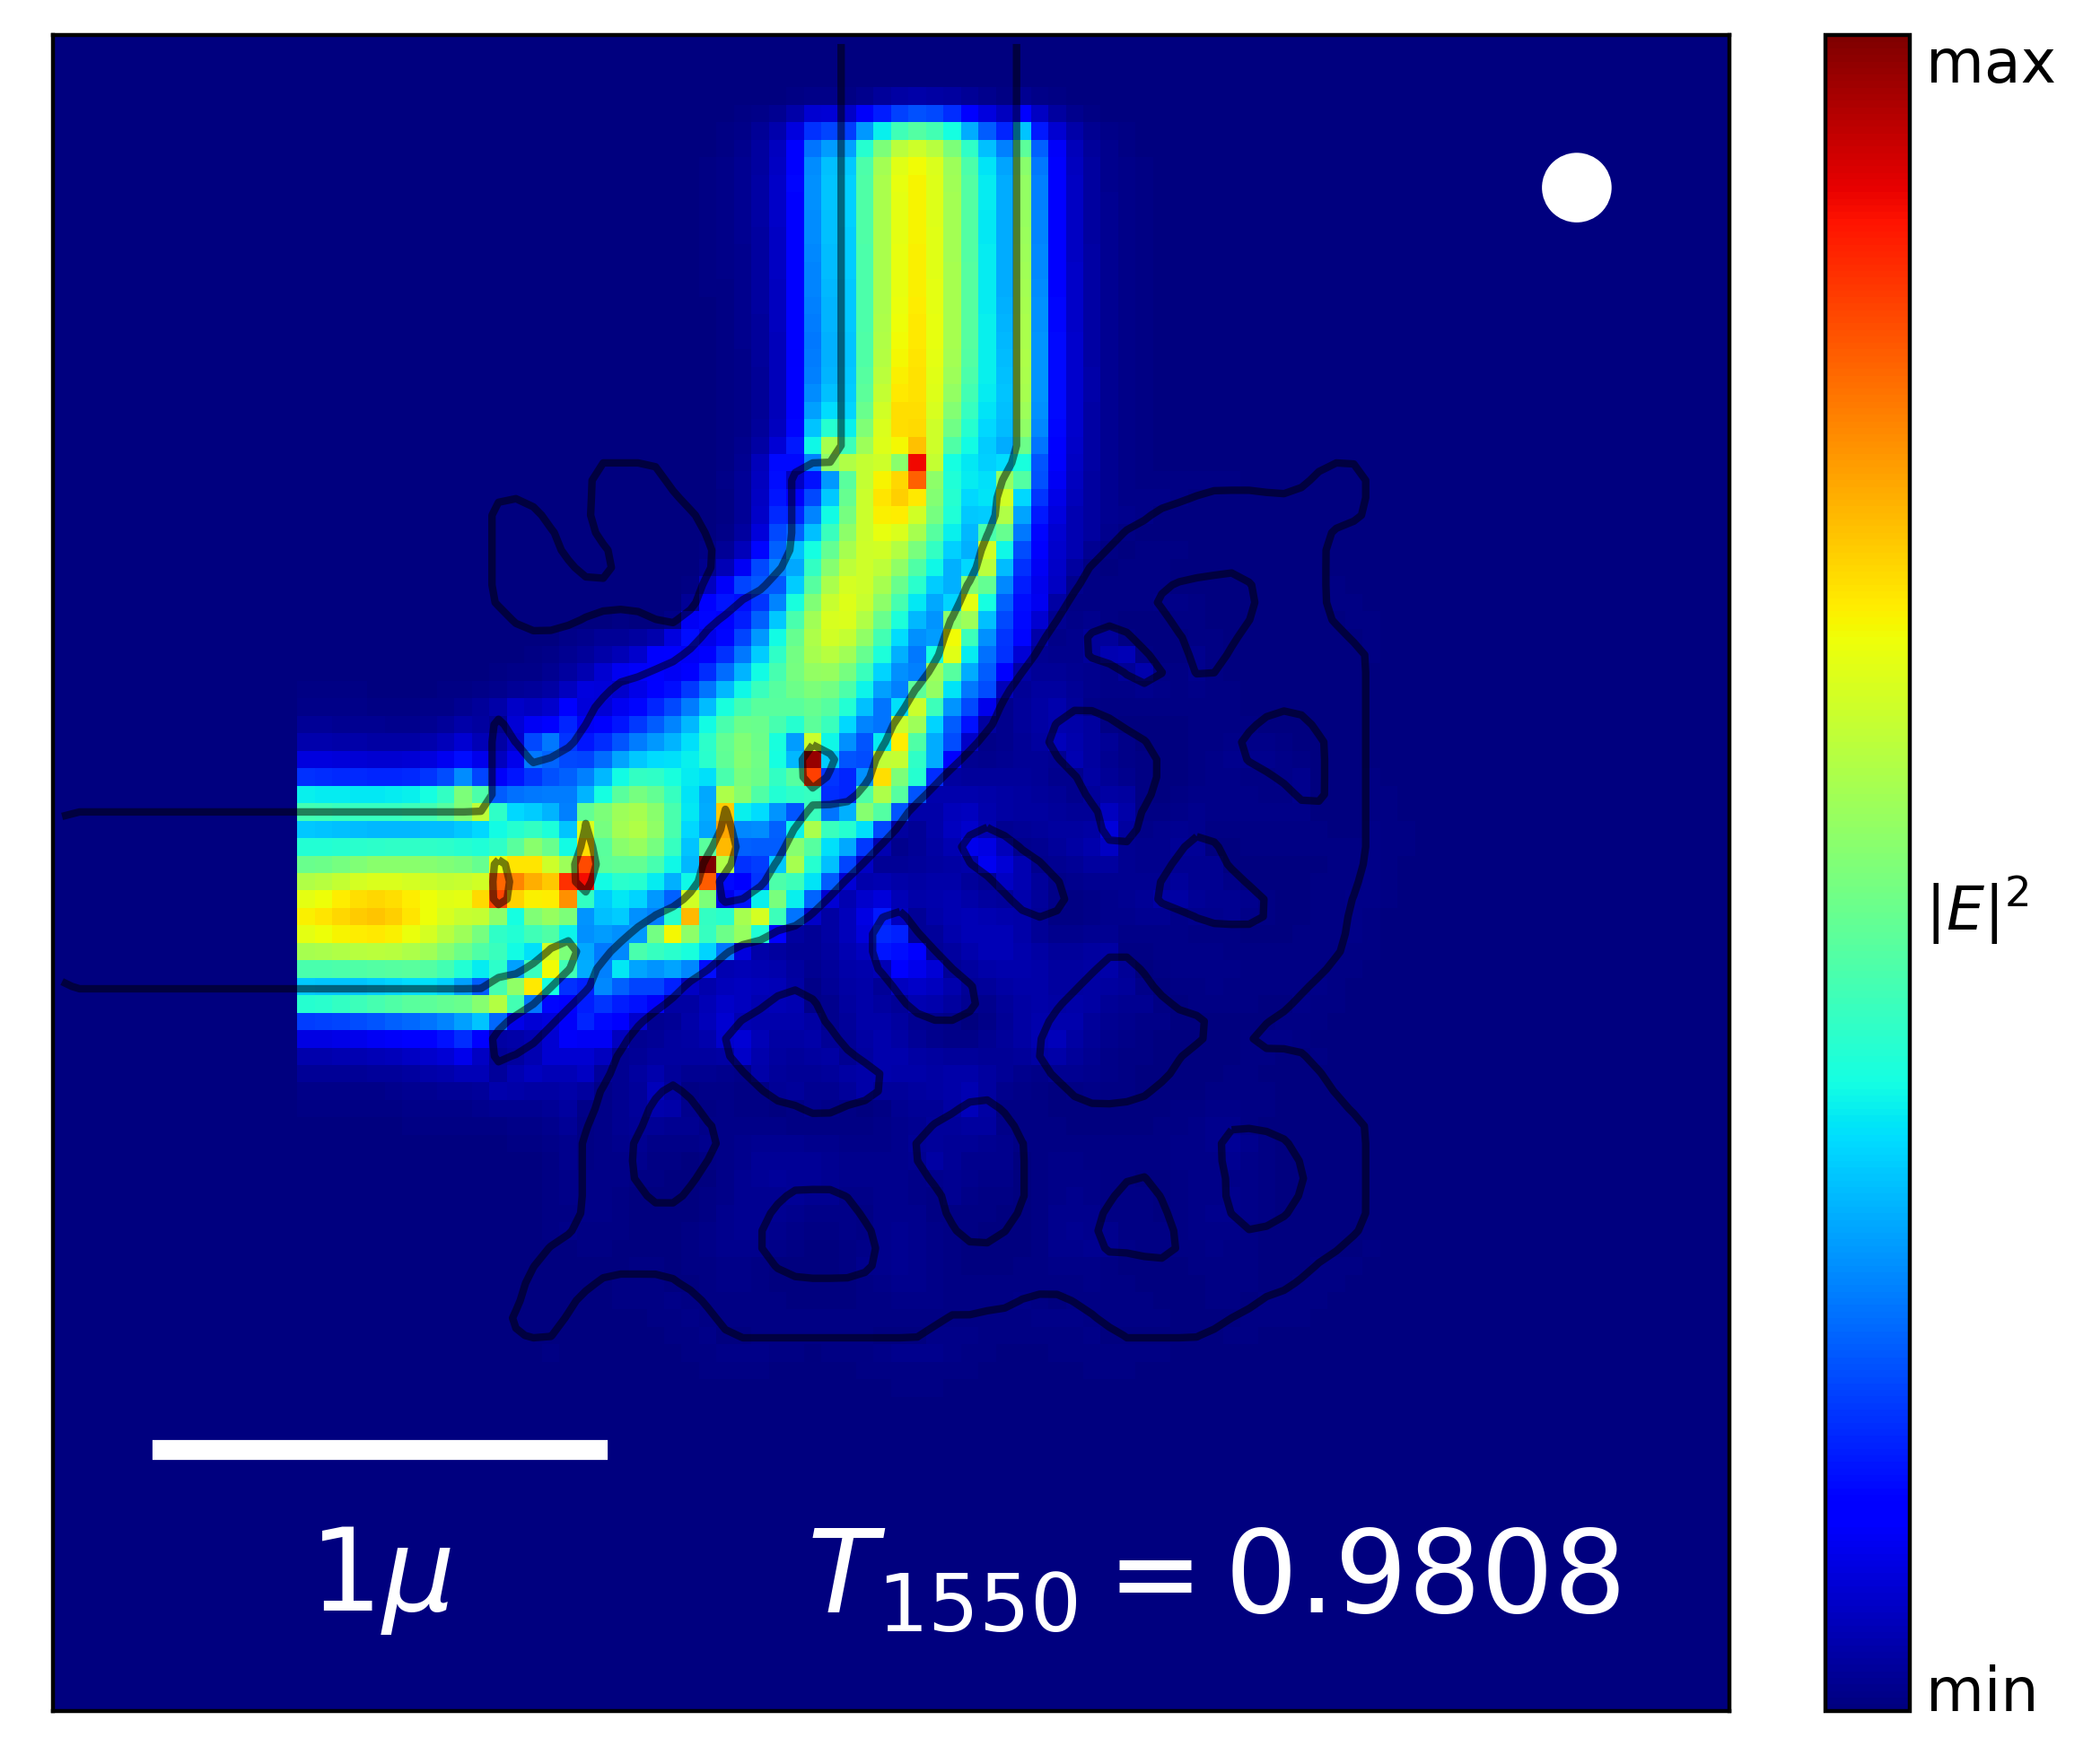
\includegraphics[width=0.33\textwidth]{image/results/bend/L-BFGS-B/visualize_field_fab_128.png} \\
    \hline
      \multirow{2}{*}{256} &
      
\includegraphics[width=0.20\textwidth]{image/results/bend/L-BFGS-B/visualize_eps_cont_256.png} &
      
\includegraphics[width=0.20\textwidth]{image/results/bend/L-BFGS-B/visualize_eps_disc_256.png} &
      
\includegraphics[width=0.20\textwidth]{image/results/bend/L-BFGS-B/visualize_eps_fab_256.png} \\
      \cline{2-4}
      &
      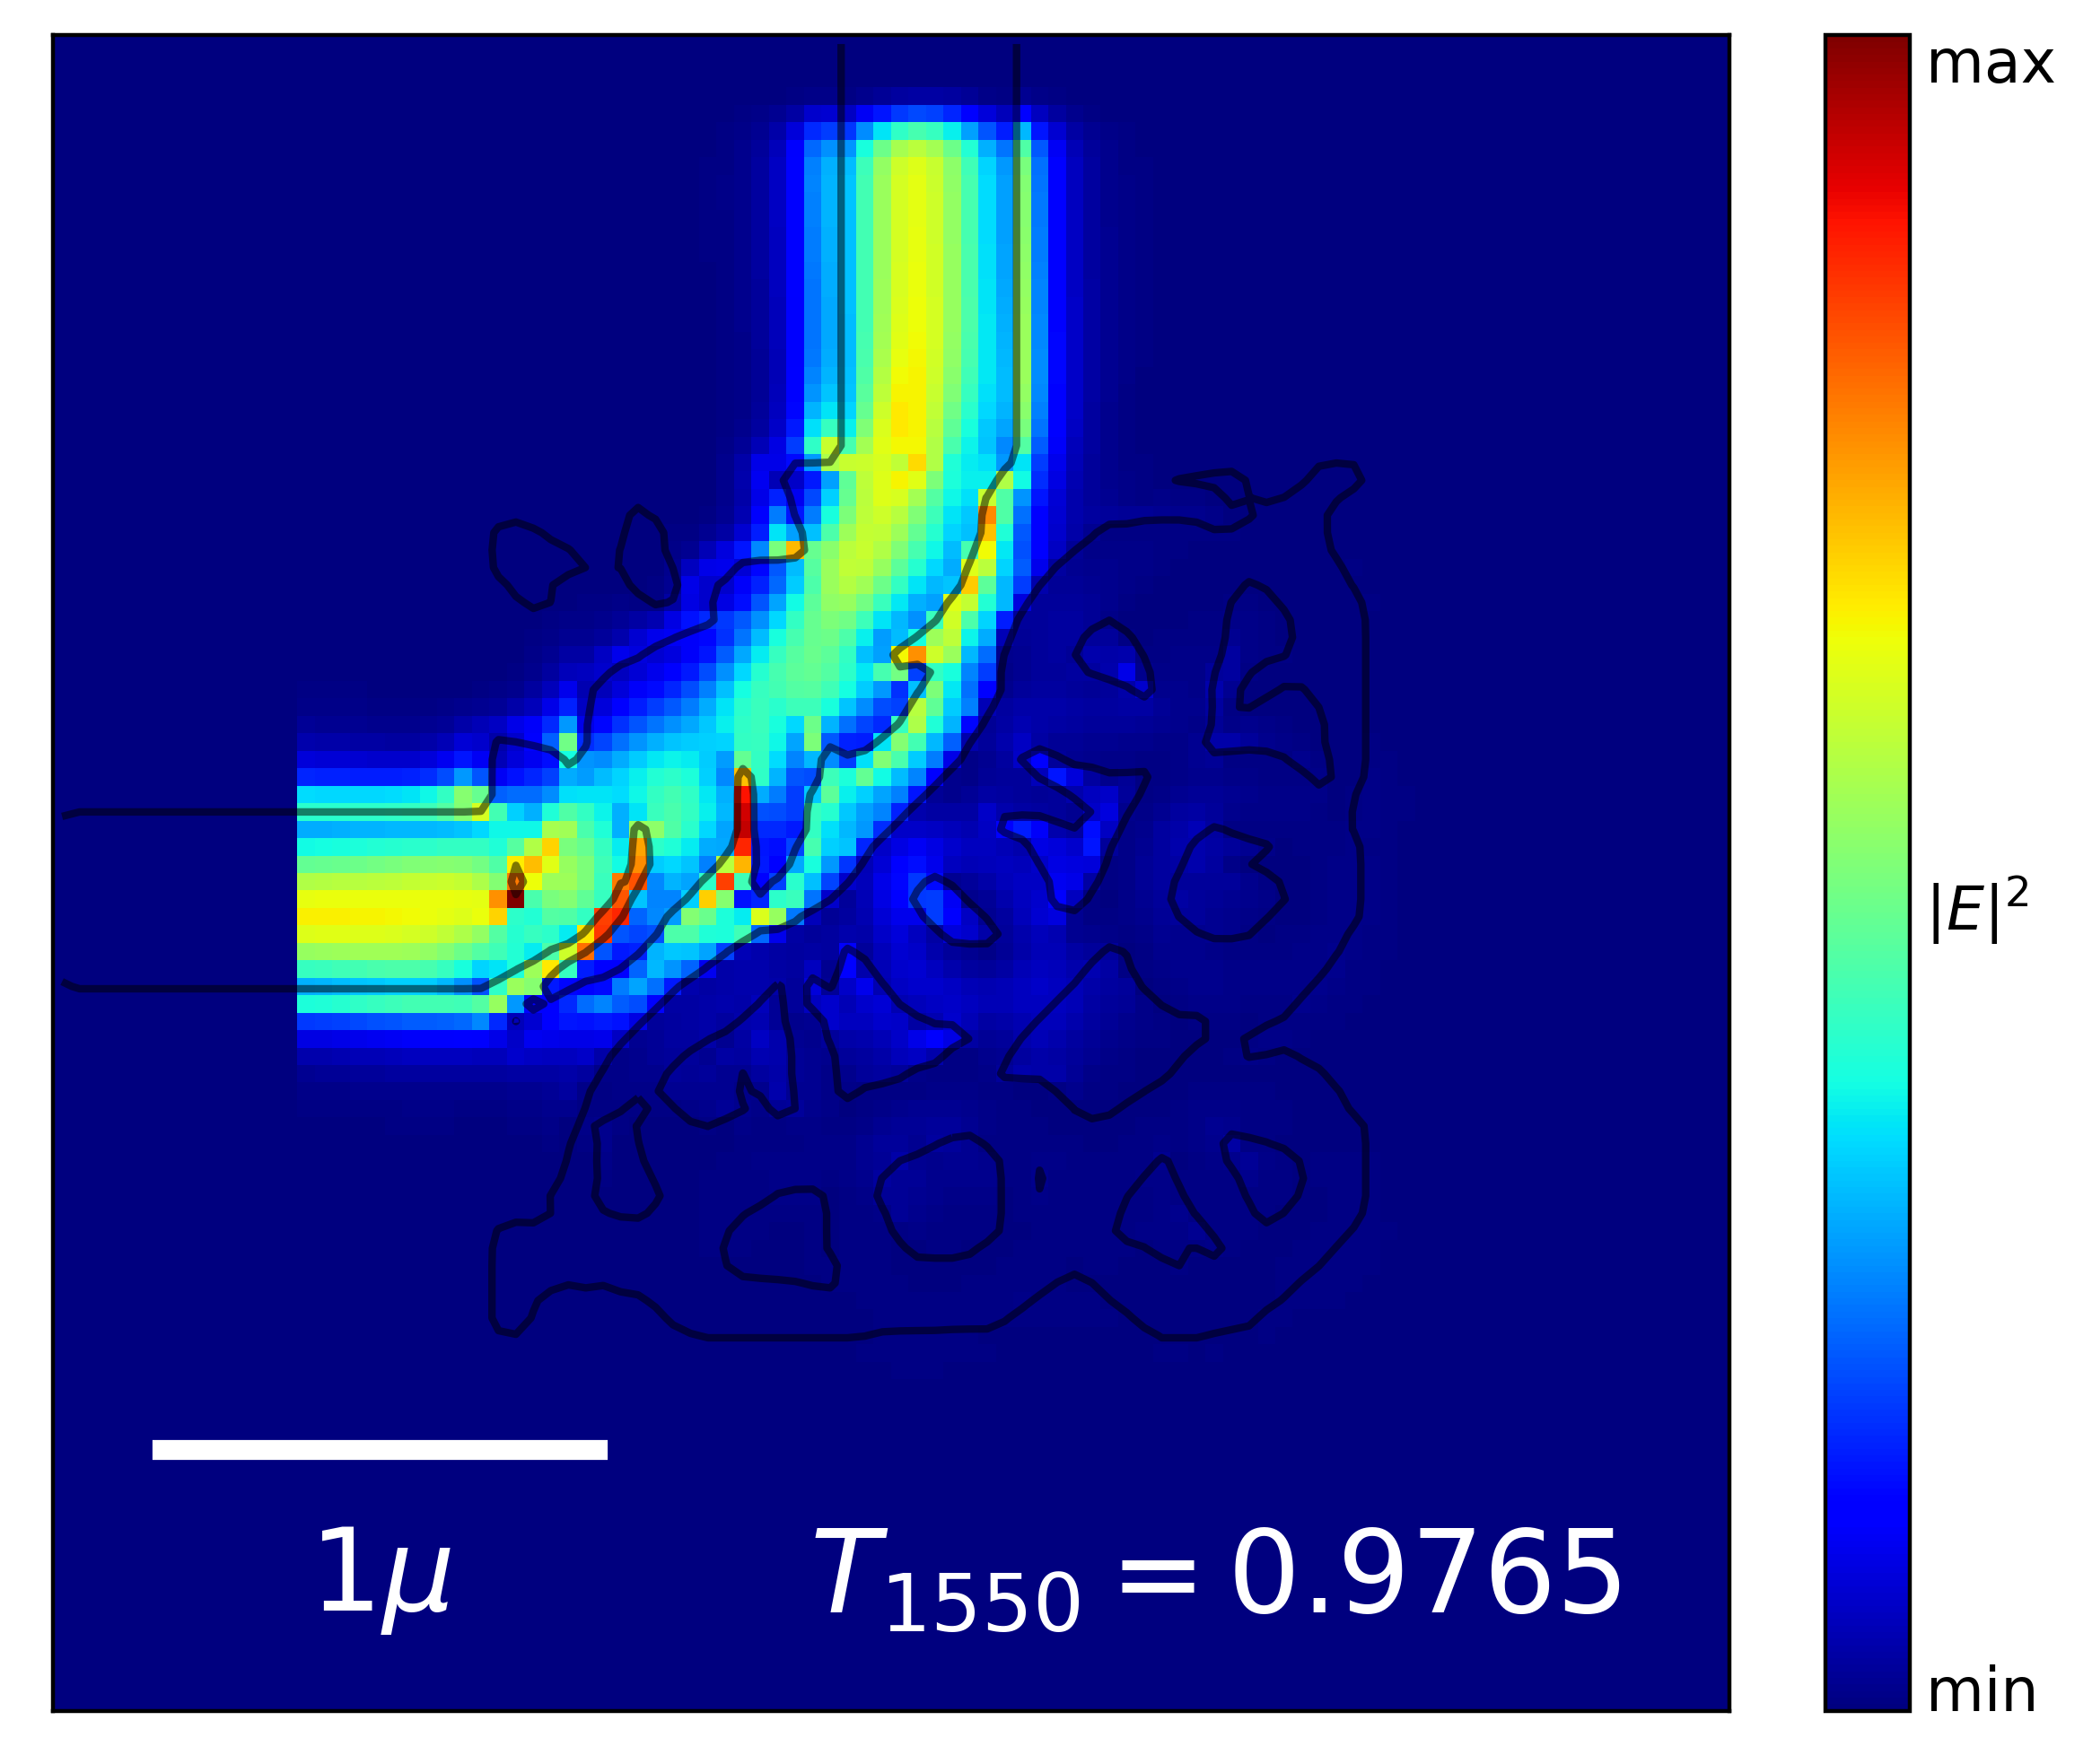
\includegraphics[width=0.33\textwidth]{image/results/bend/L-BFGS-B/visualize_field_cont_256.png} &
      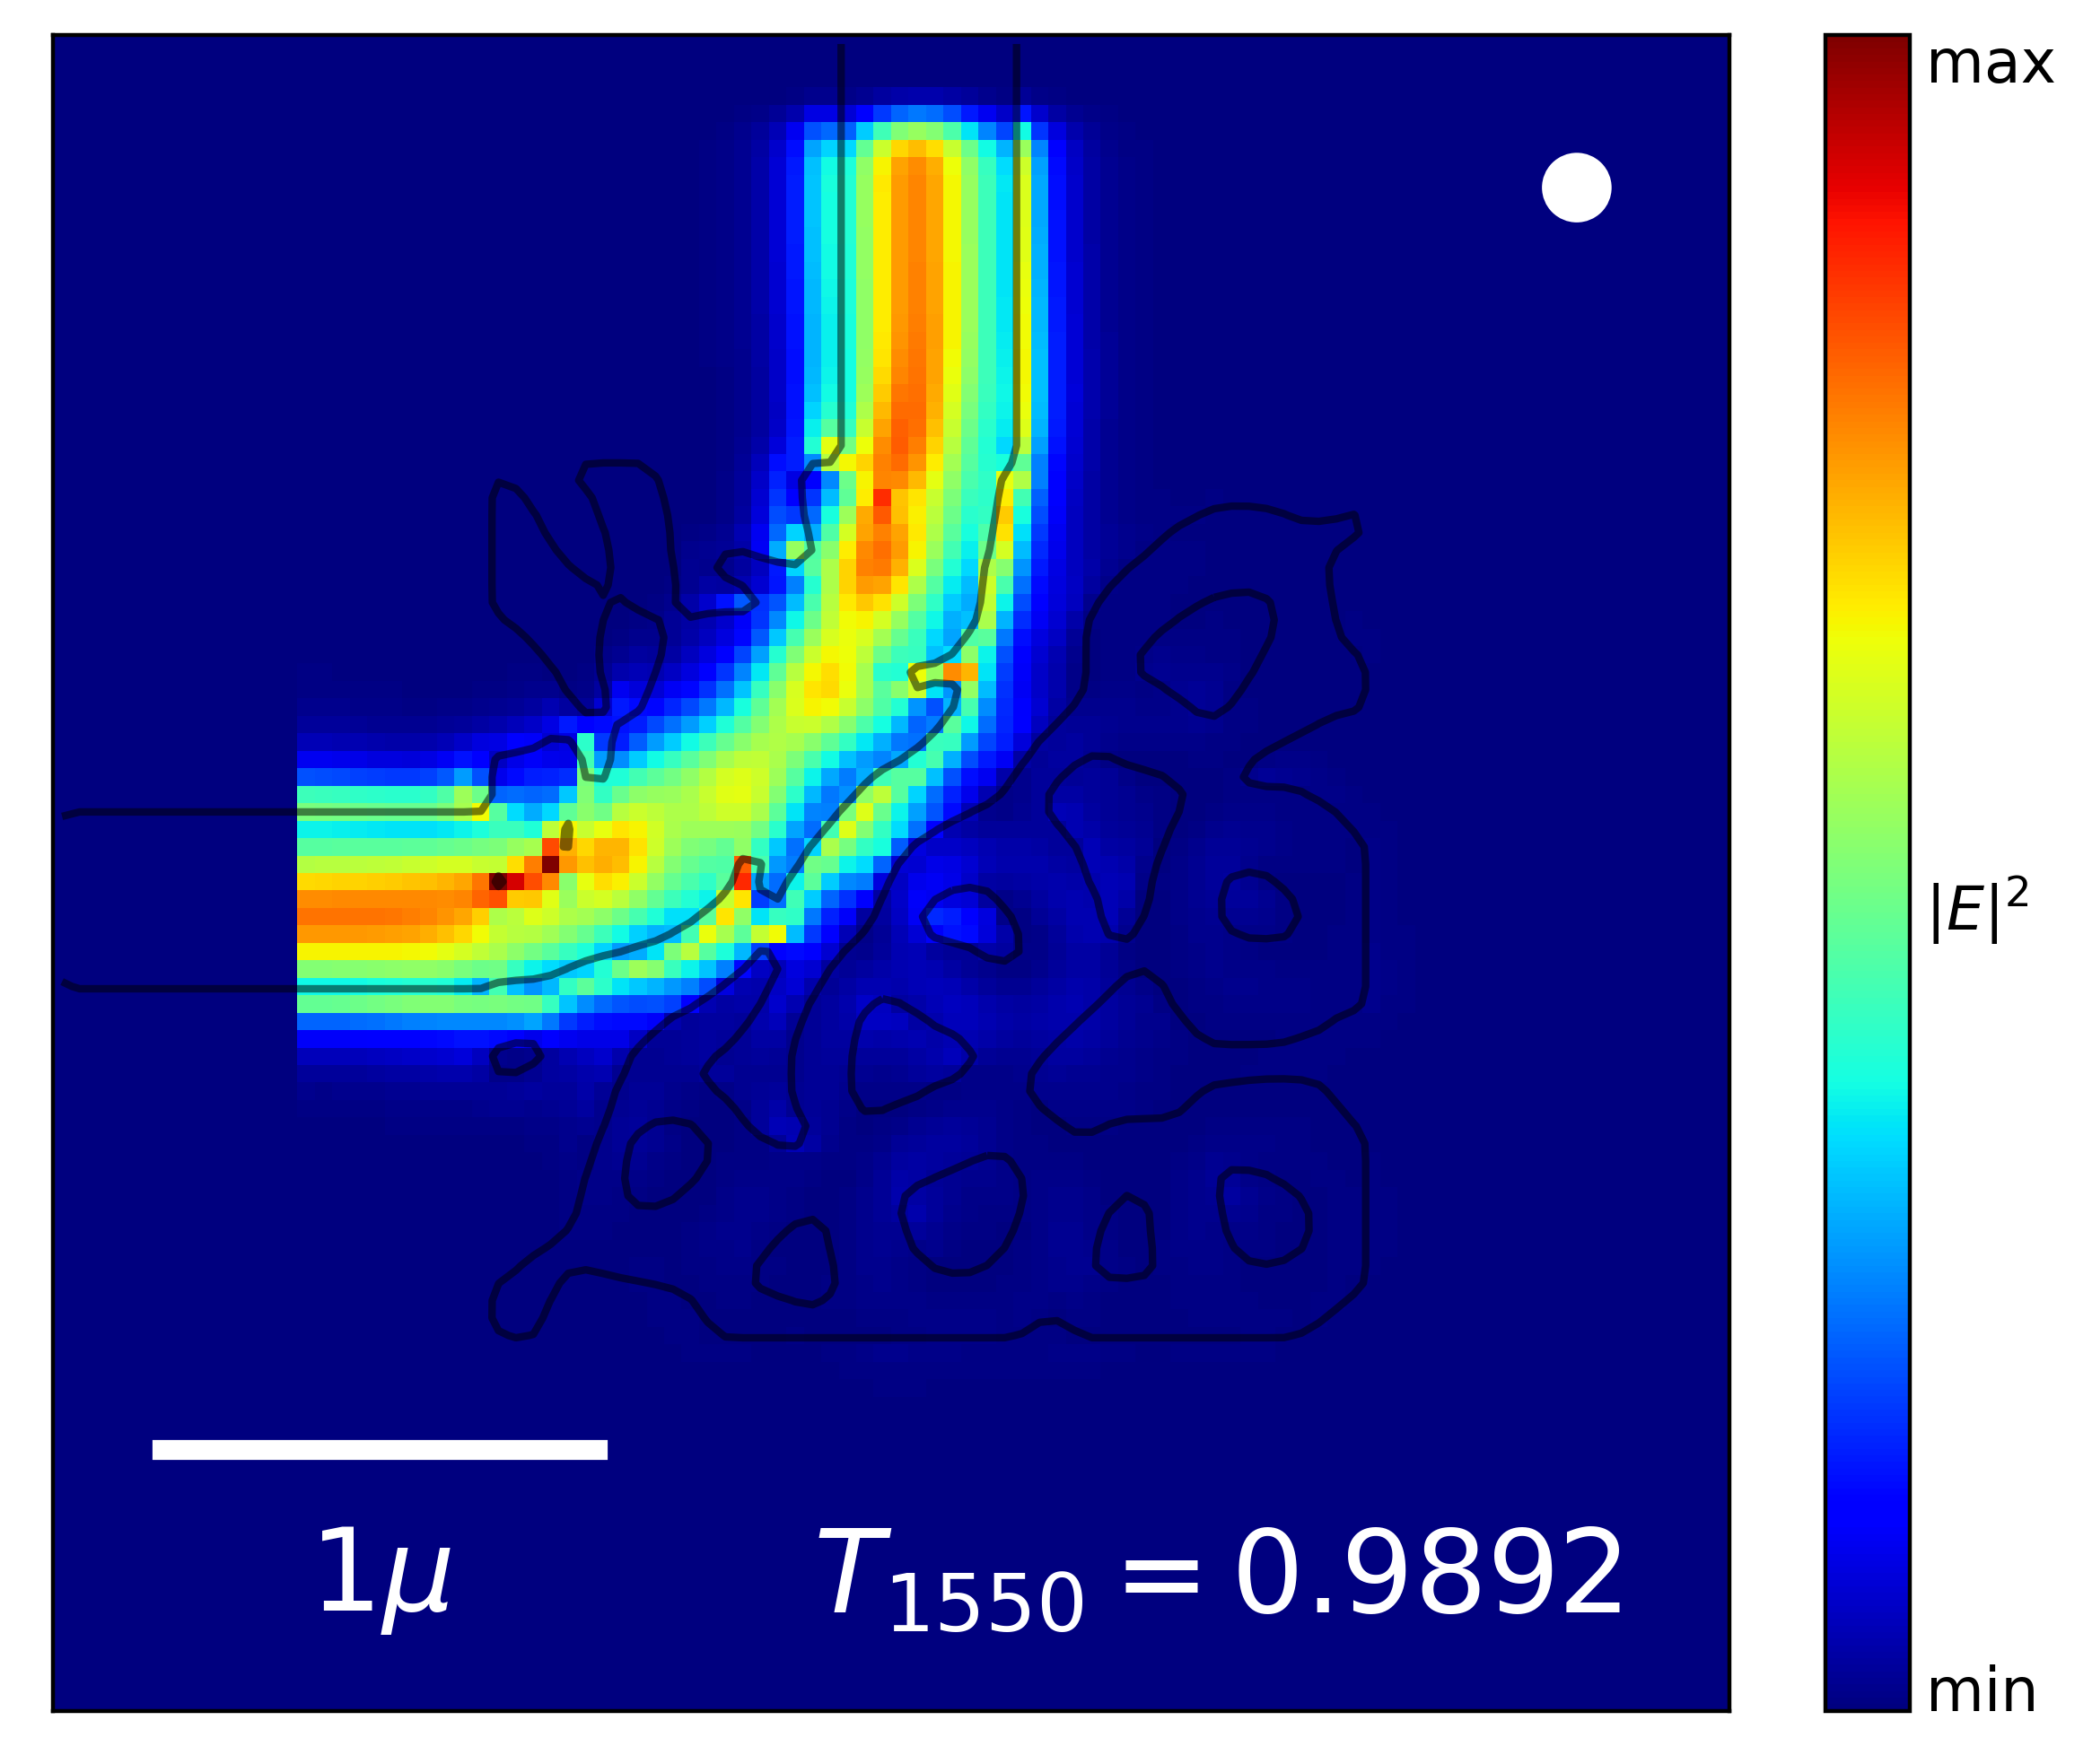
\includegraphics[width=0.33\textwidth]{image/results/bend/L-BFGS-B/visualize_field_disc_256.png} &
      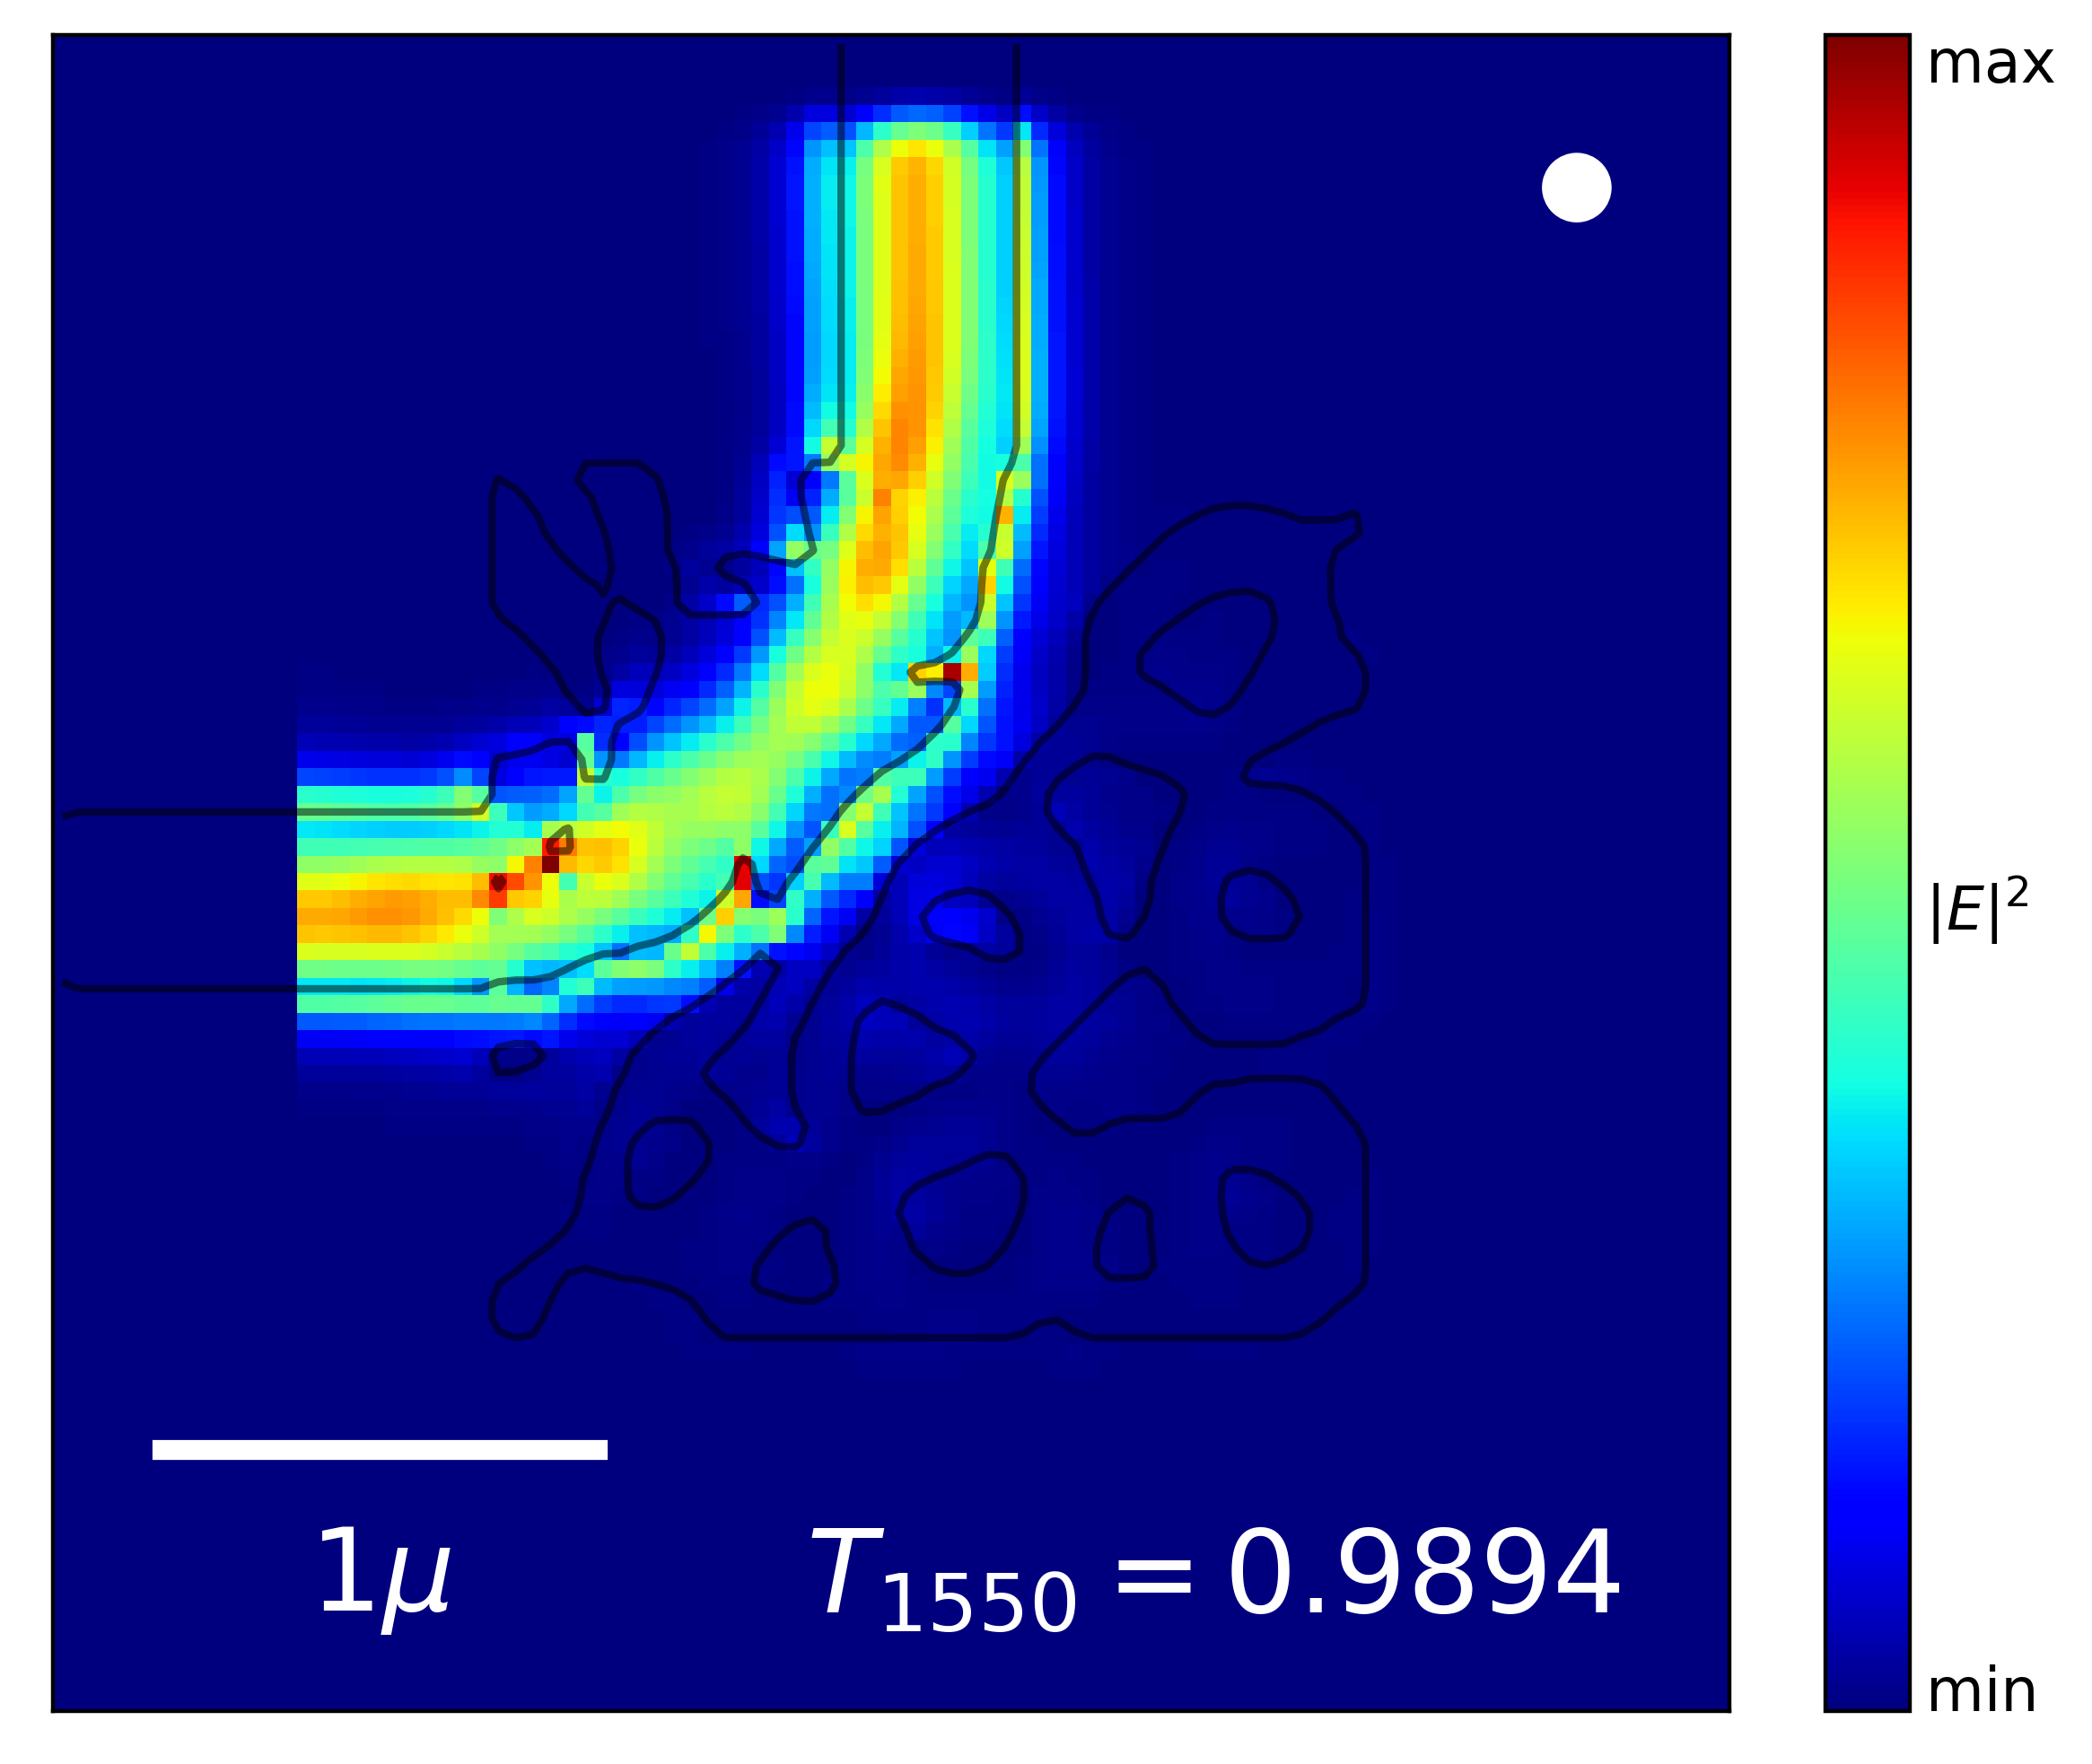
\includegraphics[width=0.33\textwidth]{image/results/bend/L-BFGS-B/visualize_field_fab_256.png} \\
    \hline
      \multirow{2}{*}{512} &
      
\includegraphics[width=0.20\textwidth]{image/results/bend/L-BFGS-B/visualize_eps_cont_512.png} &
      
\includegraphics[width=0.20\textwidth]{image/results/bend/L-BFGS-B/visualize_eps_disc_512.png} &
      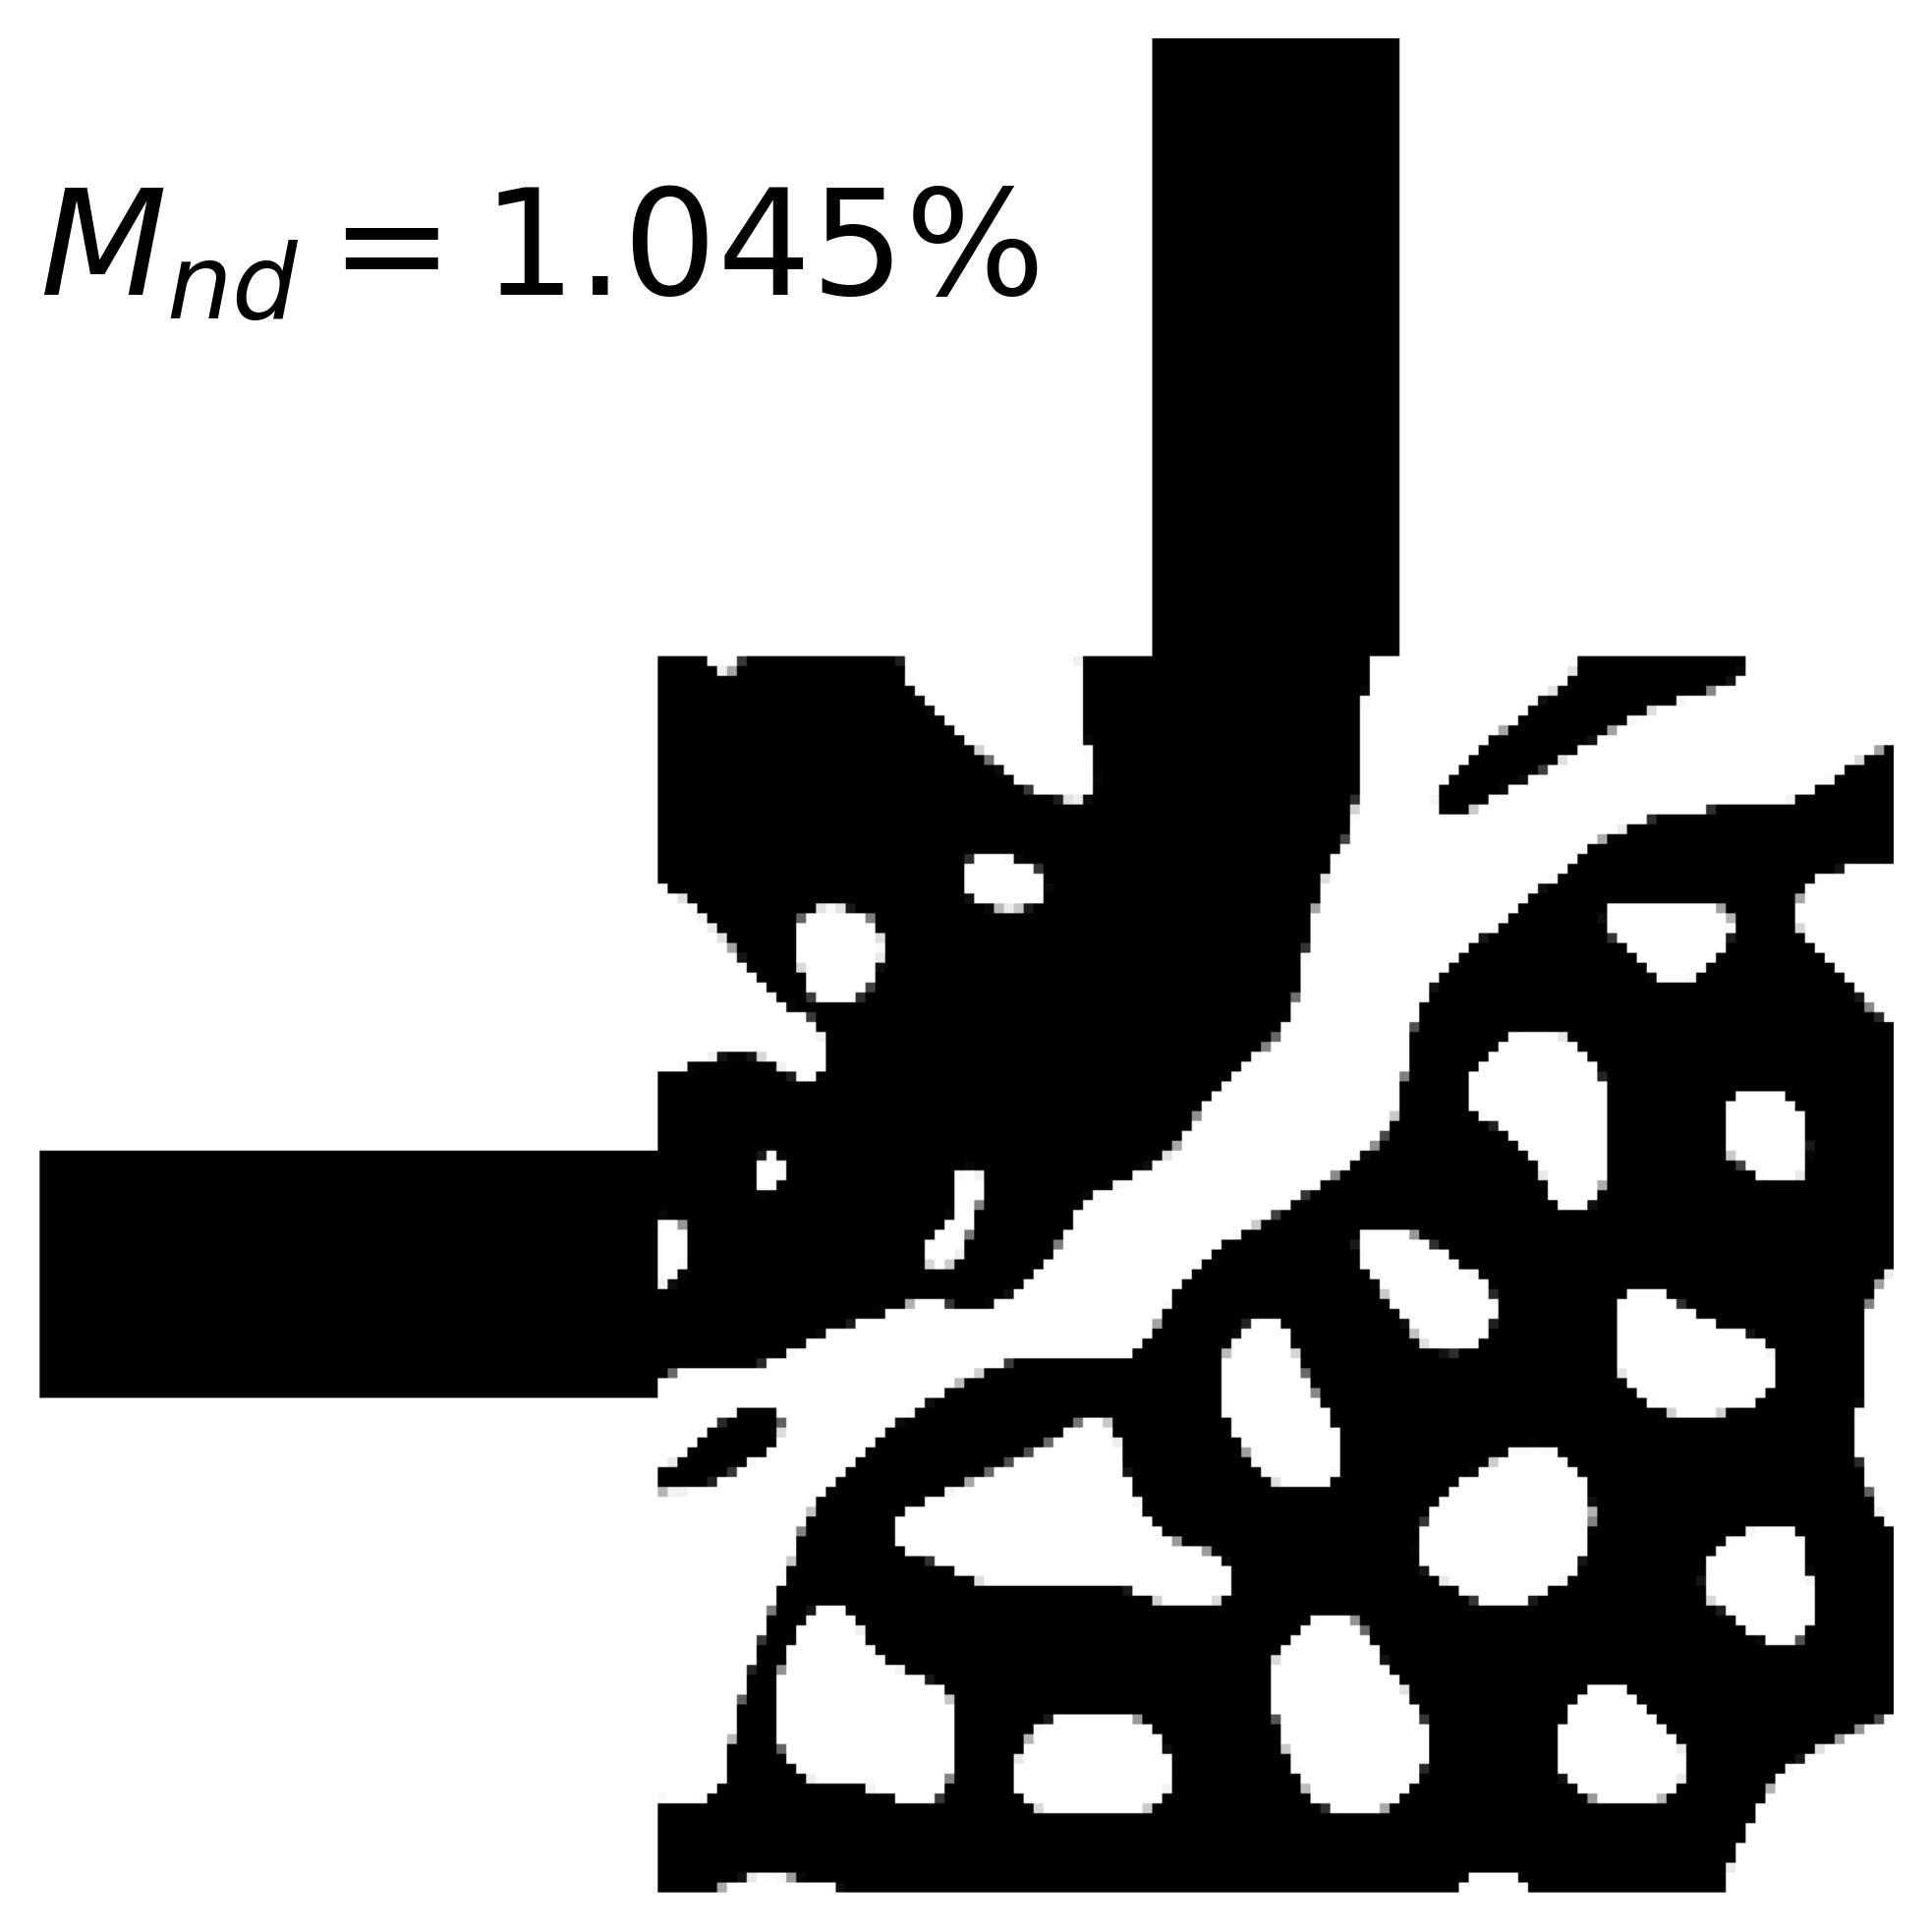
\includegraphics[width=0.20\textwidth]{image/results/bend/L-BFGS-B/visualize_eps_fab_512.png} \\
      \cline{2-4}
      &
      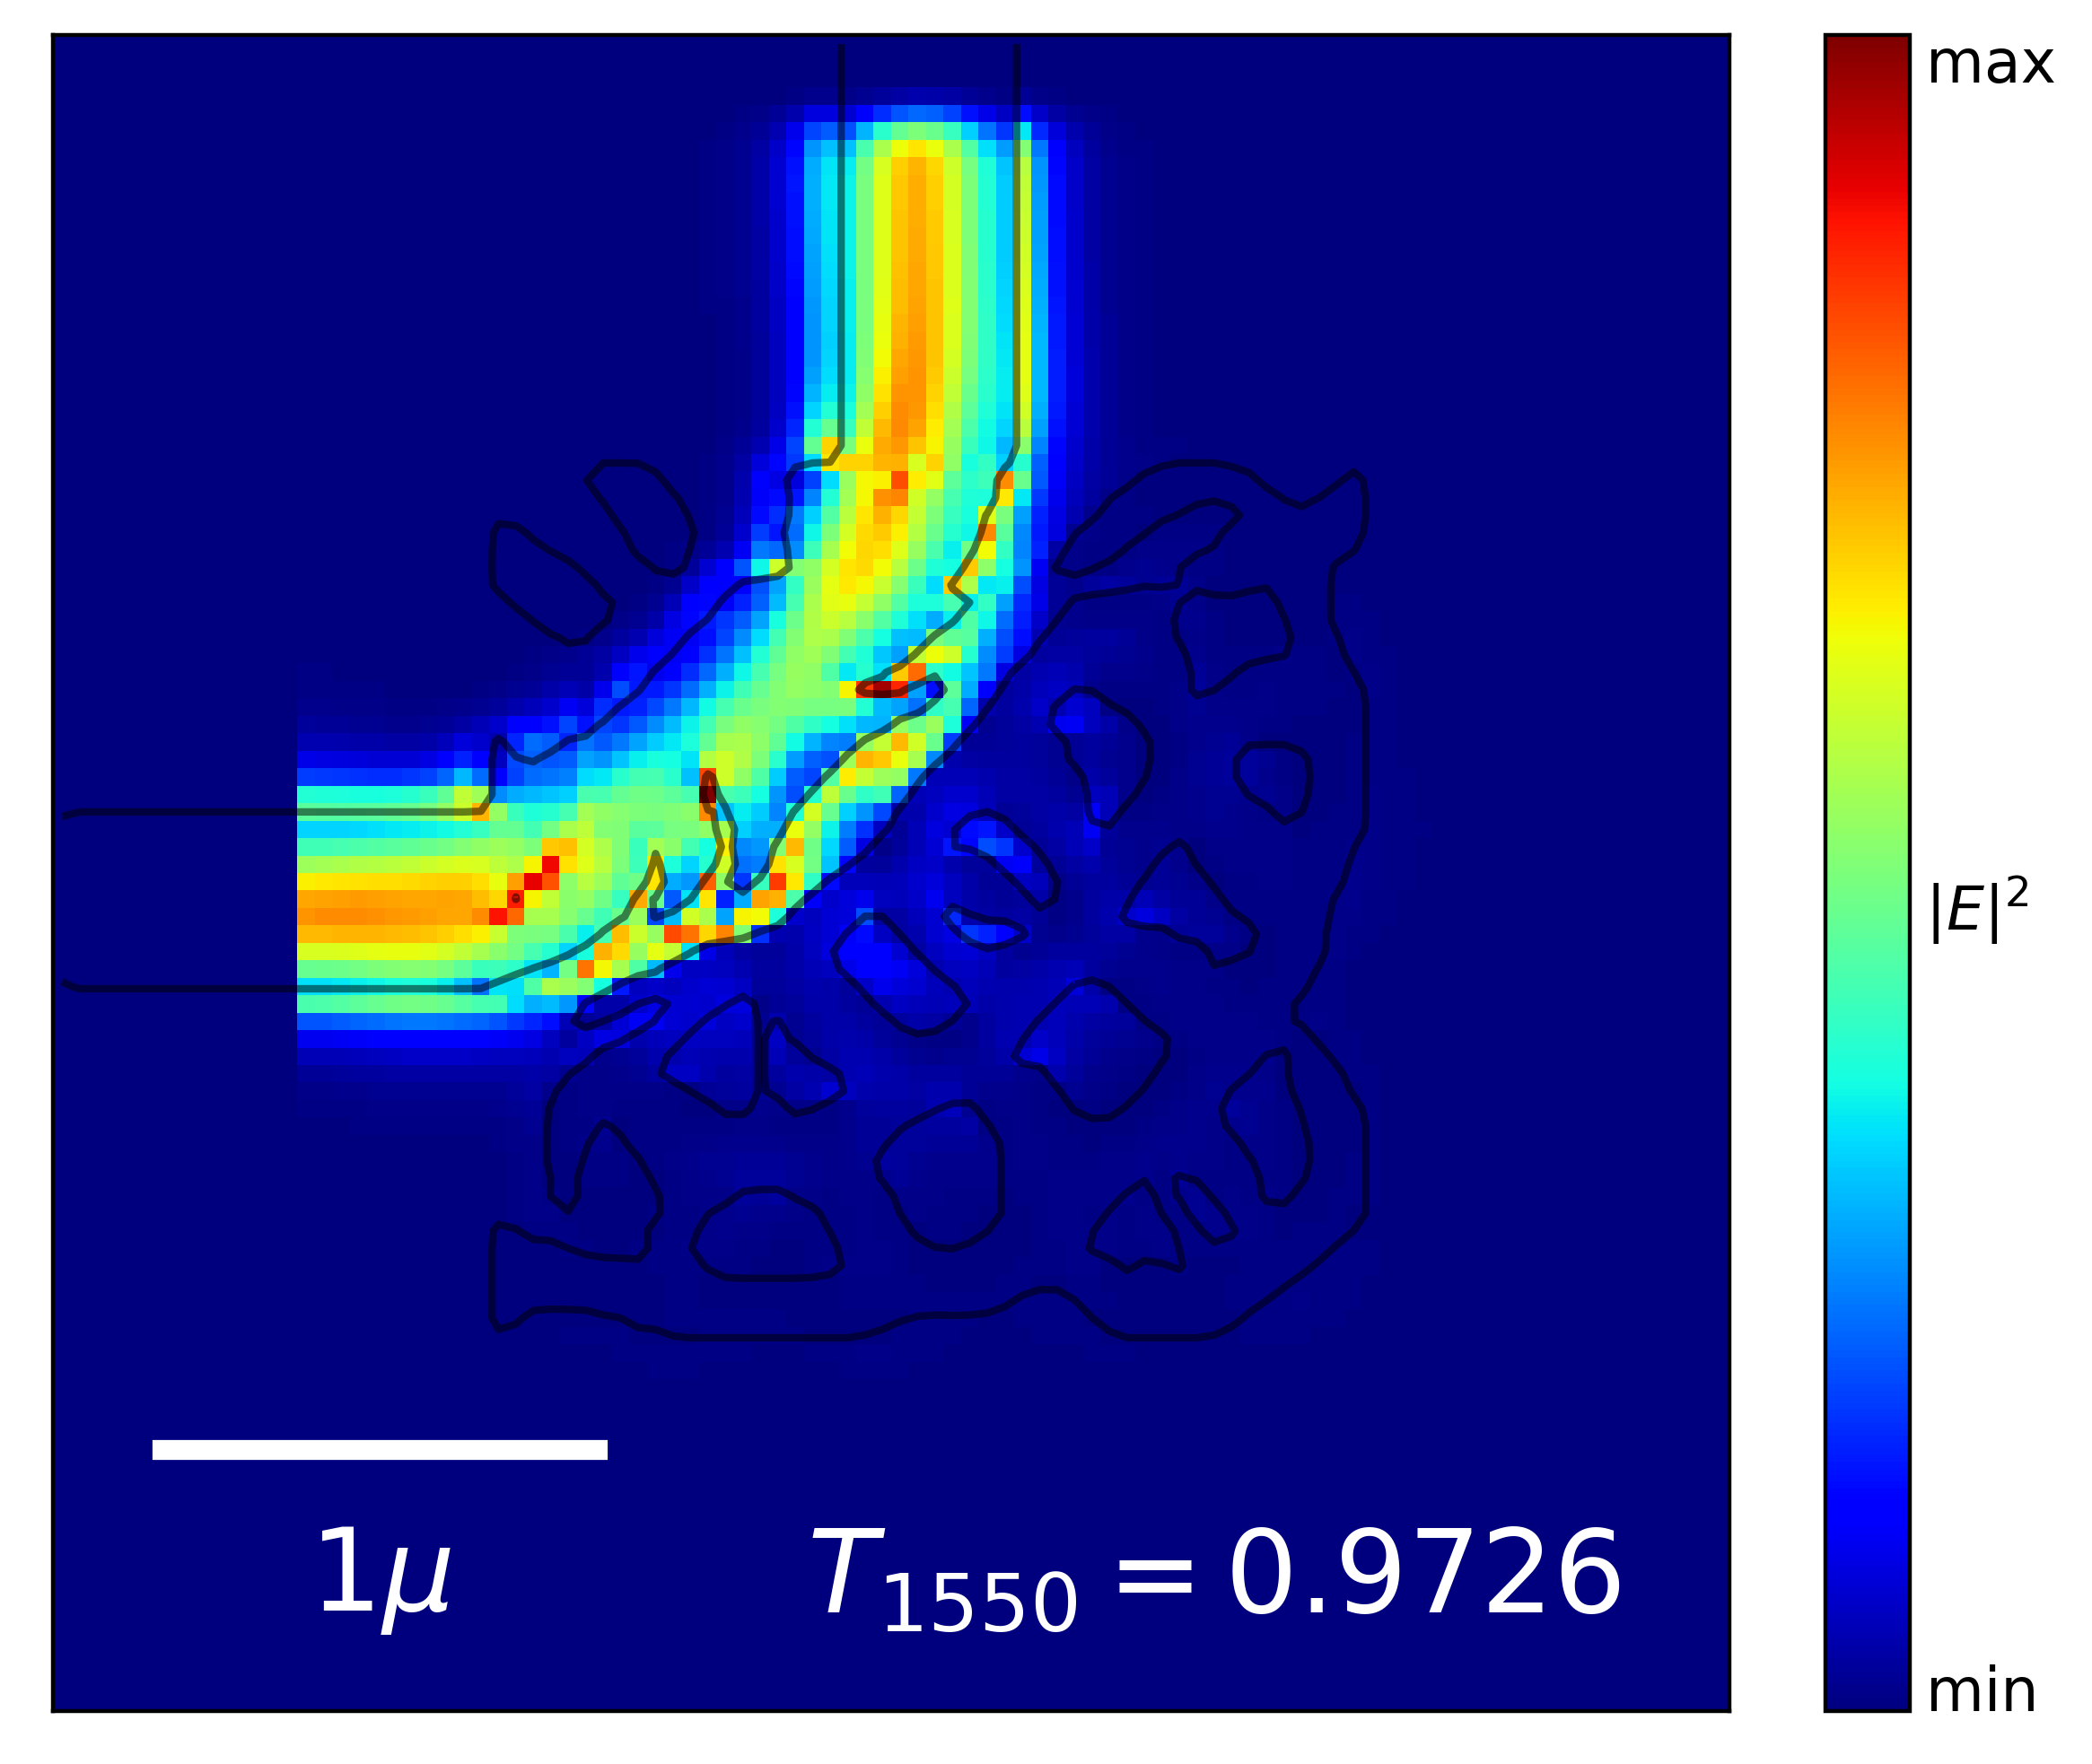
\includegraphics[width=0.33\textwidth]{image/results/bend/L-BFGS-B/visualize_field_cont_512.png} &
      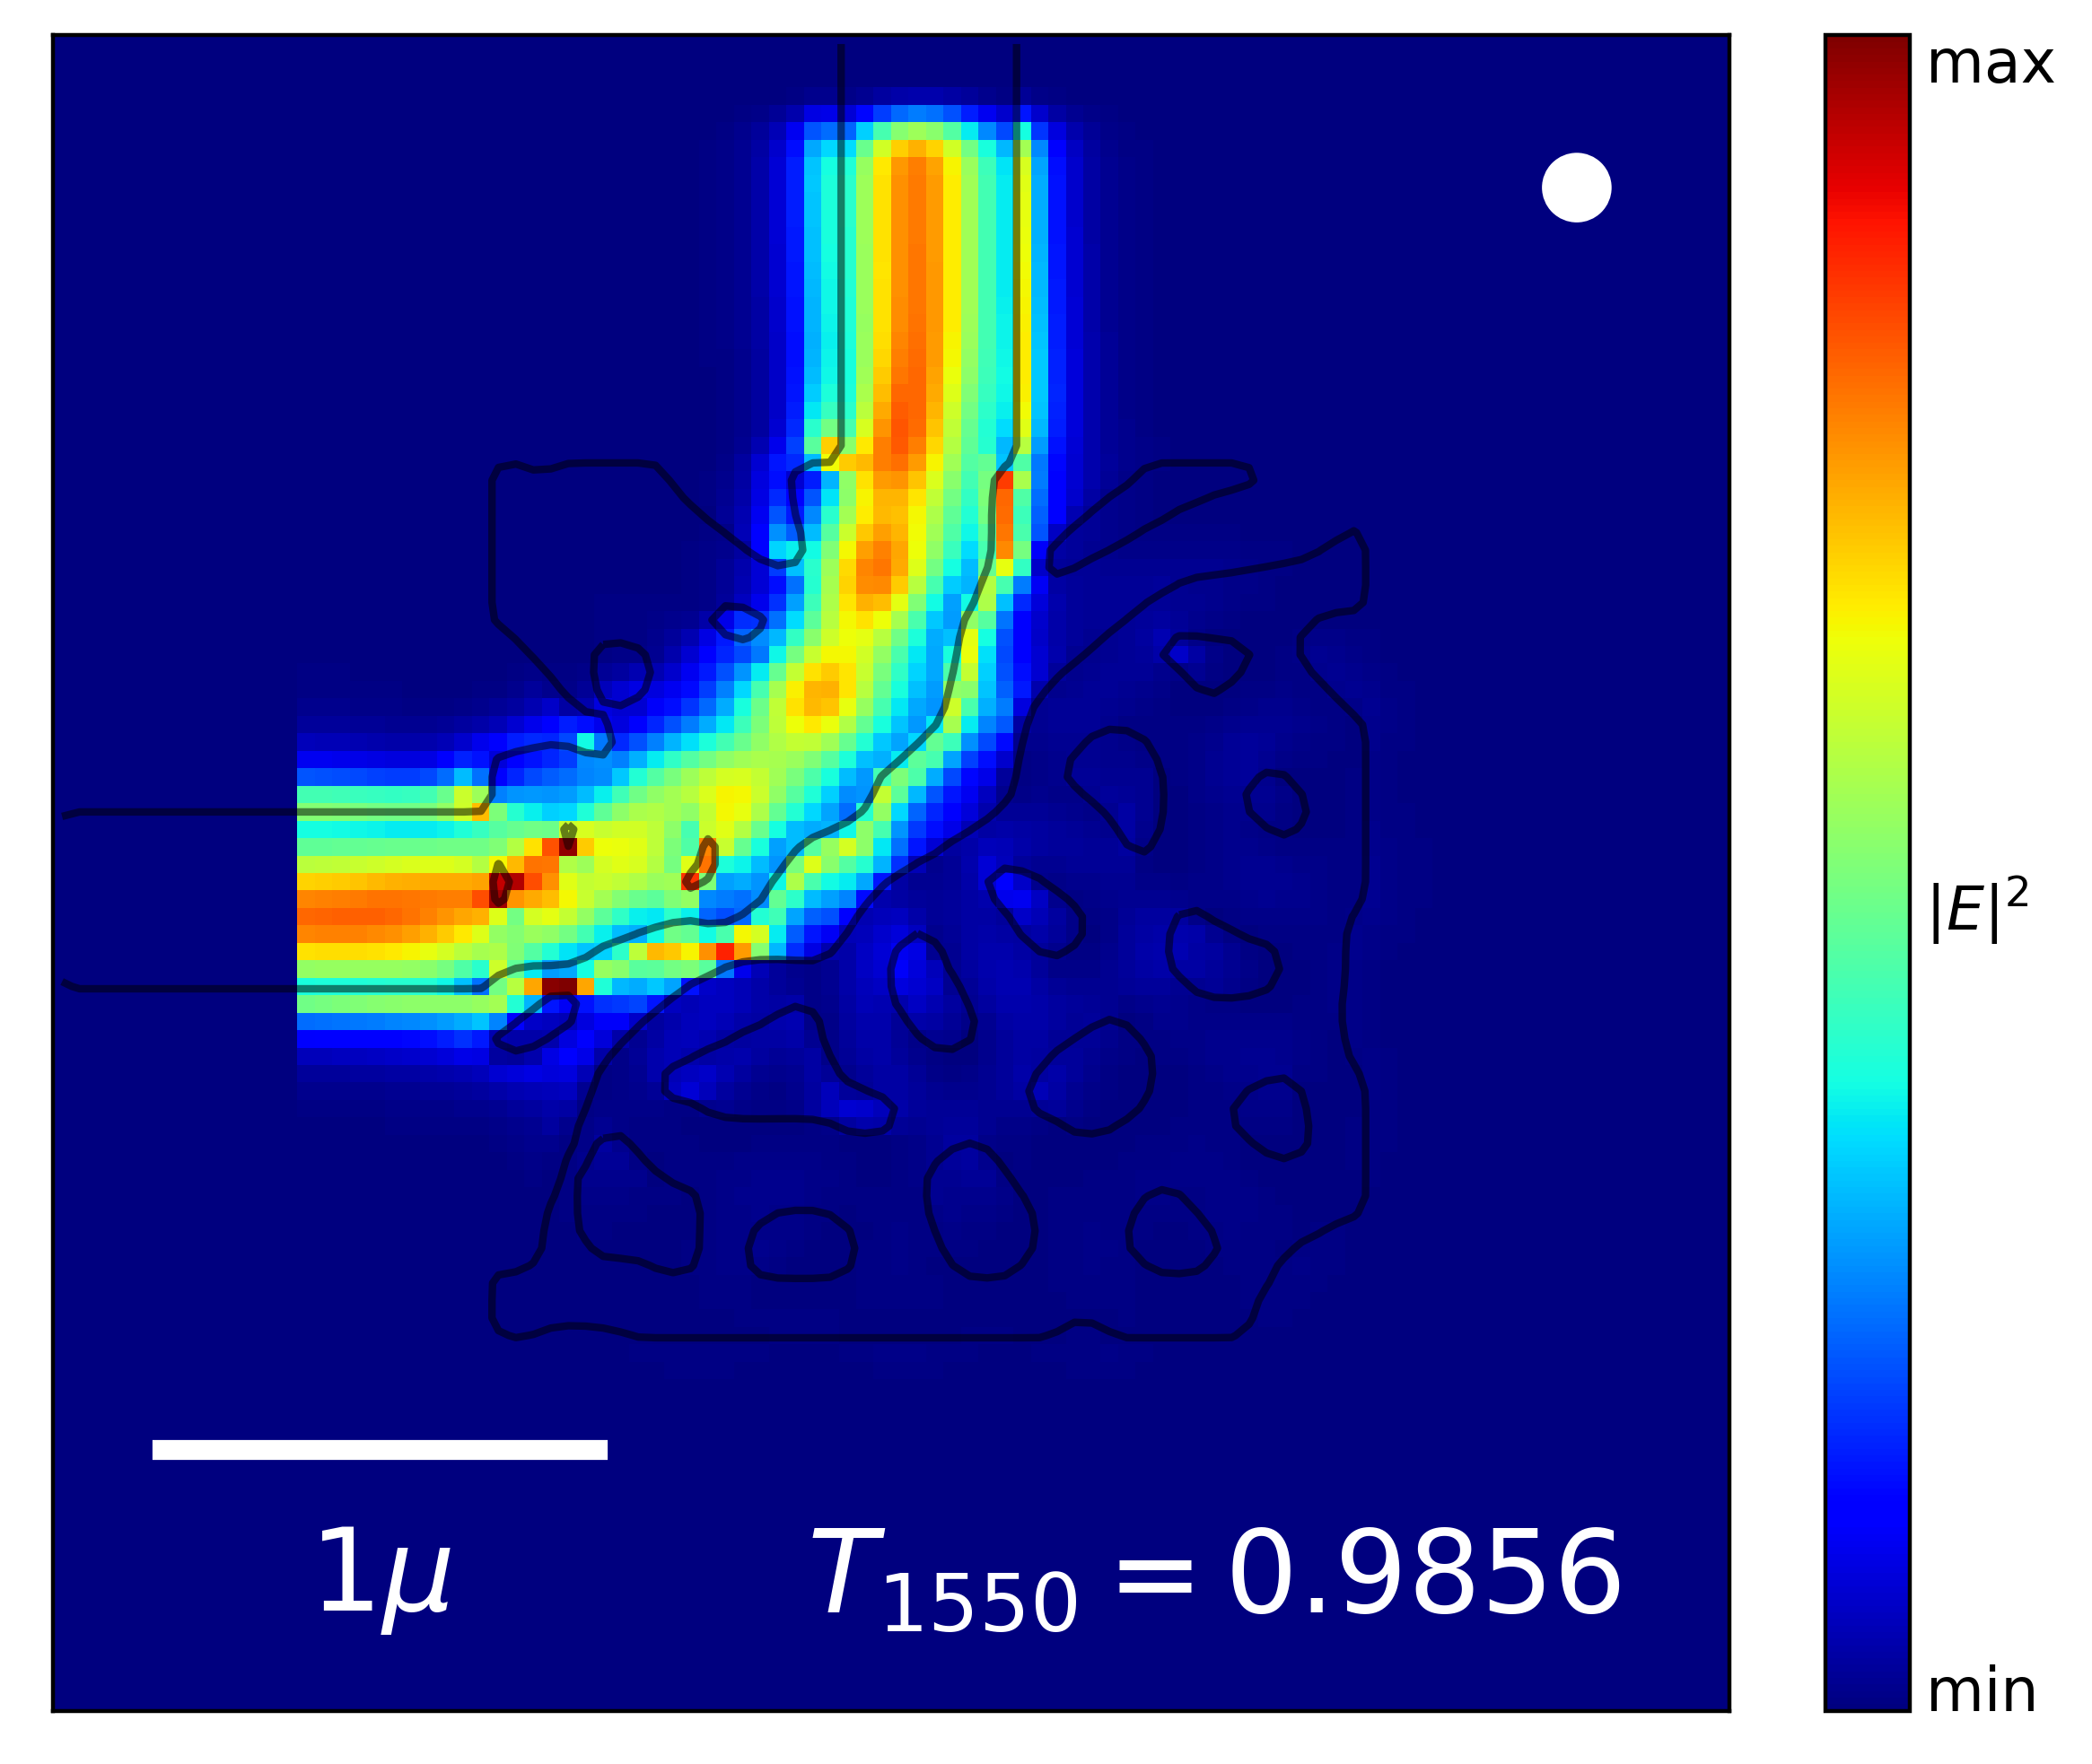
\includegraphics[width=0.33\textwidth]{image/results/bend/L-BFGS-B/visualize_field_disc_512.png} &
      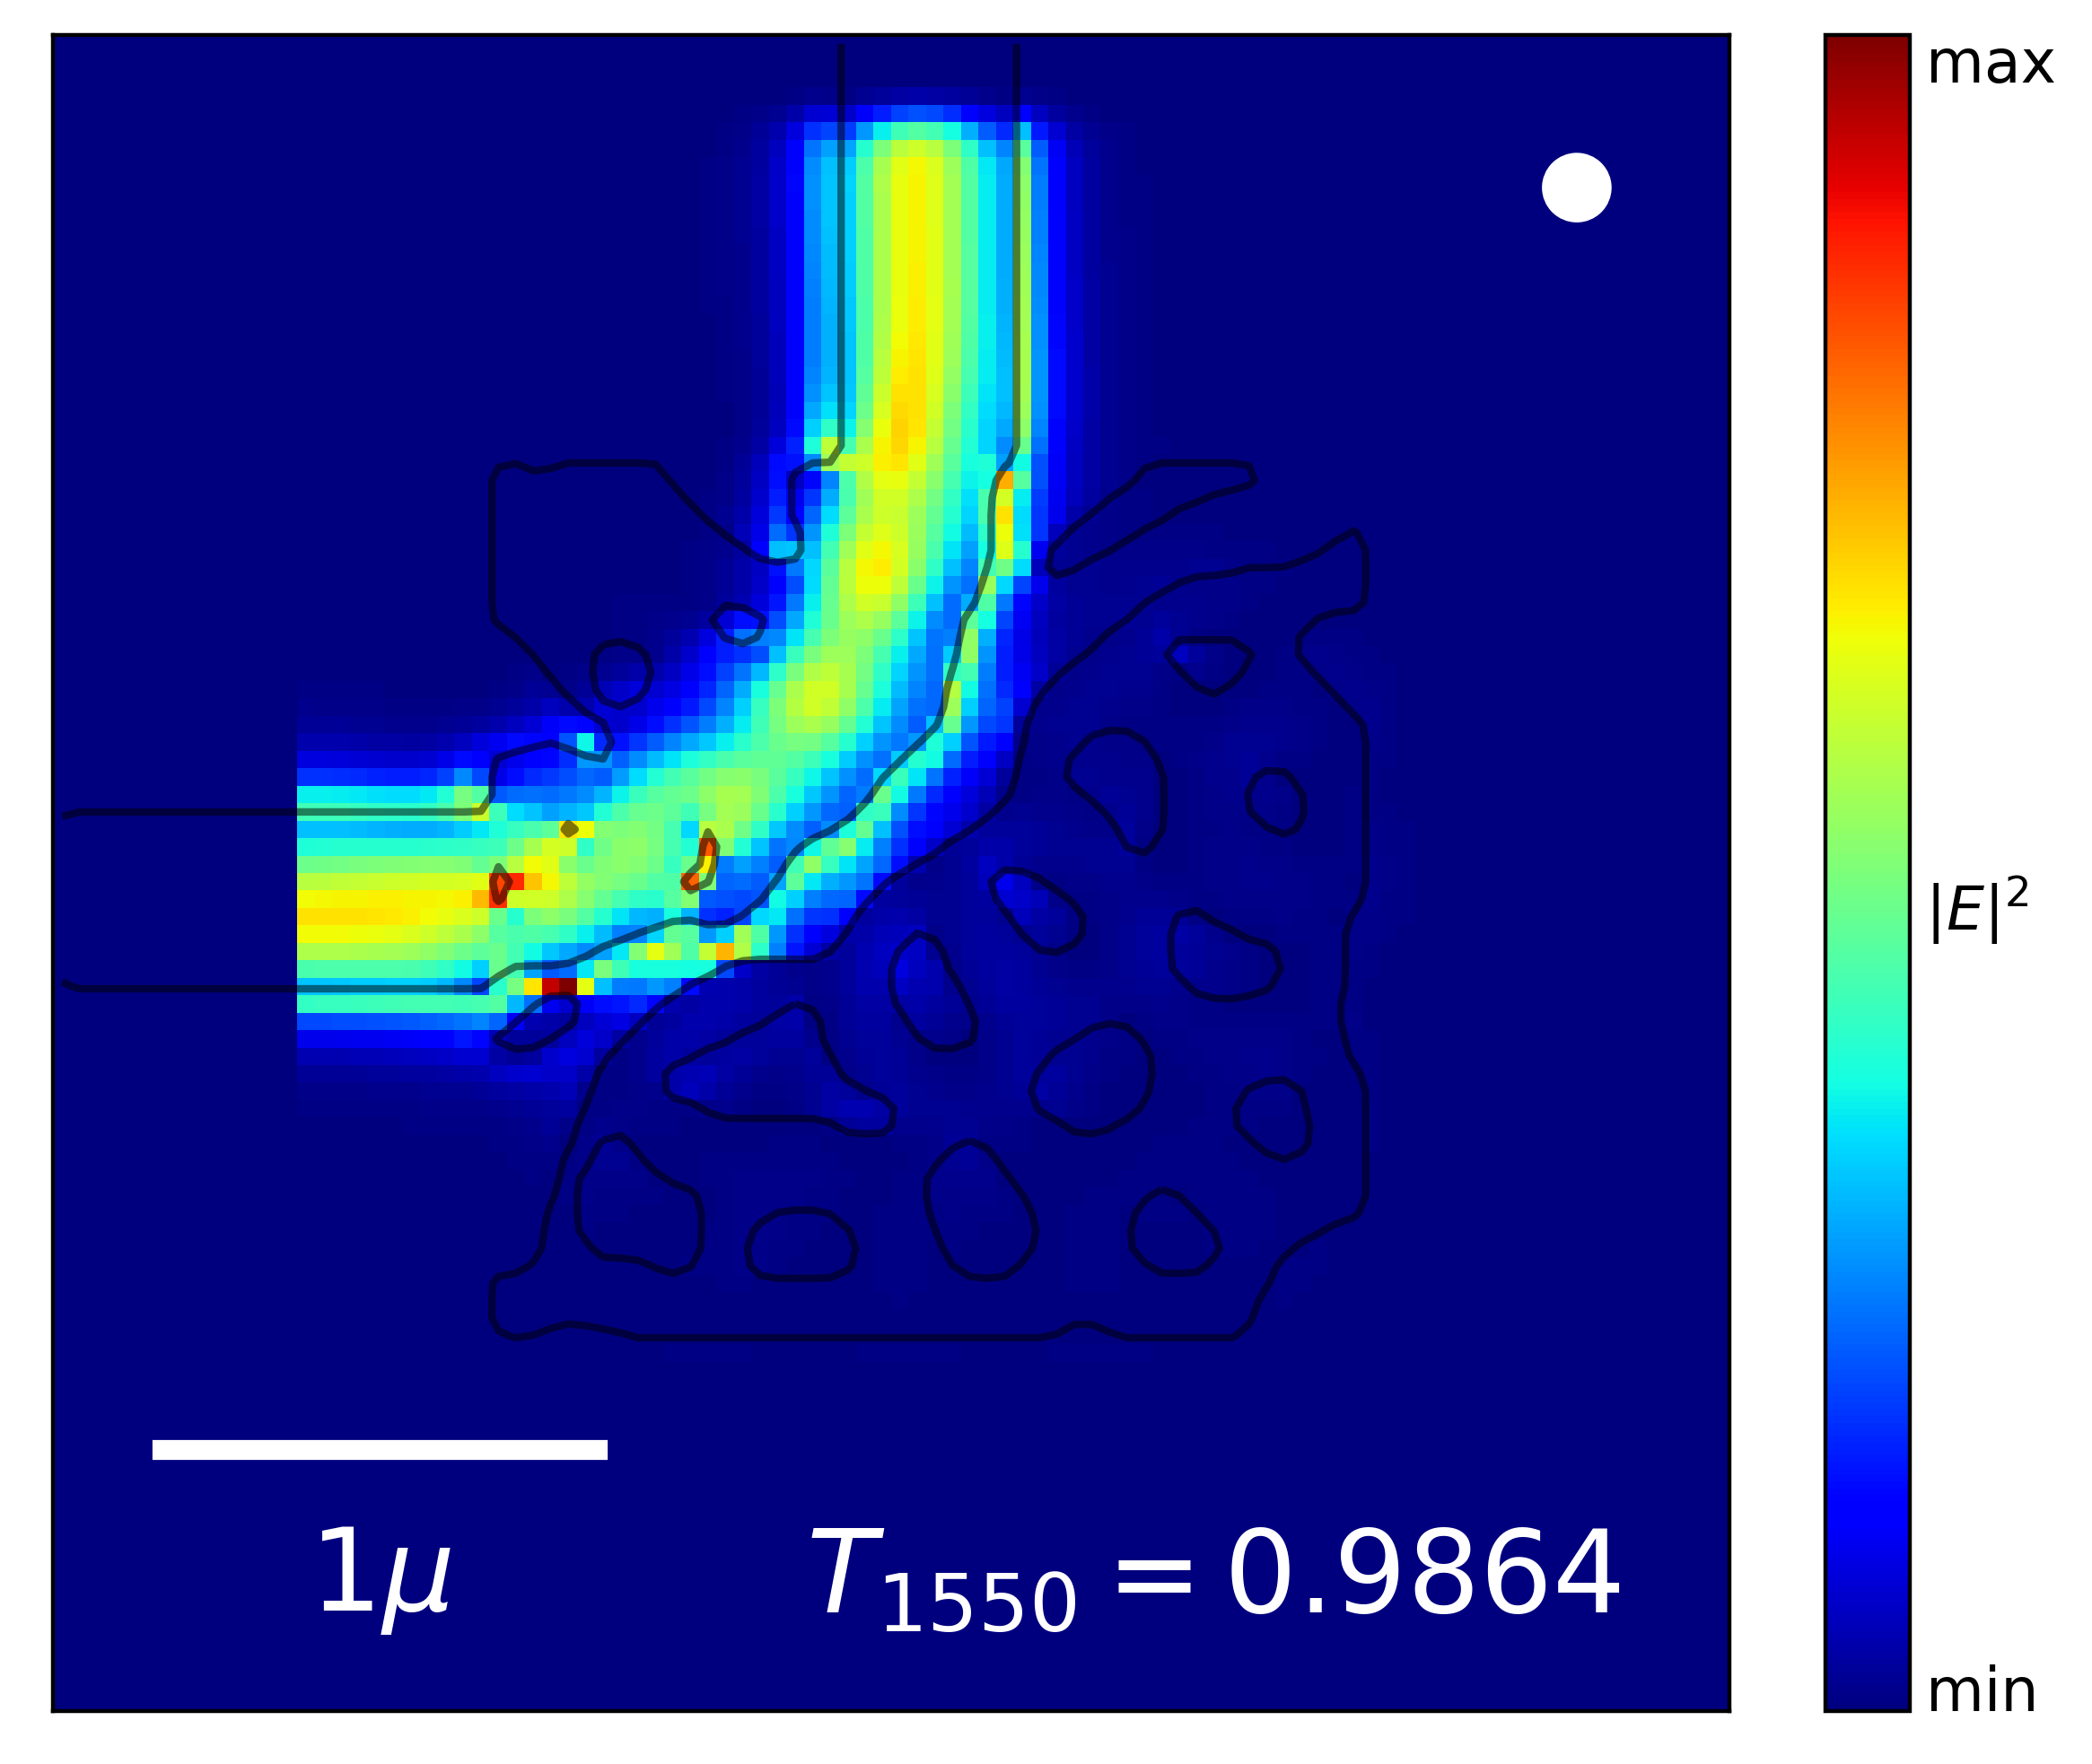
\includegraphics[width=0.33\textwidth]{image/results/bend/L-BFGS-B/visualize_field_fab_512.png} \\
    \hline
    \end{tabular}
    \hspace*{-3cm}
    \caption{Resultados de optimizar el \emph{bend} usando L-BFGS-B}
    \label{tab:opt-LBFGSB-bend}
\end{table}

% Bend - CMA-ES
\begin{table}[ht]
    \centering
    \vspace*{-2.5cm}
    \hspace*{-3cm}
    \begin{tabular}{|c|c|c|c|}
    \hline 
    \emph{Seed} & Opt. continua & Opt. discreta &  Opt. de fabricación \\
    \hline
      \multirow{2}{*}{128} &
      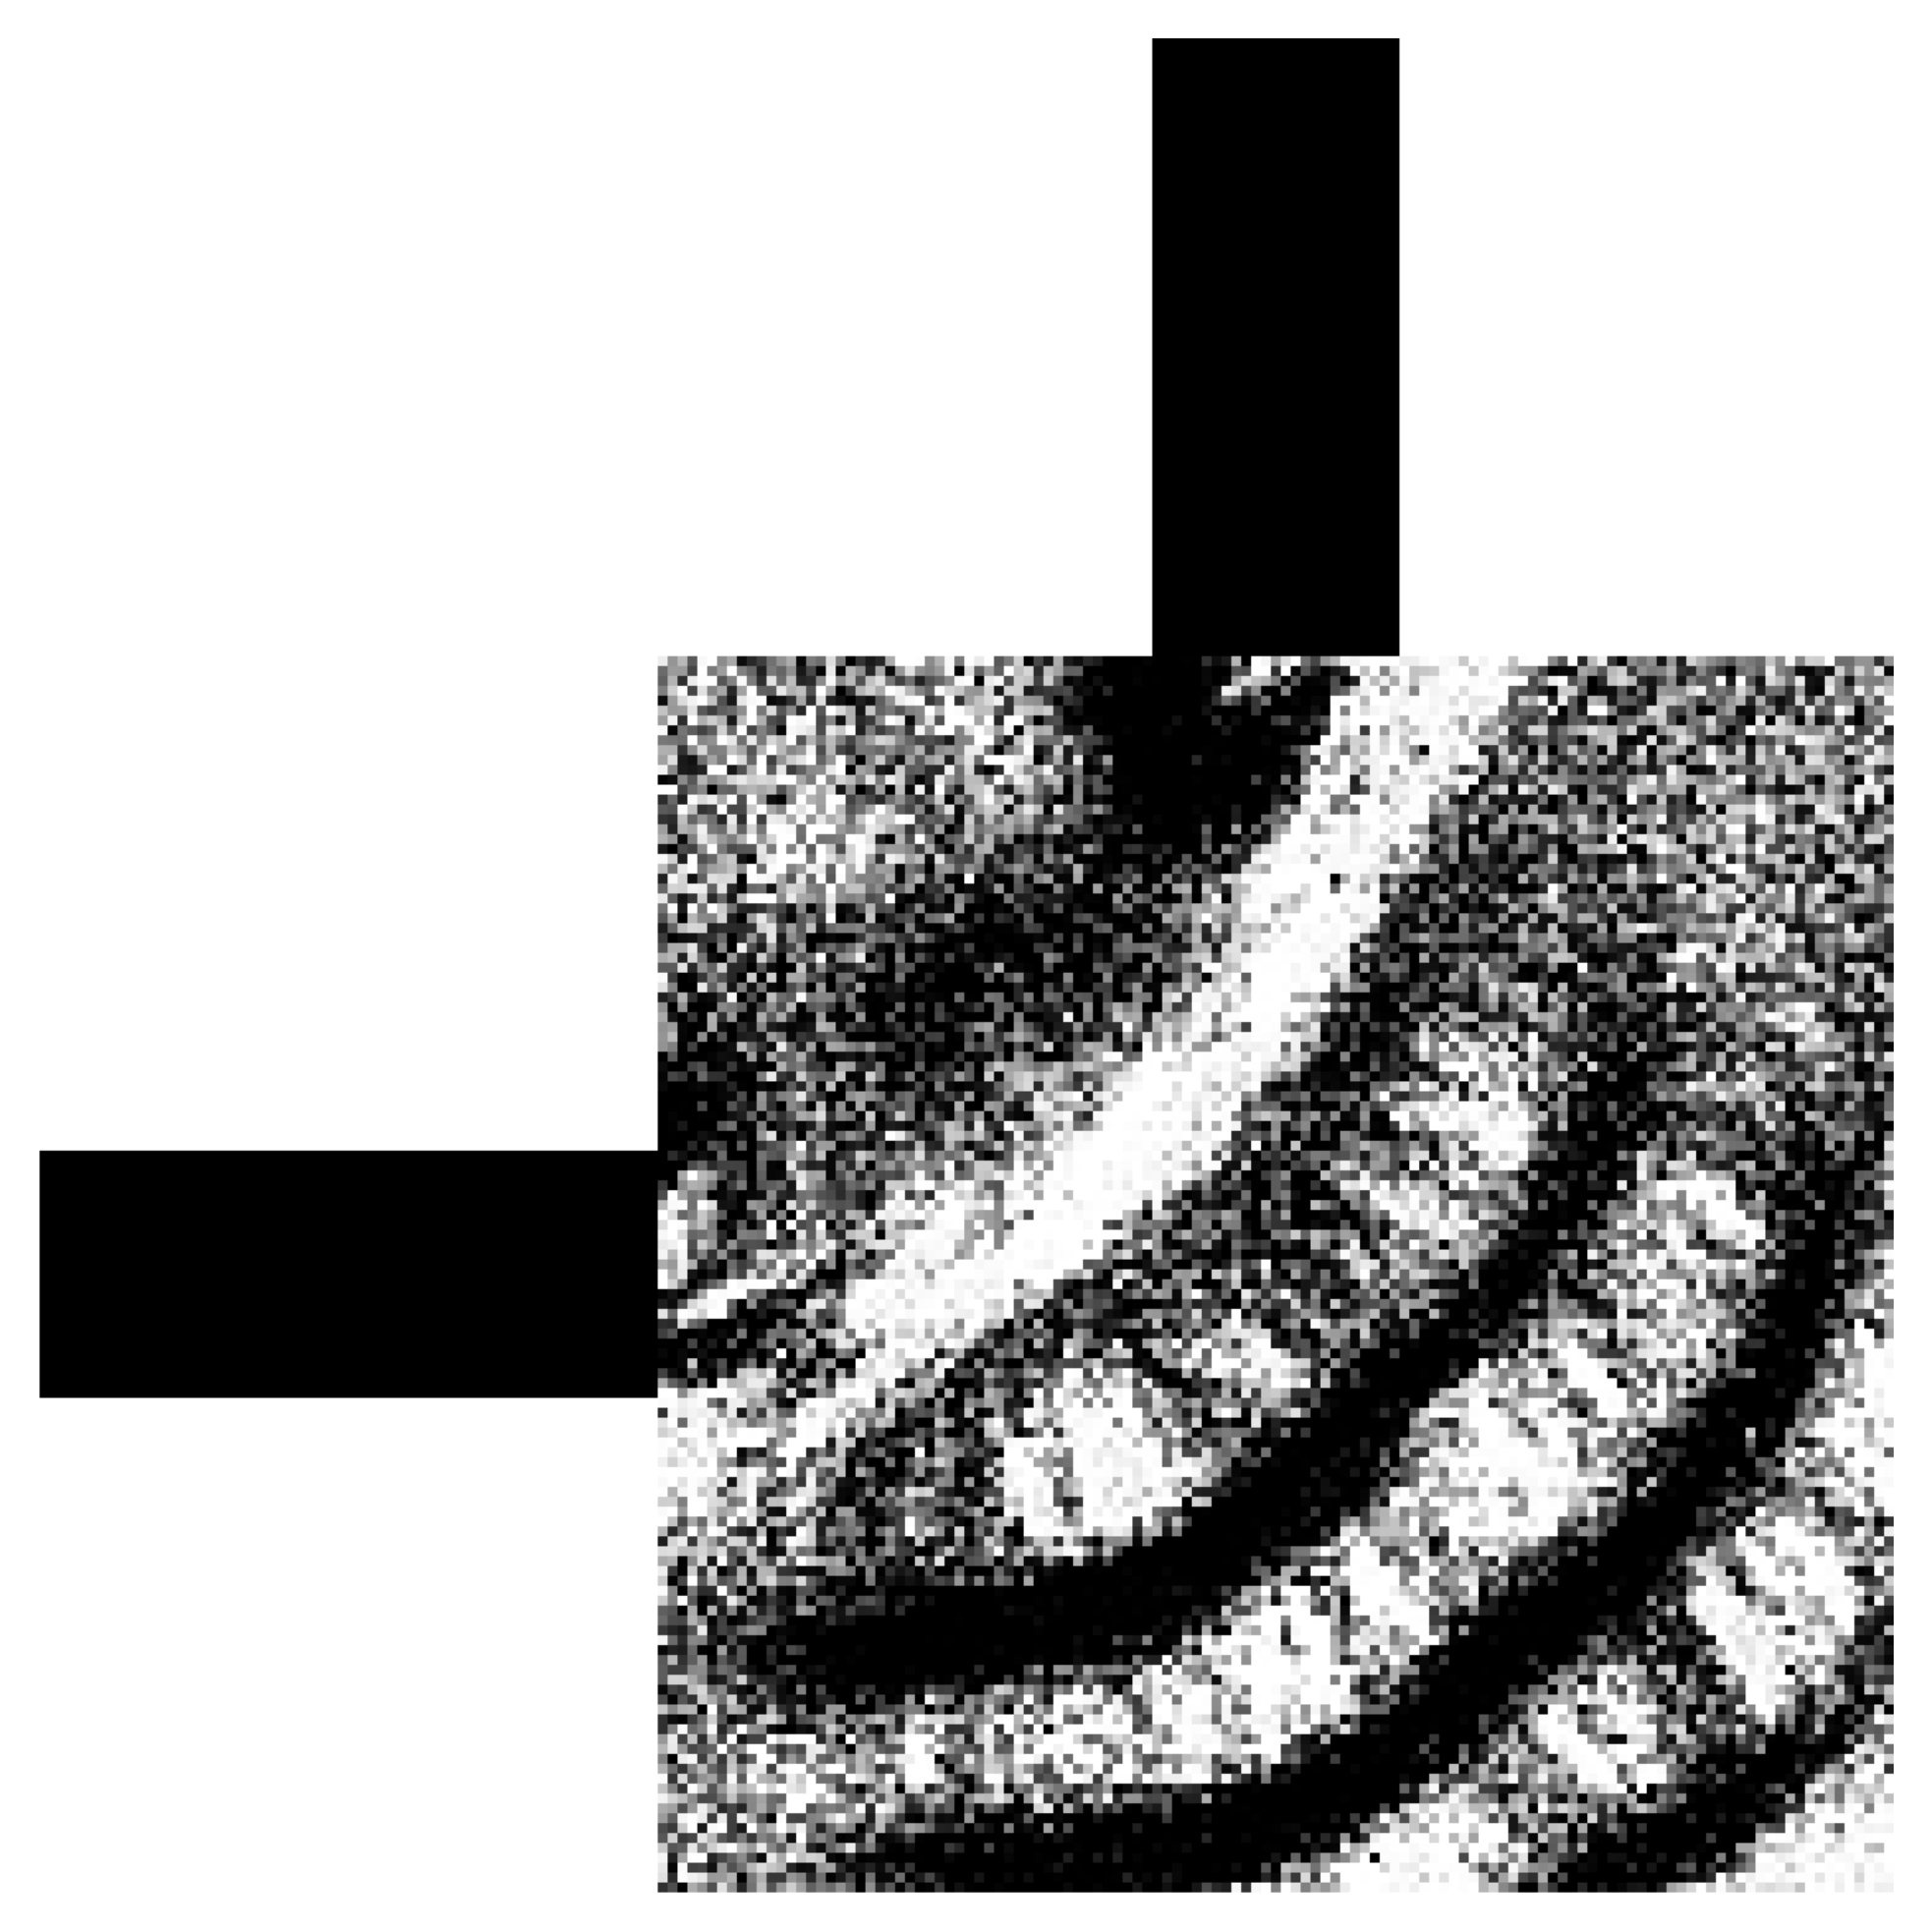
\includegraphics[width=0.20\textwidth]{image/results/bend/CMA-ES/visualize_eps_cont_128.png} &
      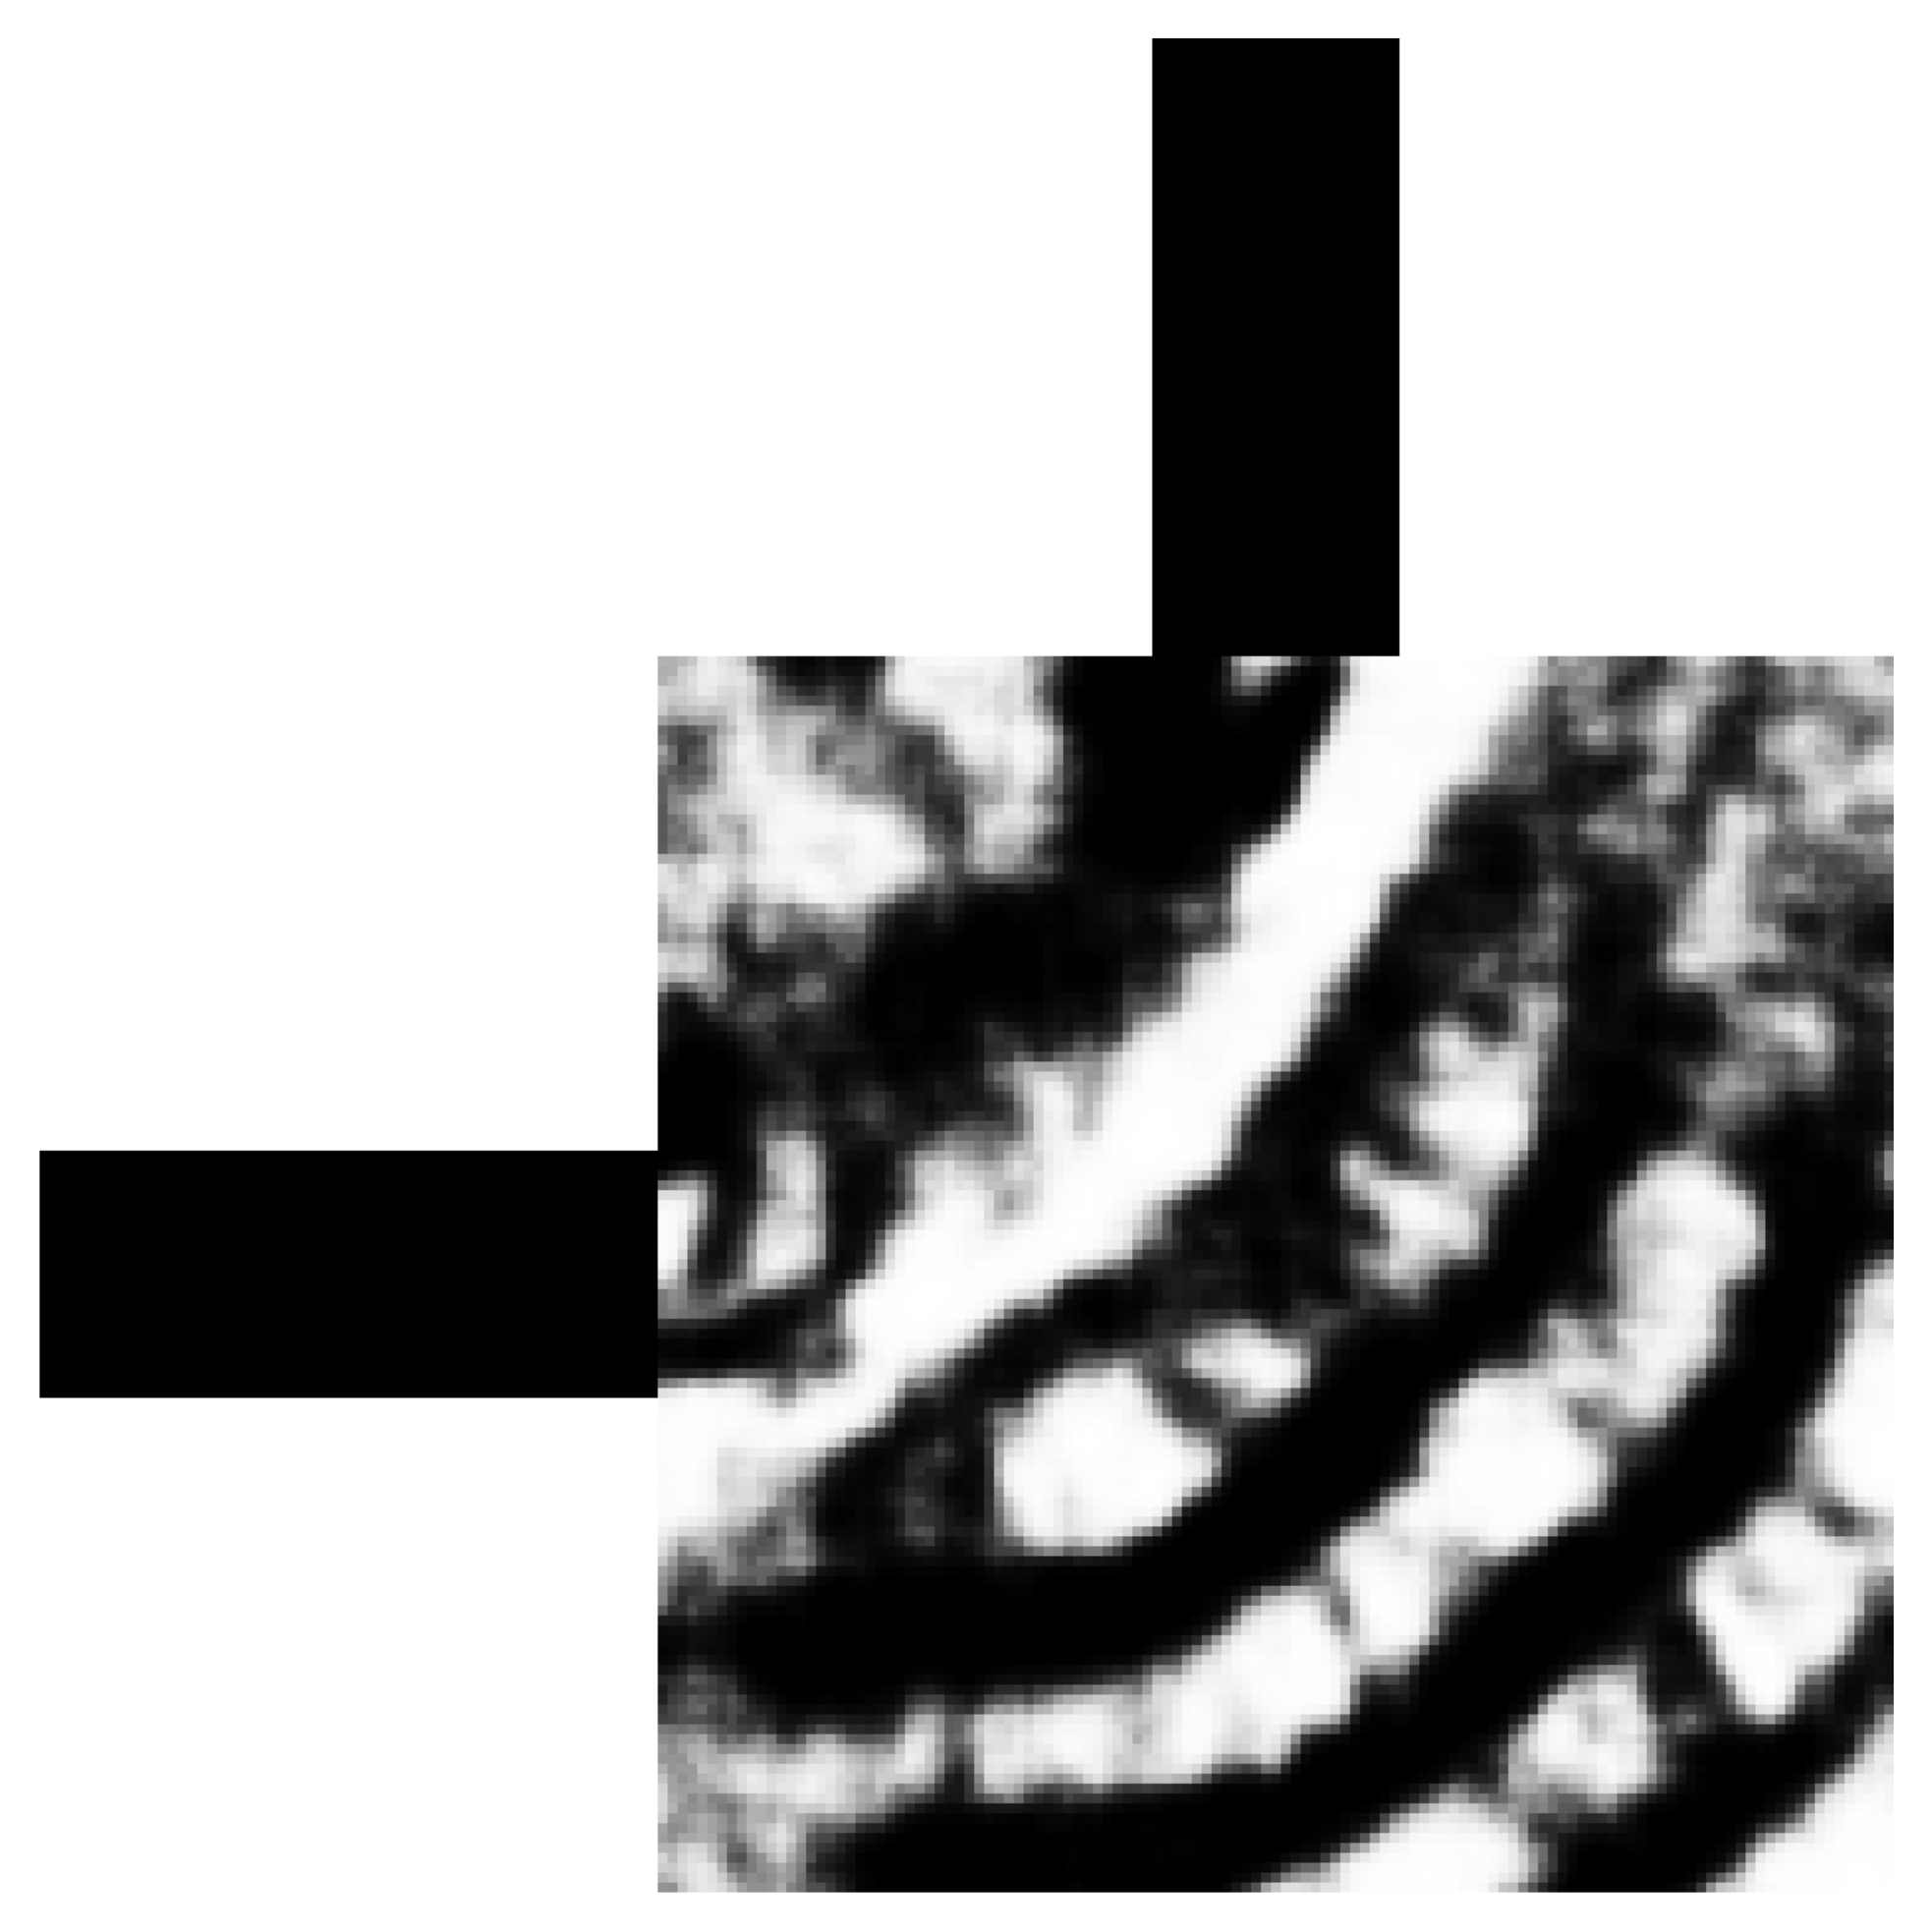
\includegraphics[width=0.20\textwidth]{image/results/bend/CMA-ES/visualize_eps_disc_128.png} &
      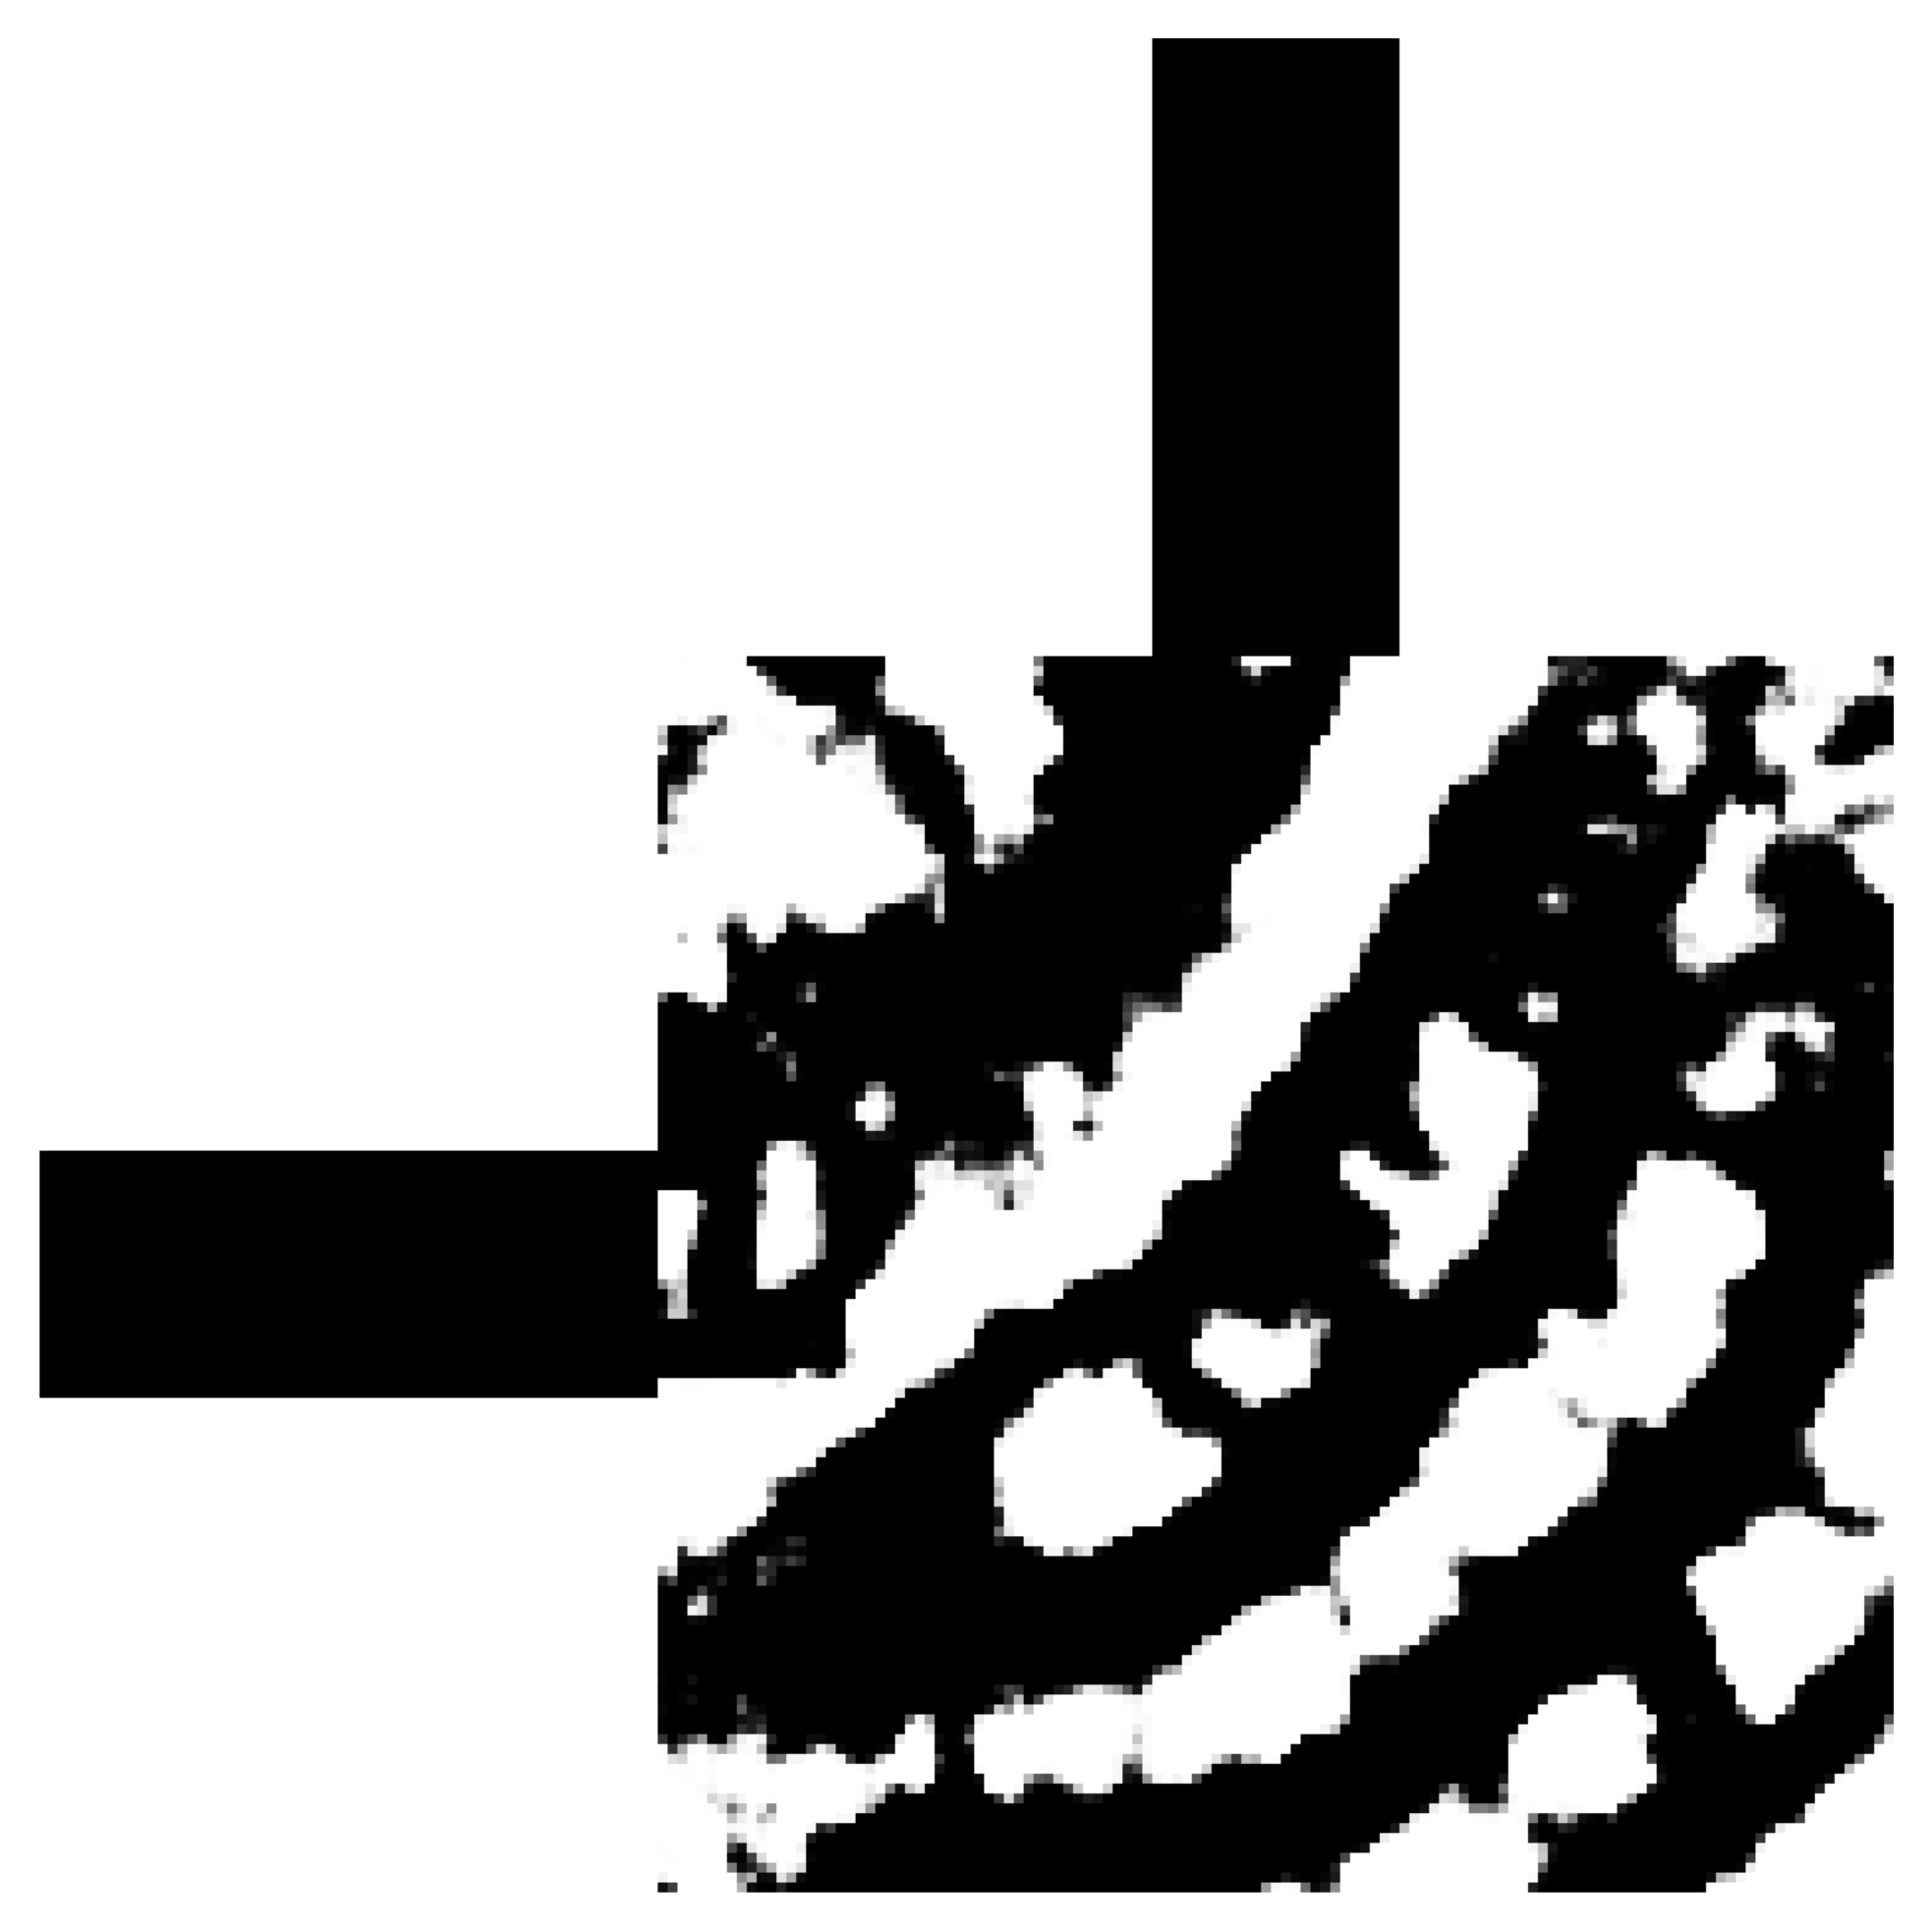
\includegraphics[width=0.20\textwidth]{image/results/bend/CMA-ES/visualize_eps_fab_128.png} \\
      \cline{2-4}
      &
      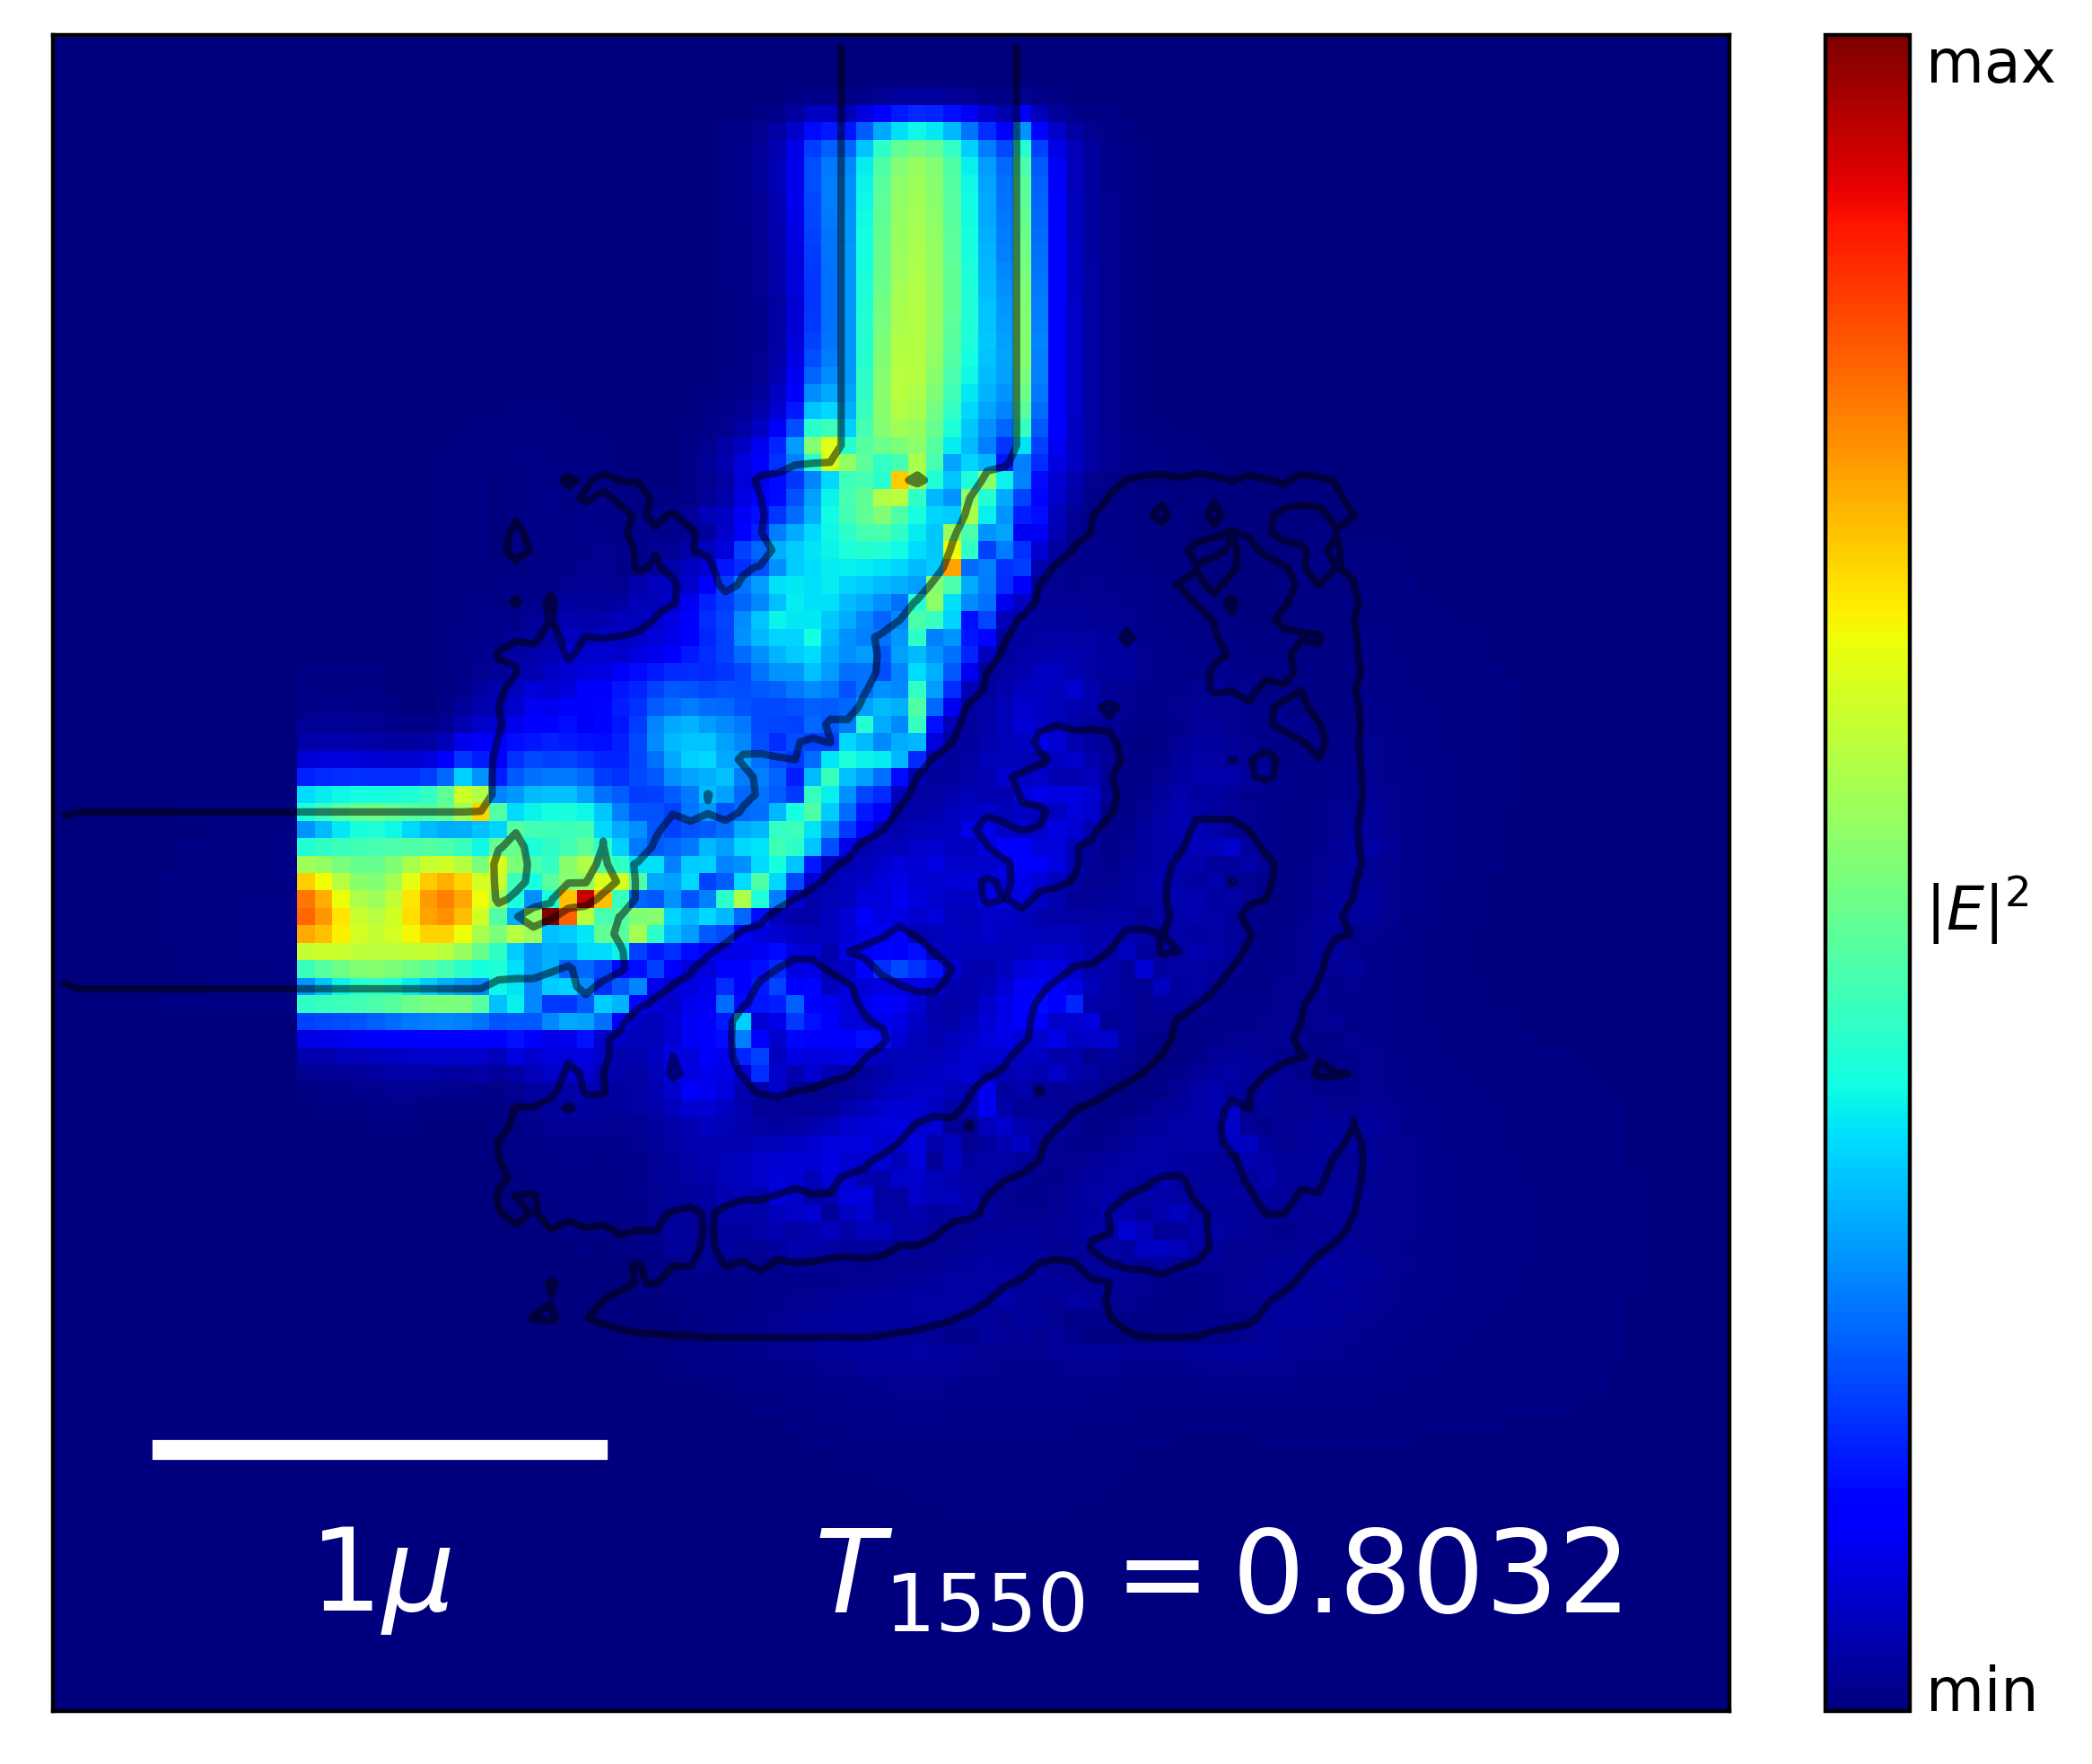
\includegraphics[width=0.33\textwidth]{image/results/bend/CMA-ES/visualize_field_cont_128.png} &
      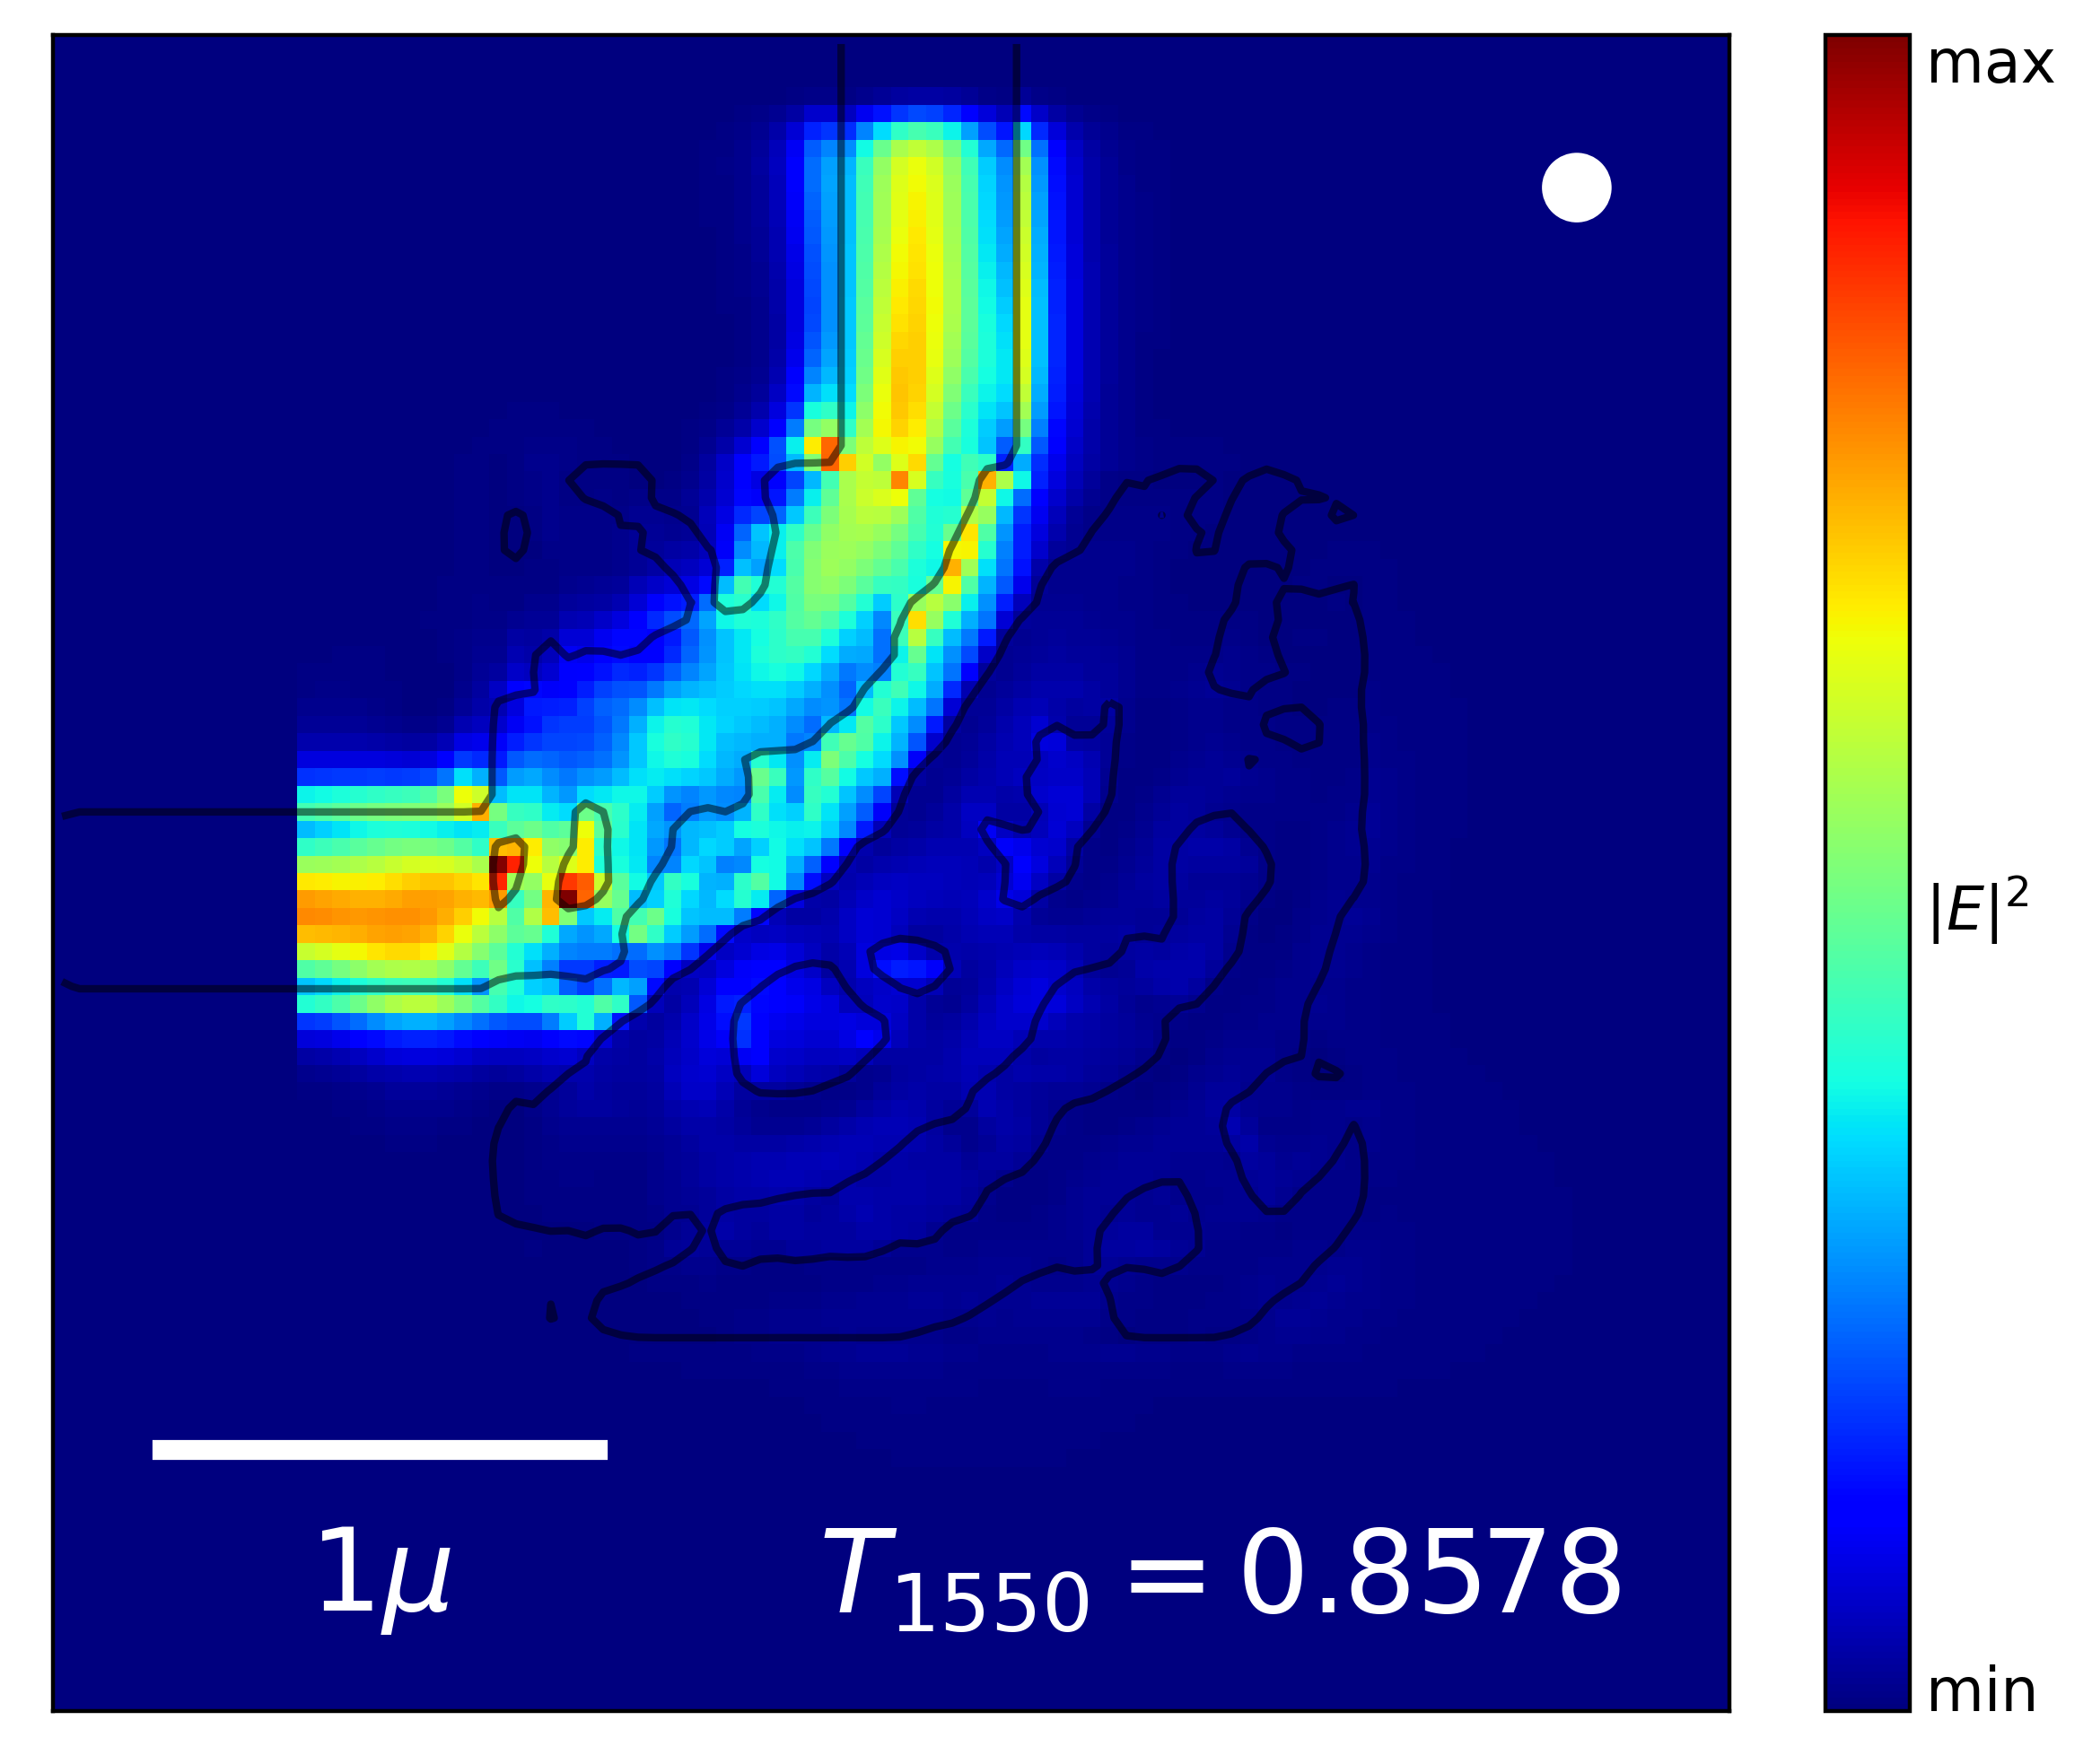
\includegraphics[width=0.33\textwidth]{image/results/bend/CMA-ES/visualize_field_disc_128.png} &
      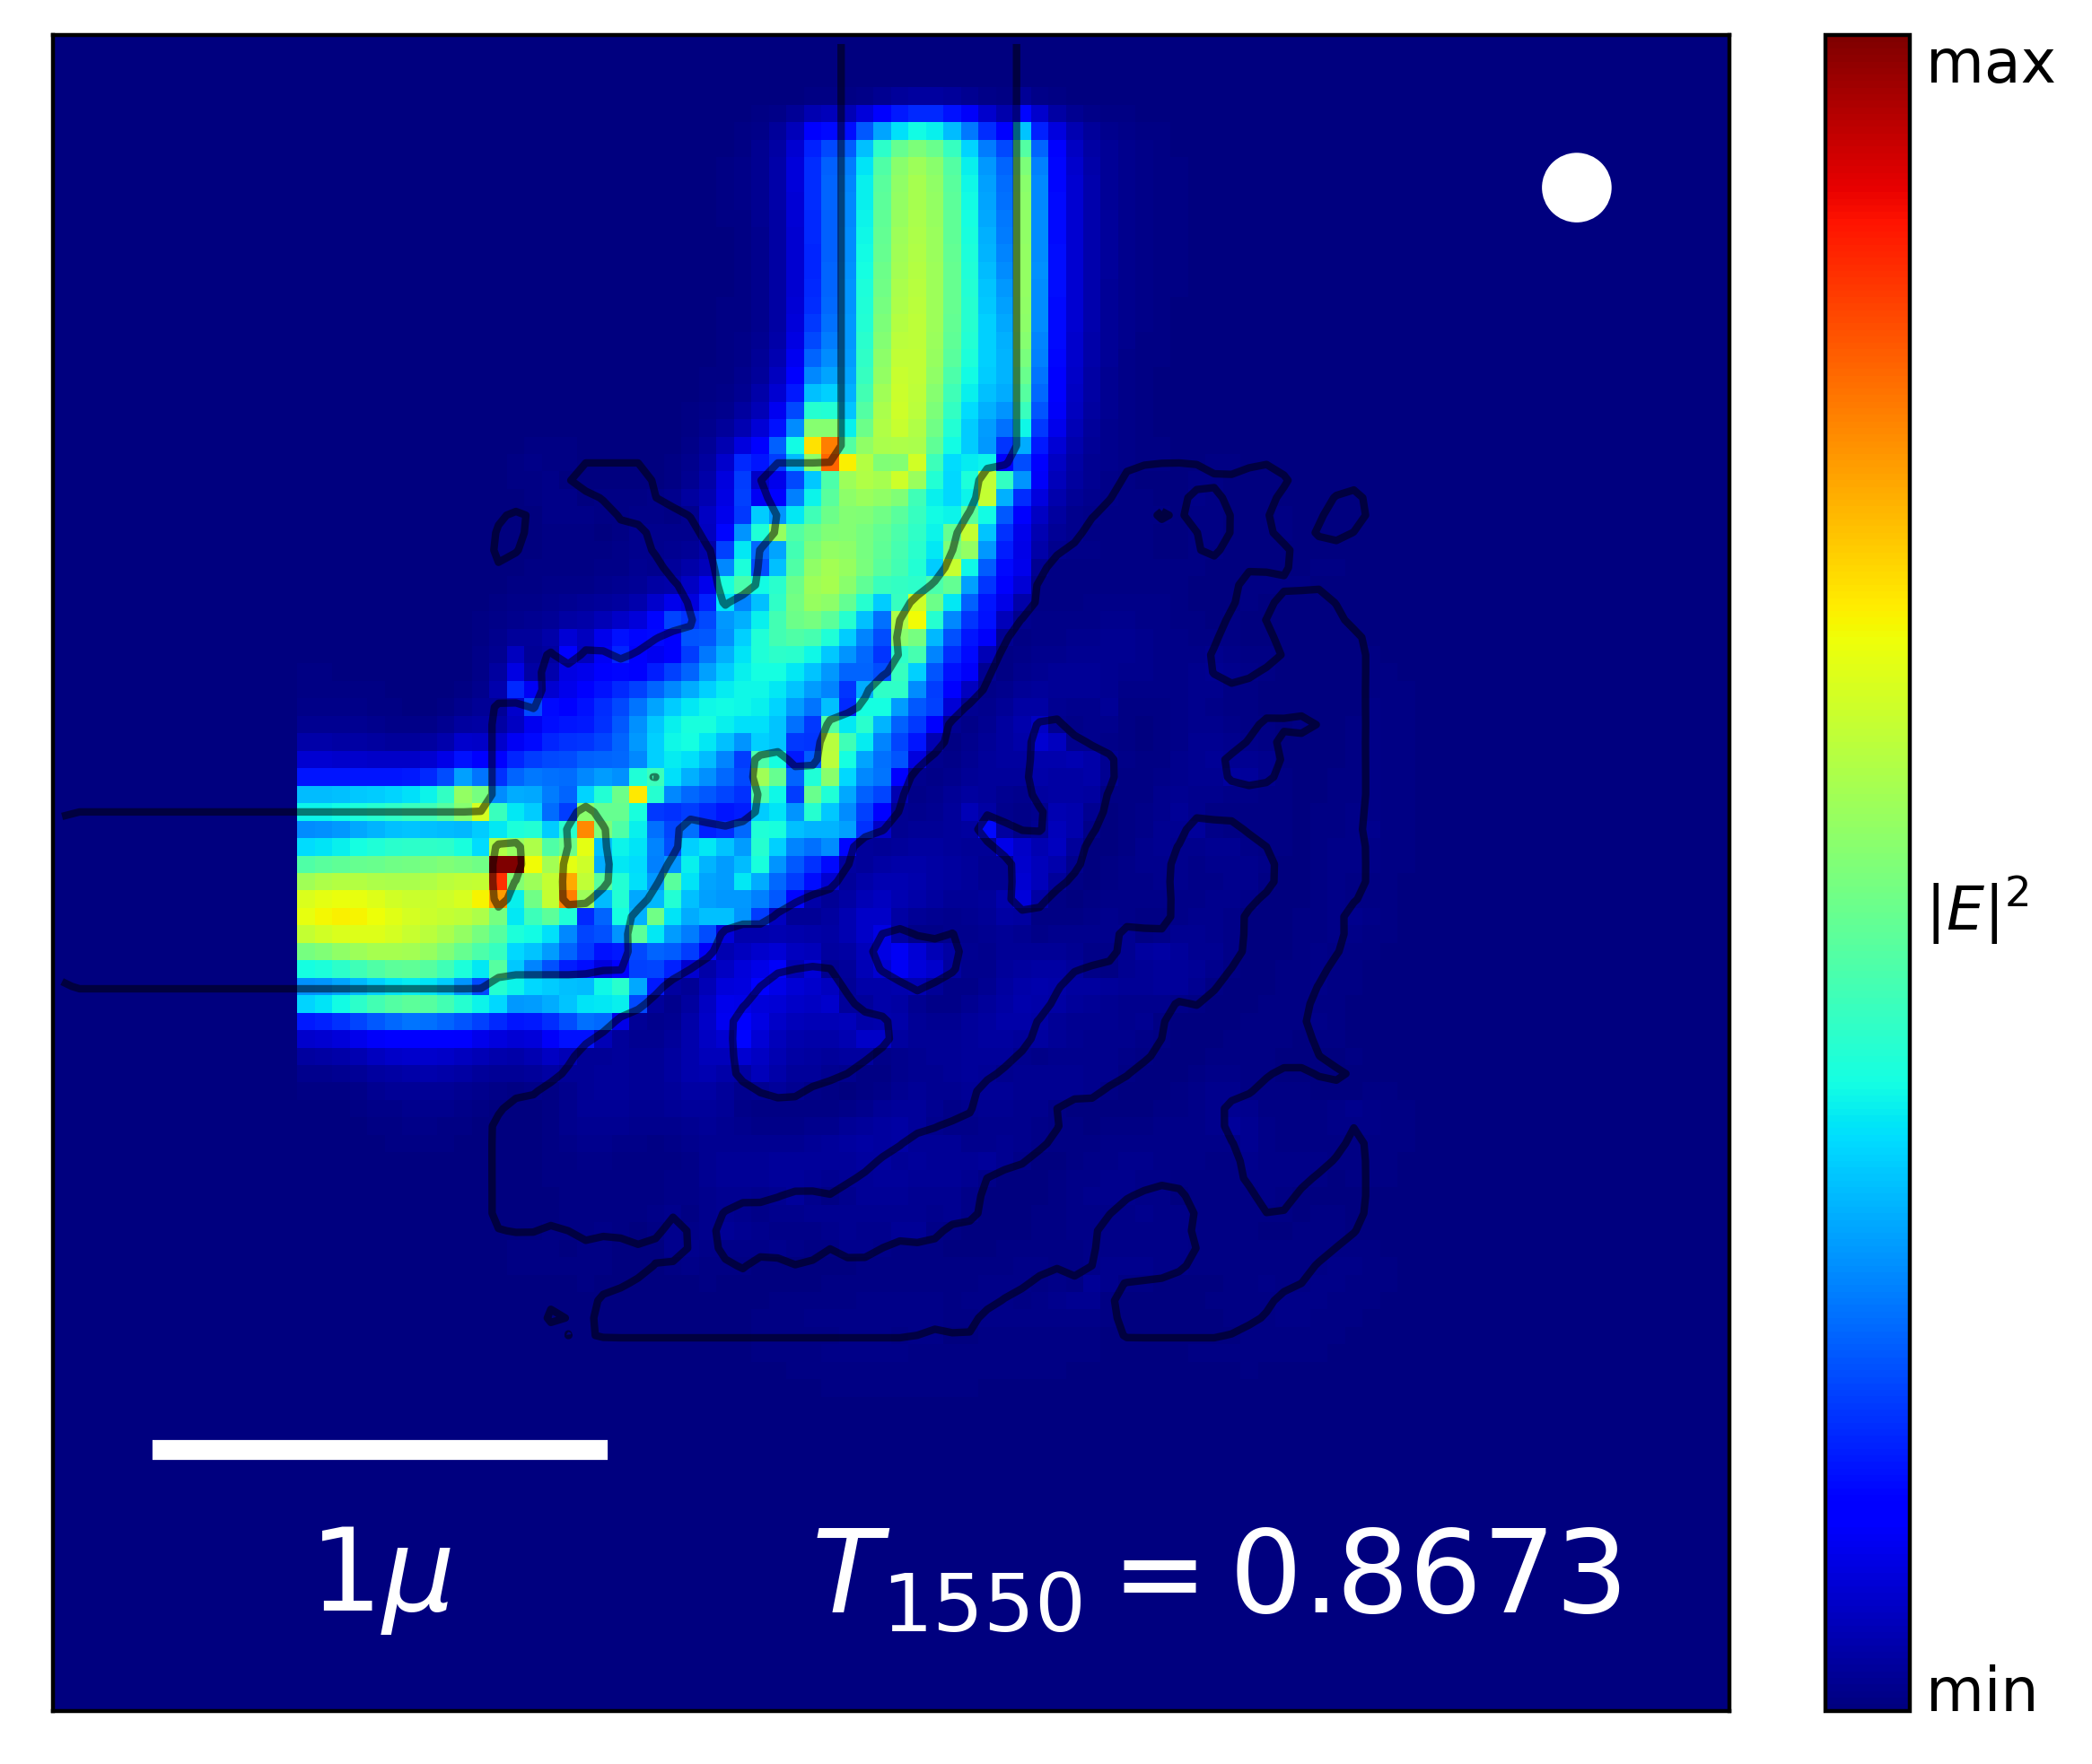
\includegraphics[width=0.33\textwidth]{image/results/bend/CMA-ES/visualize_field_fab_128.png} \\
    \hline
      \multirow{2}{*}{256} &
      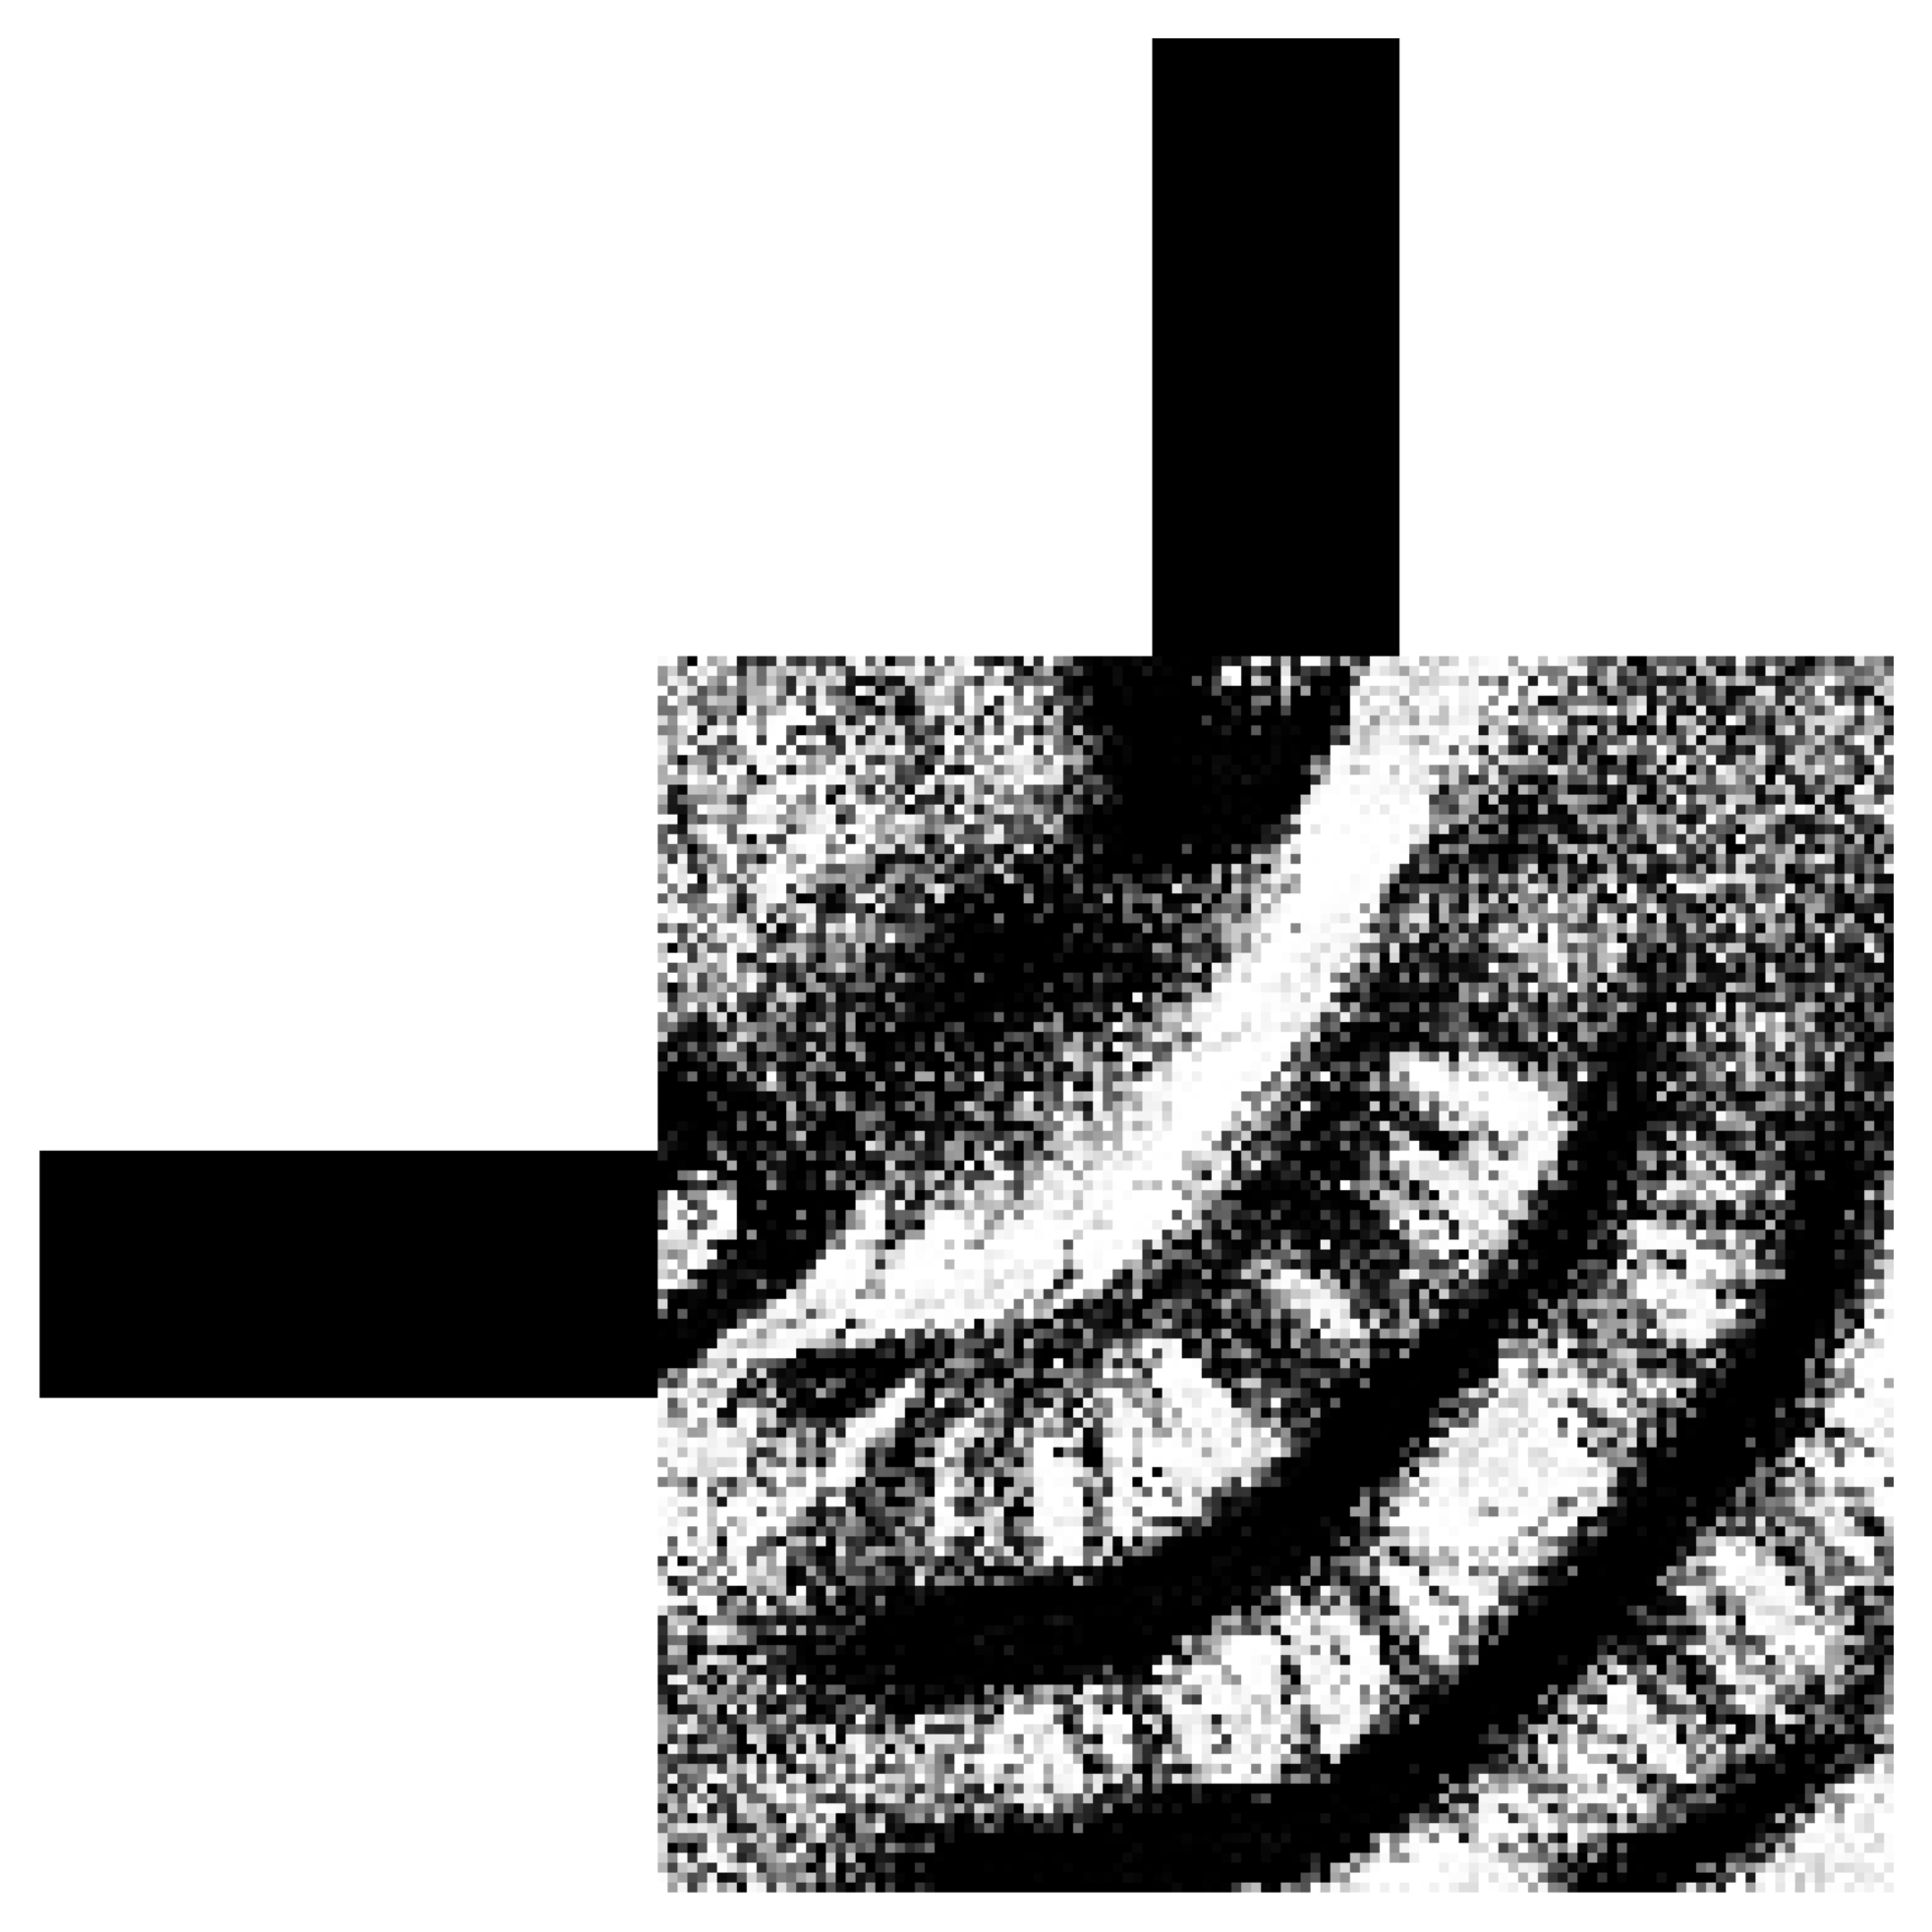
\includegraphics[width=0.20\textwidth]{image/results/bend/CMA-ES/visualize_eps_cont_256.png} &
      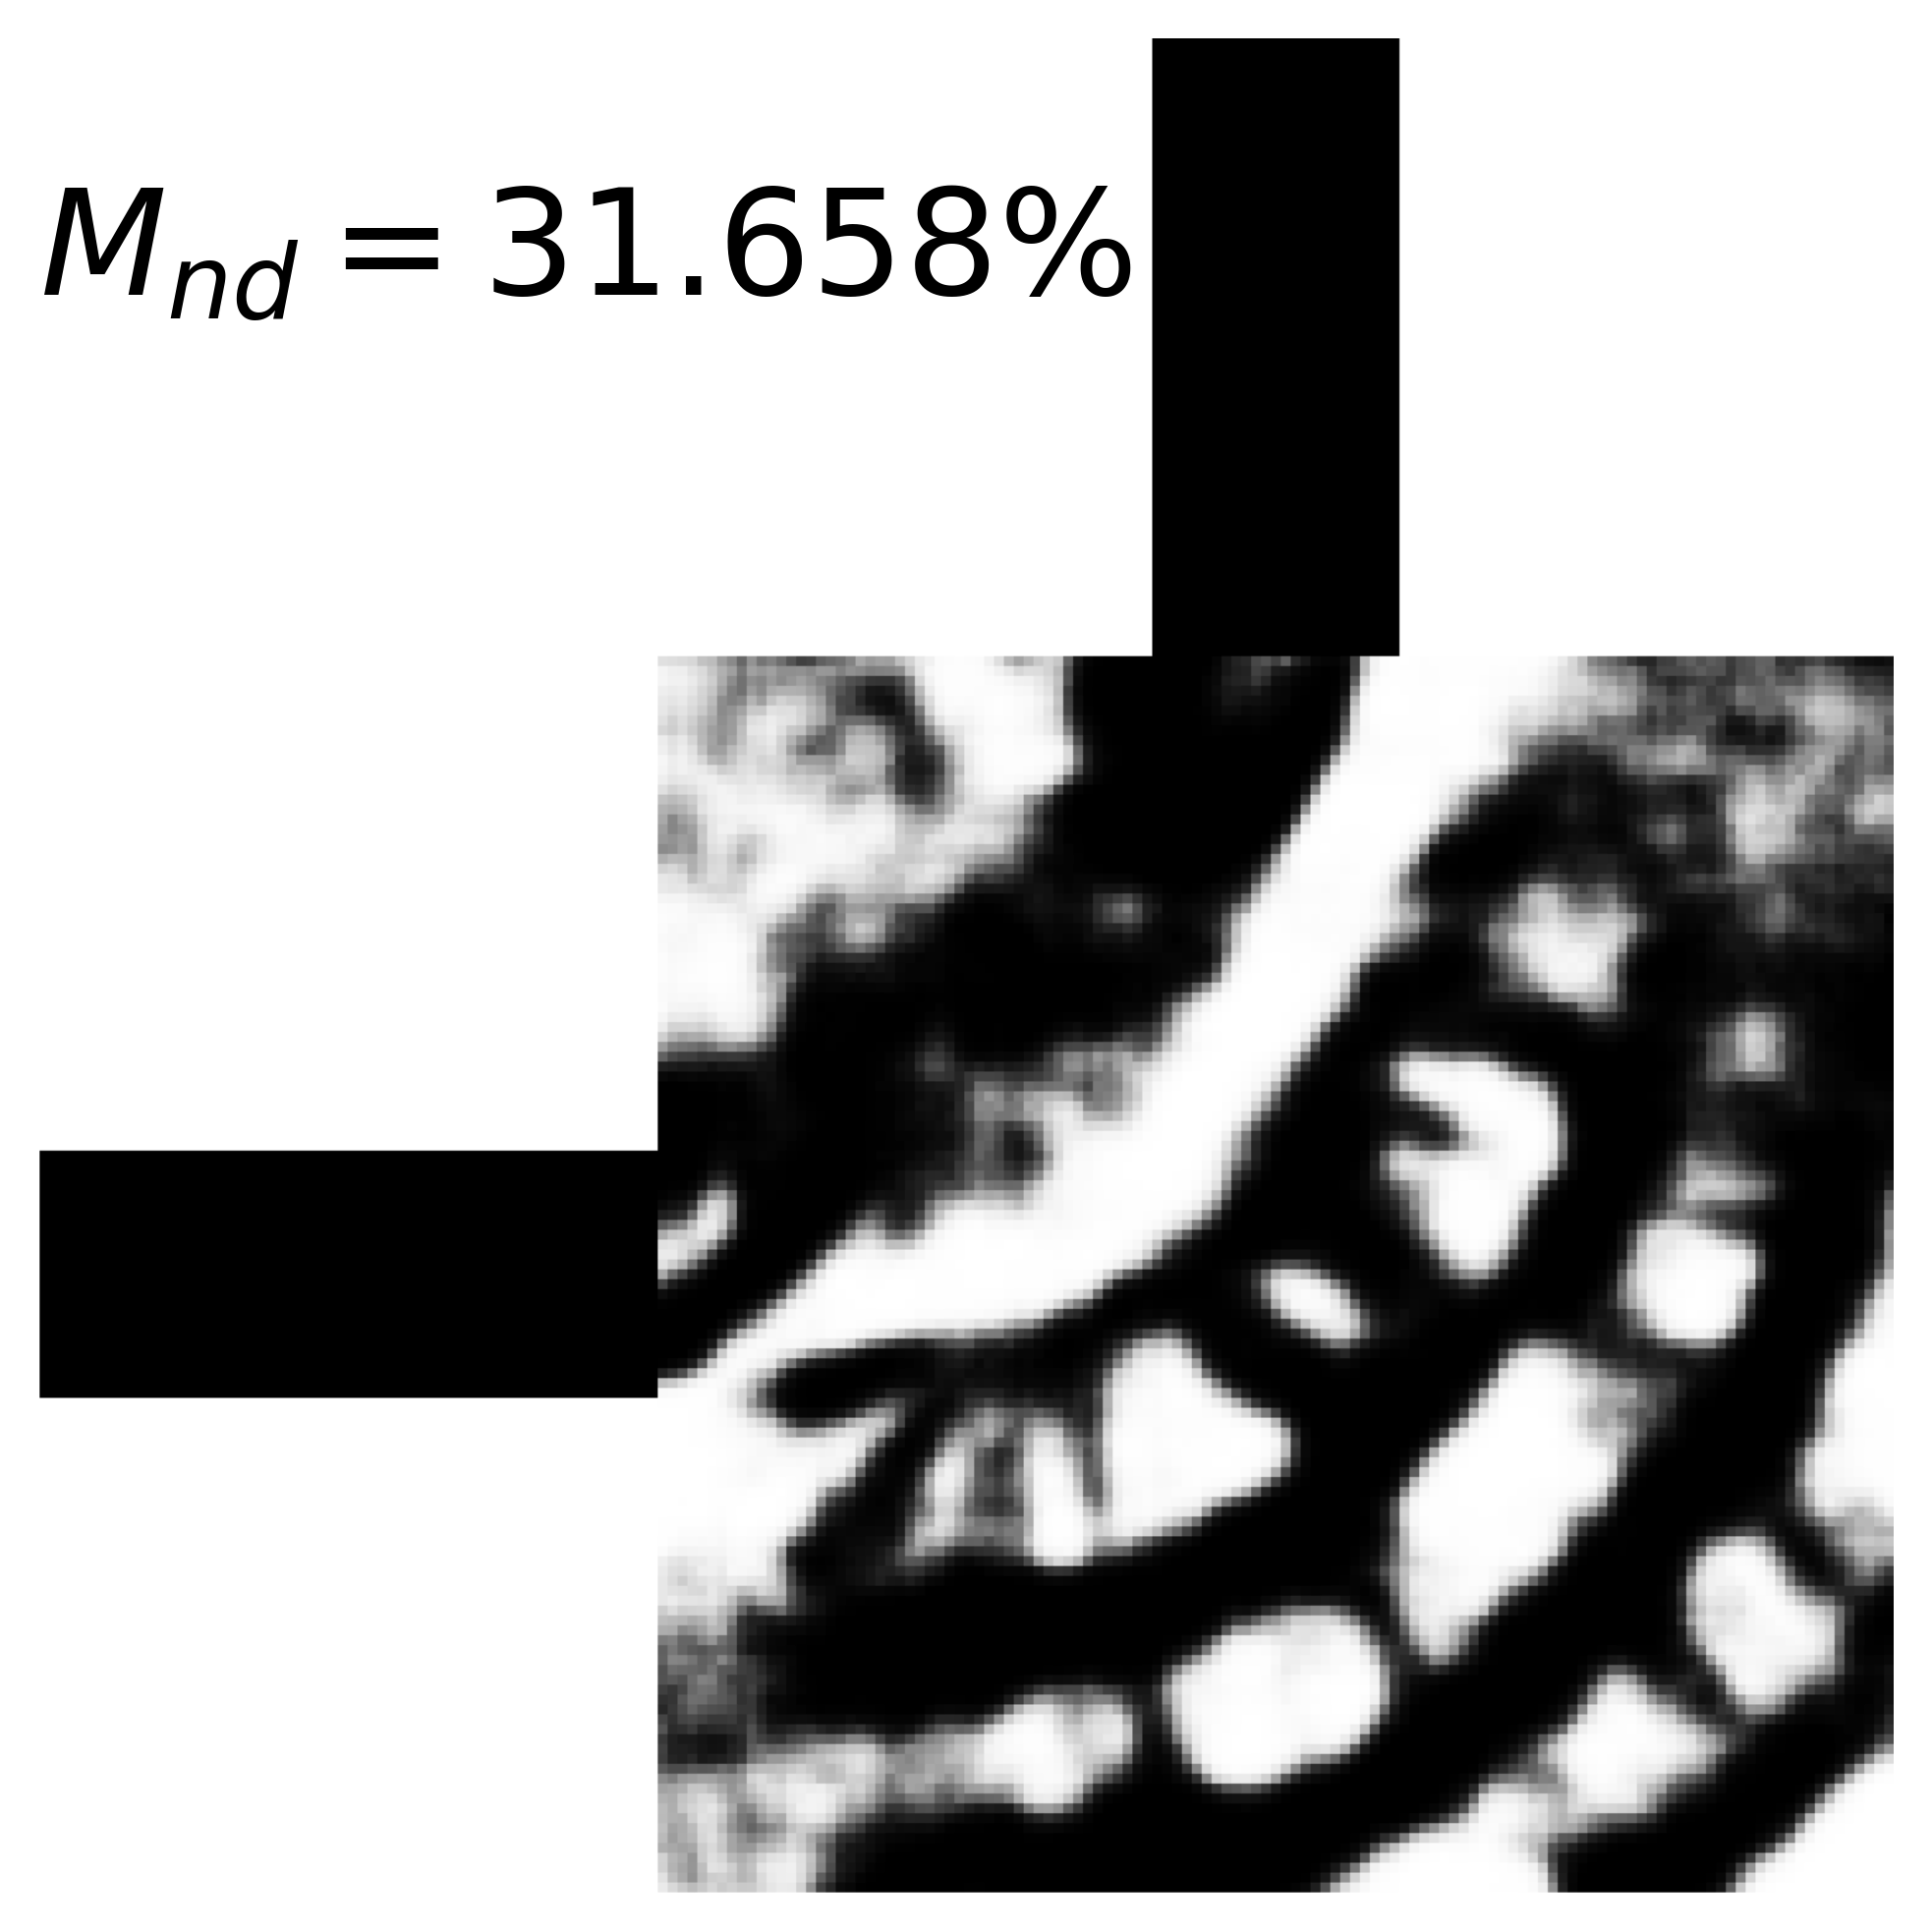
\includegraphics[width=0.20\textwidth]{image/results/bend/CMA-ES/visualize_eps_disc_256.png} &
      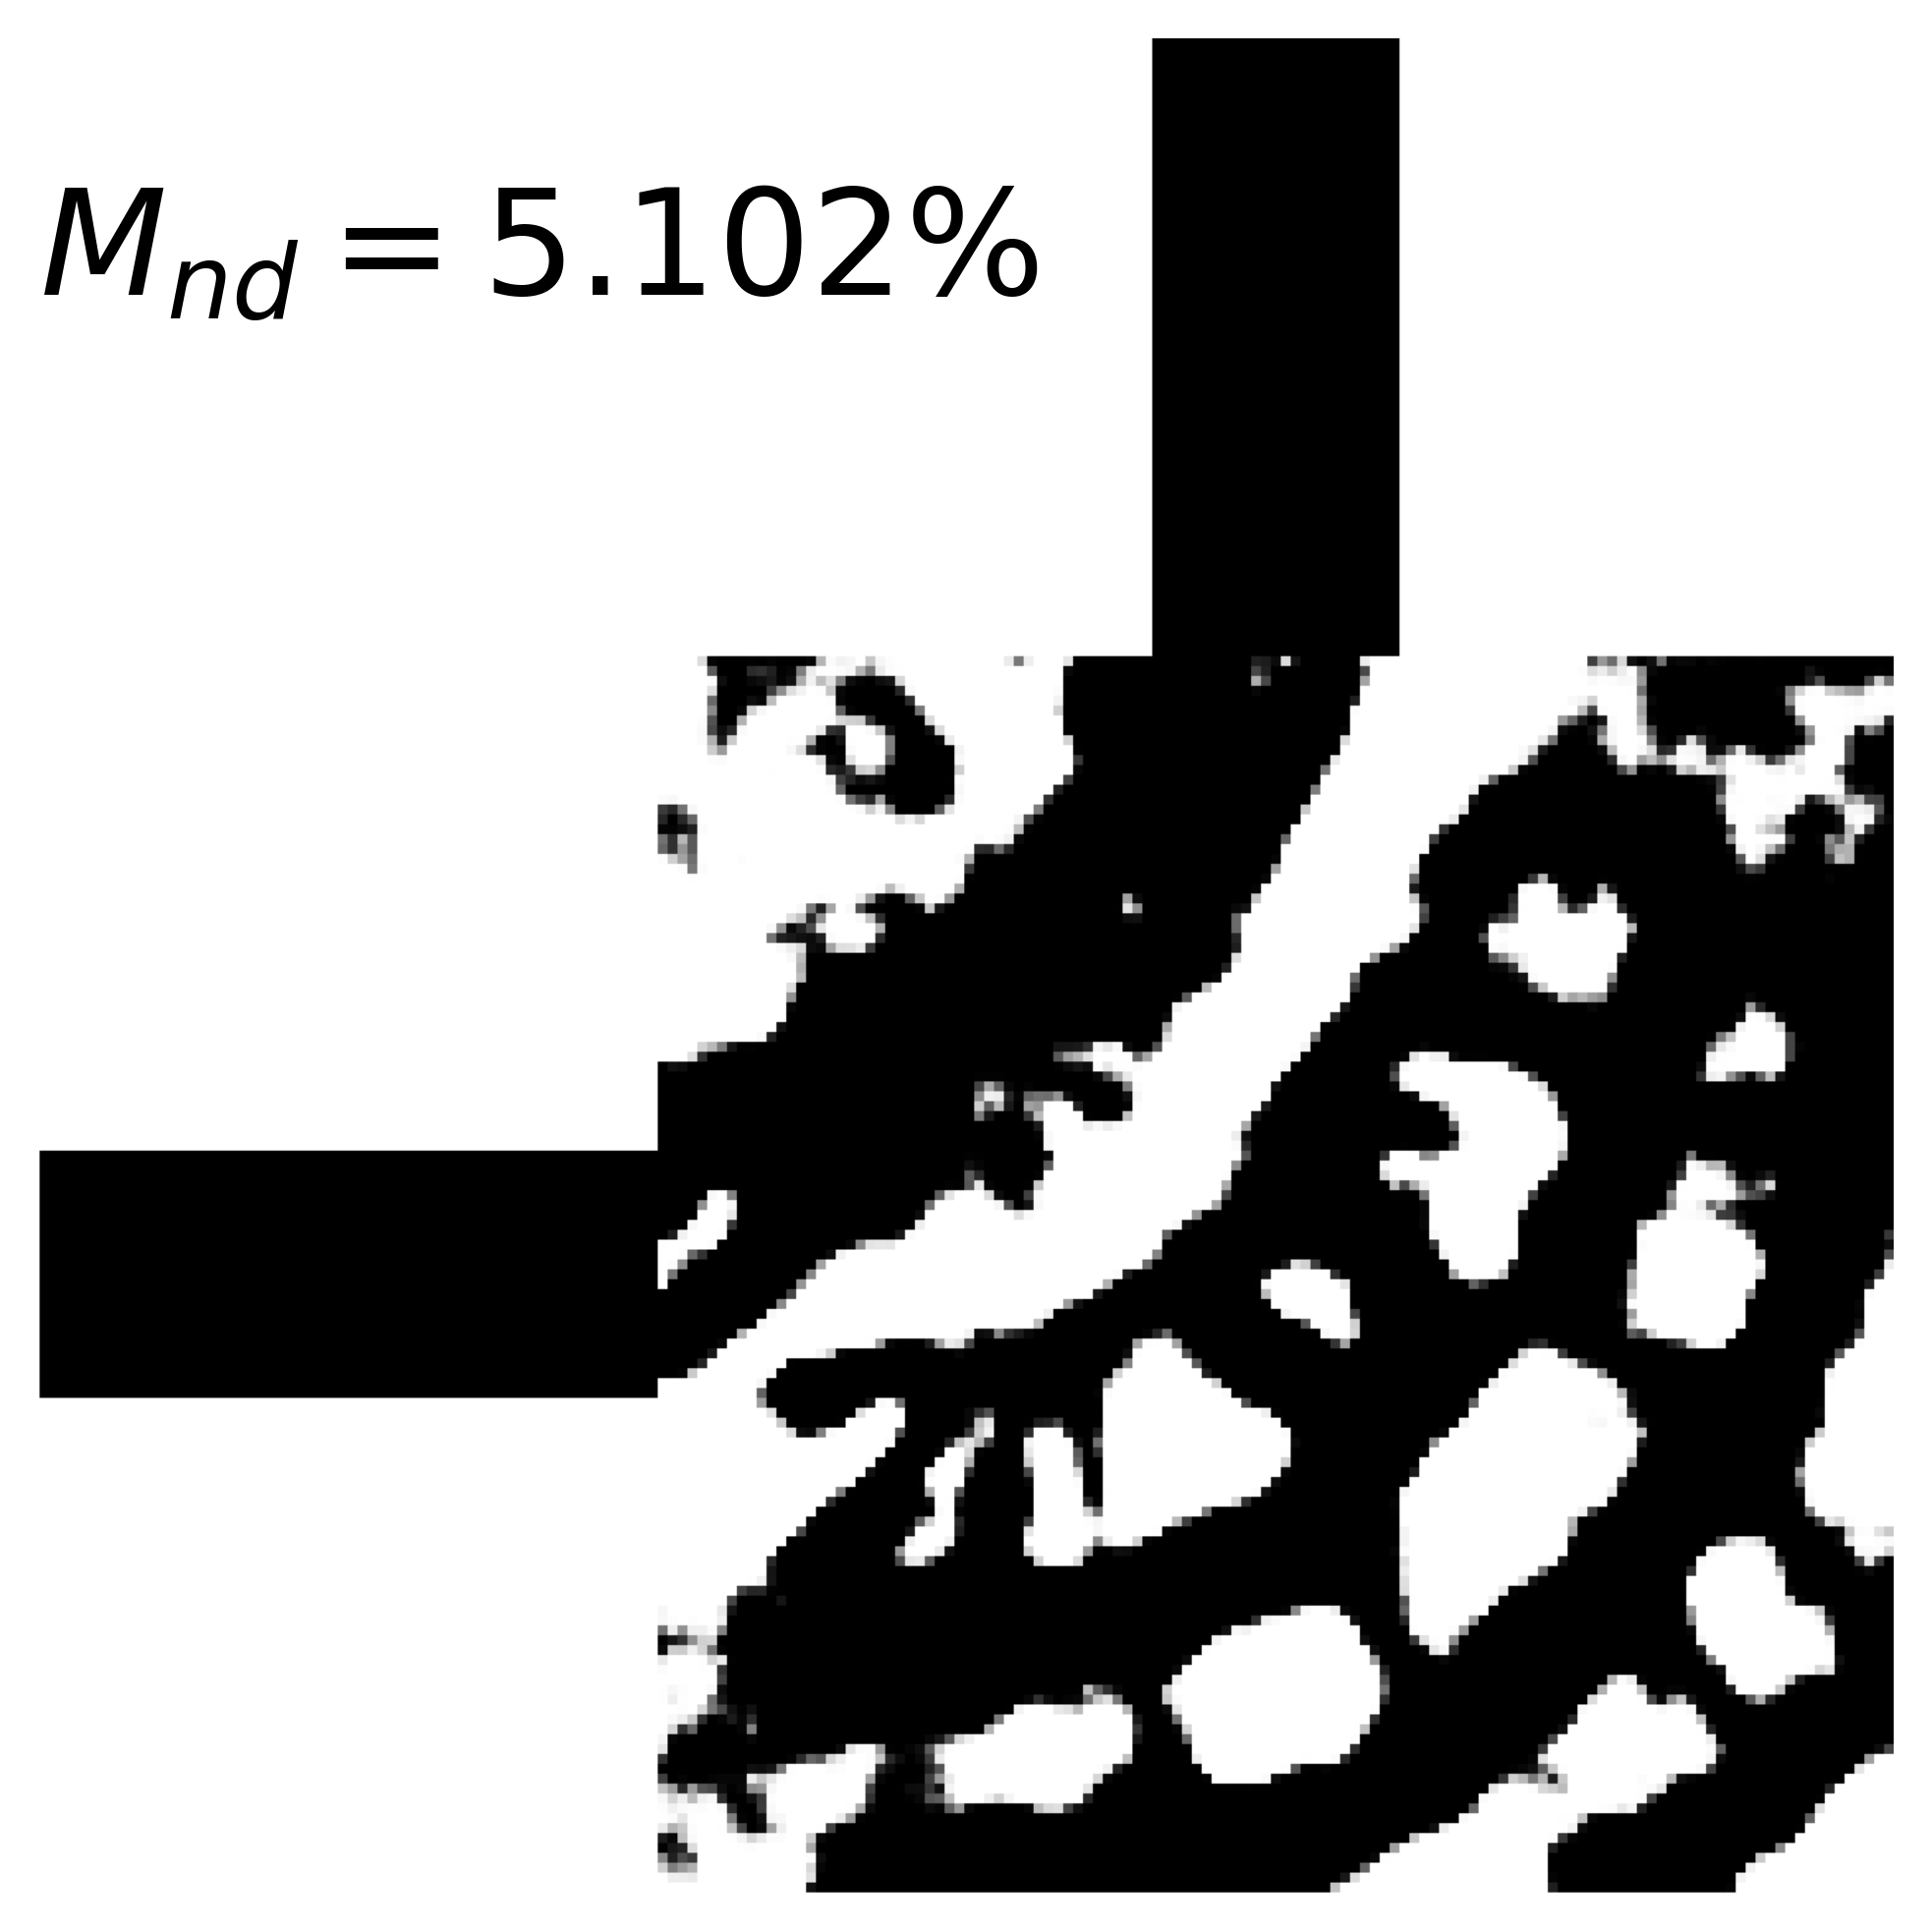
\includegraphics[width=0.20\textwidth]{image/results/bend/CMA-ES/visualize_eps_fab_256.png} \\
      \cline{2-4}
      &
      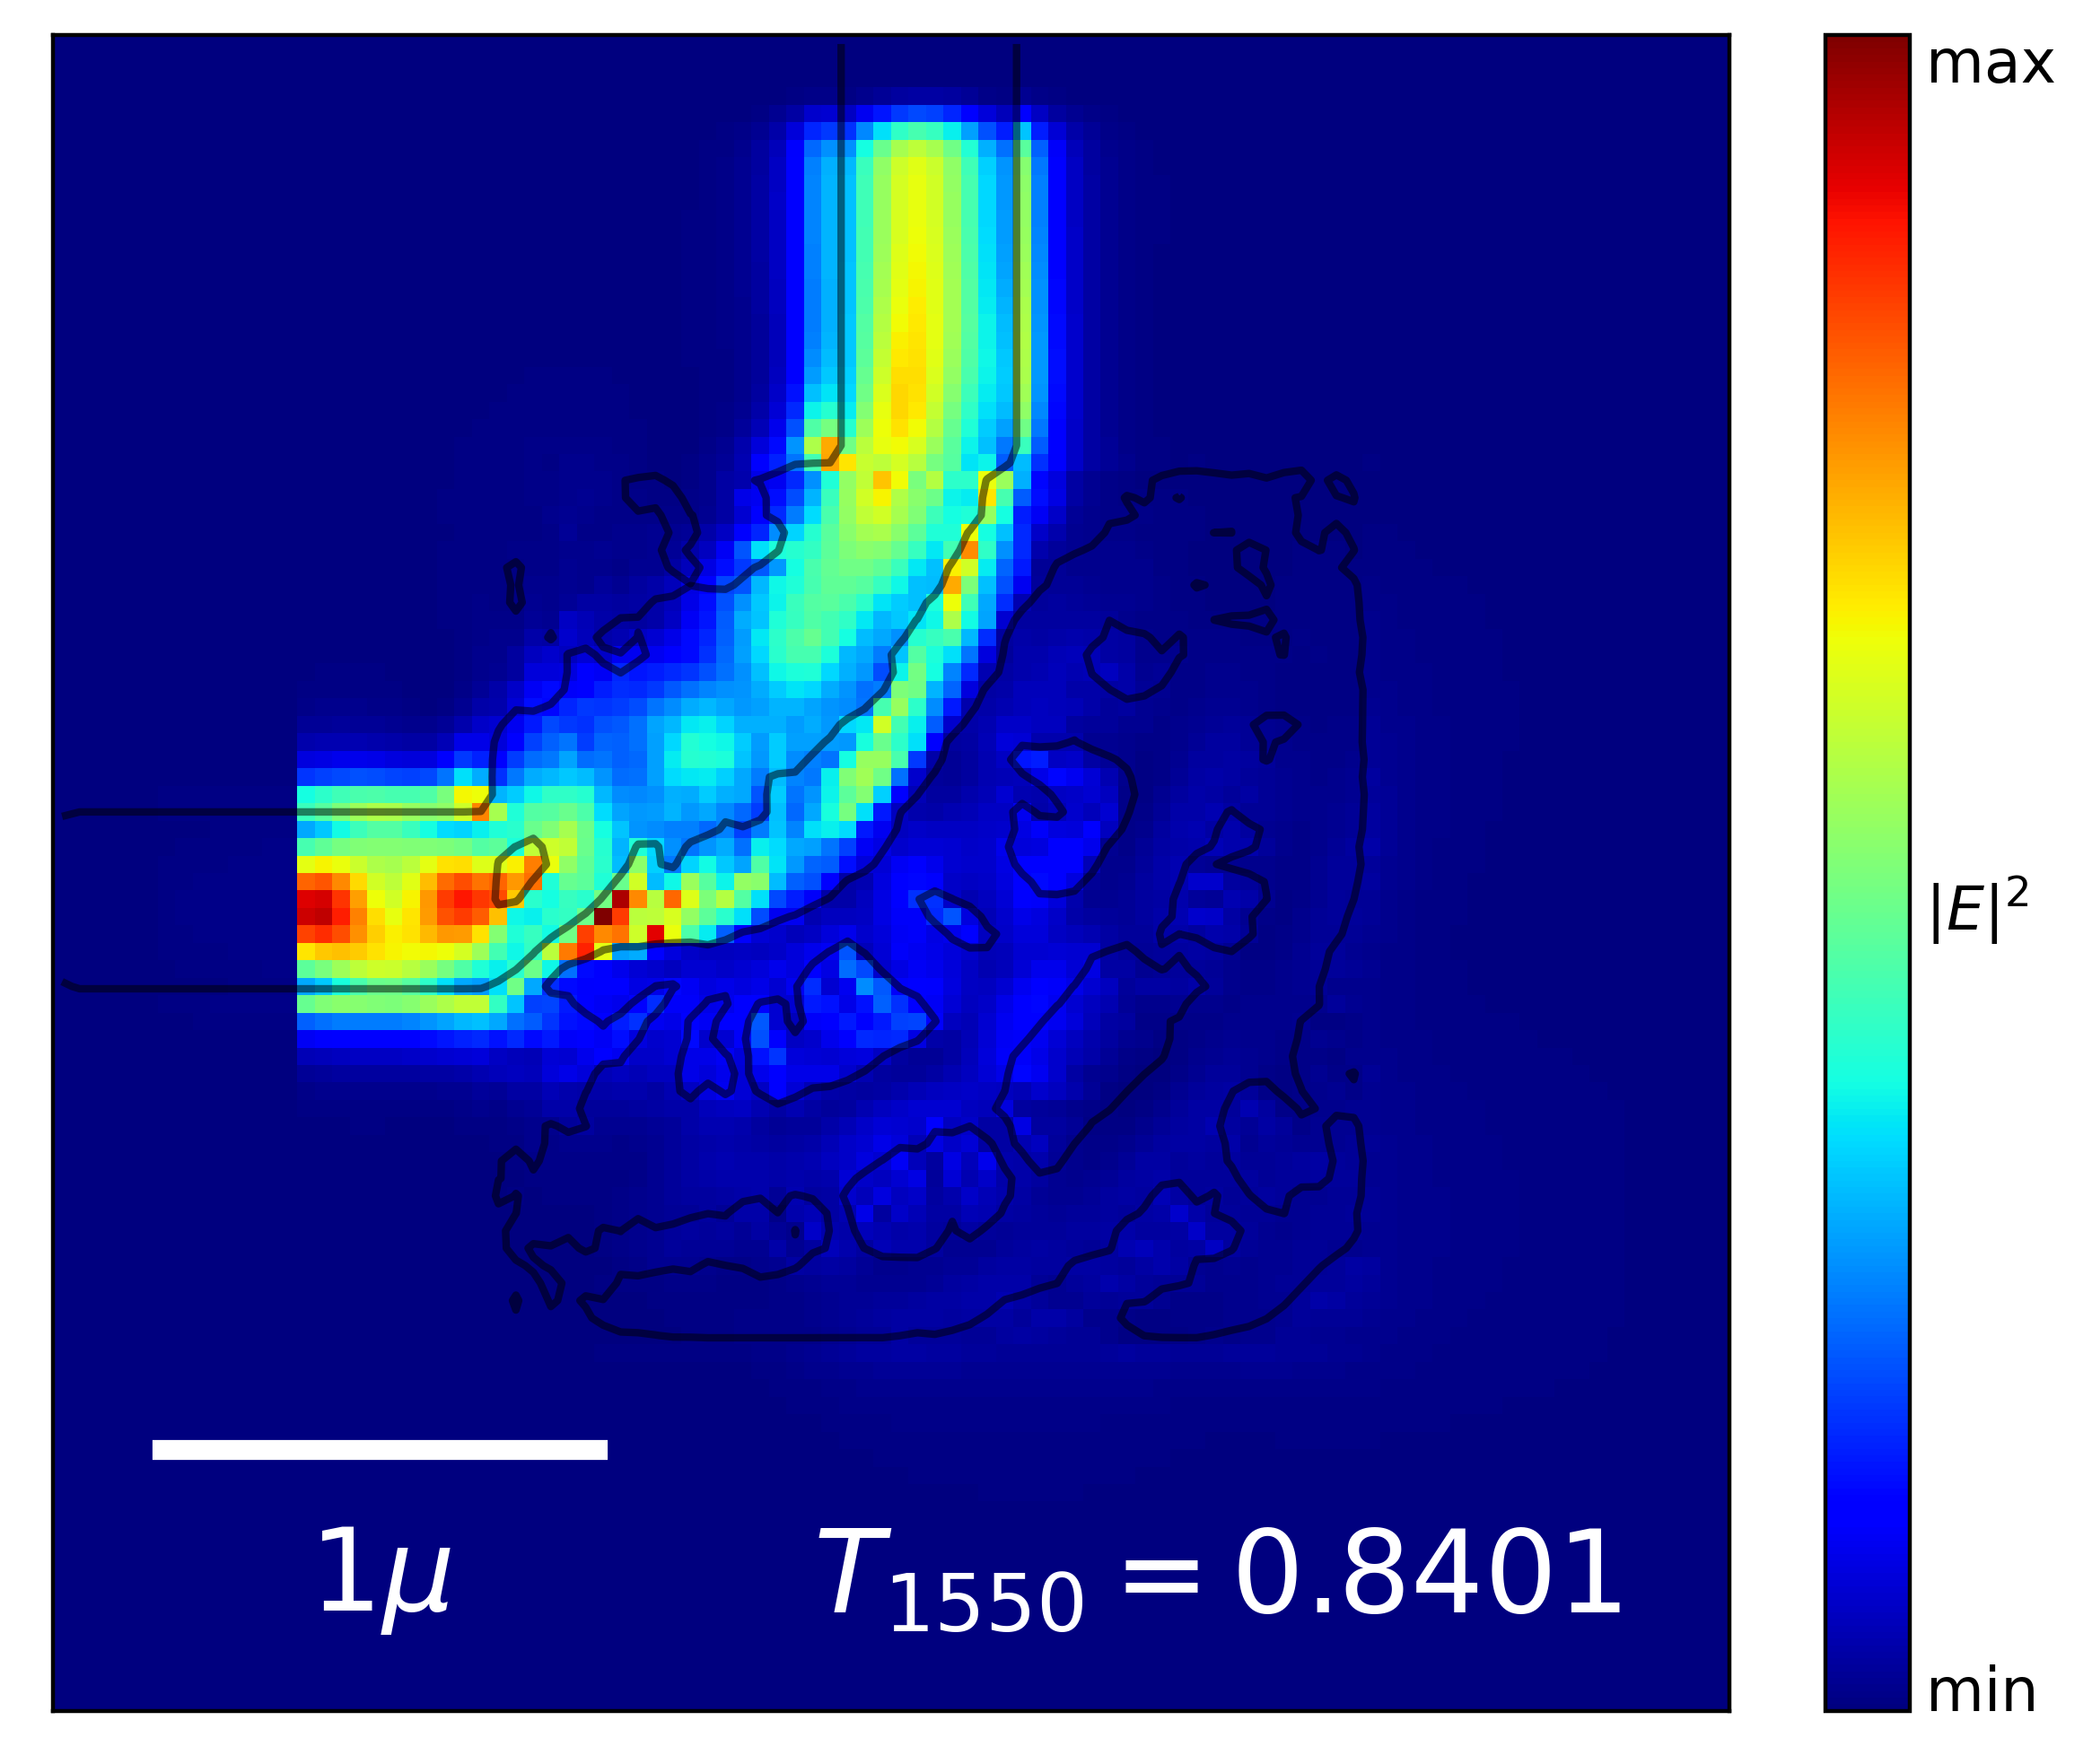
\includegraphics[width=0.33\textwidth]{image/results/bend/CMA-ES/visualize_field_cont_256.png} &
      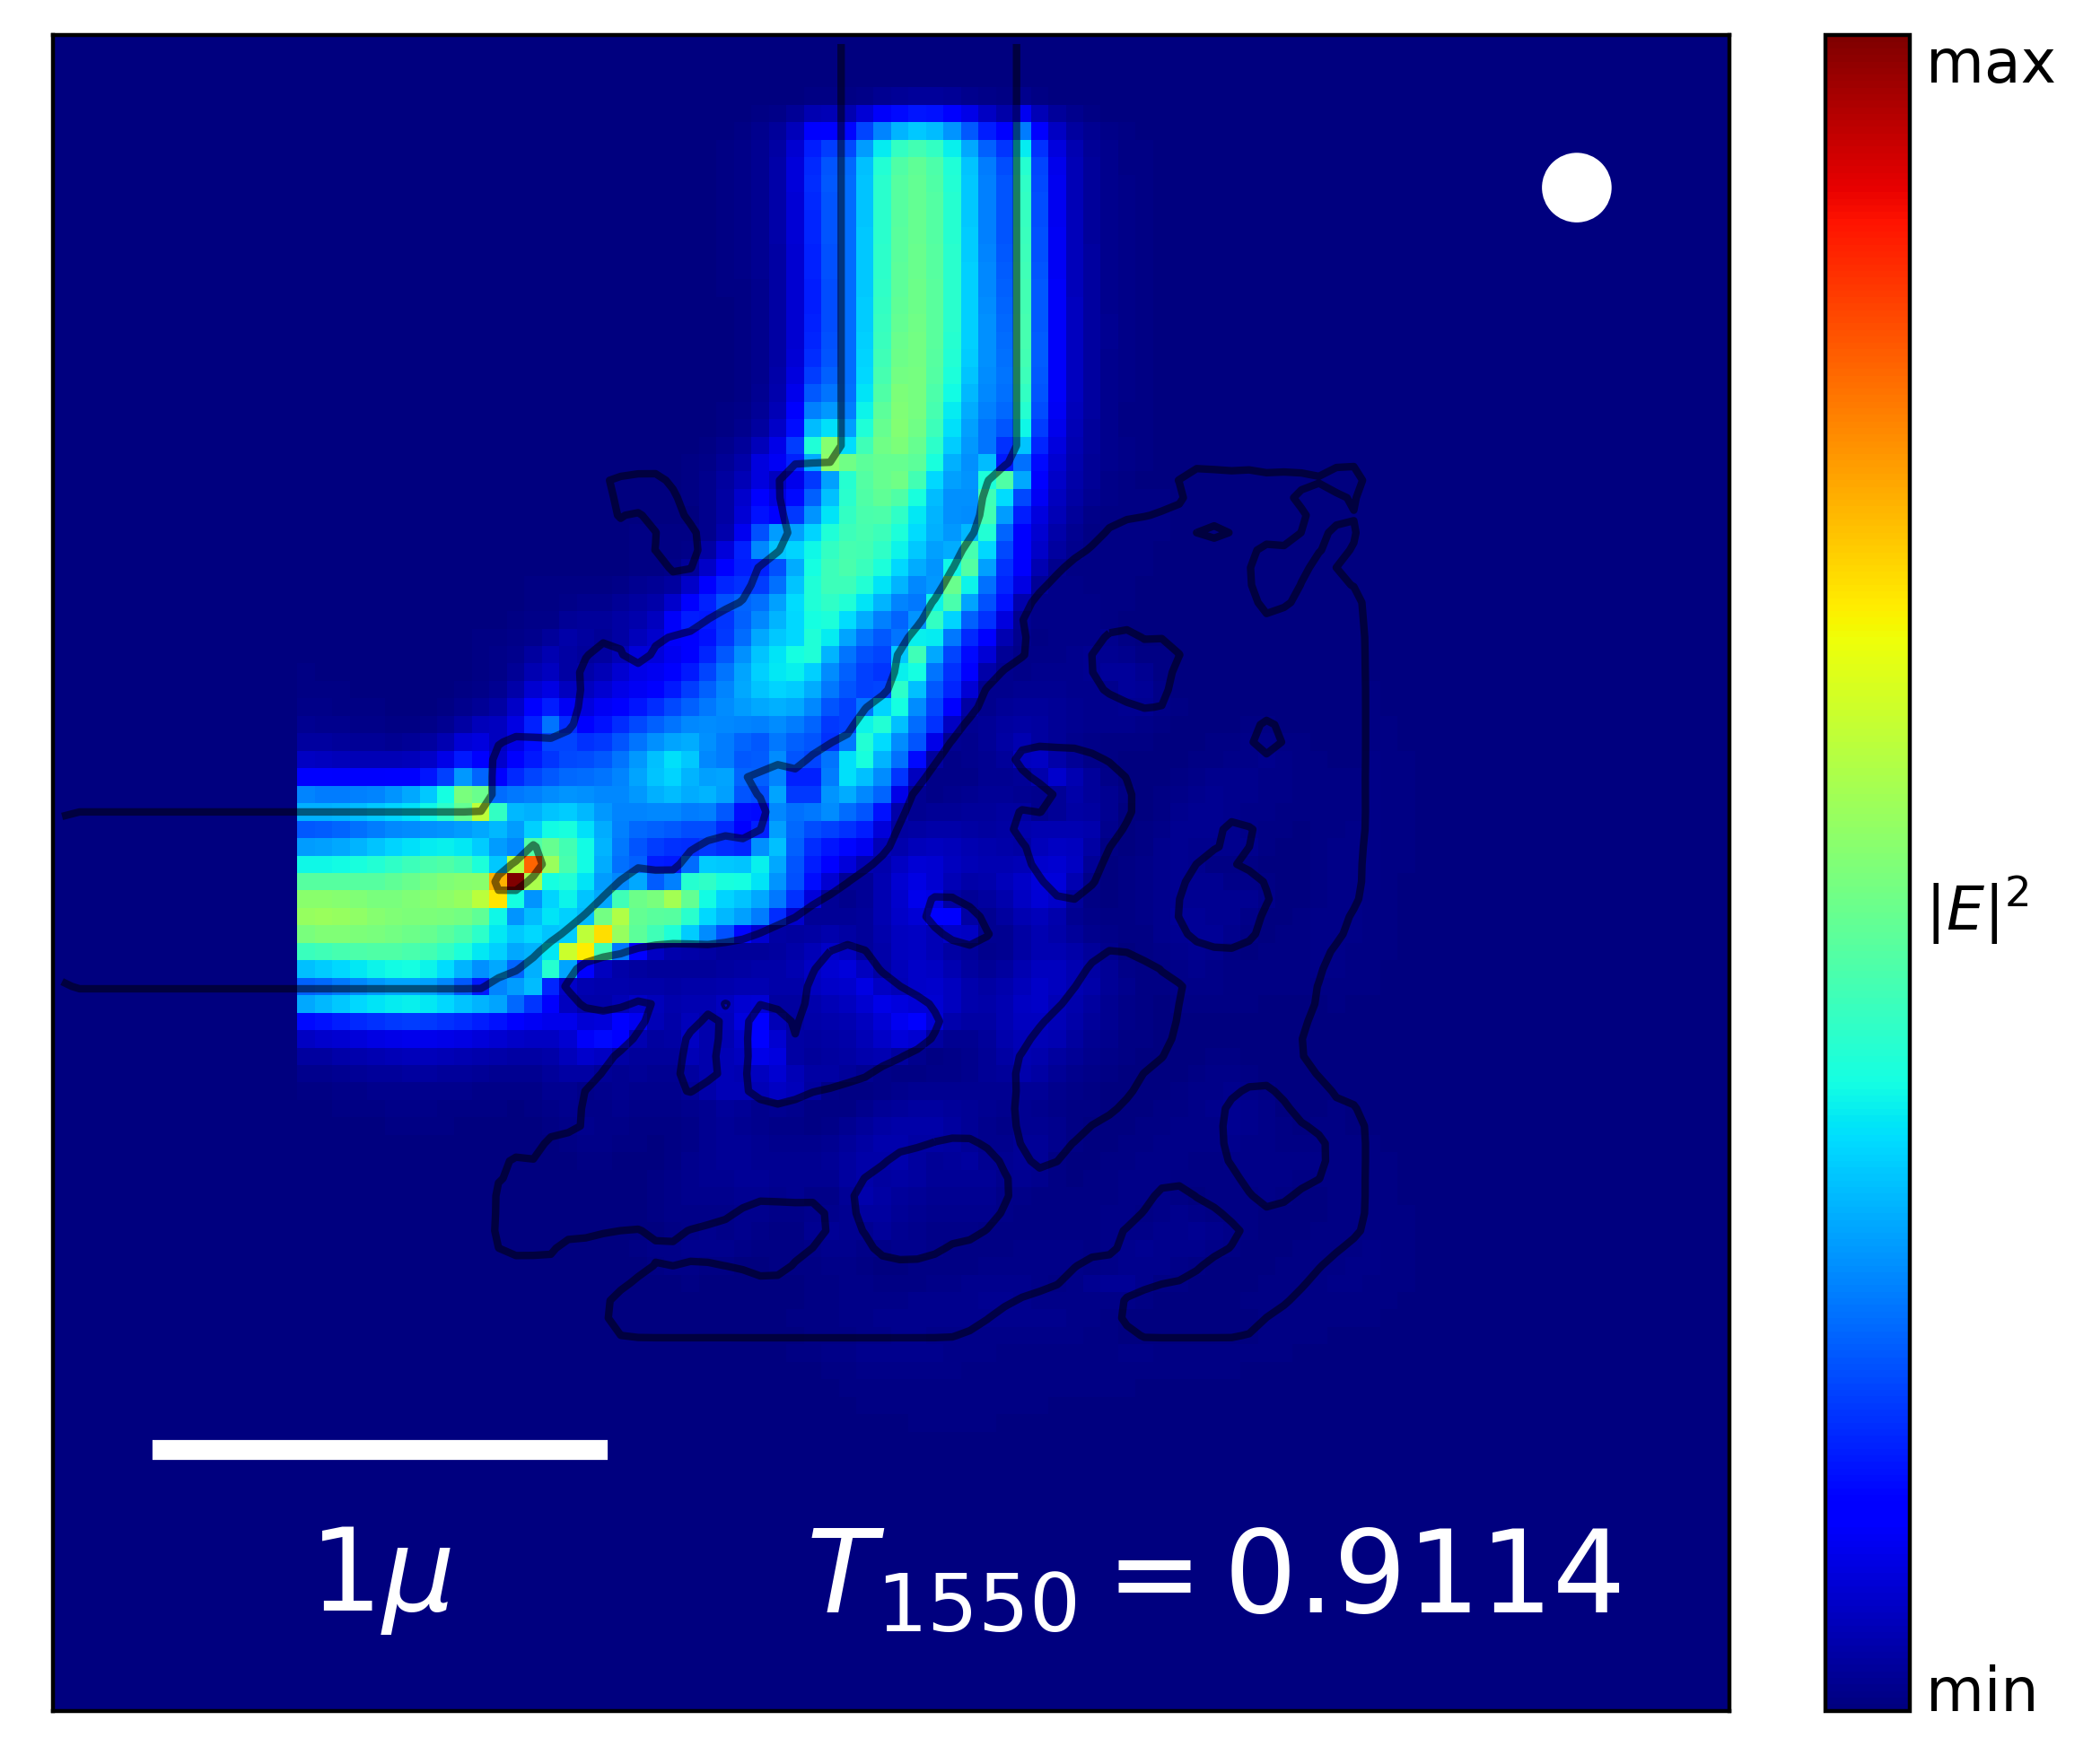
\includegraphics[width=0.33\textwidth]{image/results/bend/CMA-ES/visualize_field_disc_256.png} &
      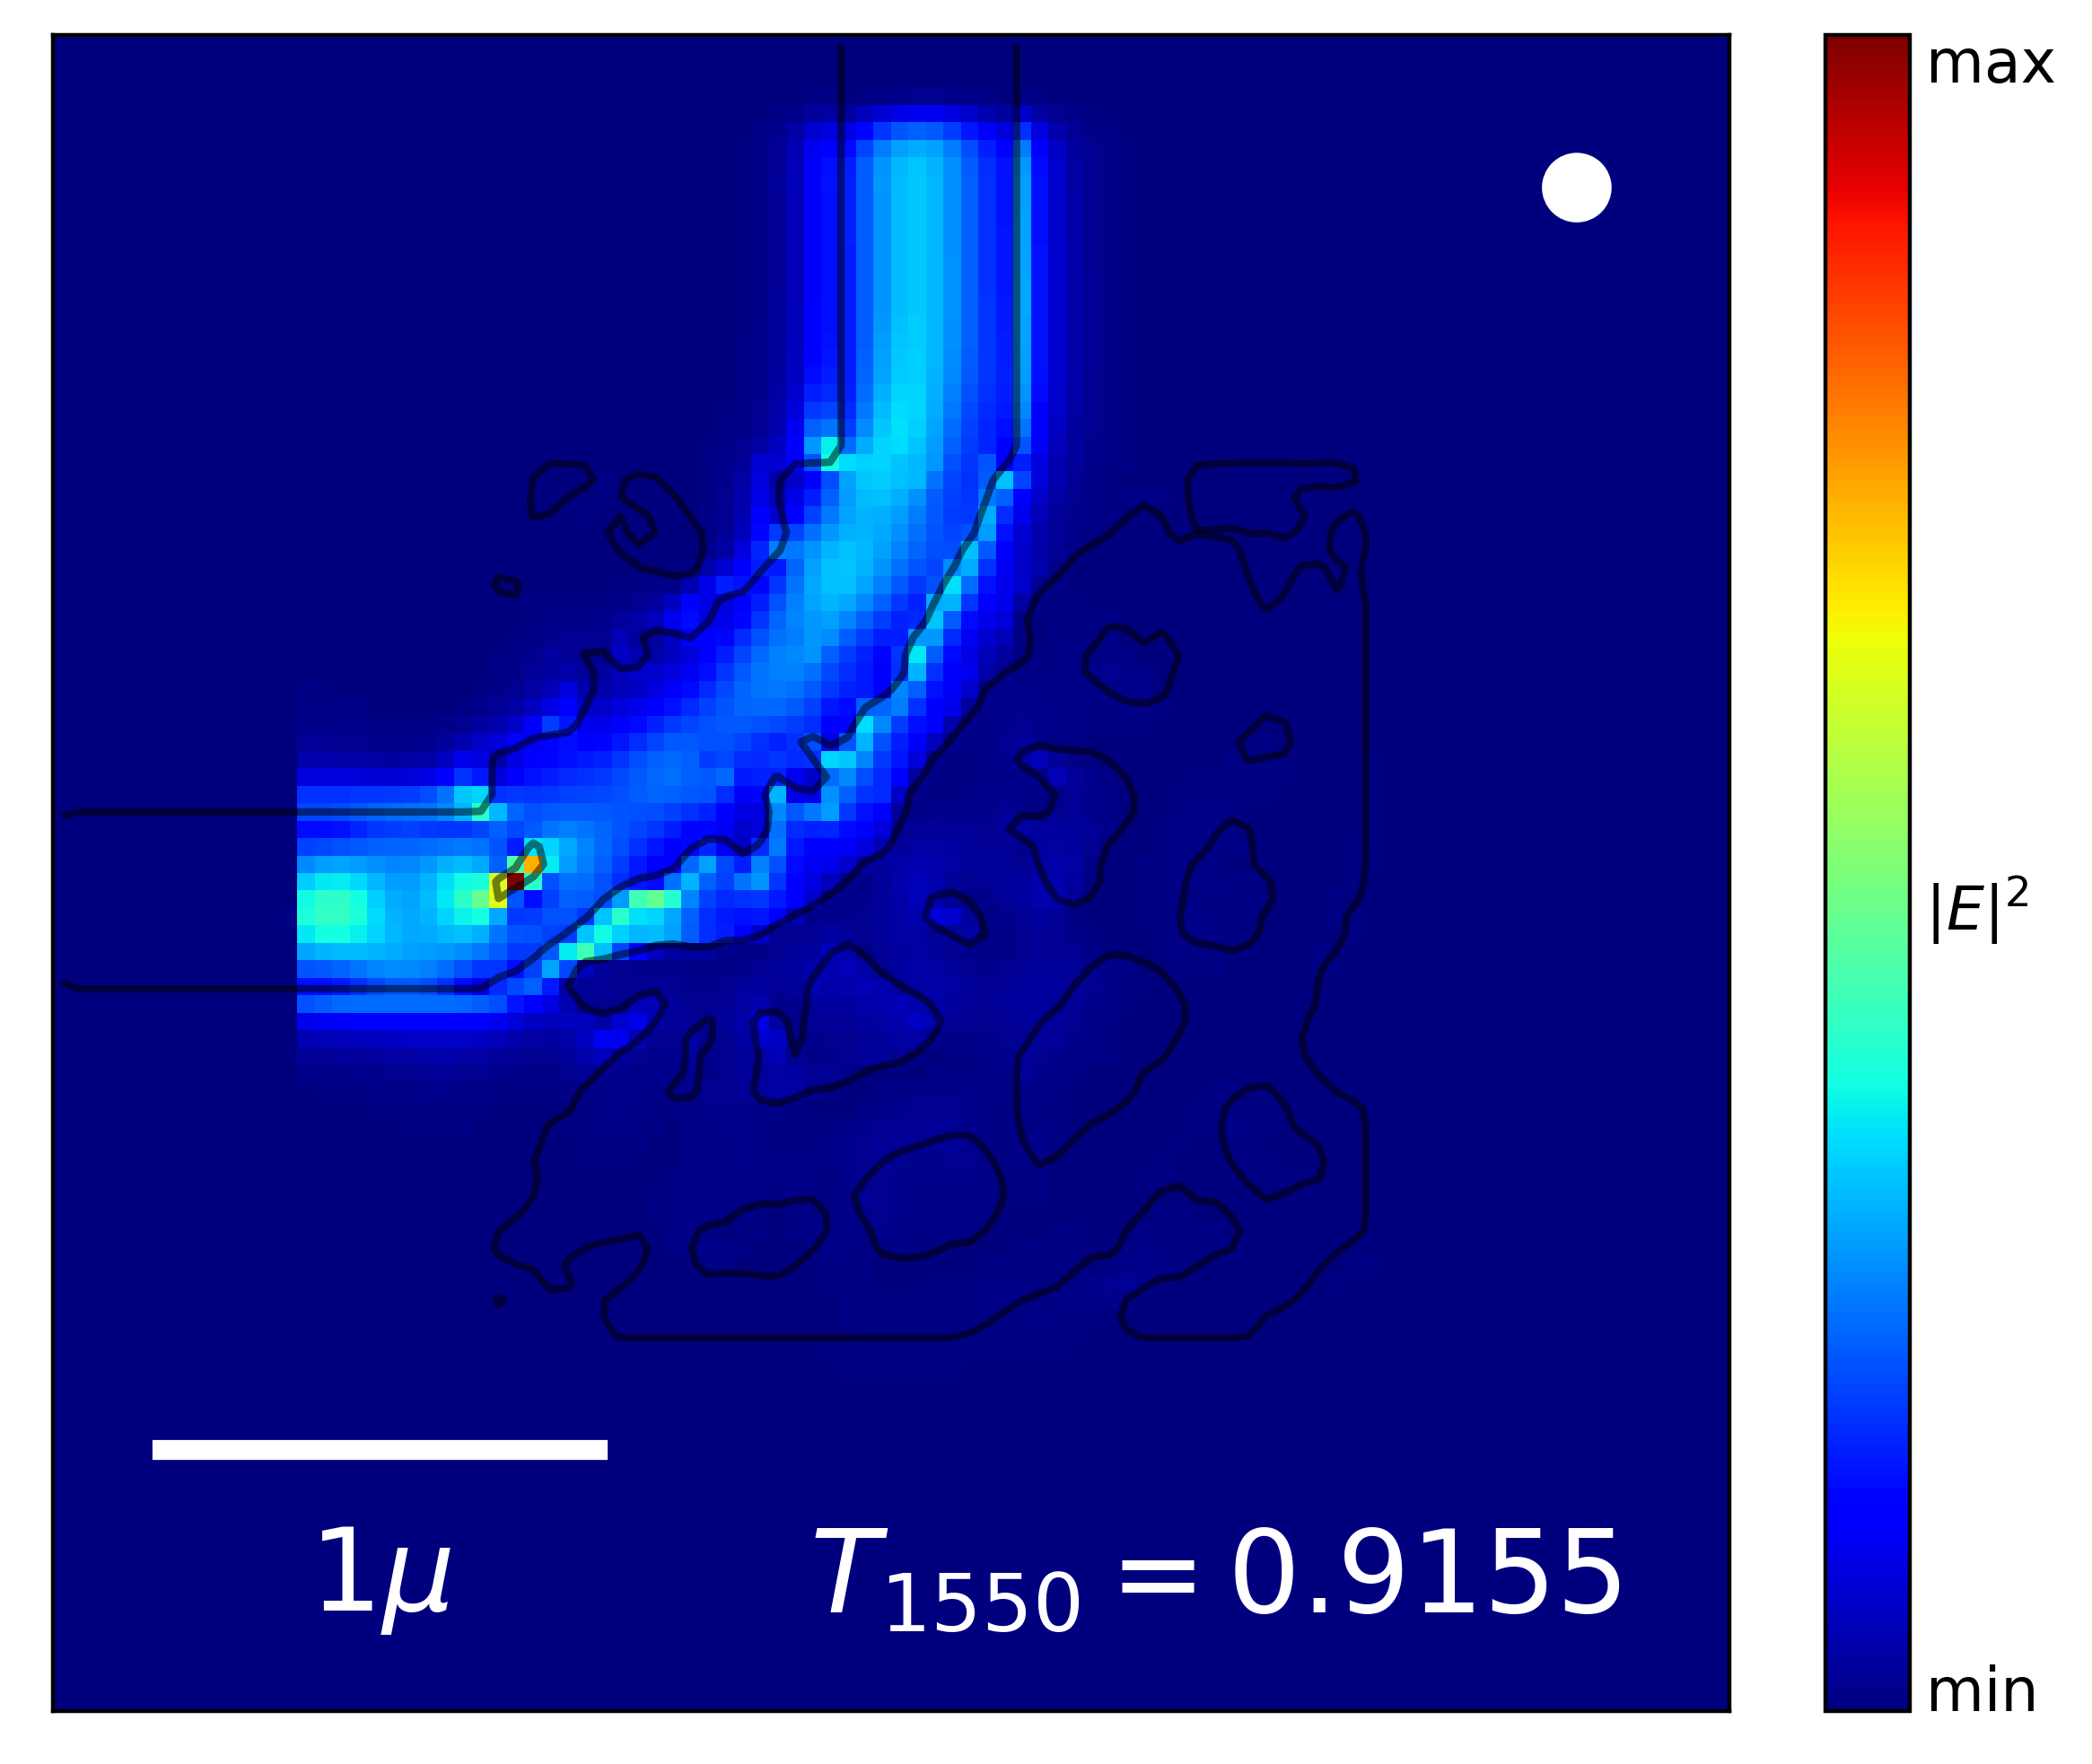
\includegraphics[width=0.33\textwidth]{image/results/bend/CMA-ES/visualize_field_fab_256.png} \\
    \hline
      \multirow{2}{*}{512} &
      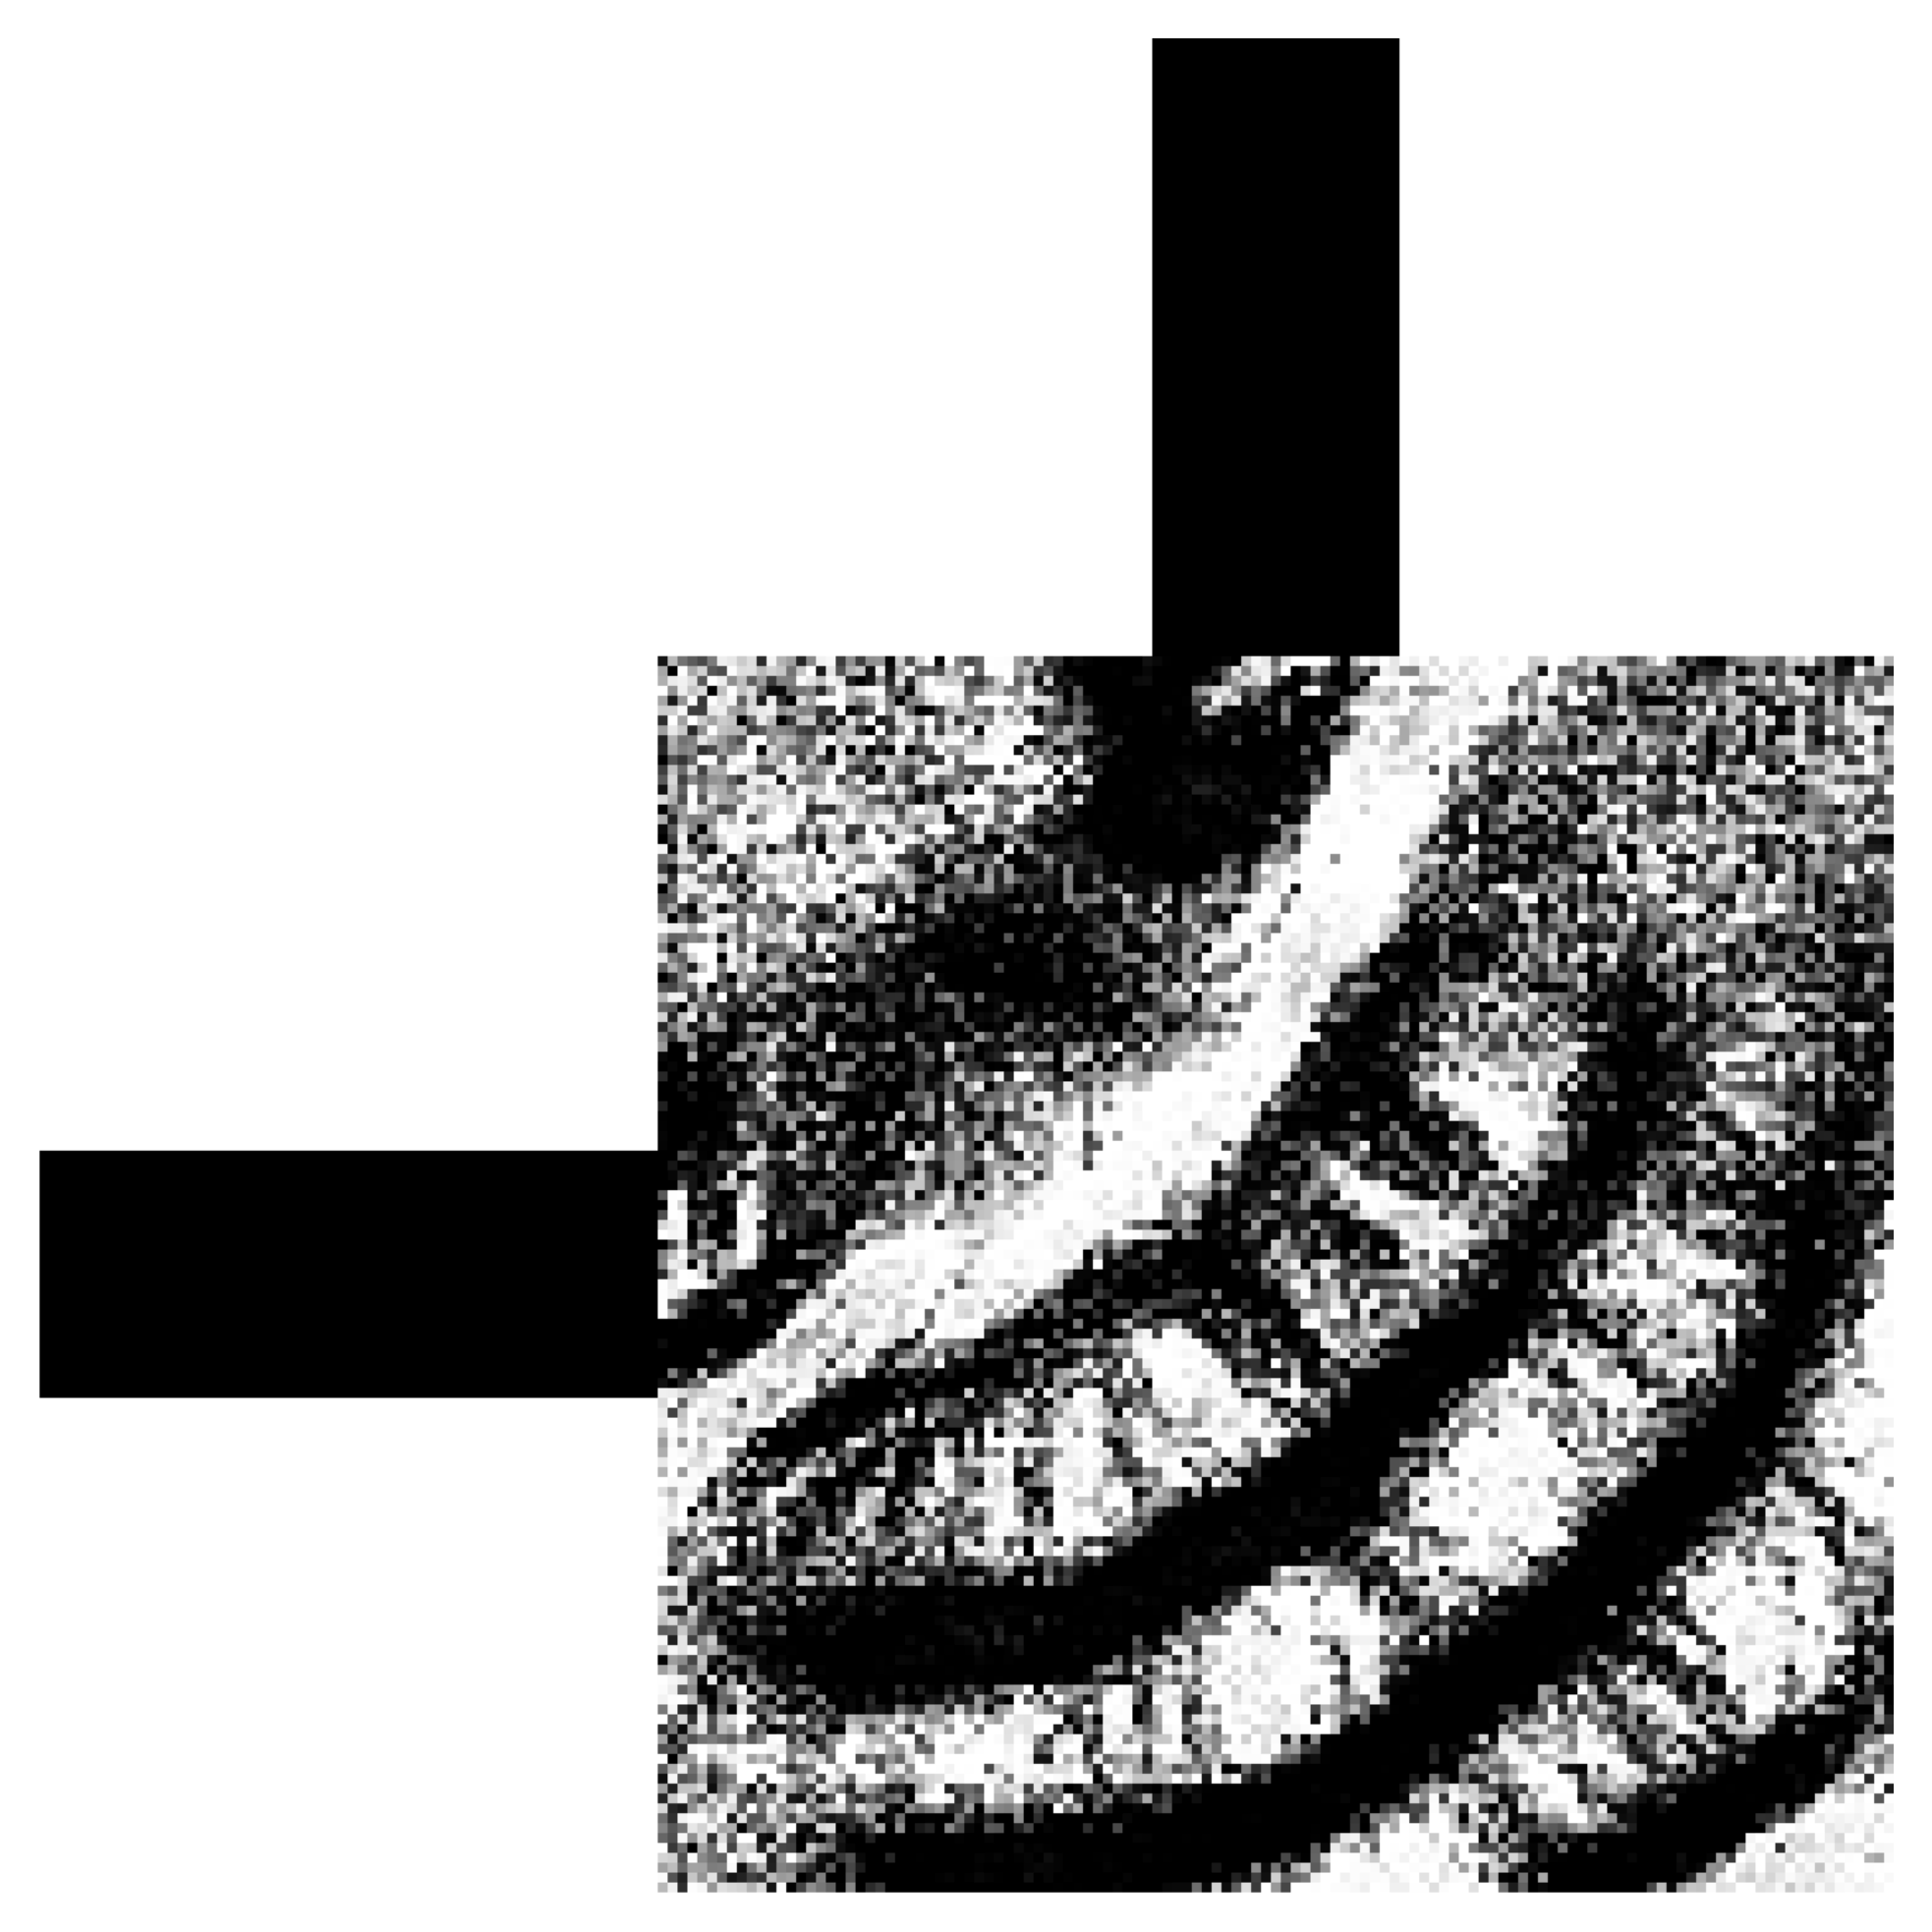
\includegraphics[width=0.20\textwidth]{image/results/bend/CMA-ES/visualize_eps_cont_512.png} &
      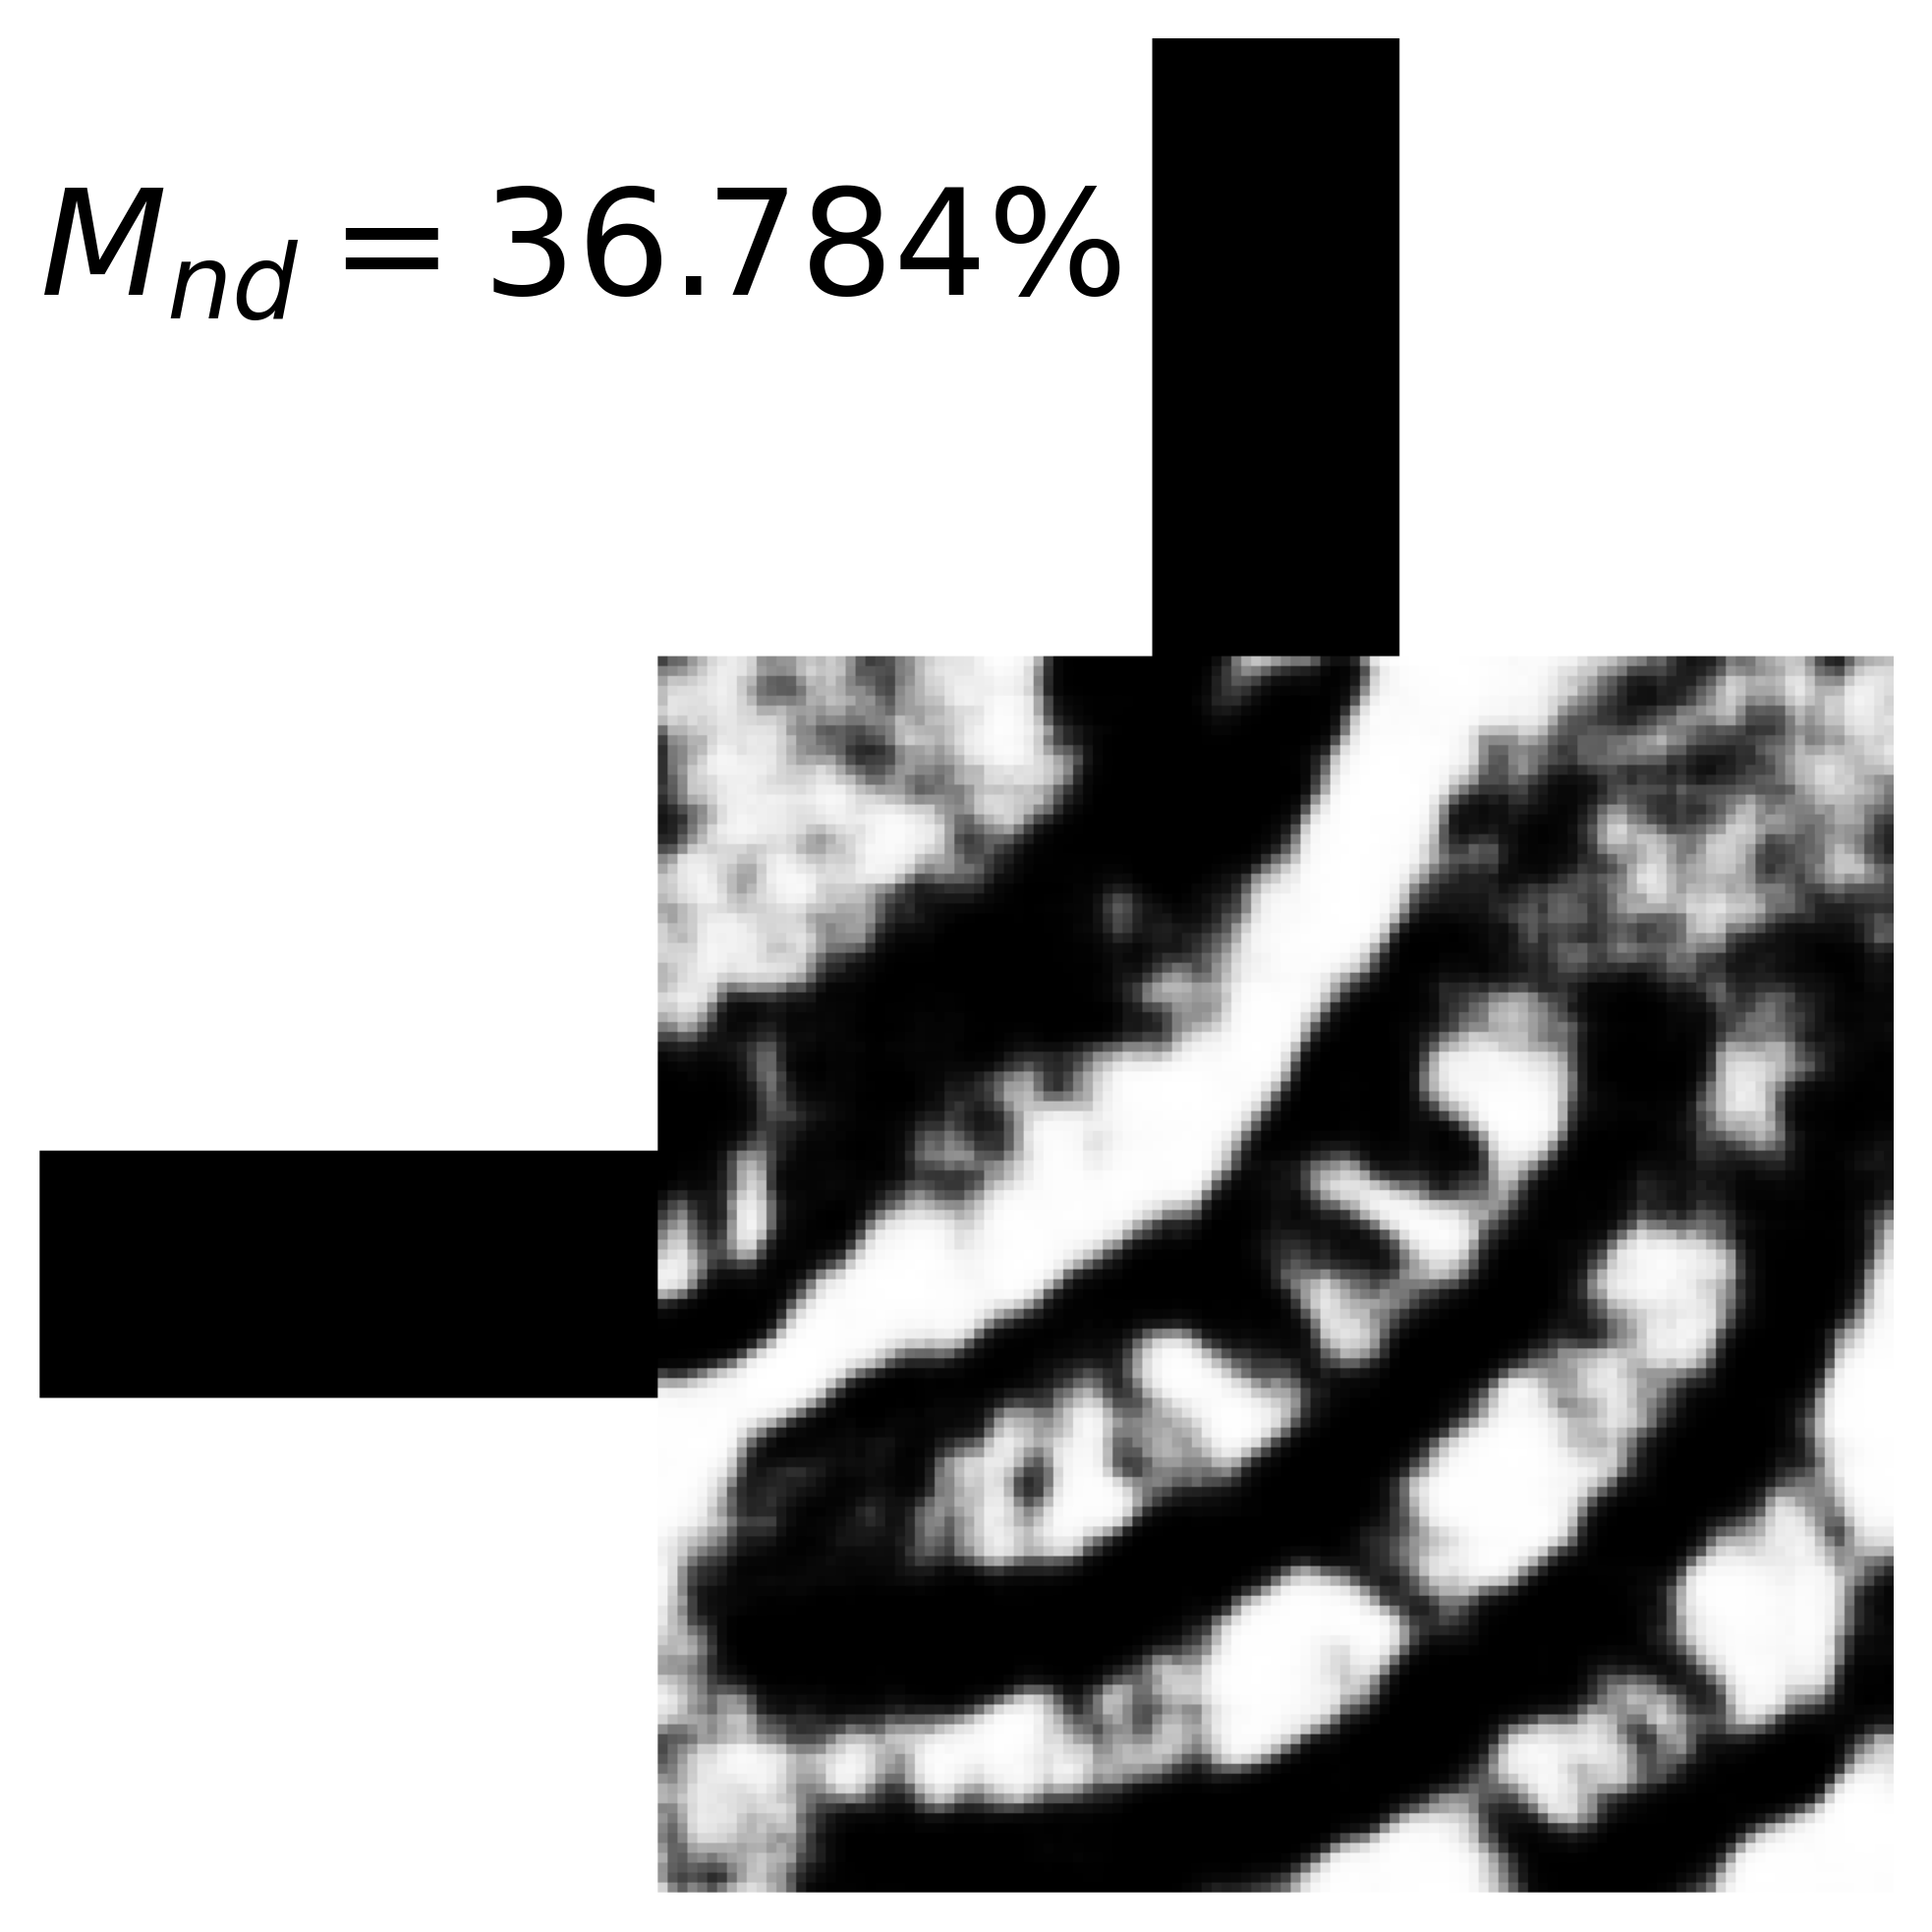
\includegraphics[width=0.20\textwidth]{image/results/bend/CMA-ES/visualize_eps_disc_512.png} &
      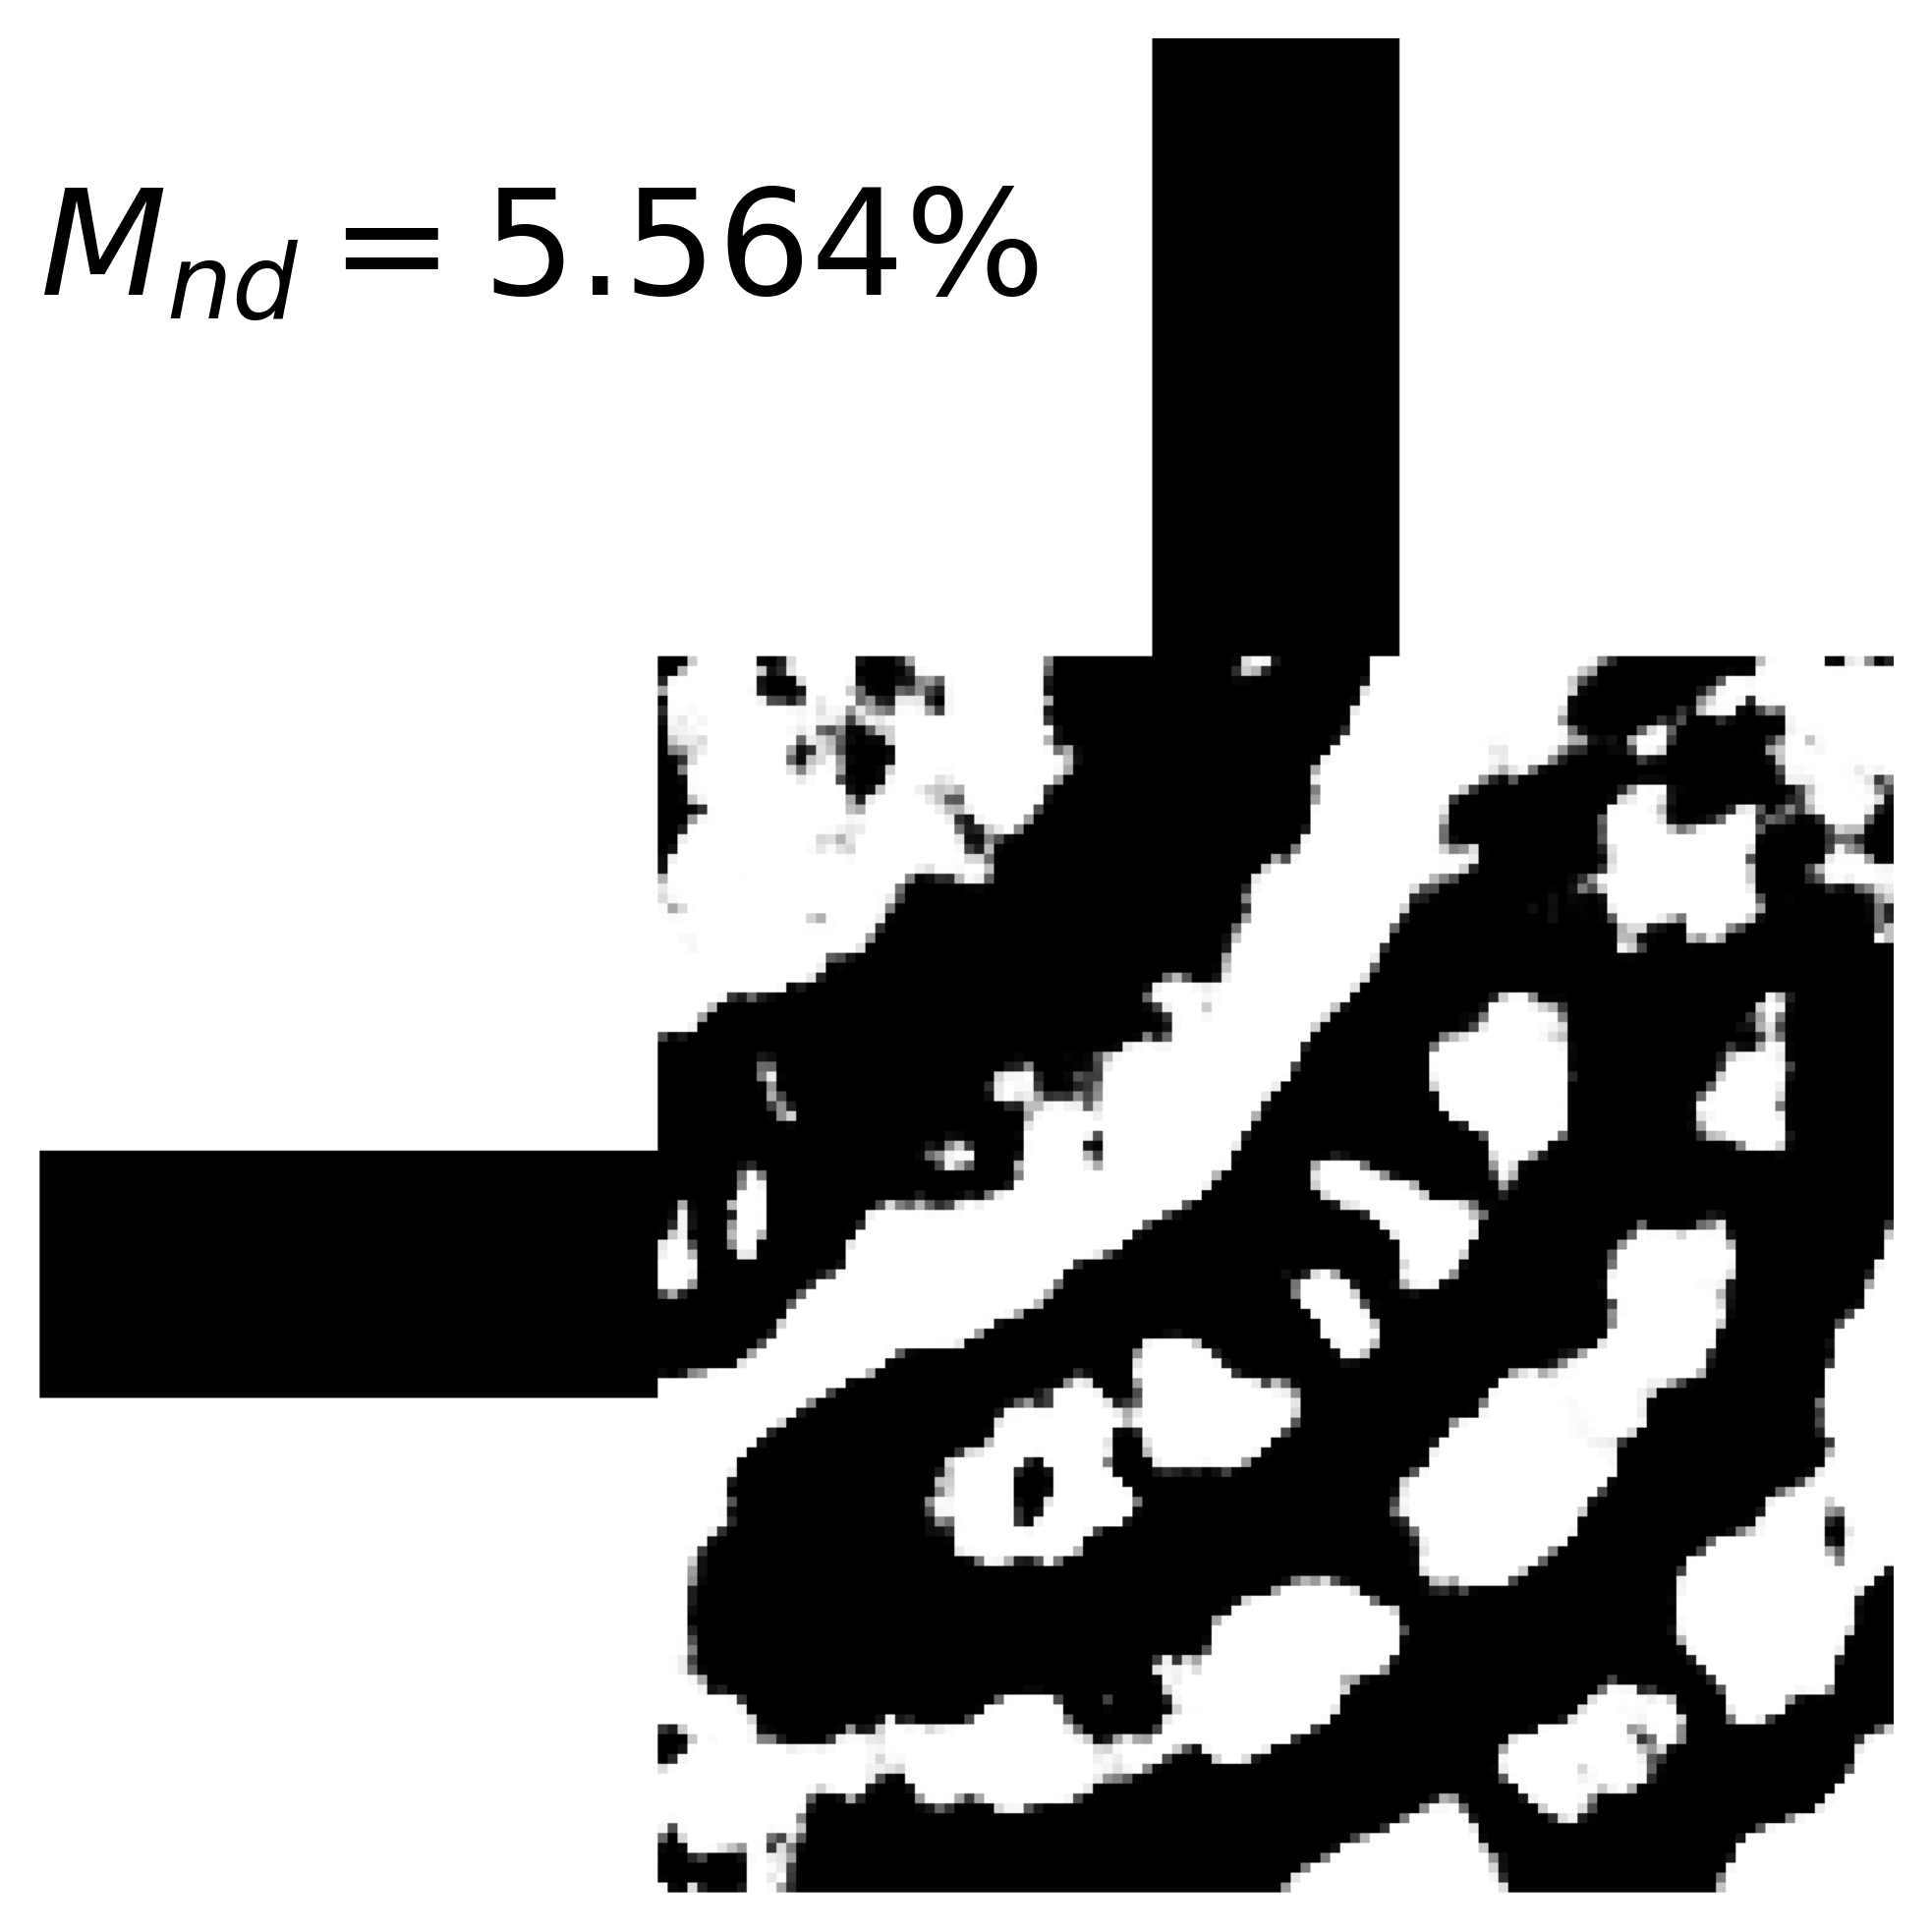
\includegraphics[width=0.20\textwidth]{image/results/bend/CMA-ES/visualize_eps_fab_512.png} \\
      \cline{2-4}
      &
      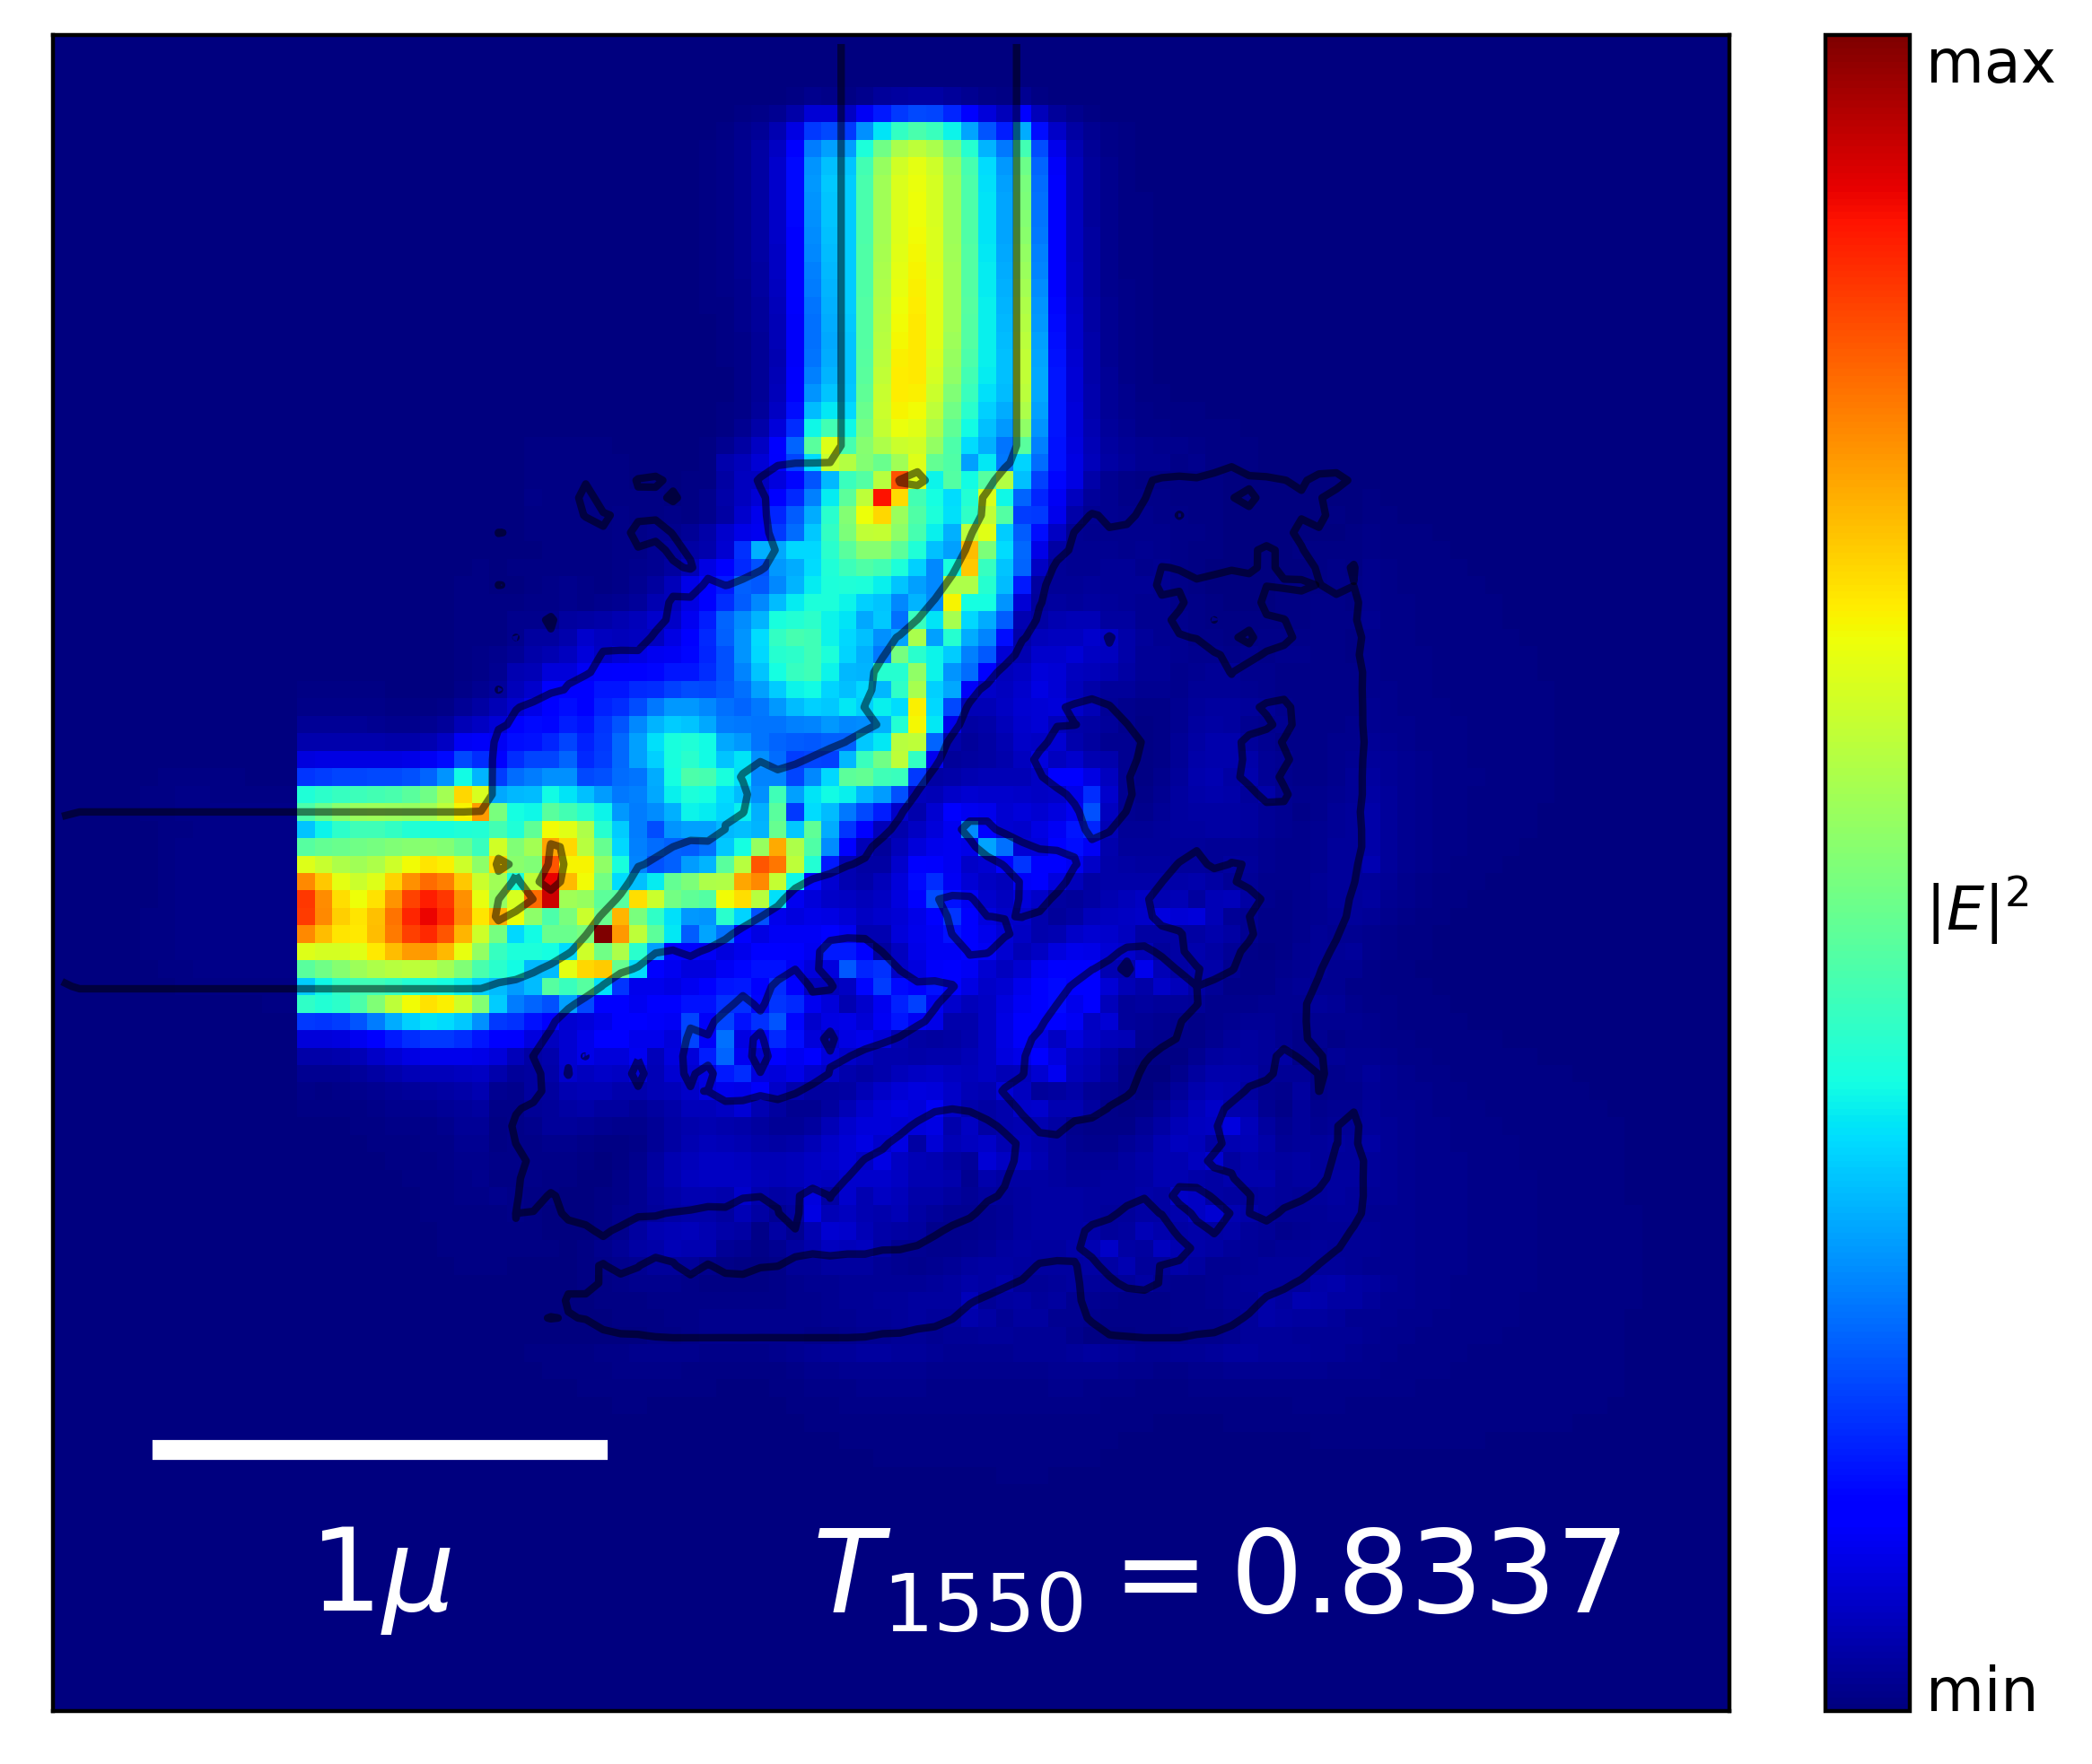
\includegraphics[width=0.33\textwidth]{image/results/bend/CMA-ES/visualize_field_cont_512.png} &
      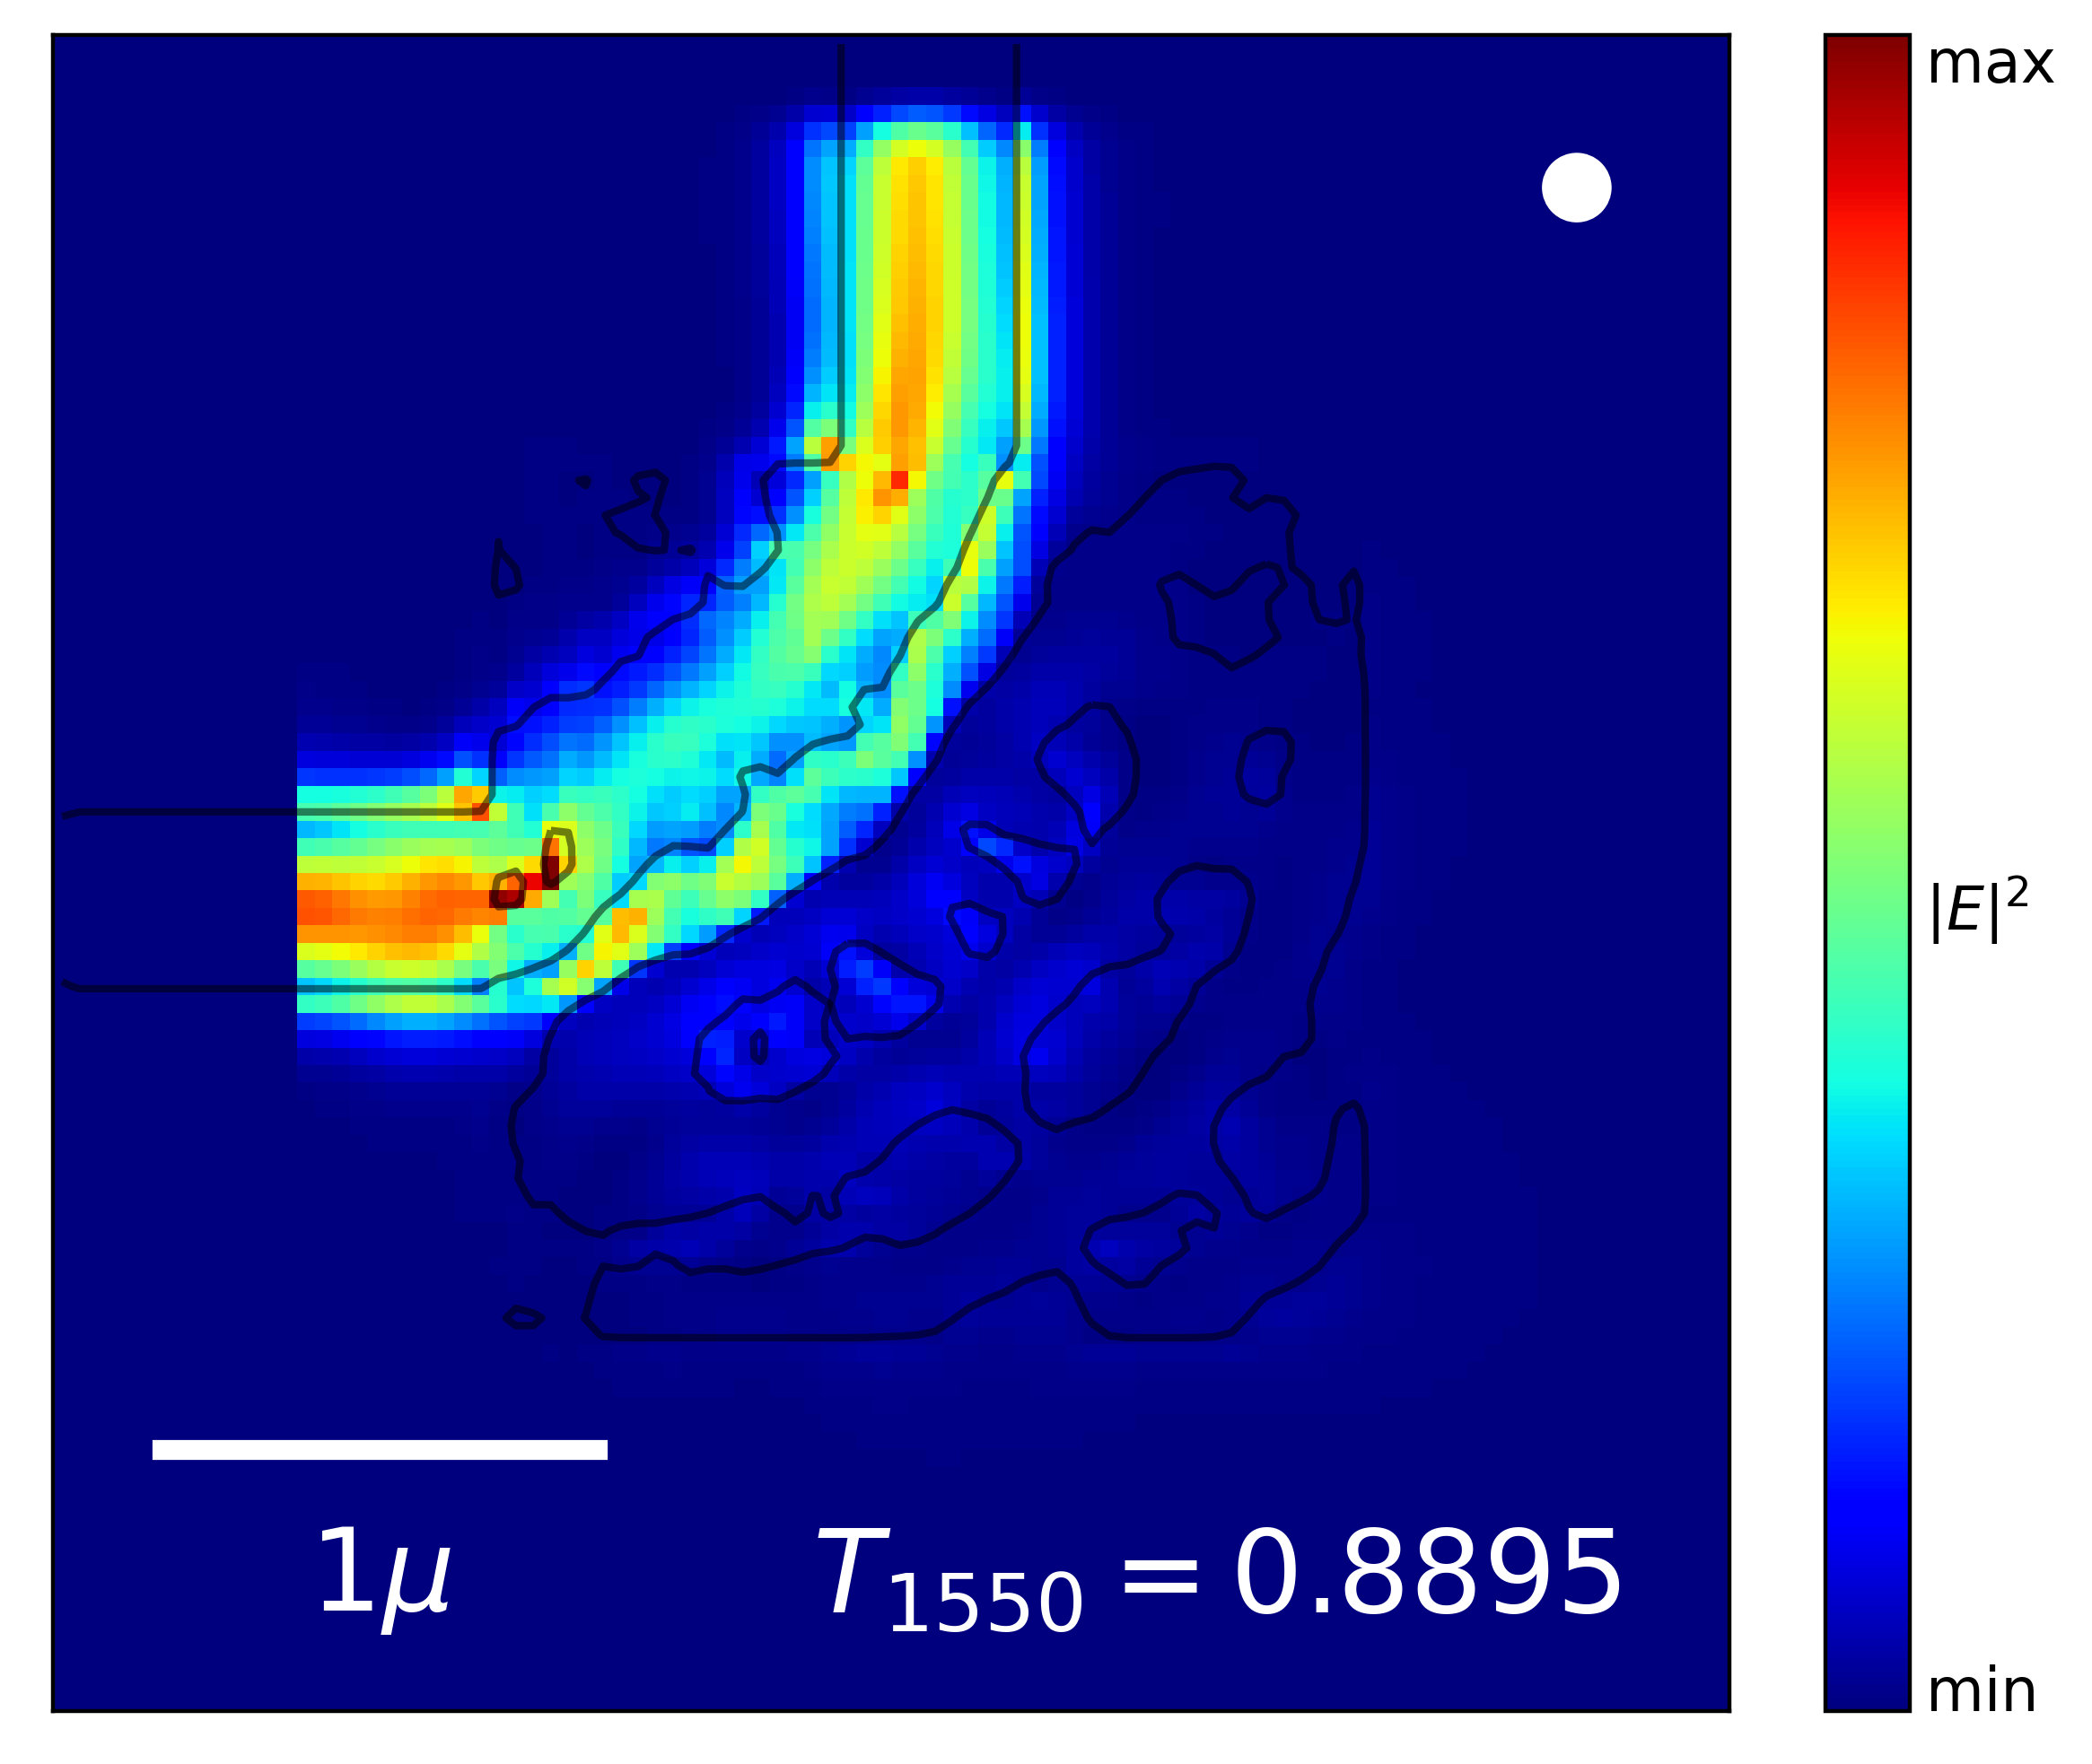
\includegraphics[width=0.33\textwidth]{image/results/bend/CMA-ES/visualize_field_disc_512.png} &
      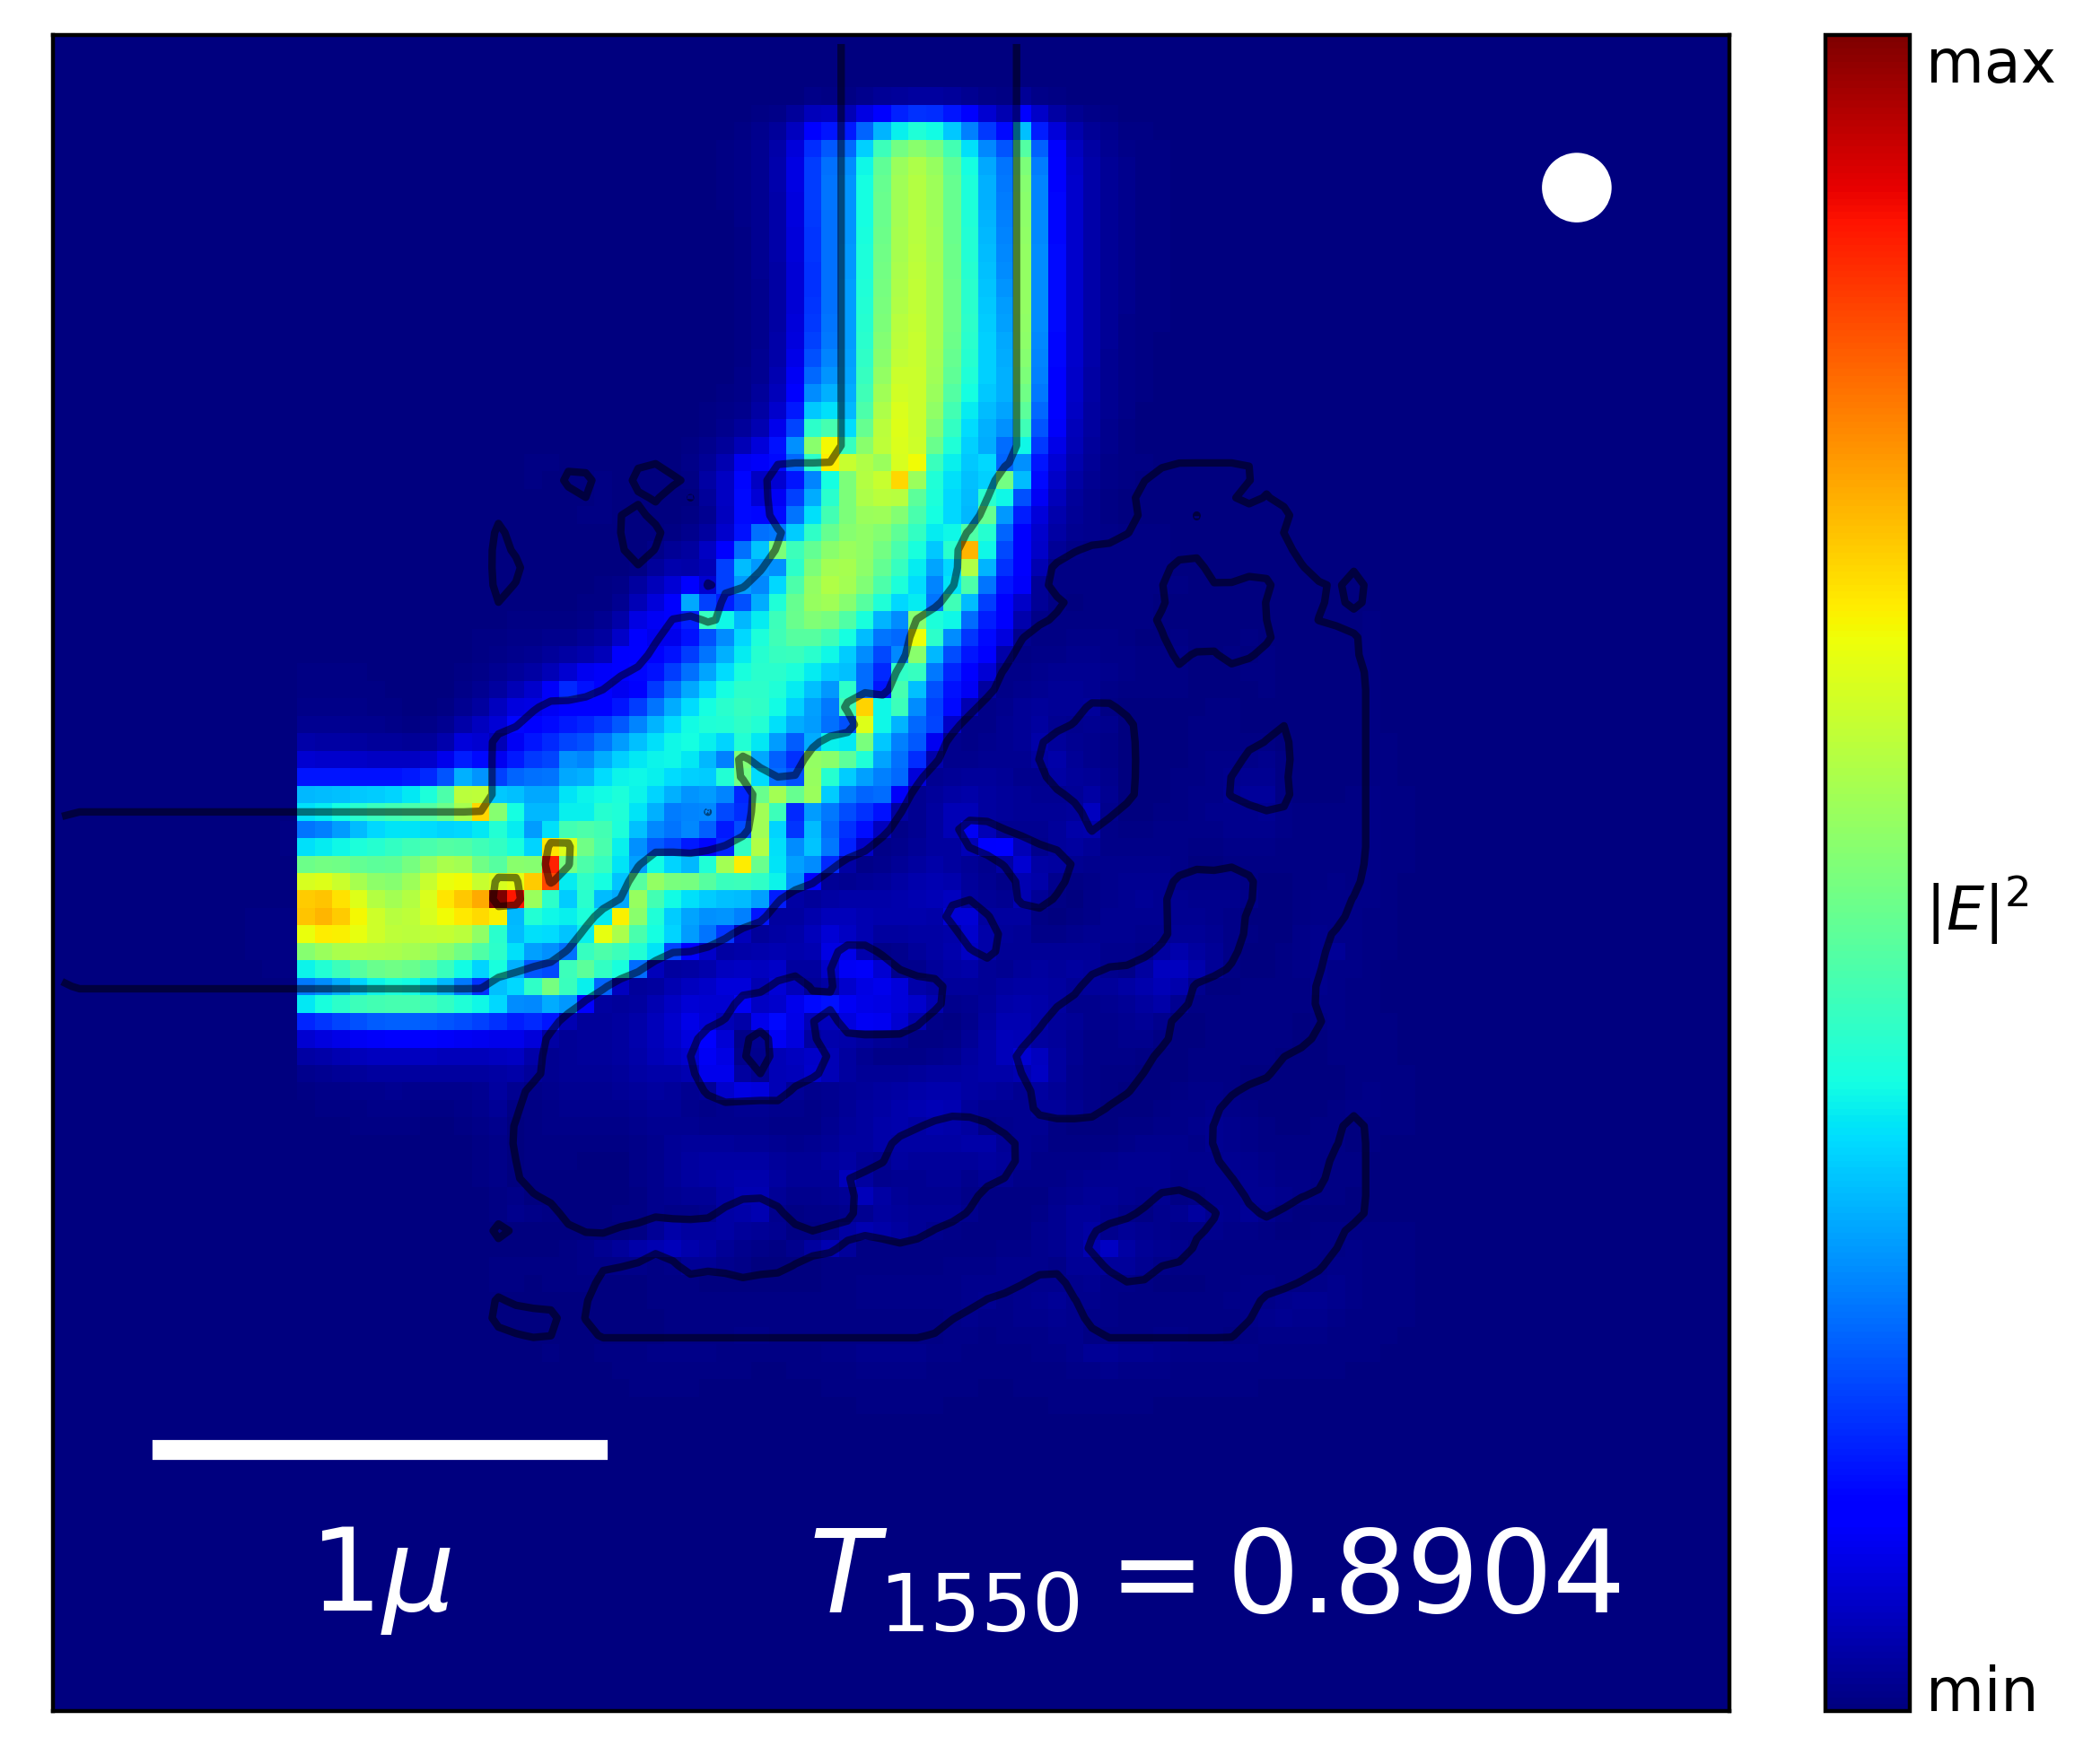
\includegraphics[width=0.33\textwidth]{image/results/bend/CMA-ES/visualize_field_fab_512.png} \\
    \hline
    \end{tabular}
    \hspace*{-3cm}
    \caption{Resultados de optimizar el \emph{bend} usando G-CMA-ES.}
    \label{tab:opt-CMA-bend}
\end{table}


% Bend - MMA
\begin{table}[ht]
    \centering
    \vspace*{-2.5cm}
    \hspace*{-3cm}
    \begin{tabular}{|c|c|c|c|}
    \hline 
    \emph{Seed} & Opt. continua & Opt. discreta &  Opt. de fabricación \\
    \hline
      \multirow{2}{*}{128} &
      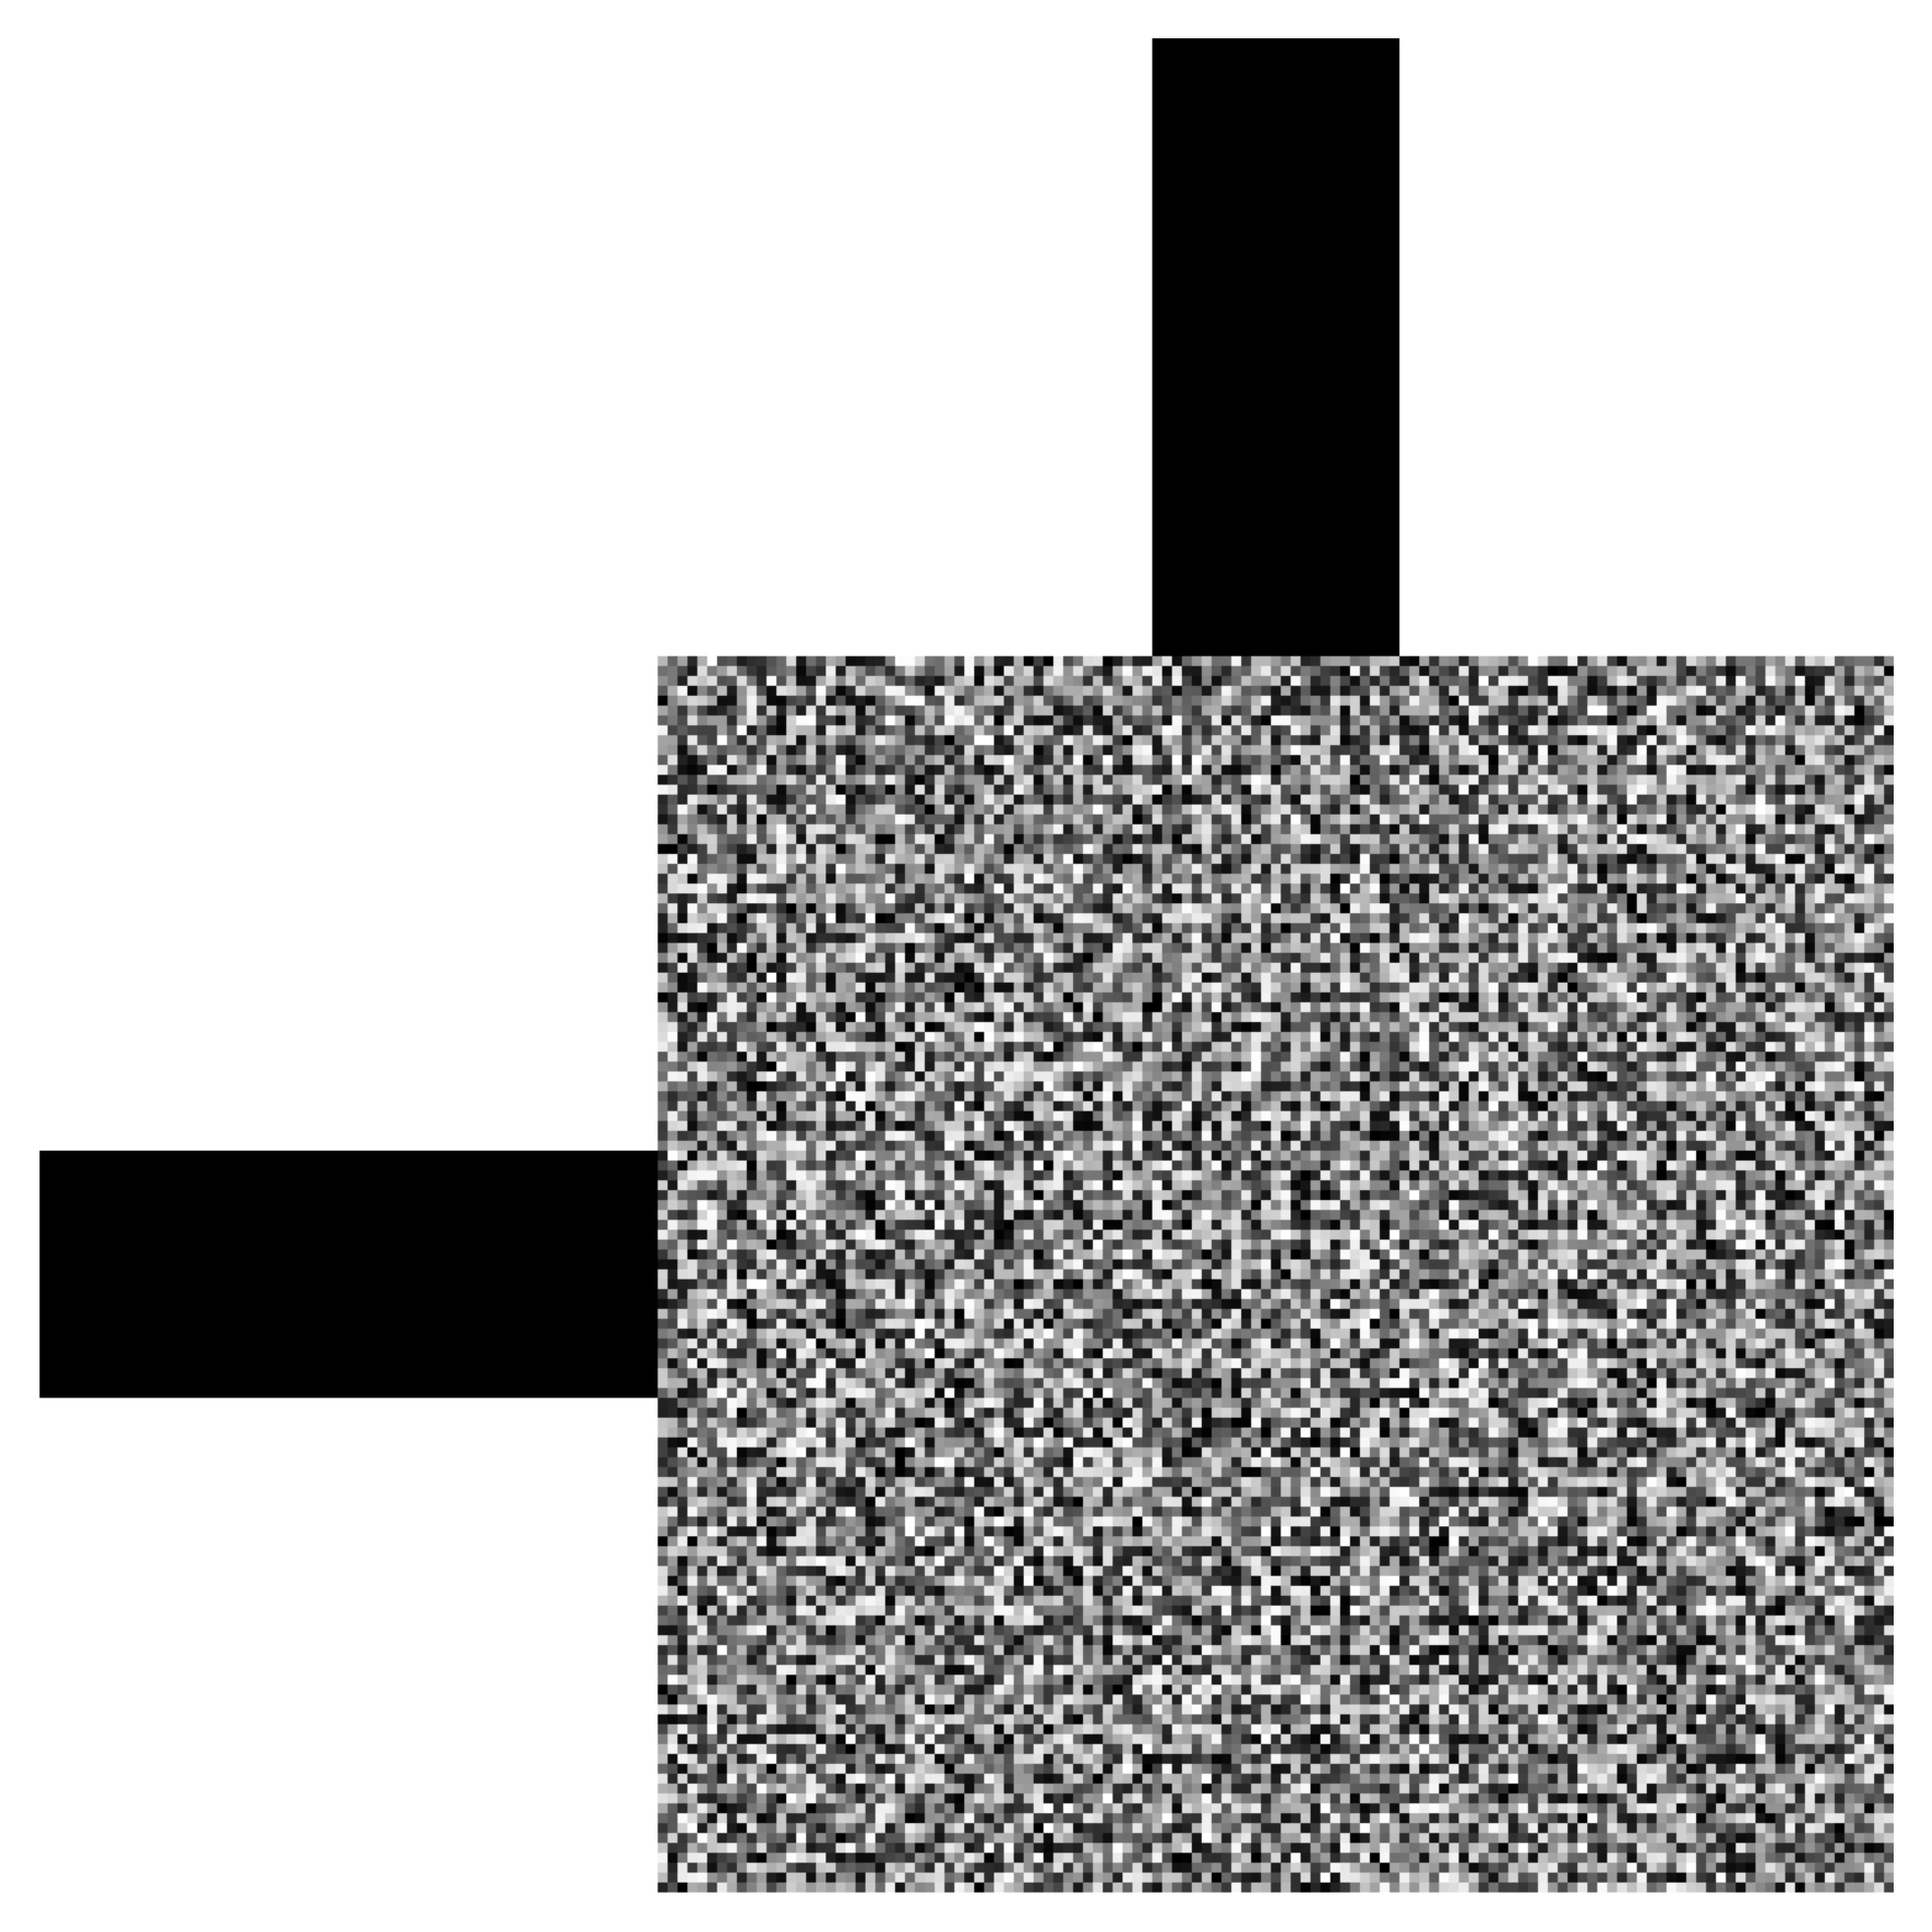
\includegraphics[width=0.20\textwidth]{image/results/bend/MMA/visualize_eps_cont_128.png} &
      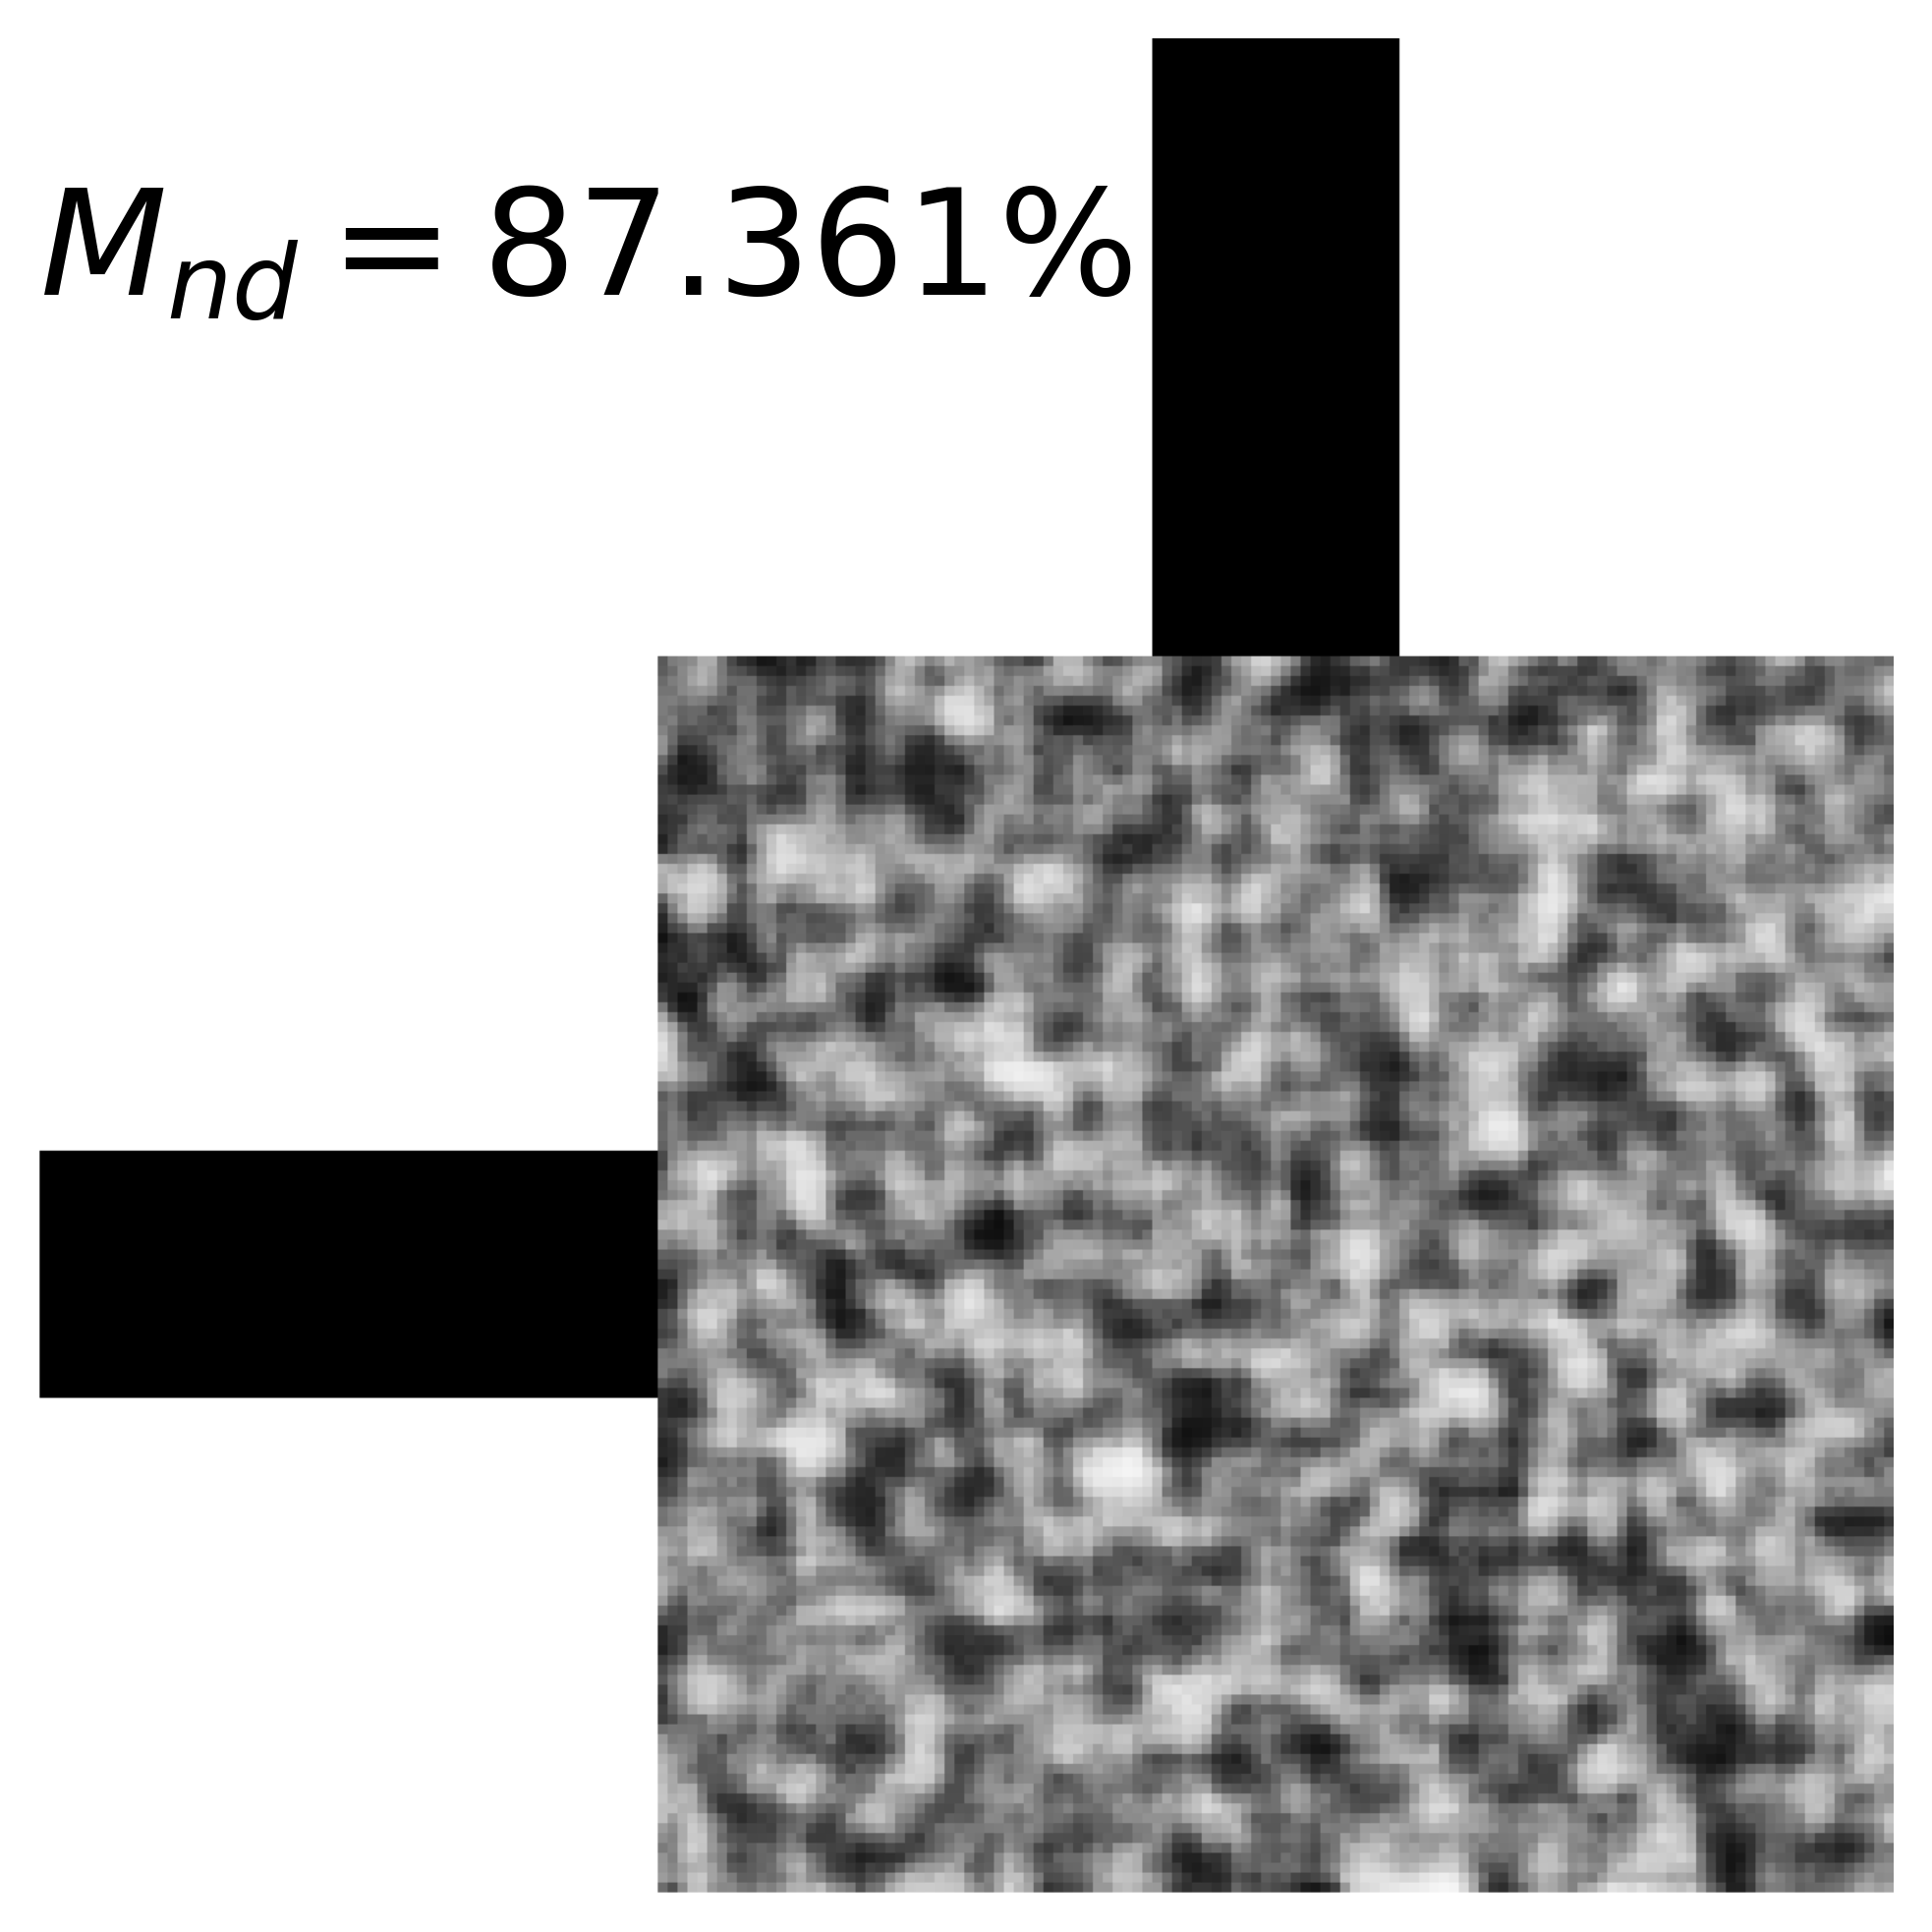
\includegraphics[width=0.20\textwidth]{image/results/bend/MMA/visualize_eps_disc_128.png} &
      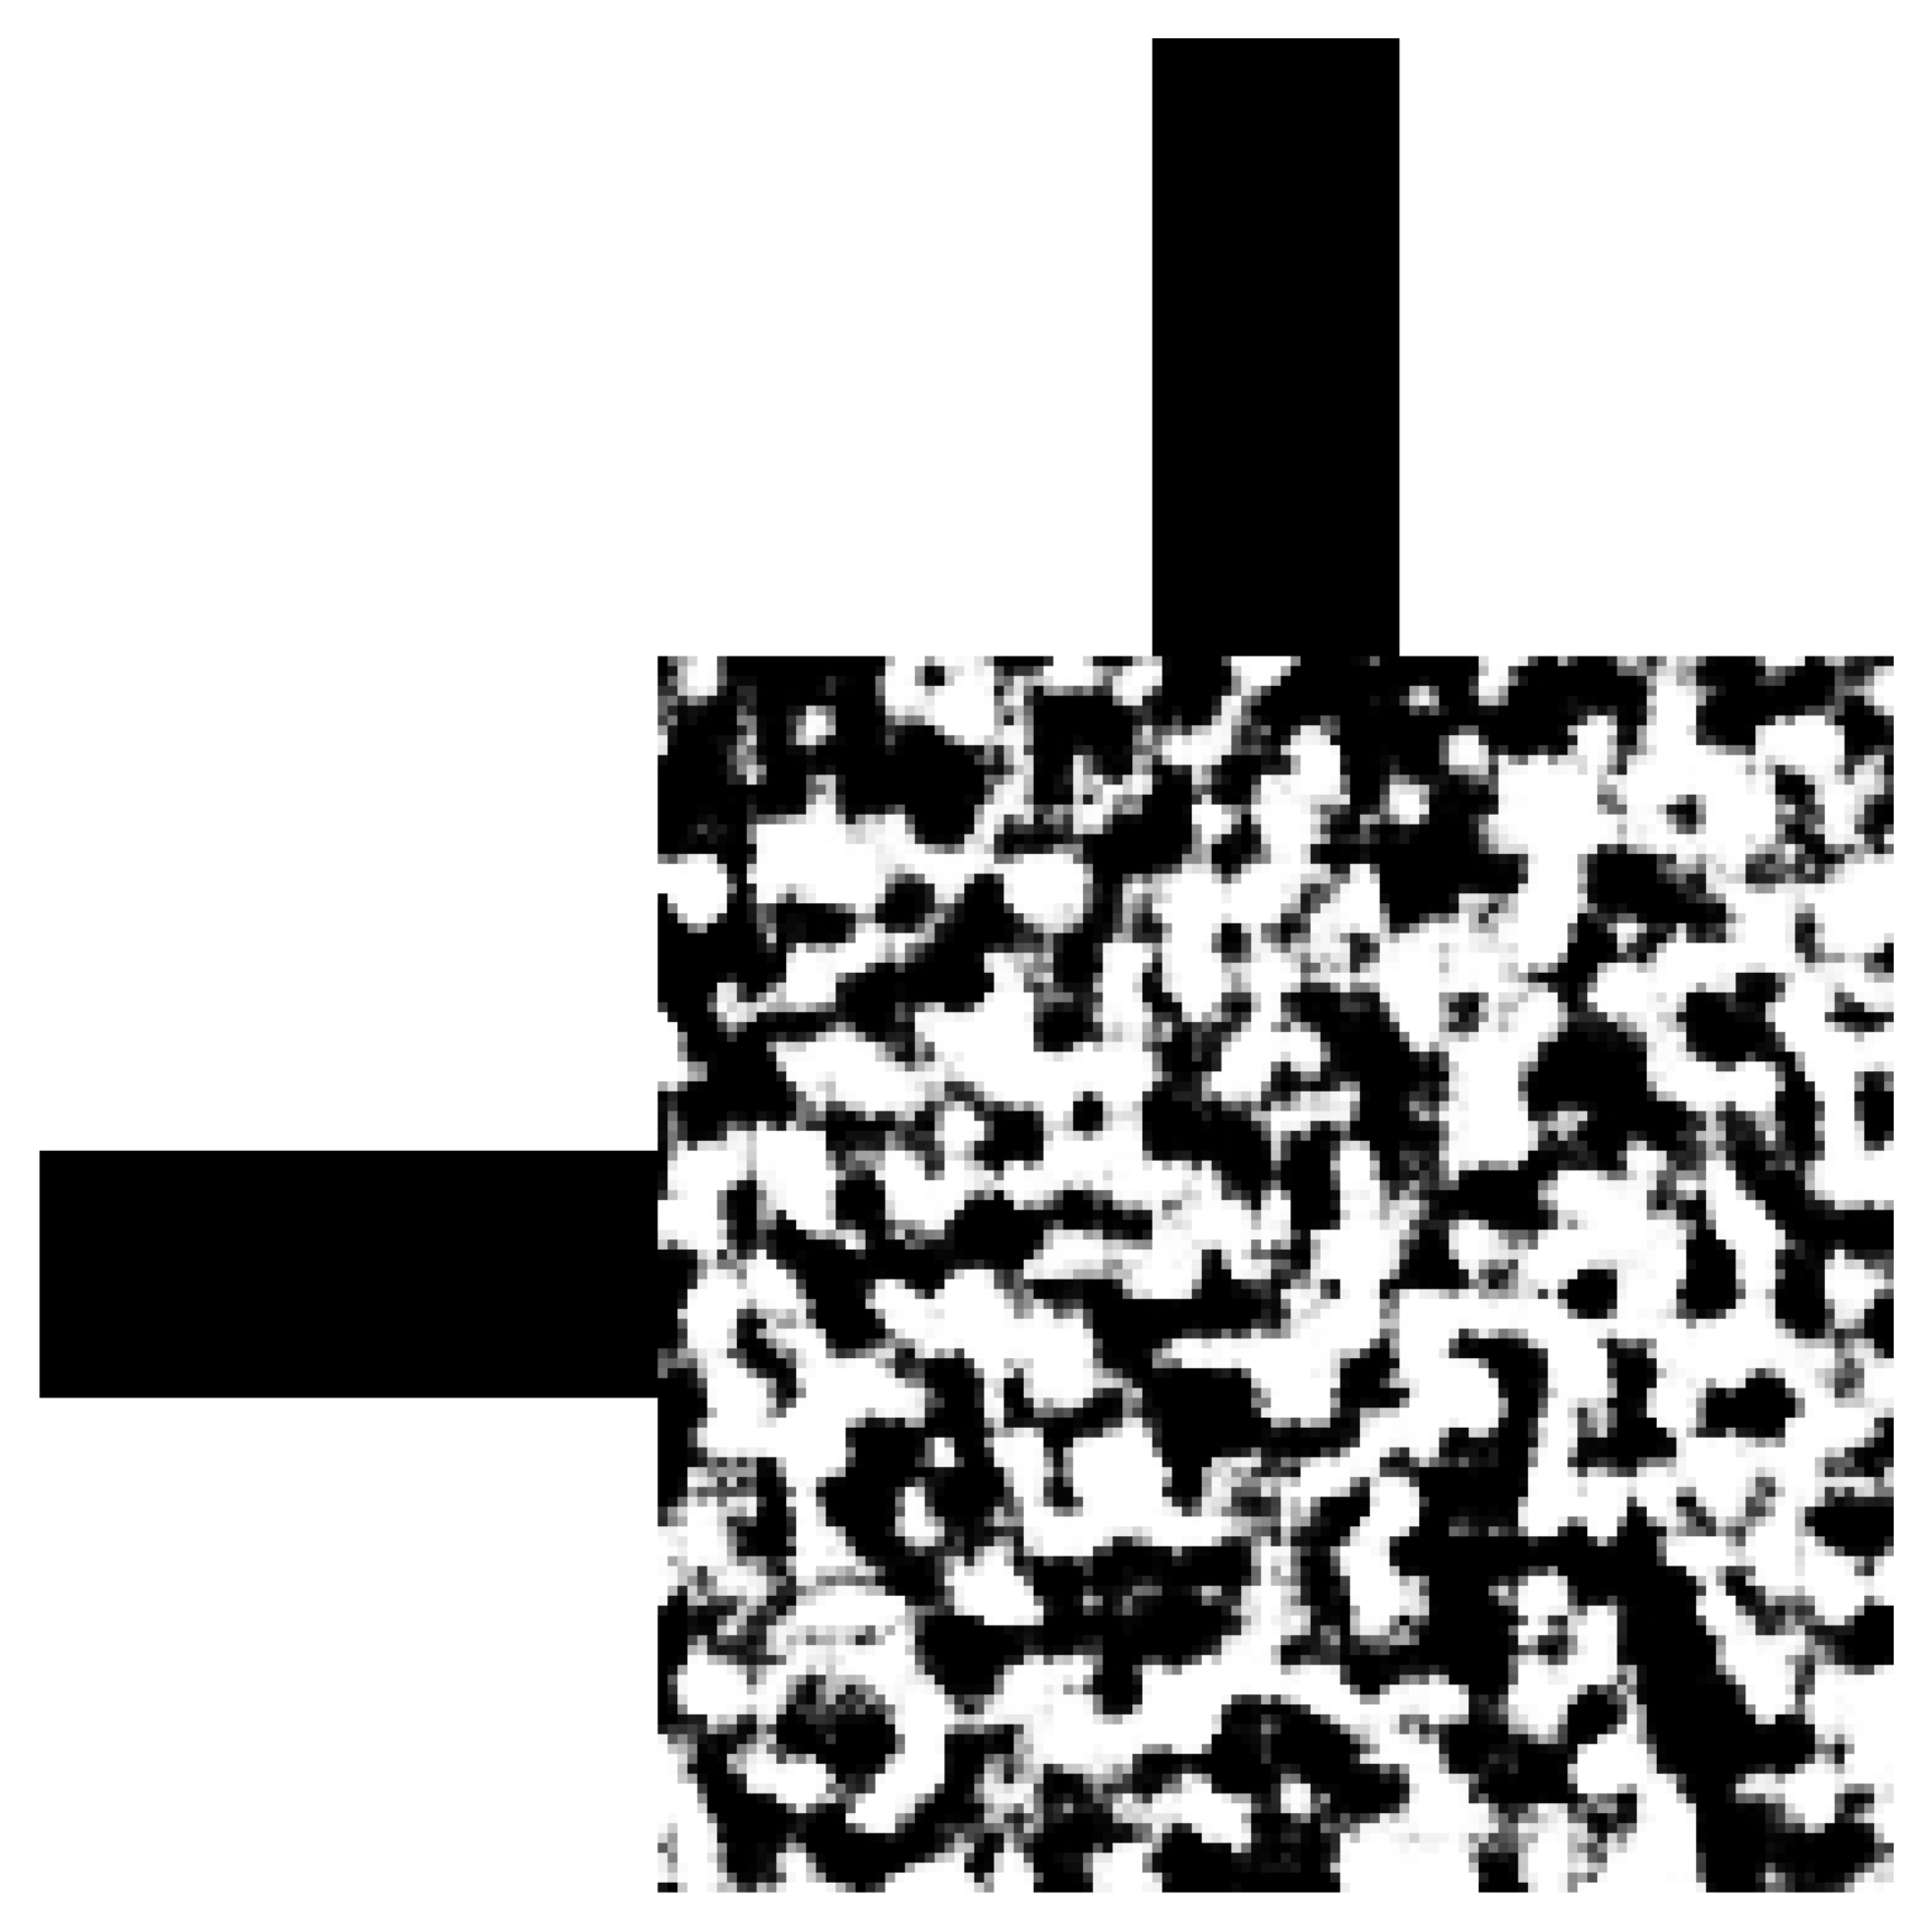
\includegraphics[width=0.20\textwidth]{image/results/bend/MMA/visualize_eps_fab_128.png} \\
      \cline{2-4}
      &
      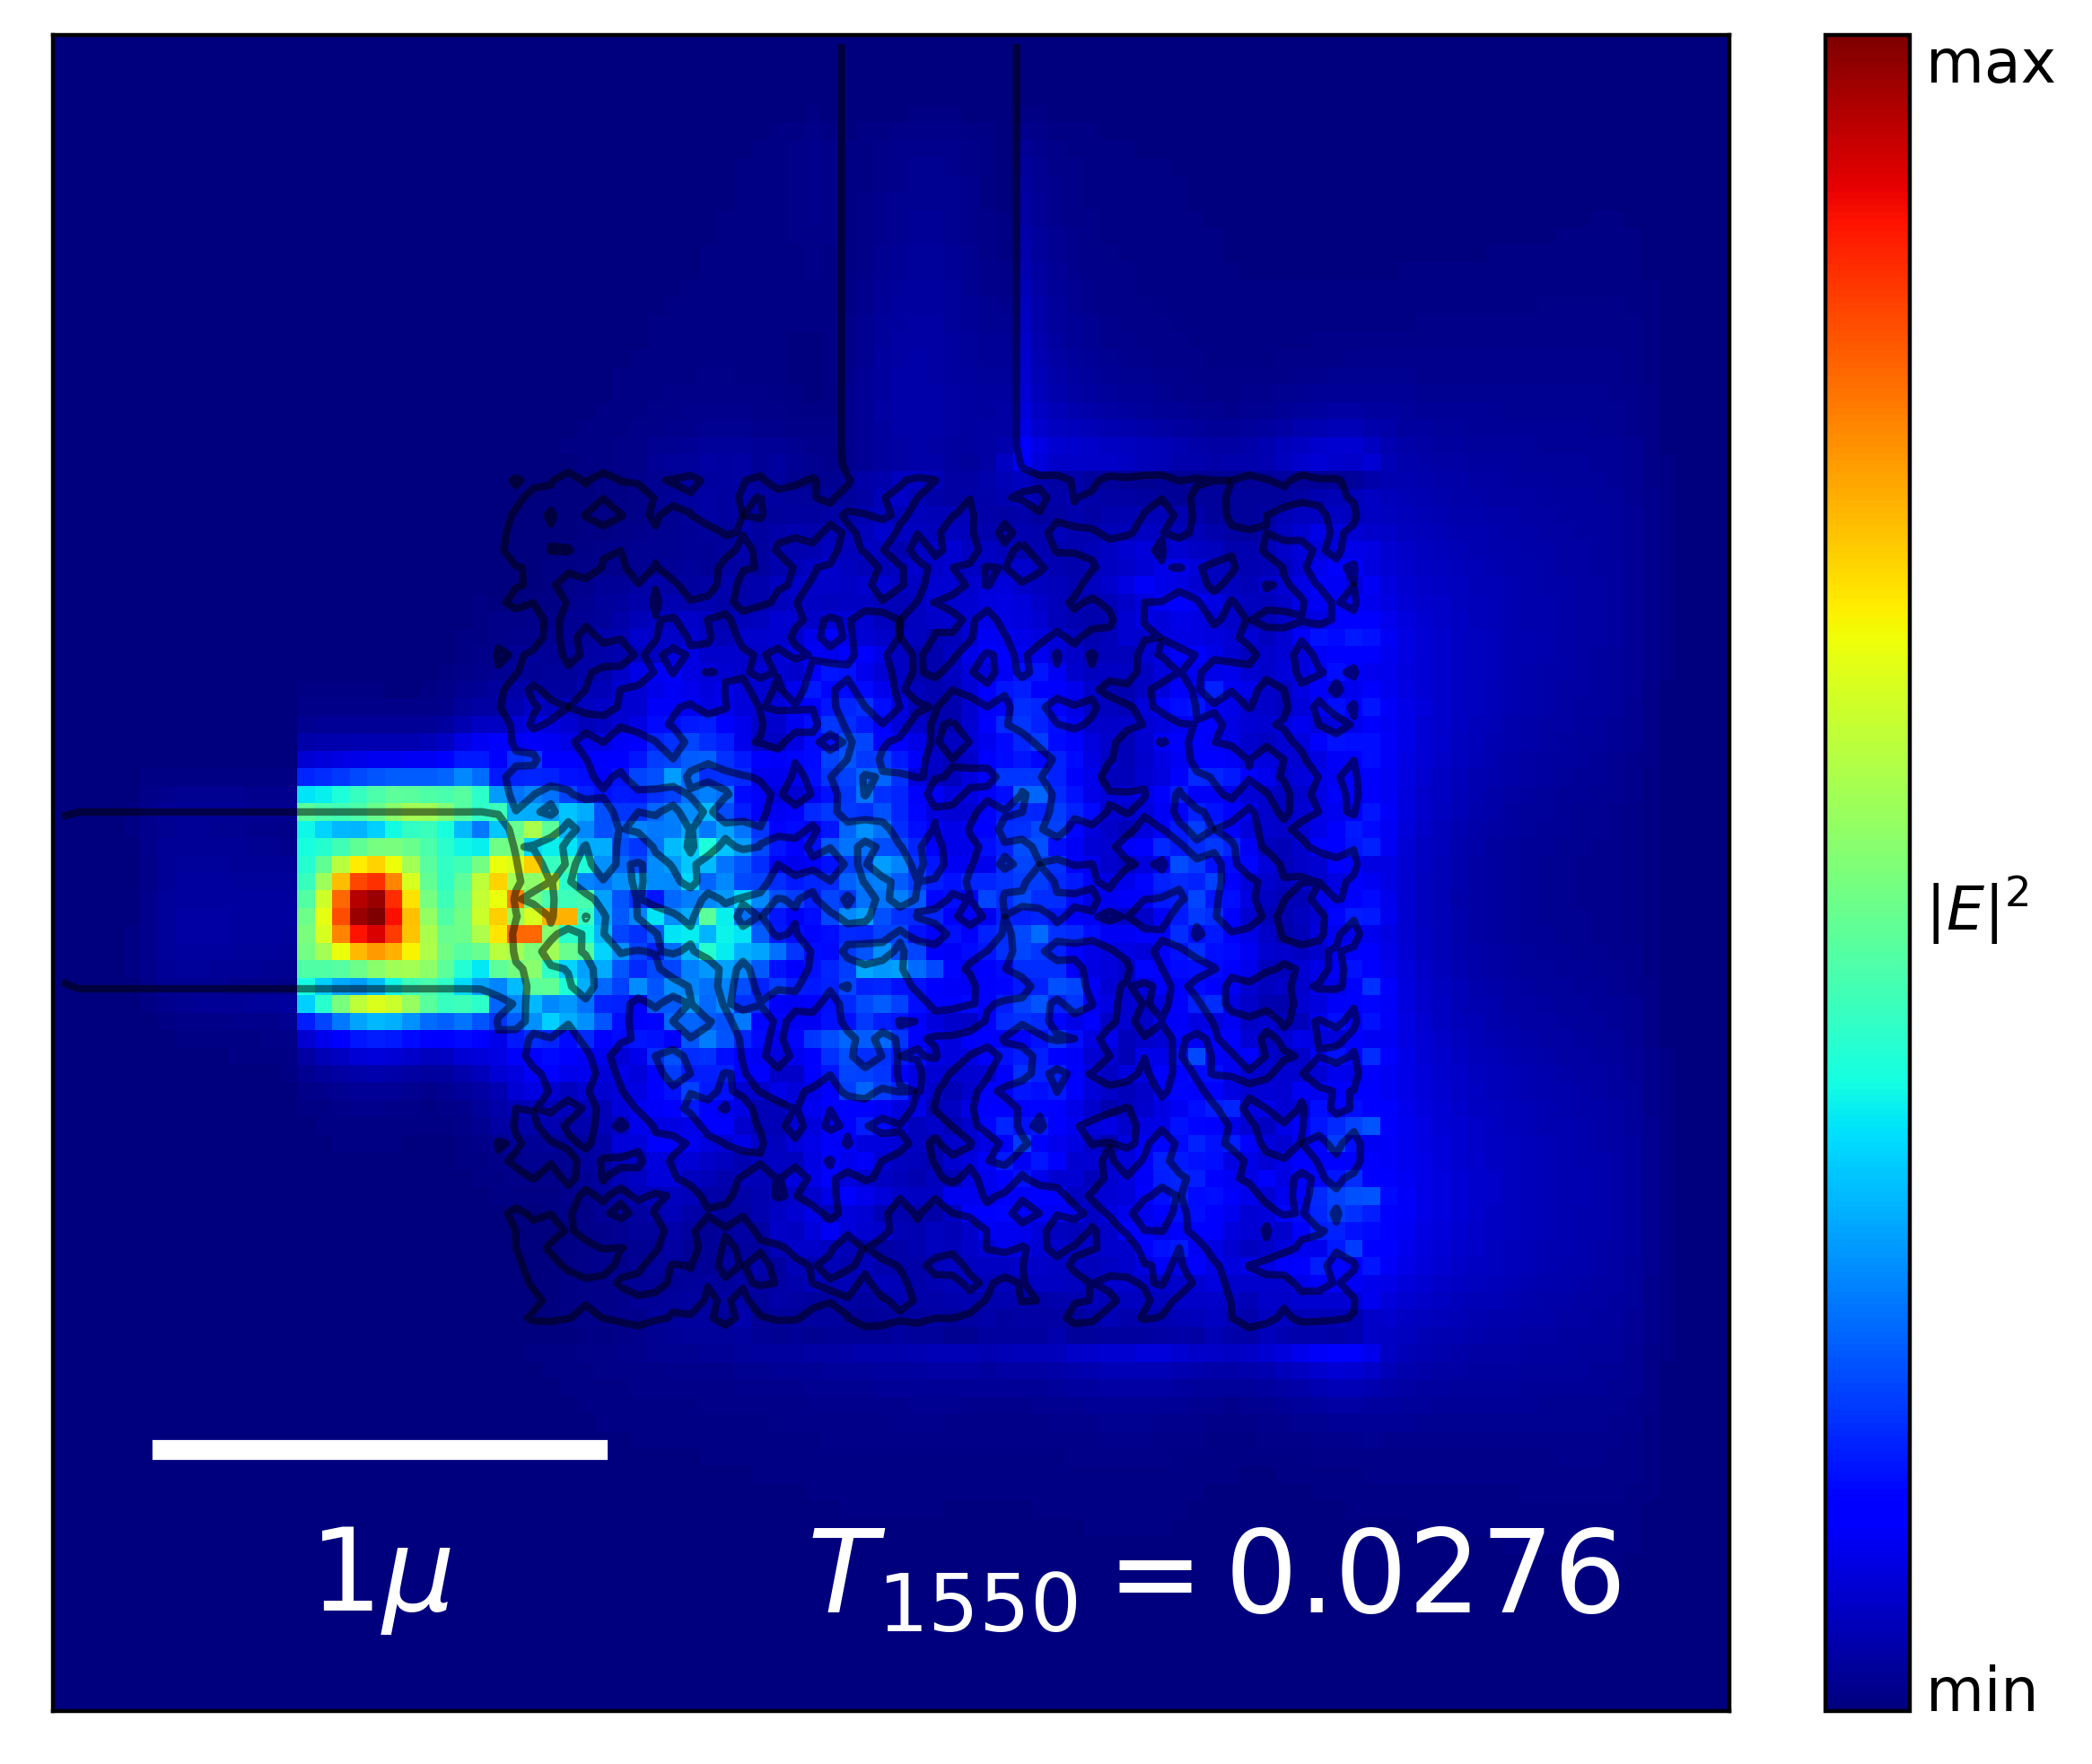
\includegraphics[width=0.33\textwidth]{image/results/bend/MMA/visualize_field_cont_128.png} &
      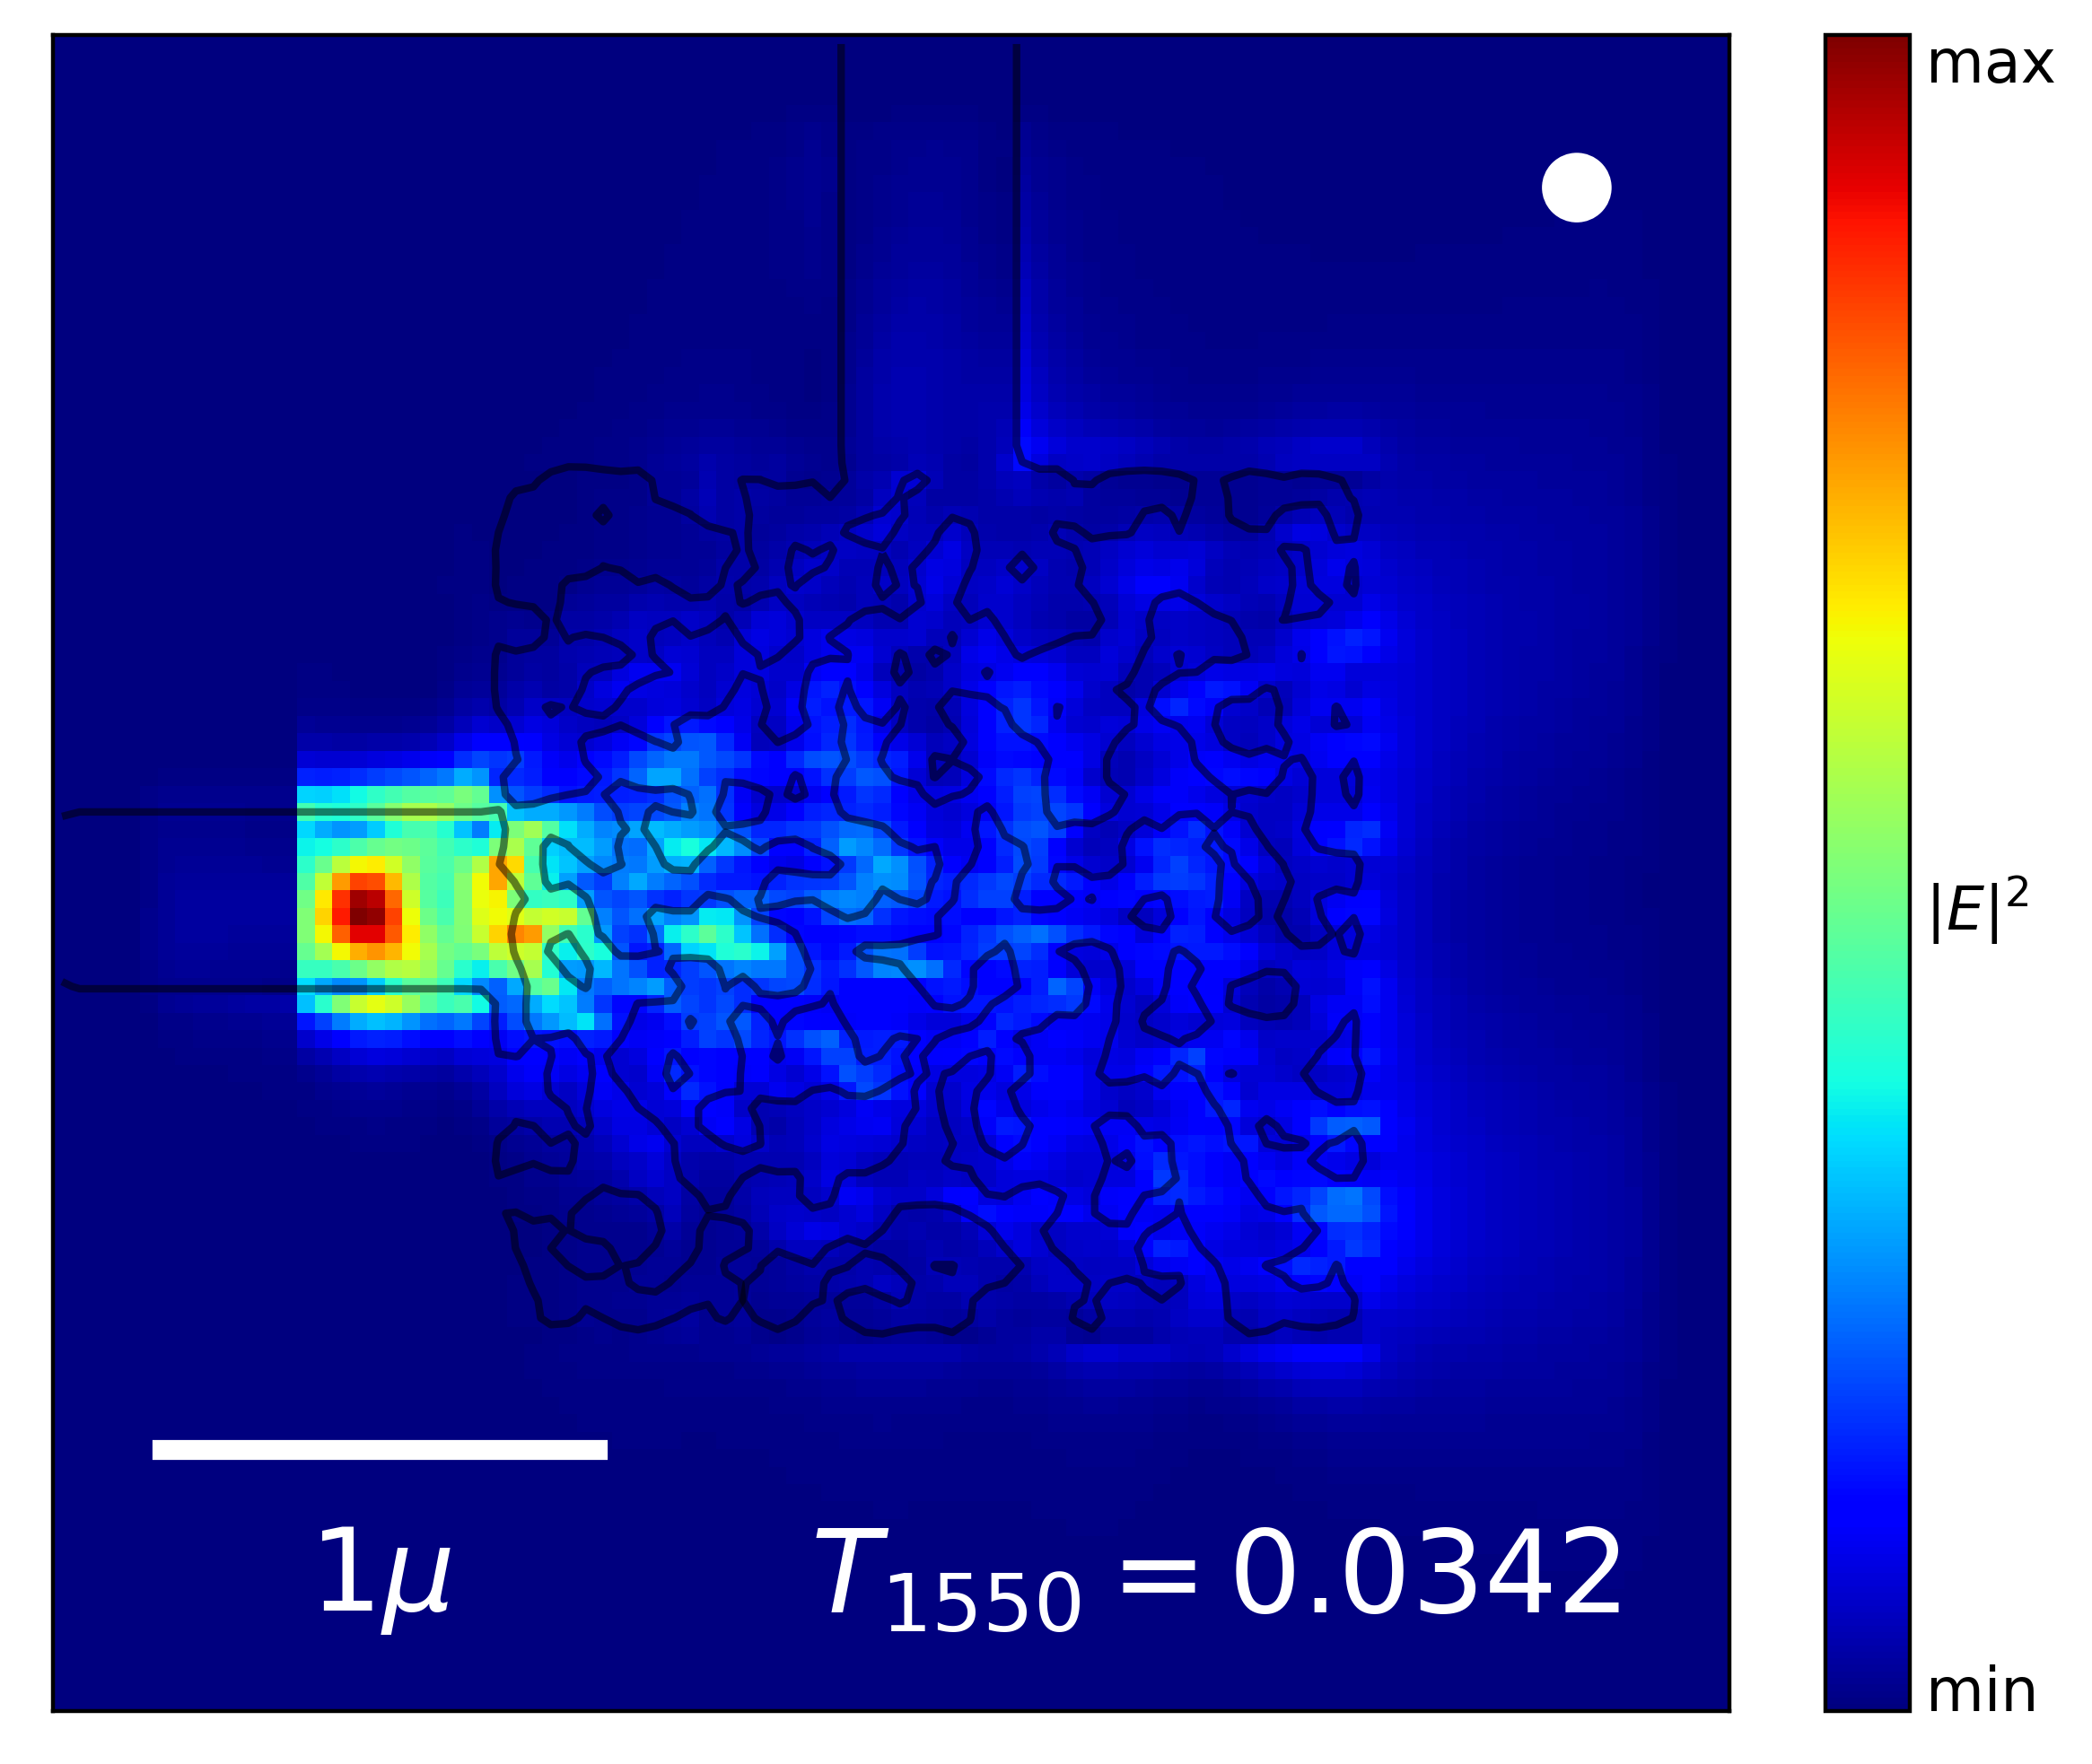
\includegraphics[width=0.33\textwidth]{image/results/bend/MMA/visualize_field_disc_128.png} &
      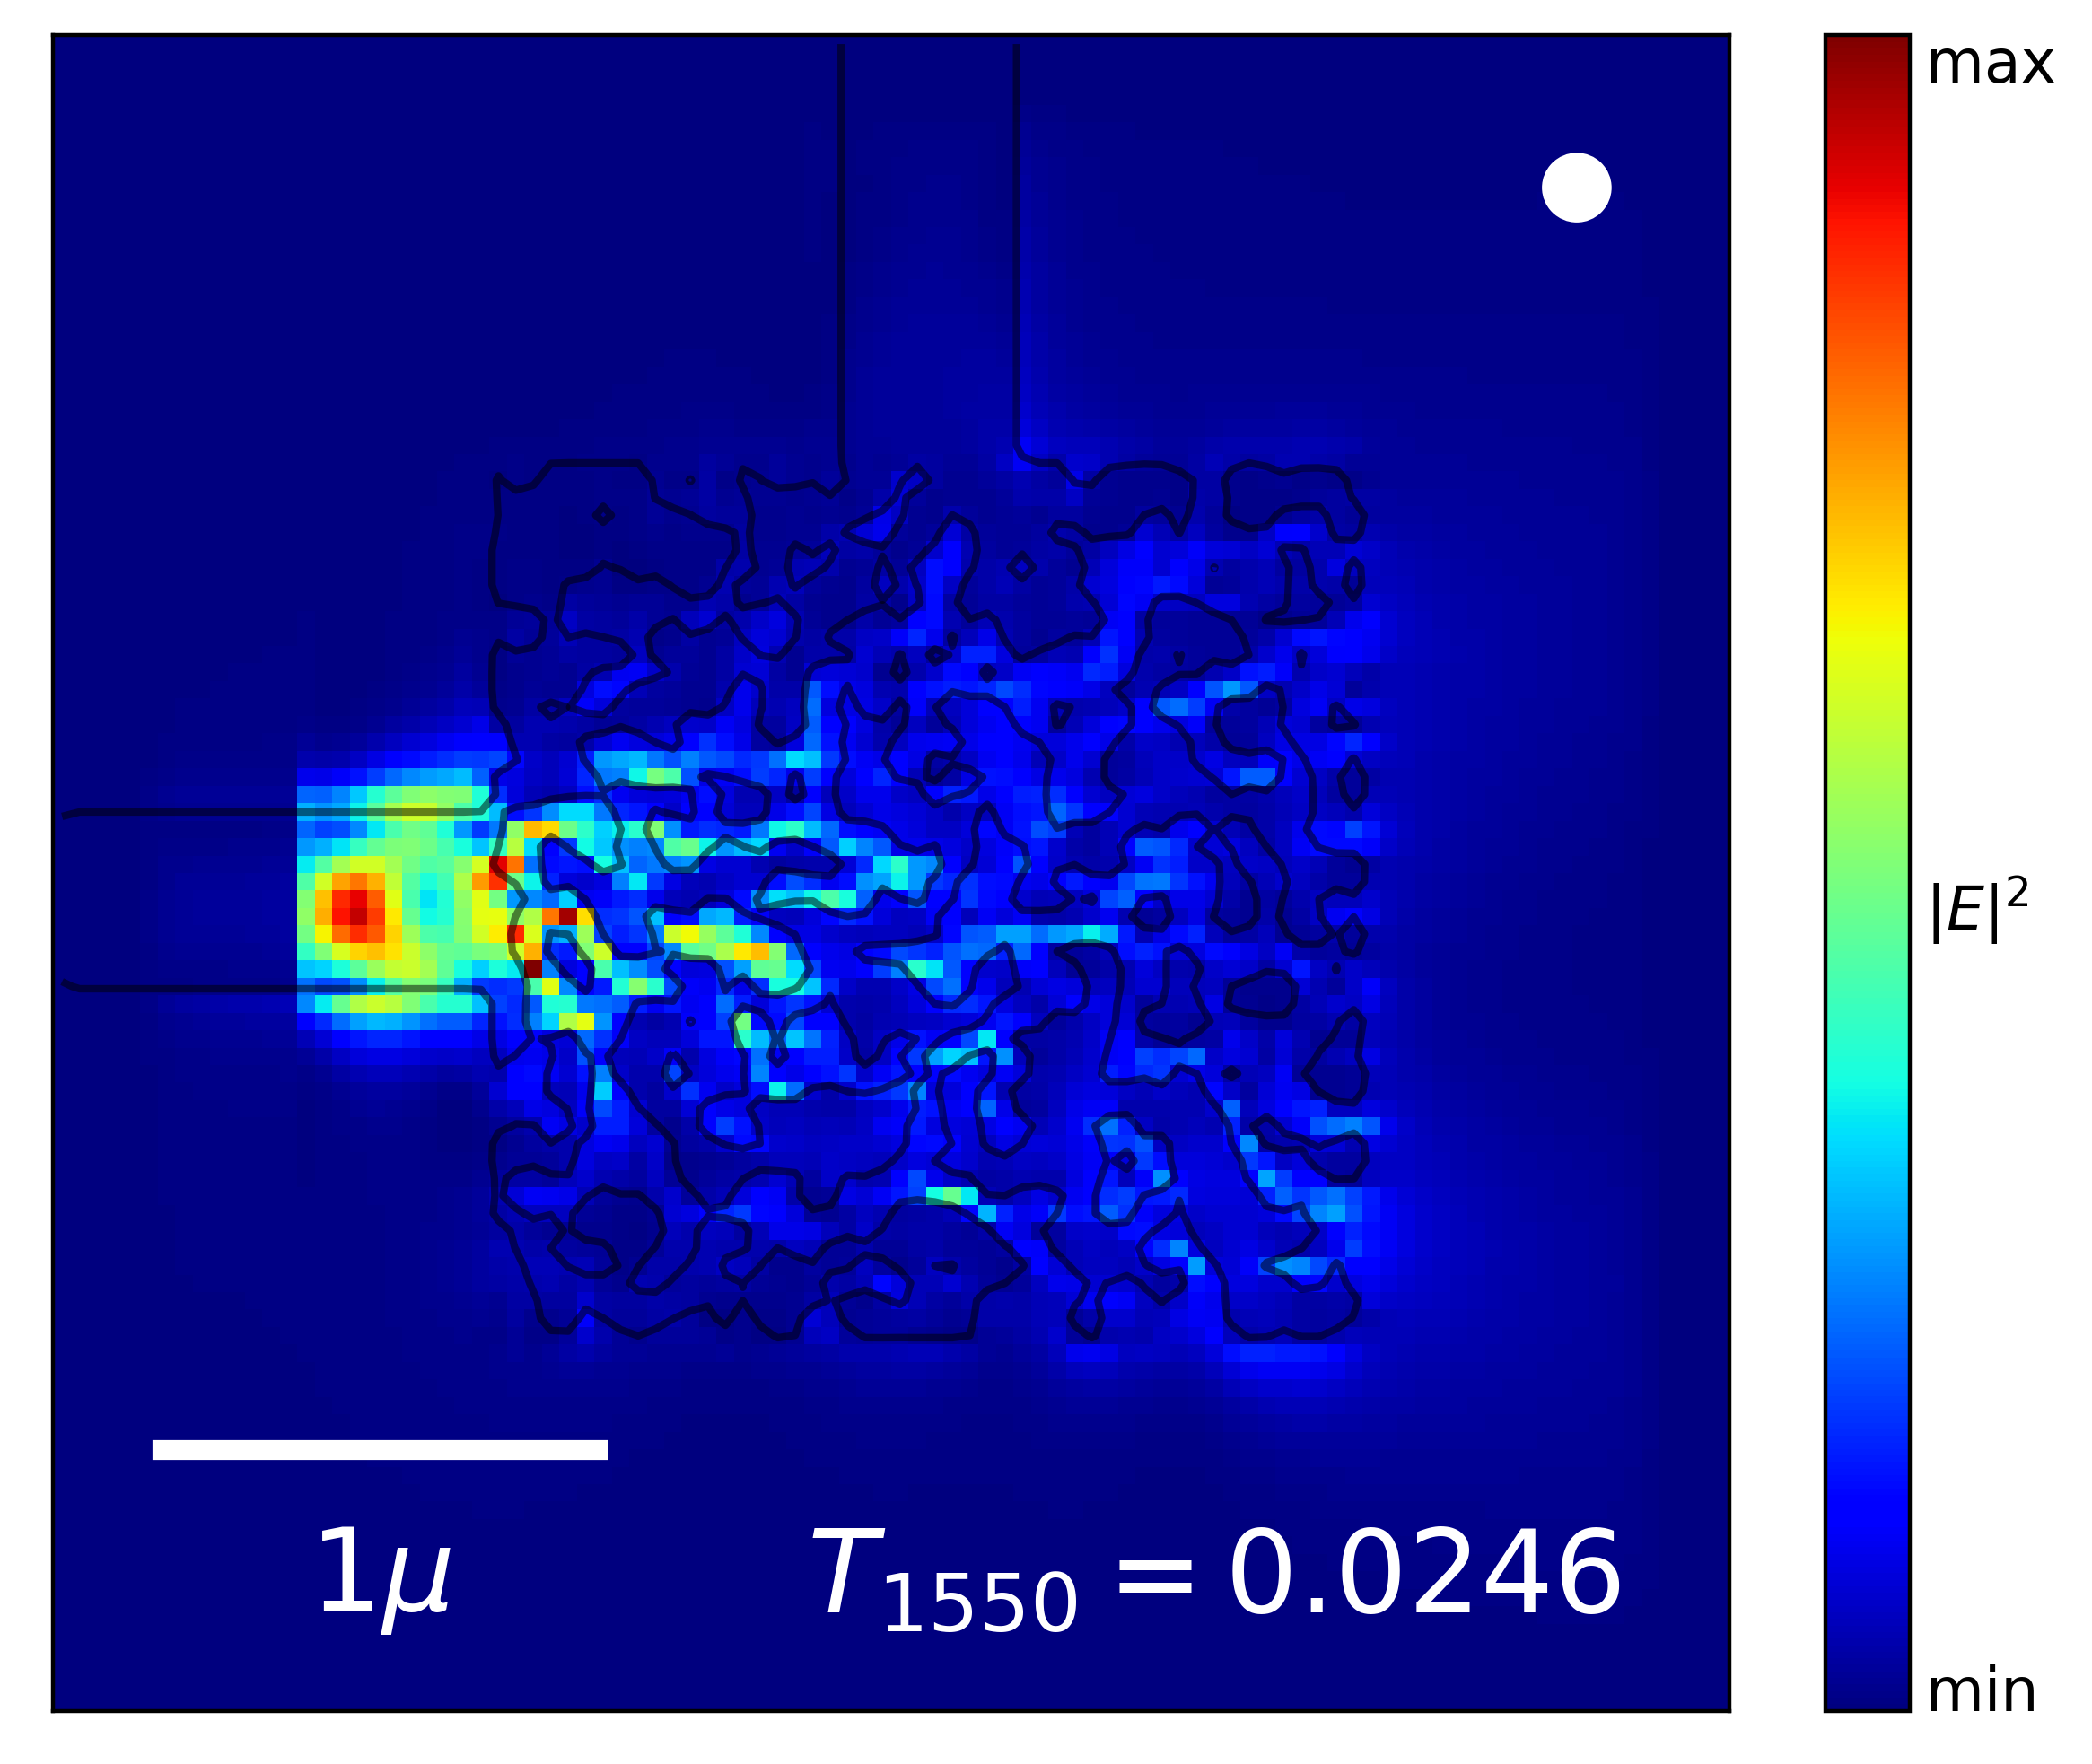
\includegraphics[width=0.33\textwidth]{image/results/bend/MMA/visualize_field_fab_128.png} \\
    \hline
      \multirow{2}{*}{256} &
      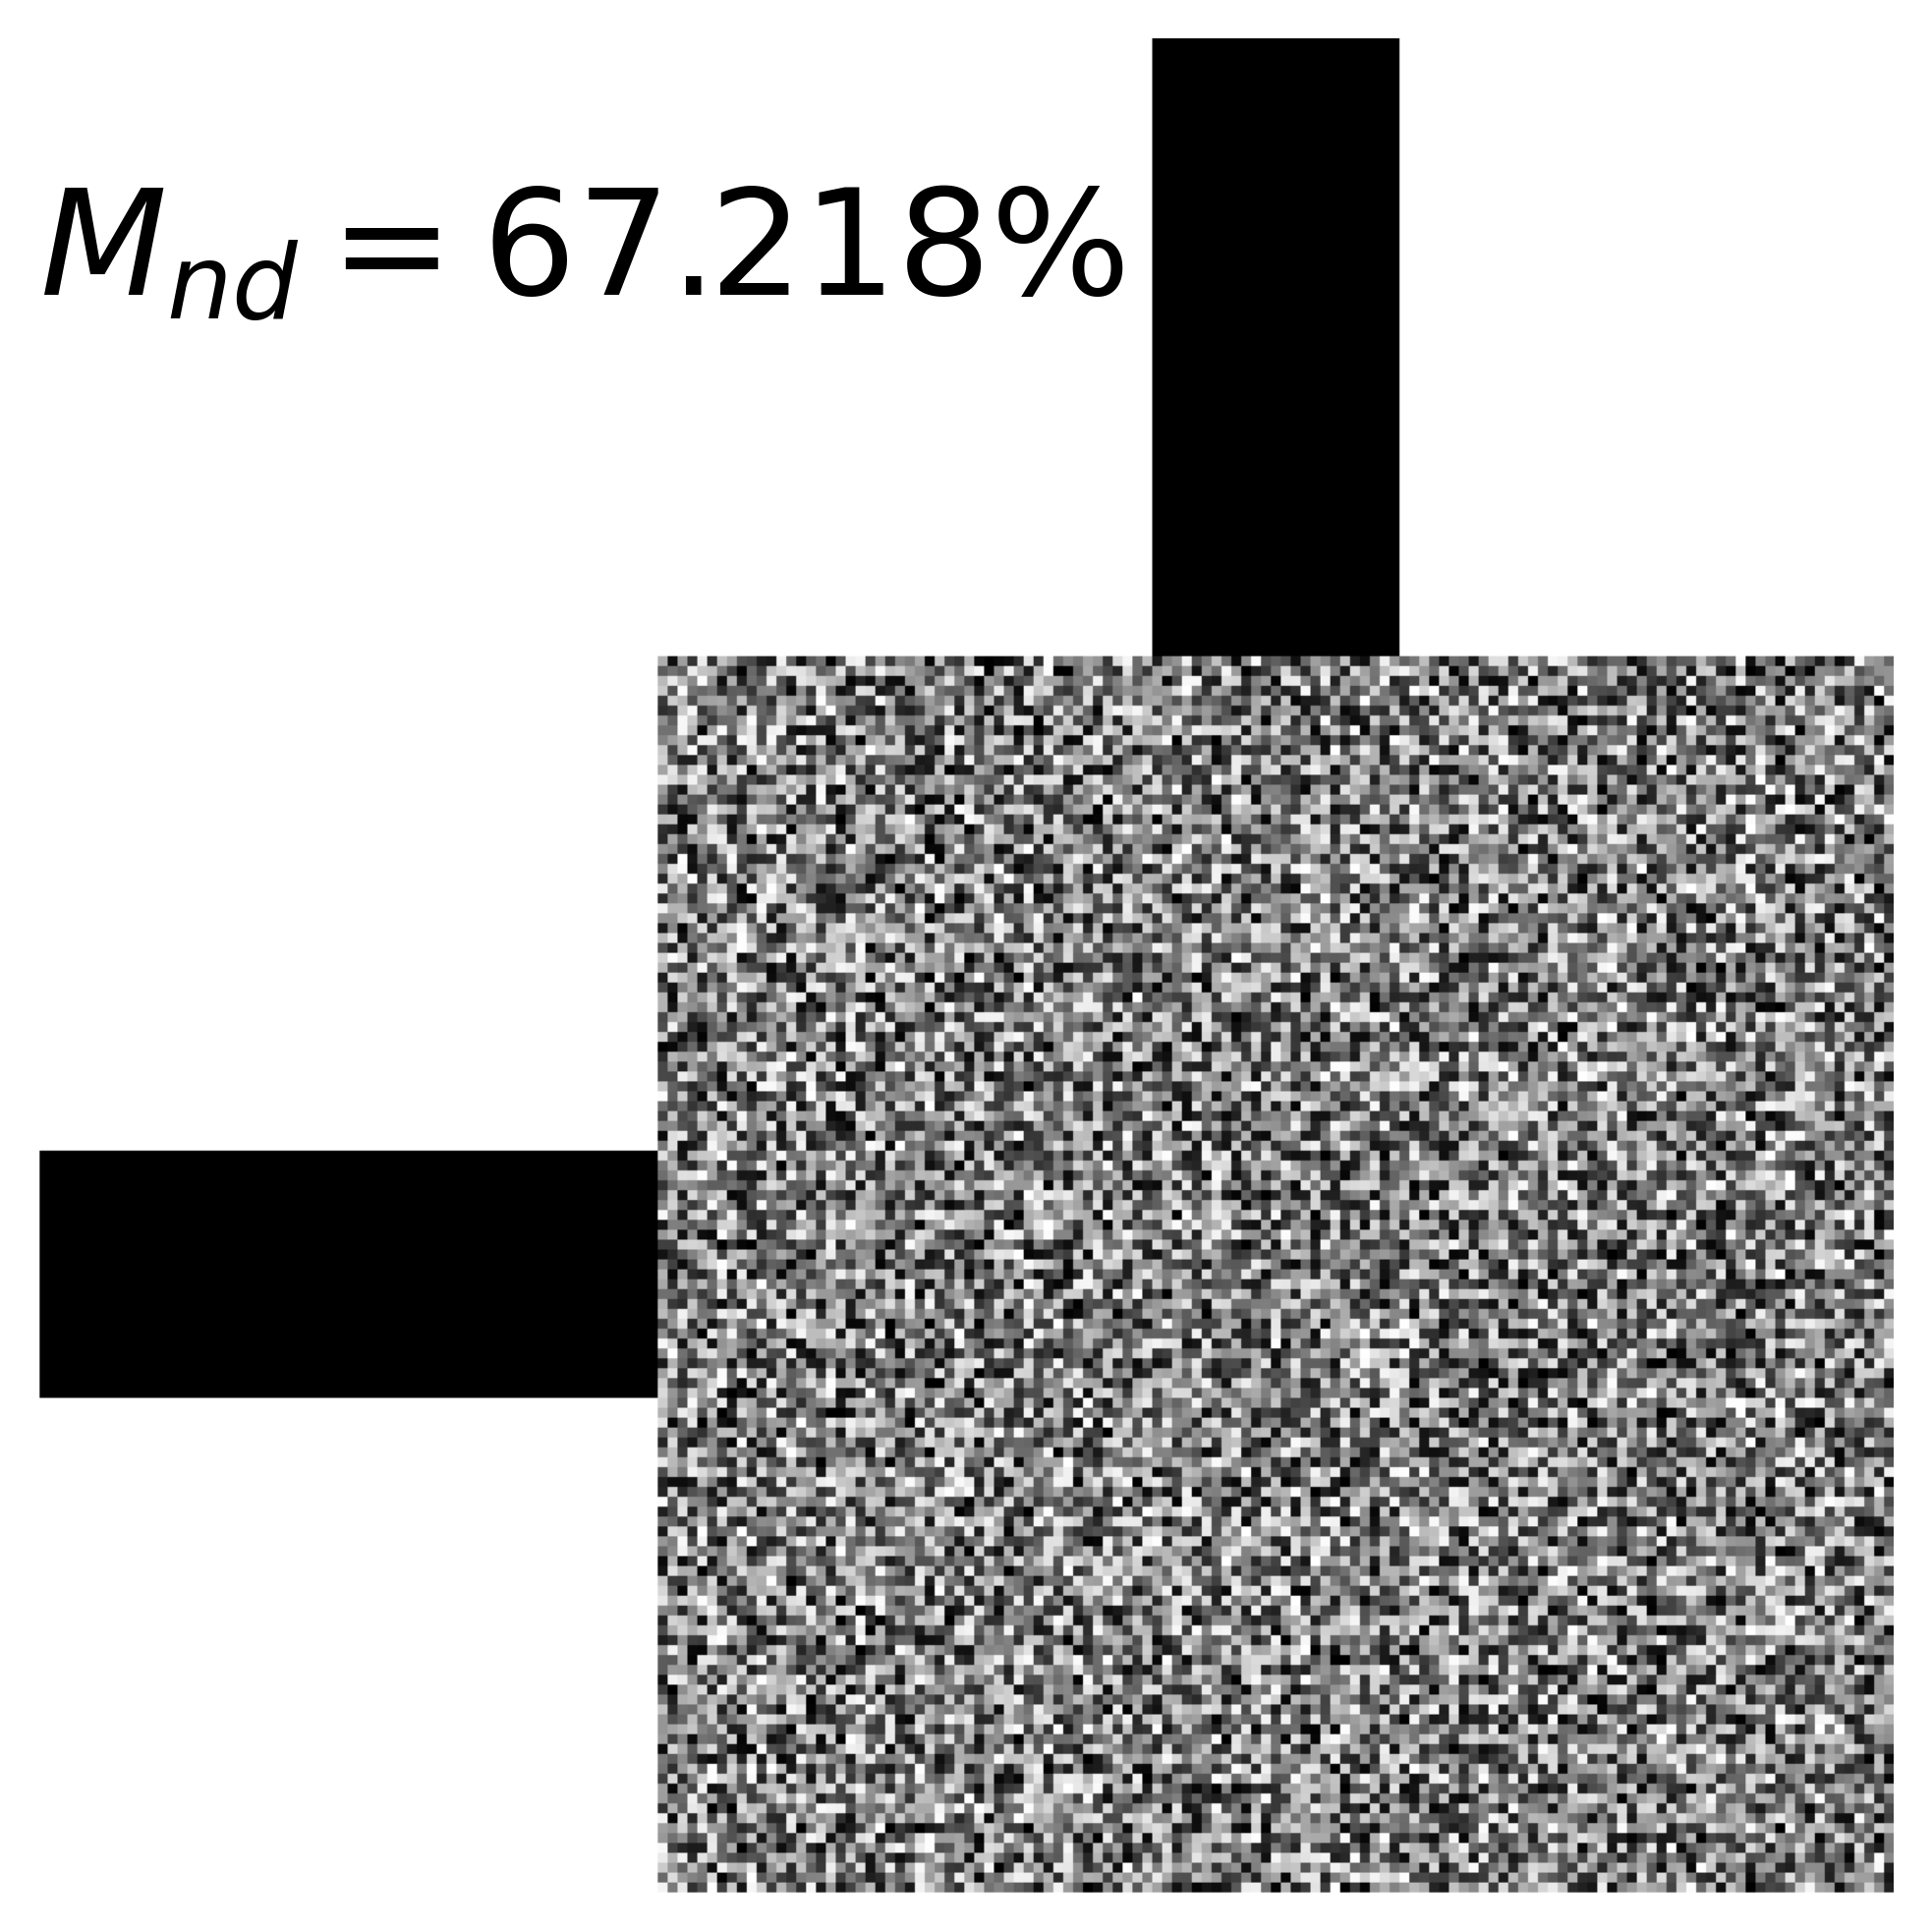
\includegraphics[width=0.20\textwidth]{image/results/bend/MMA/visualize_eps_cont_256.png} &
      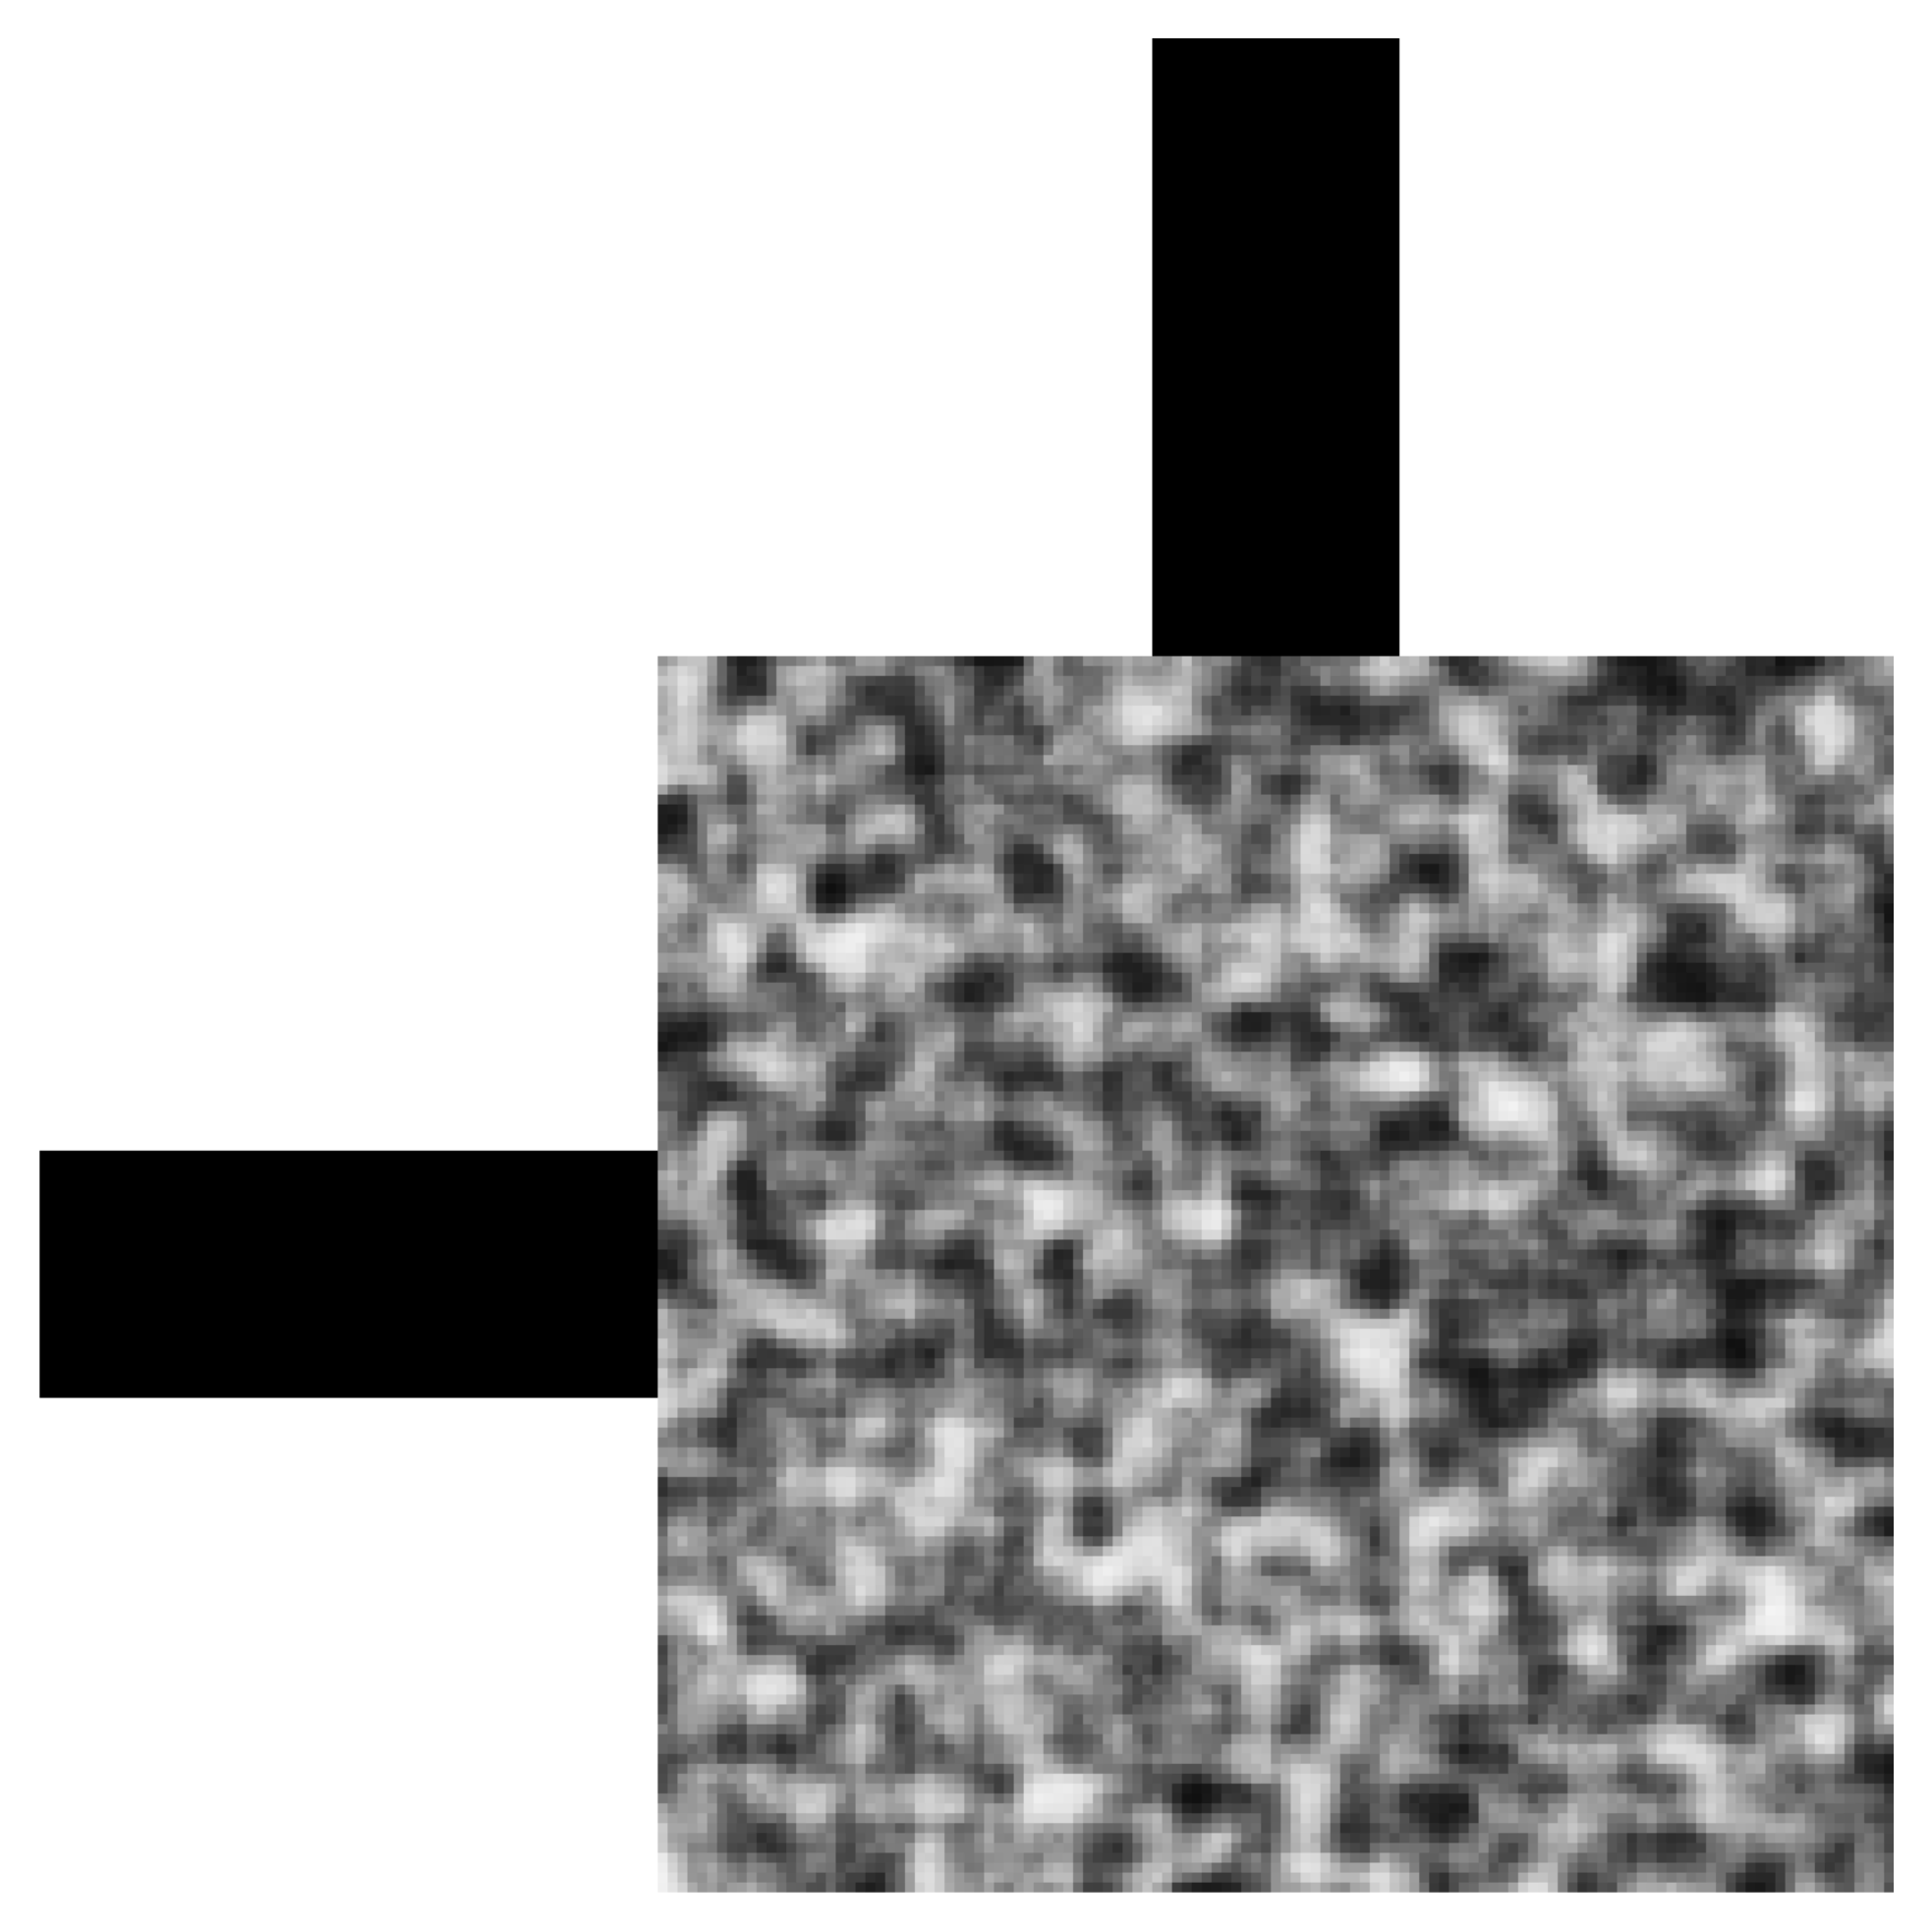
\includegraphics[width=0.20\textwidth]{image/results/bend/MMA/visualize_eps_disc_256.png} &
      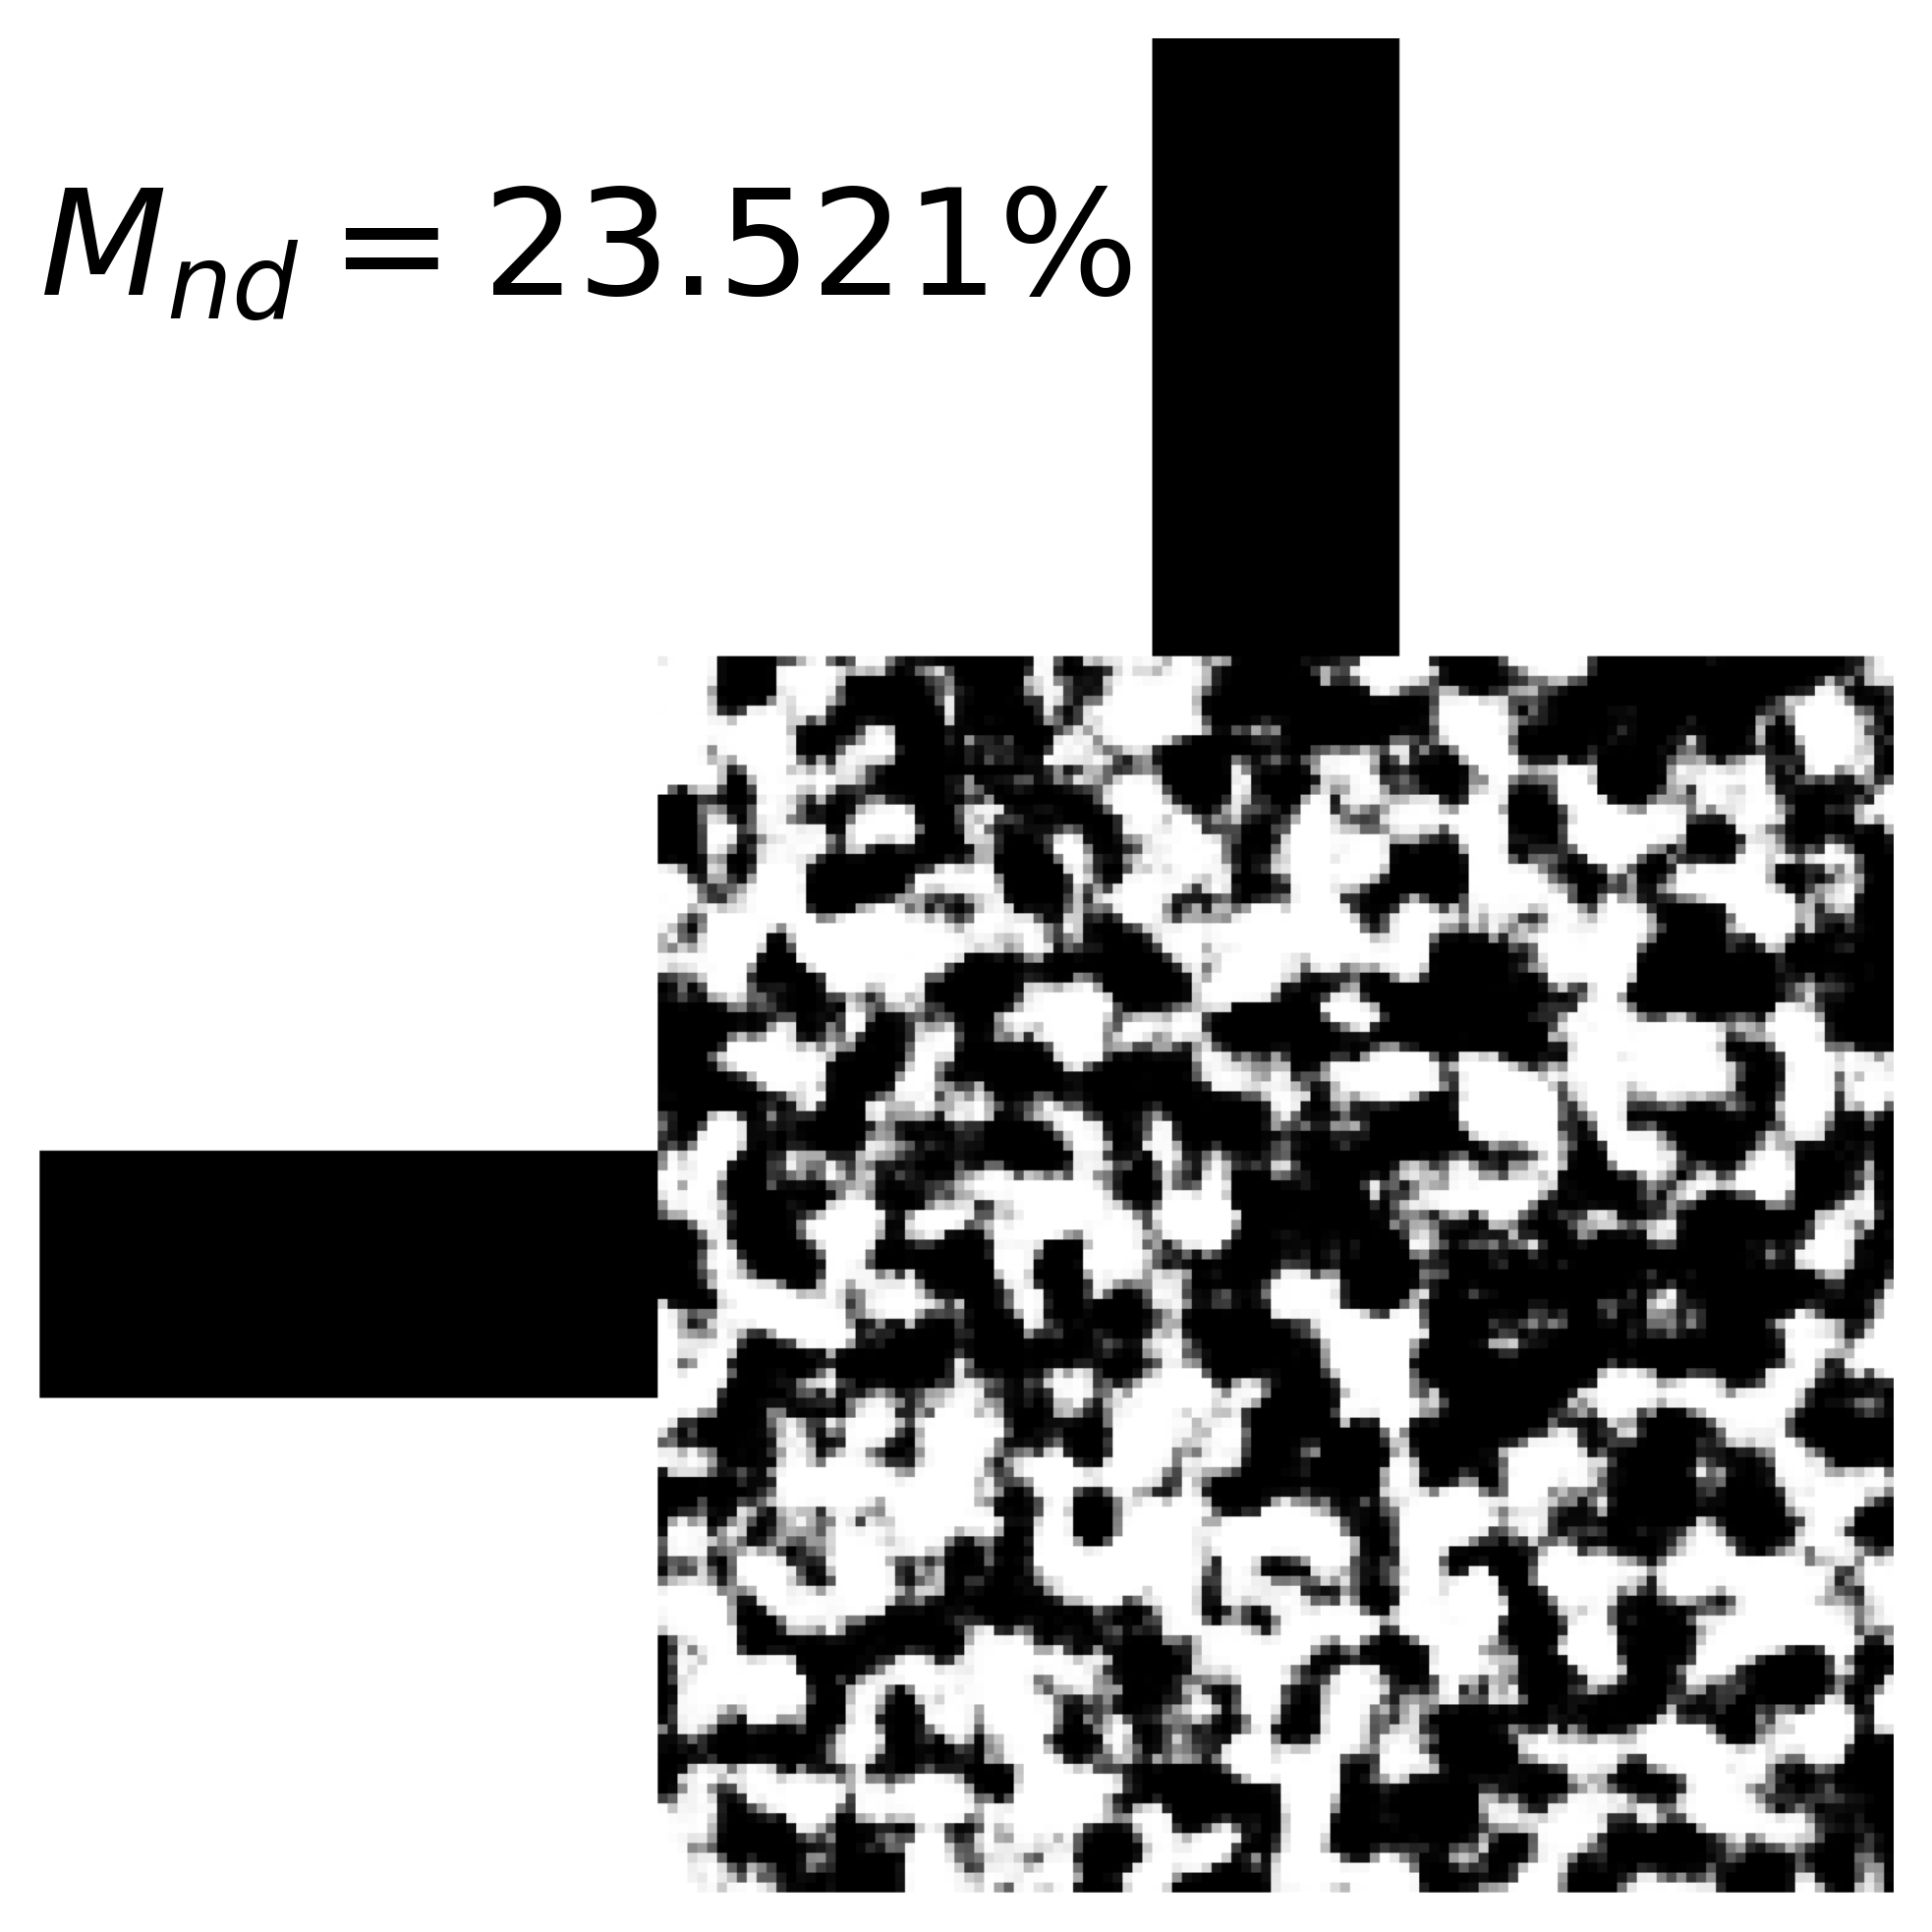
\includegraphics[width=0.20\textwidth]{image/results/bend/MMA/visualize_eps_fab_256.png} \\
      \cline{2-4}
      &
      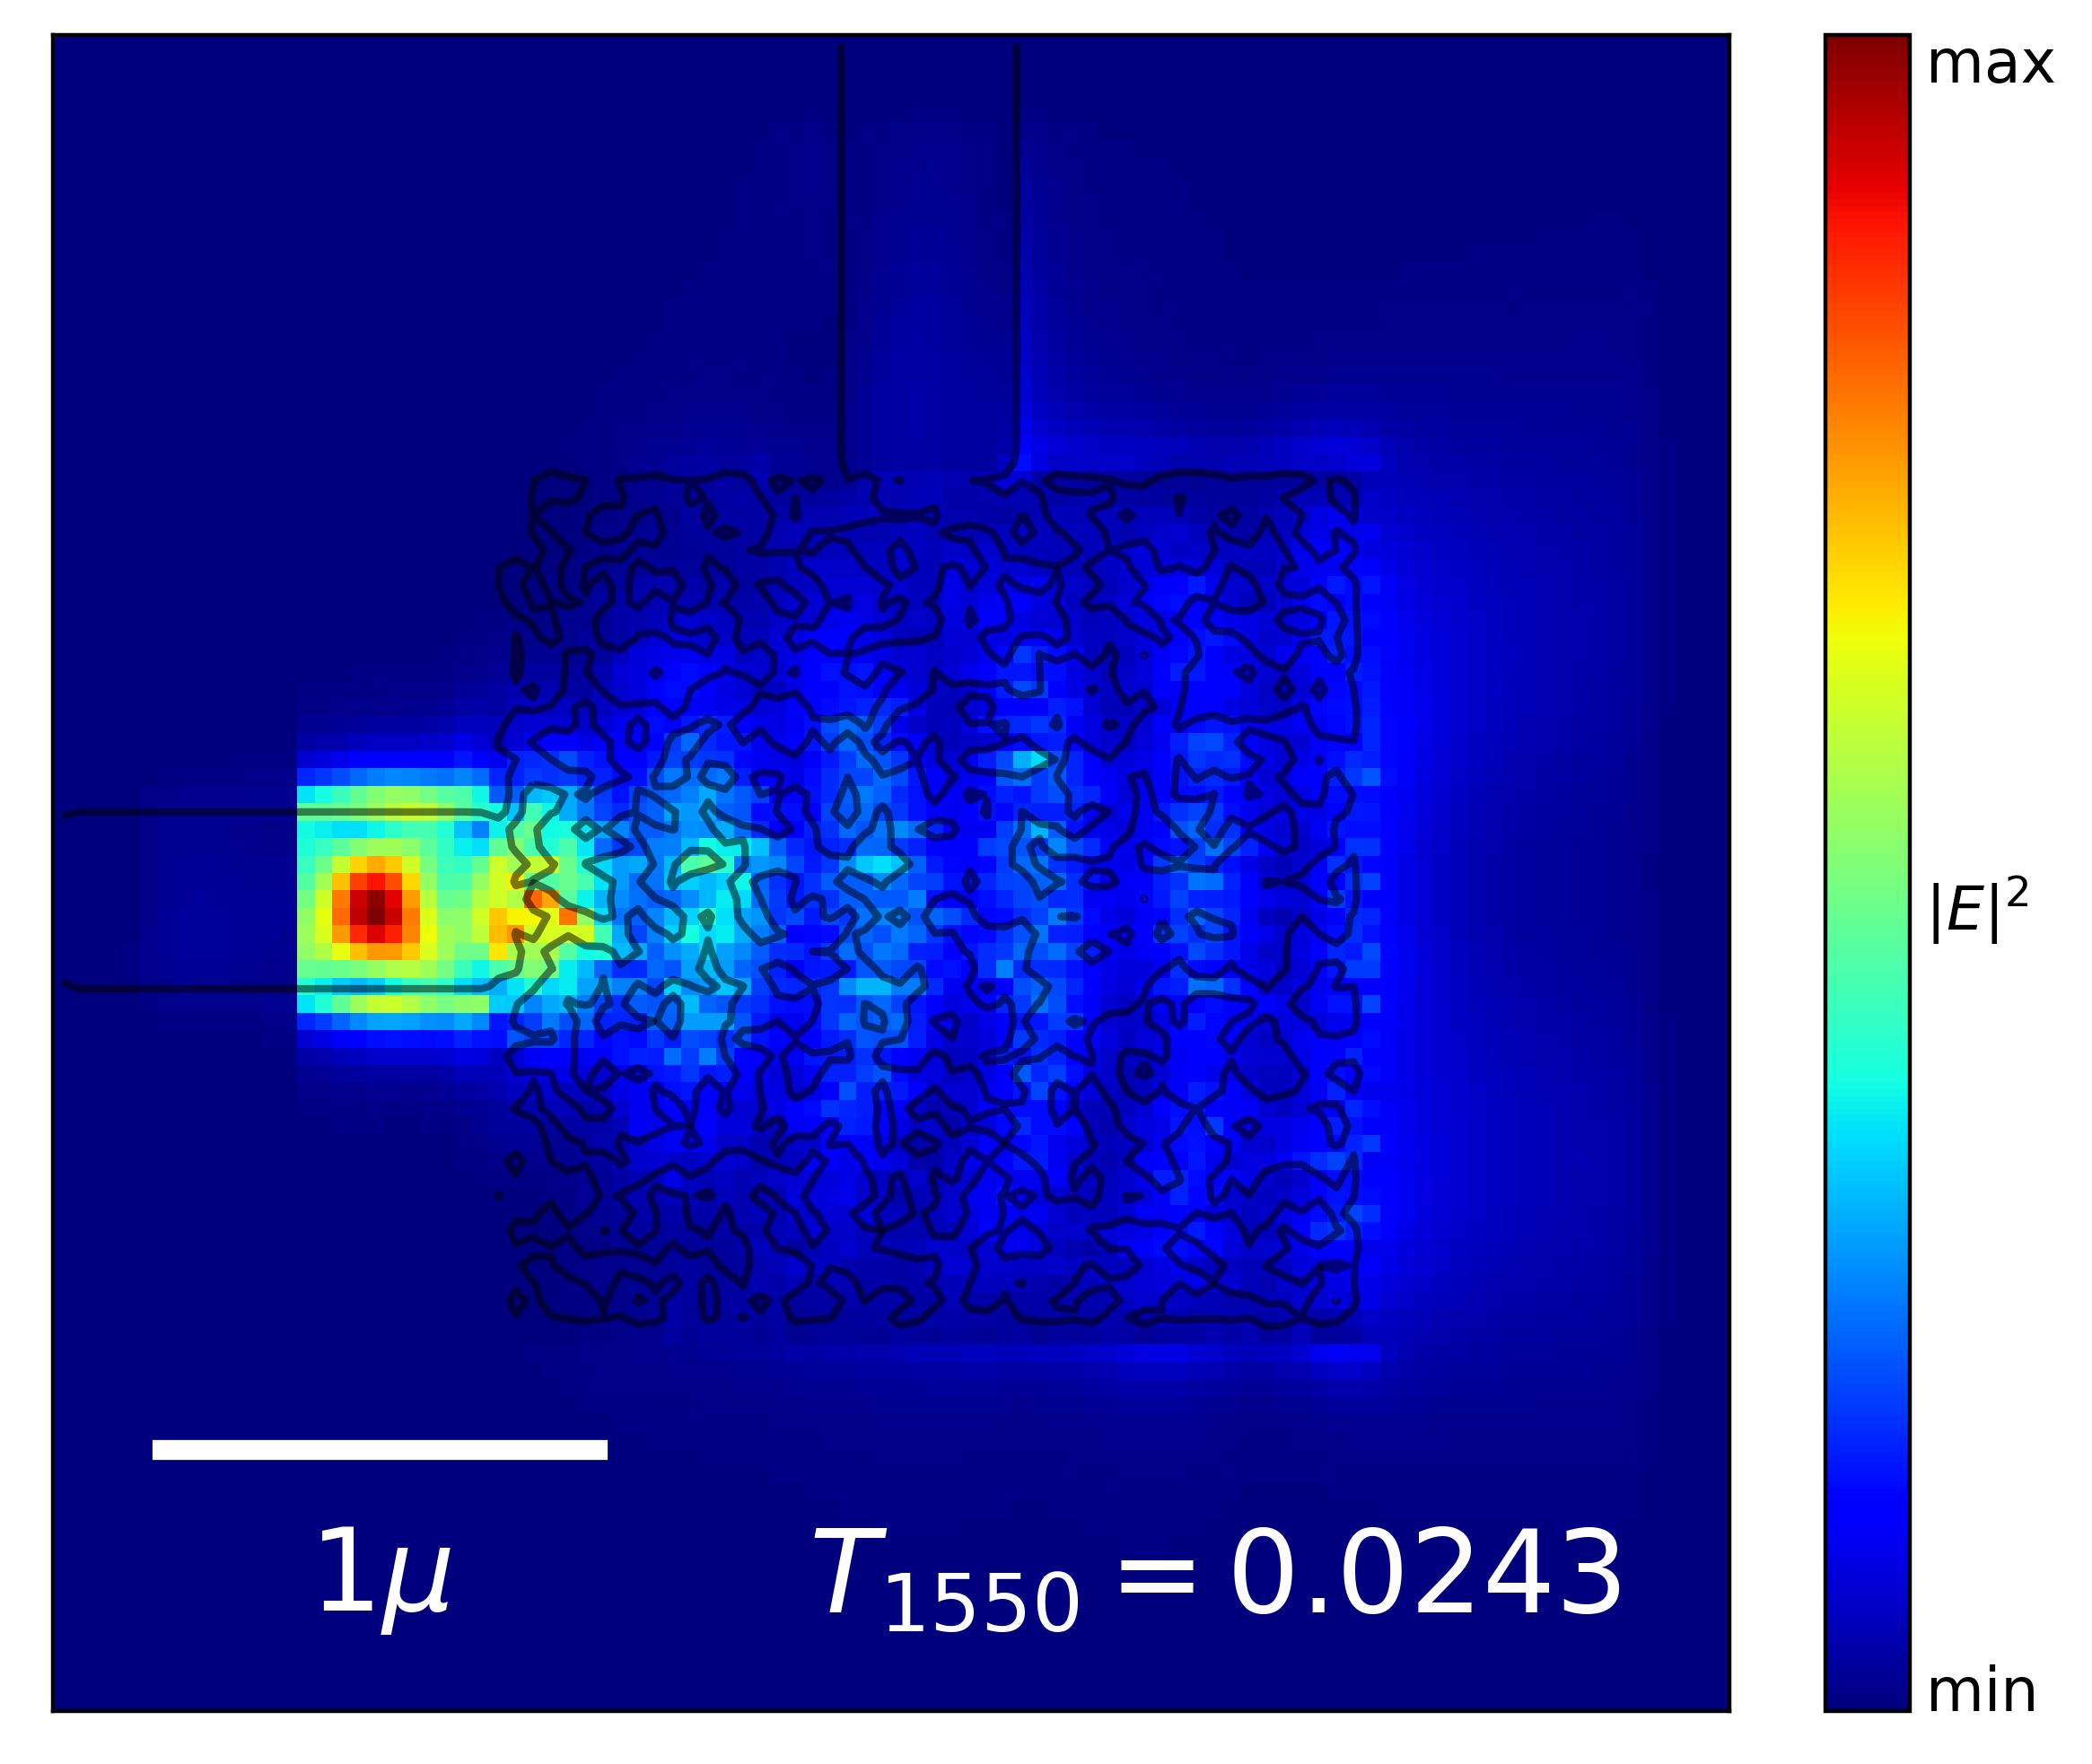
\includegraphics[width=0.33\textwidth]{image/results/bend/MMA/visualize_field_cont_256.png} &
      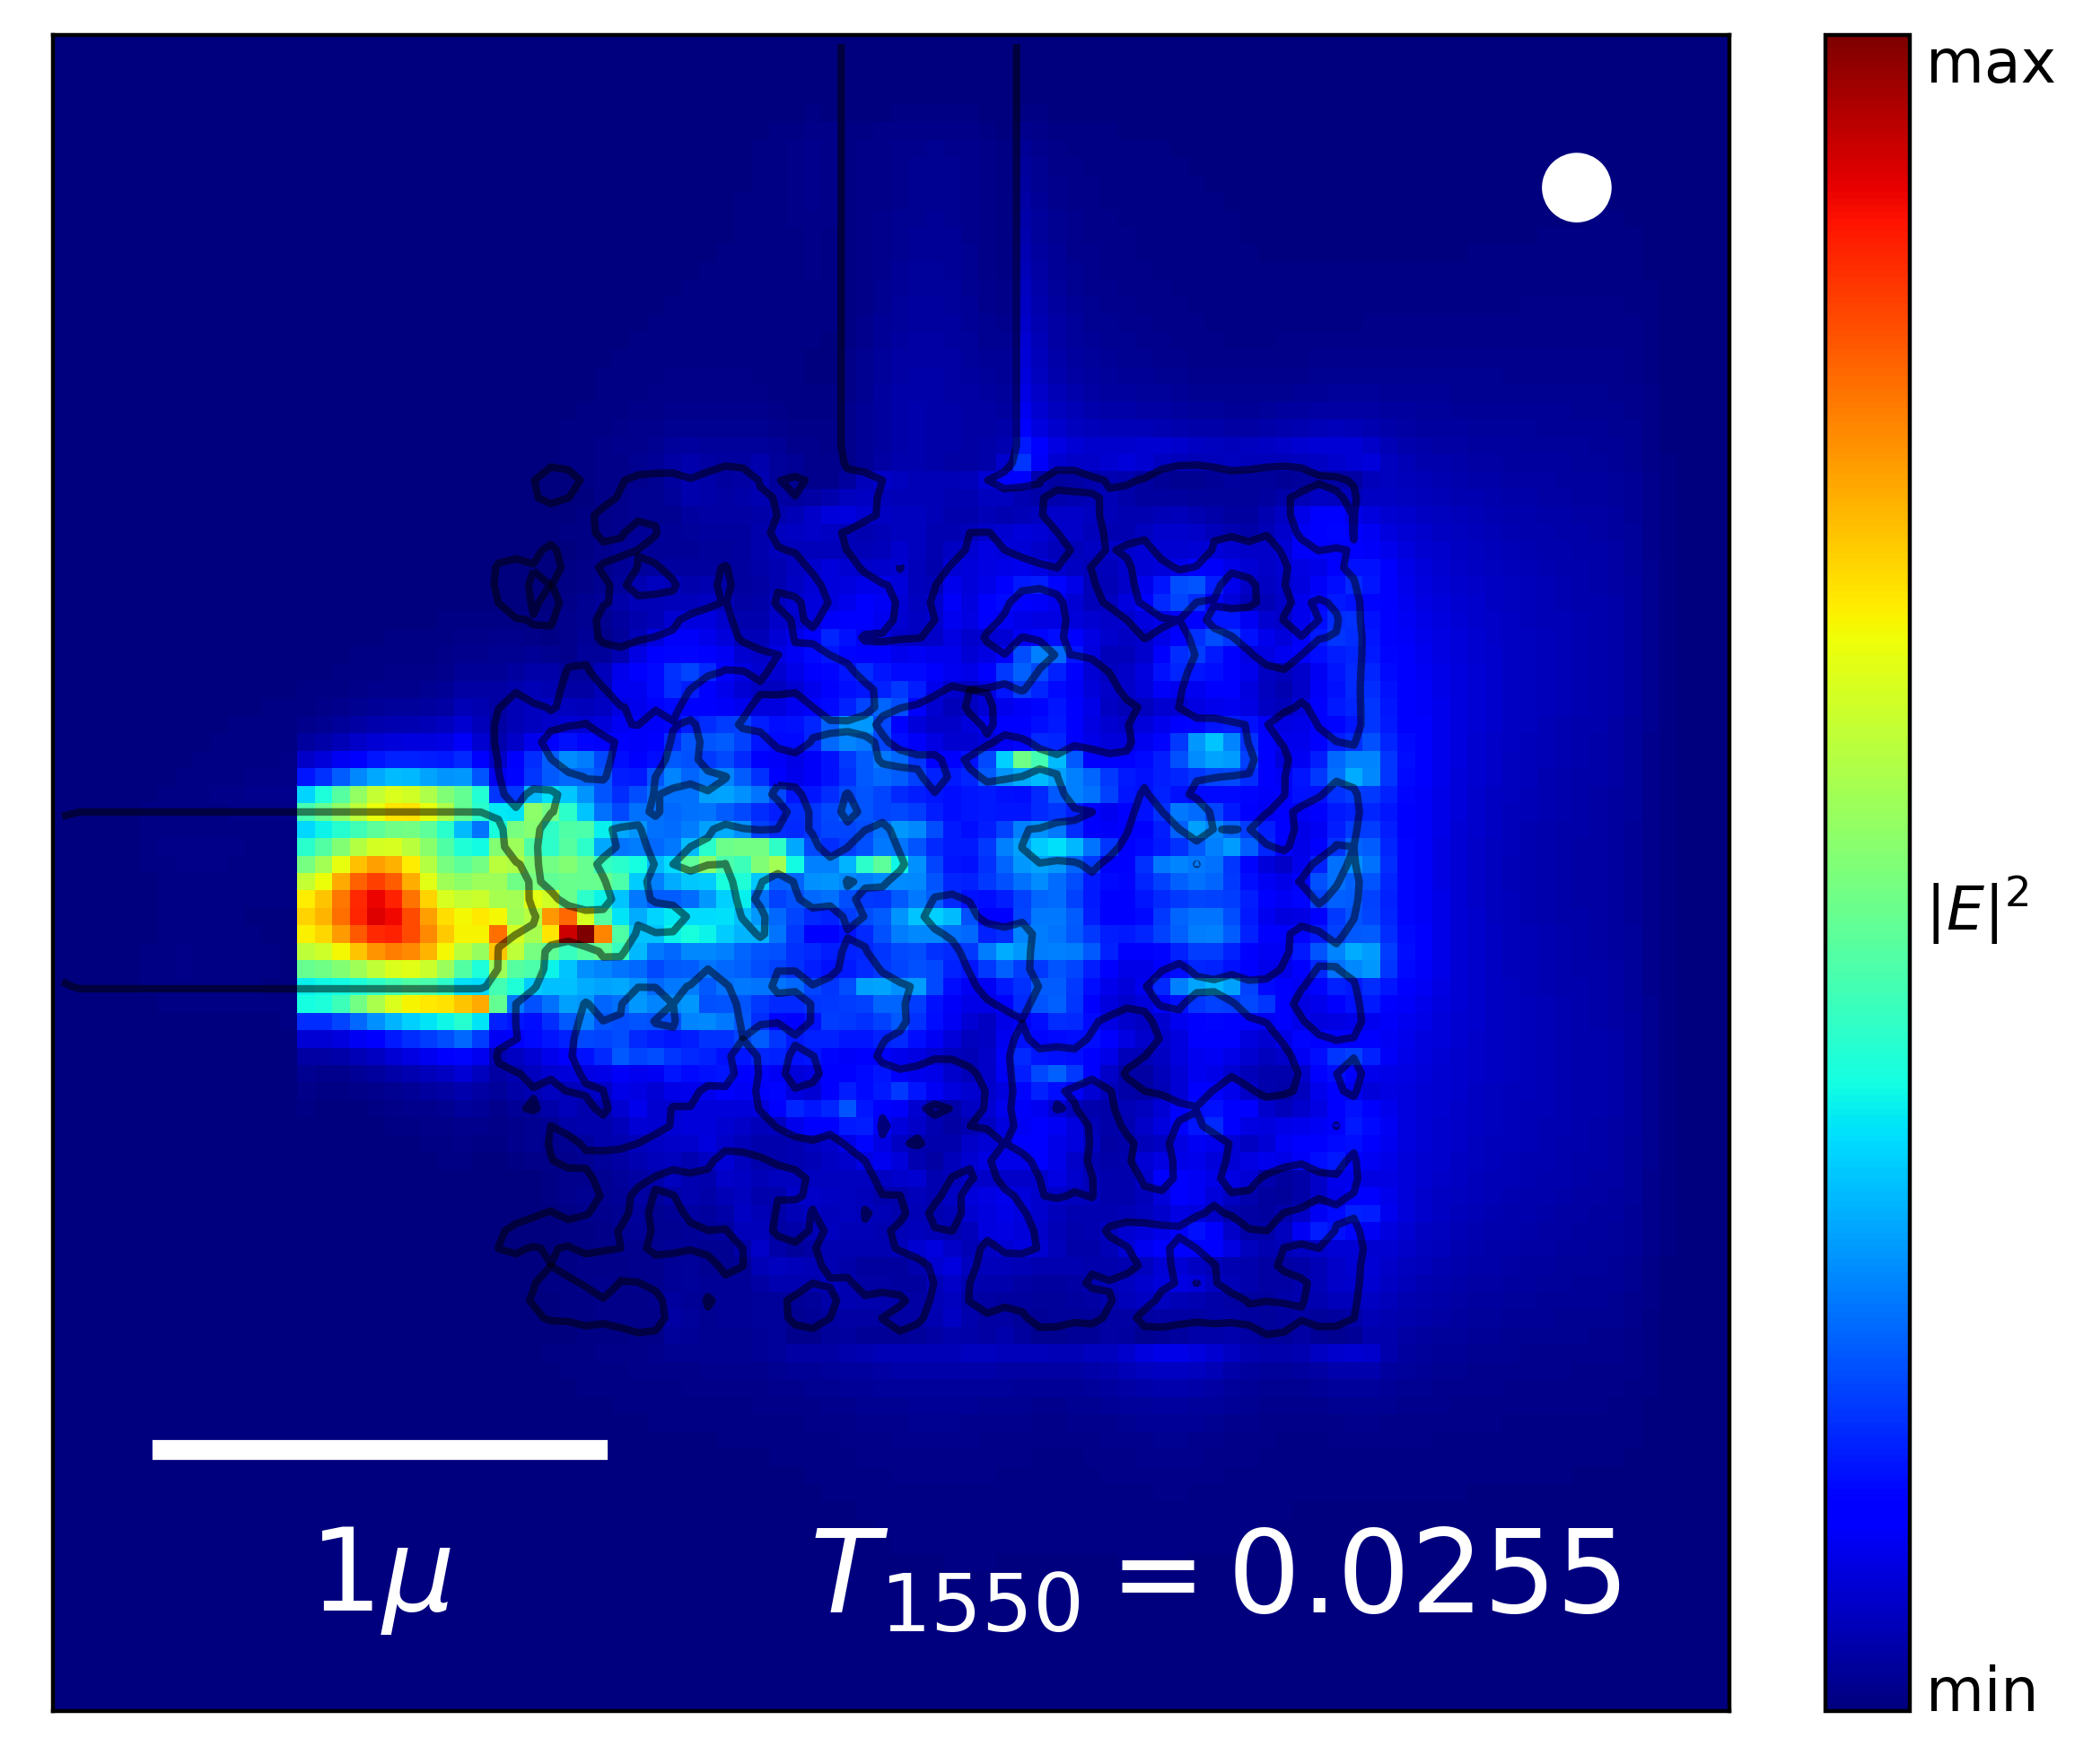
\includegraphics[width=0.33\textwidth]{image/results/bend/MMA/visualize_field_disc_256.png} &
      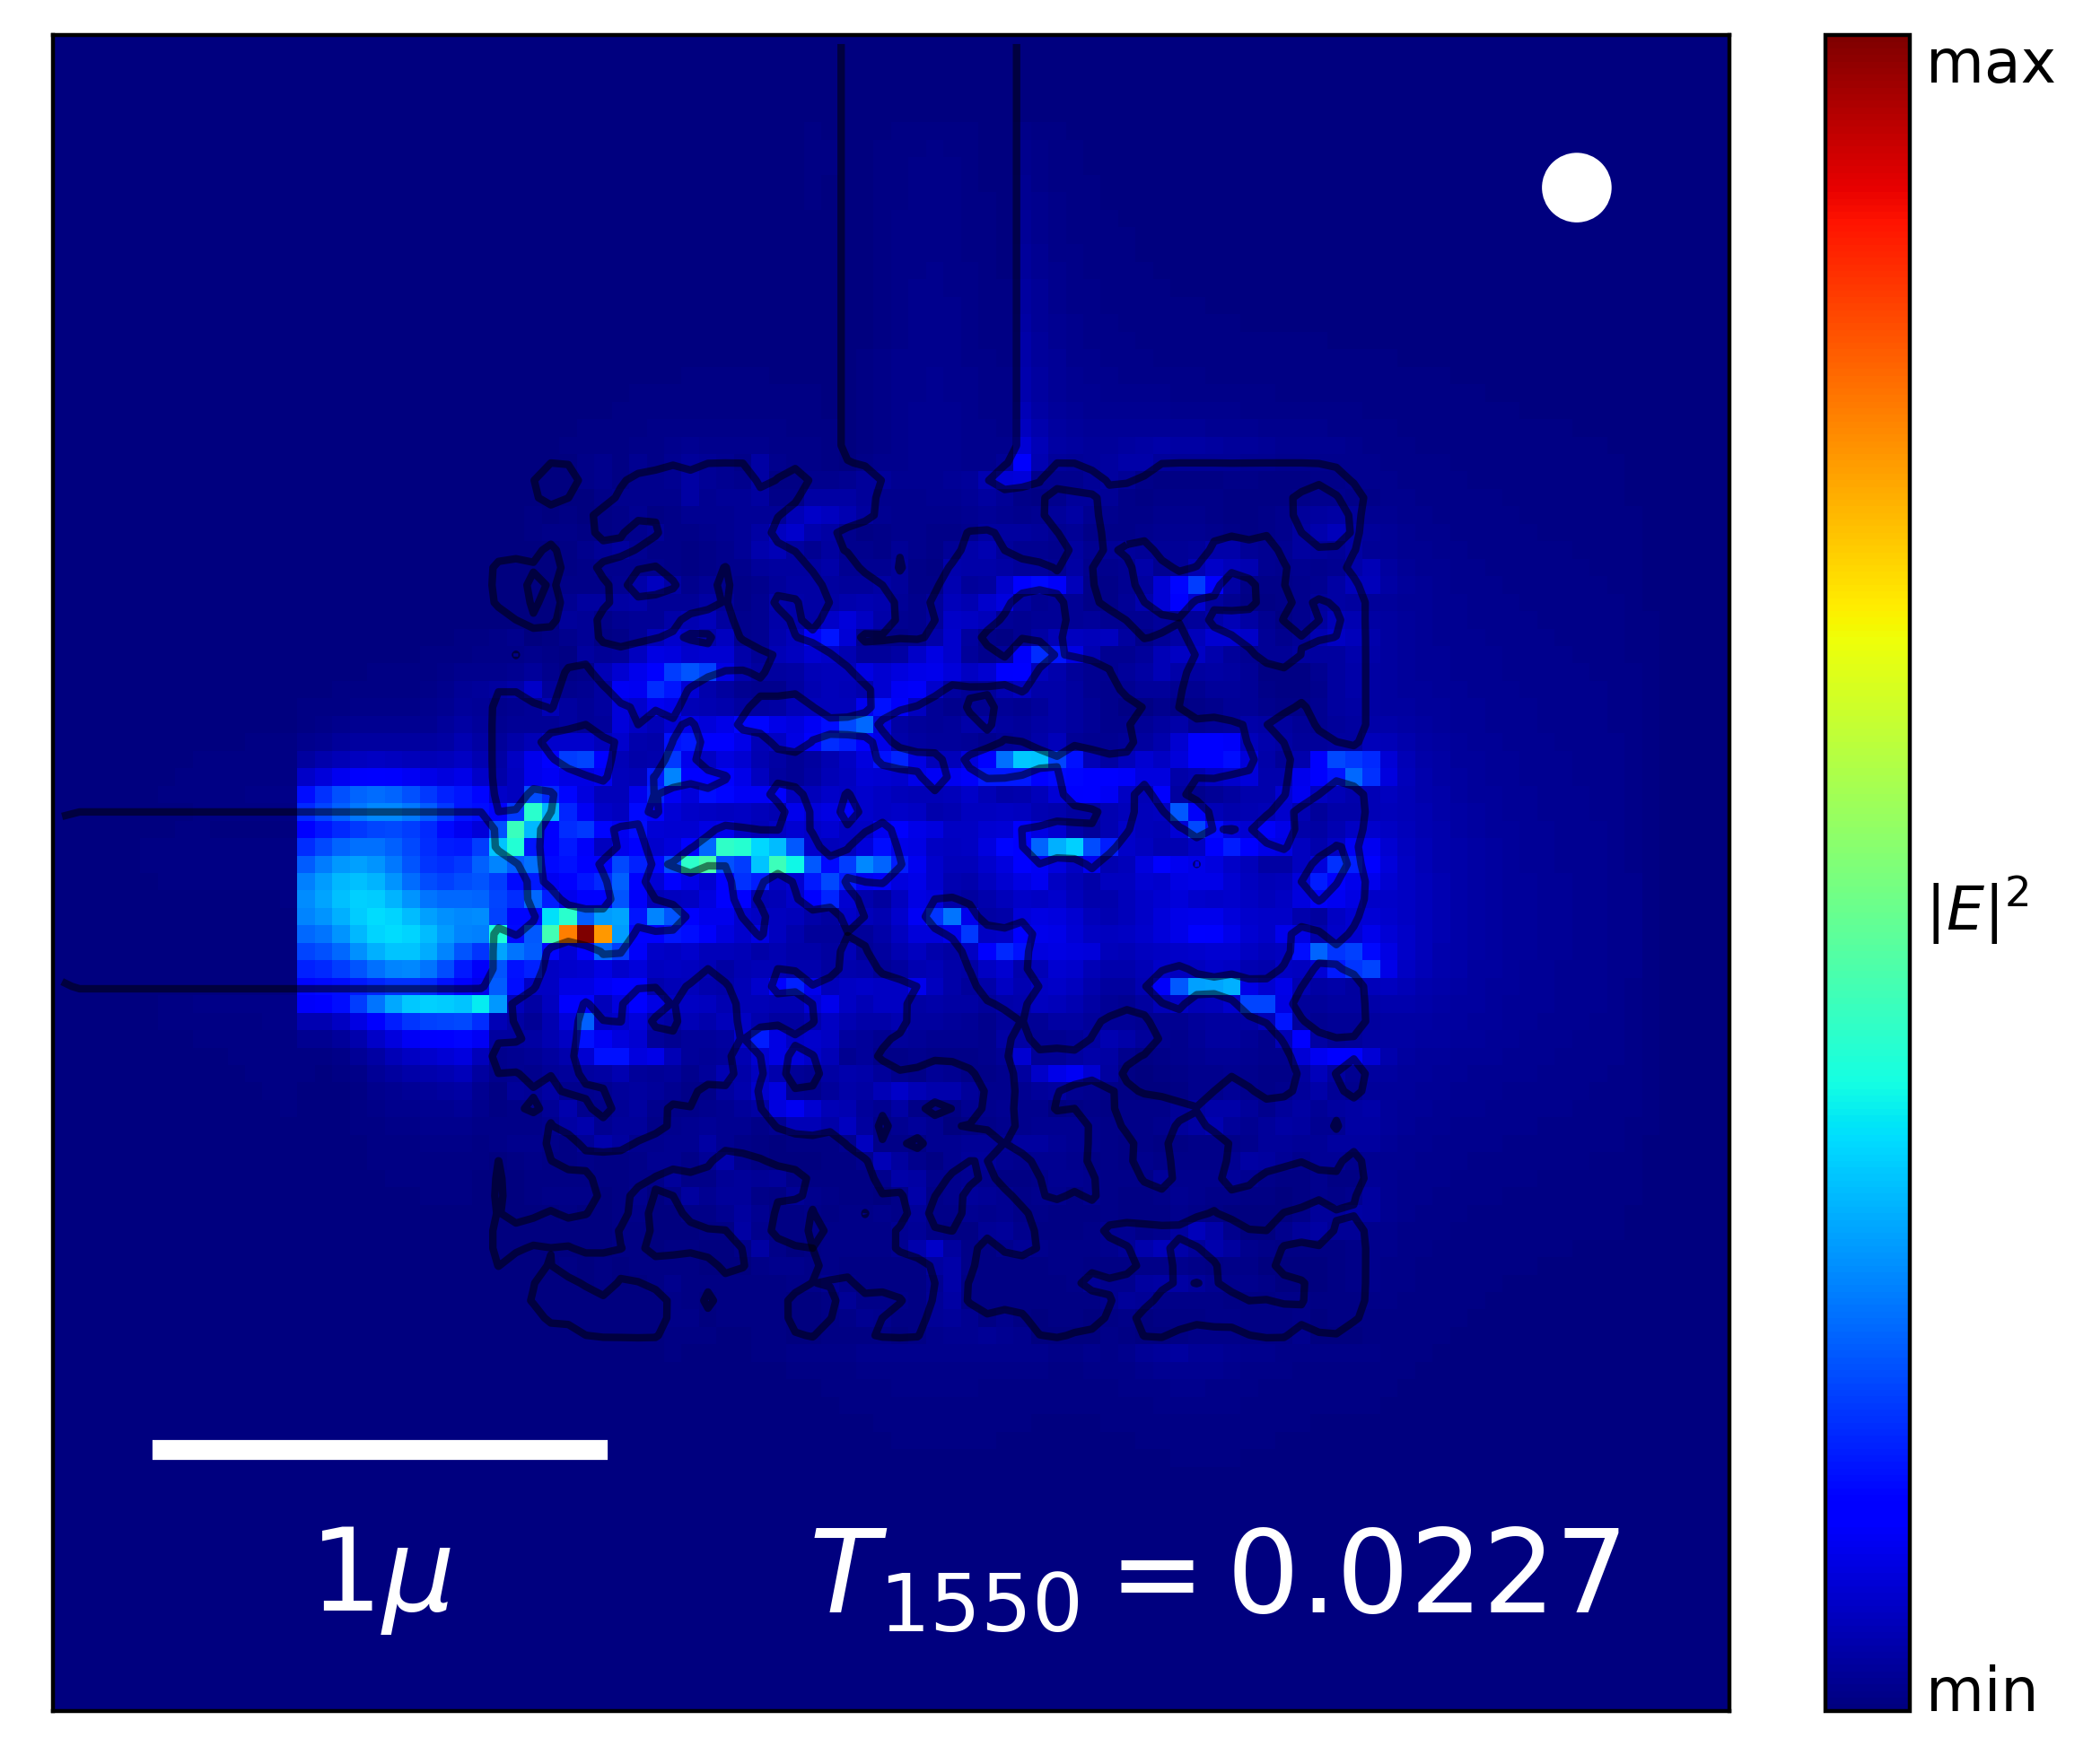
\includegraphics[width=0.33\textwidth]{image/results/bend/MMA/visualize_field_fab_256.png} \\
    \hline
      \multirow{2}{*}{512} &
      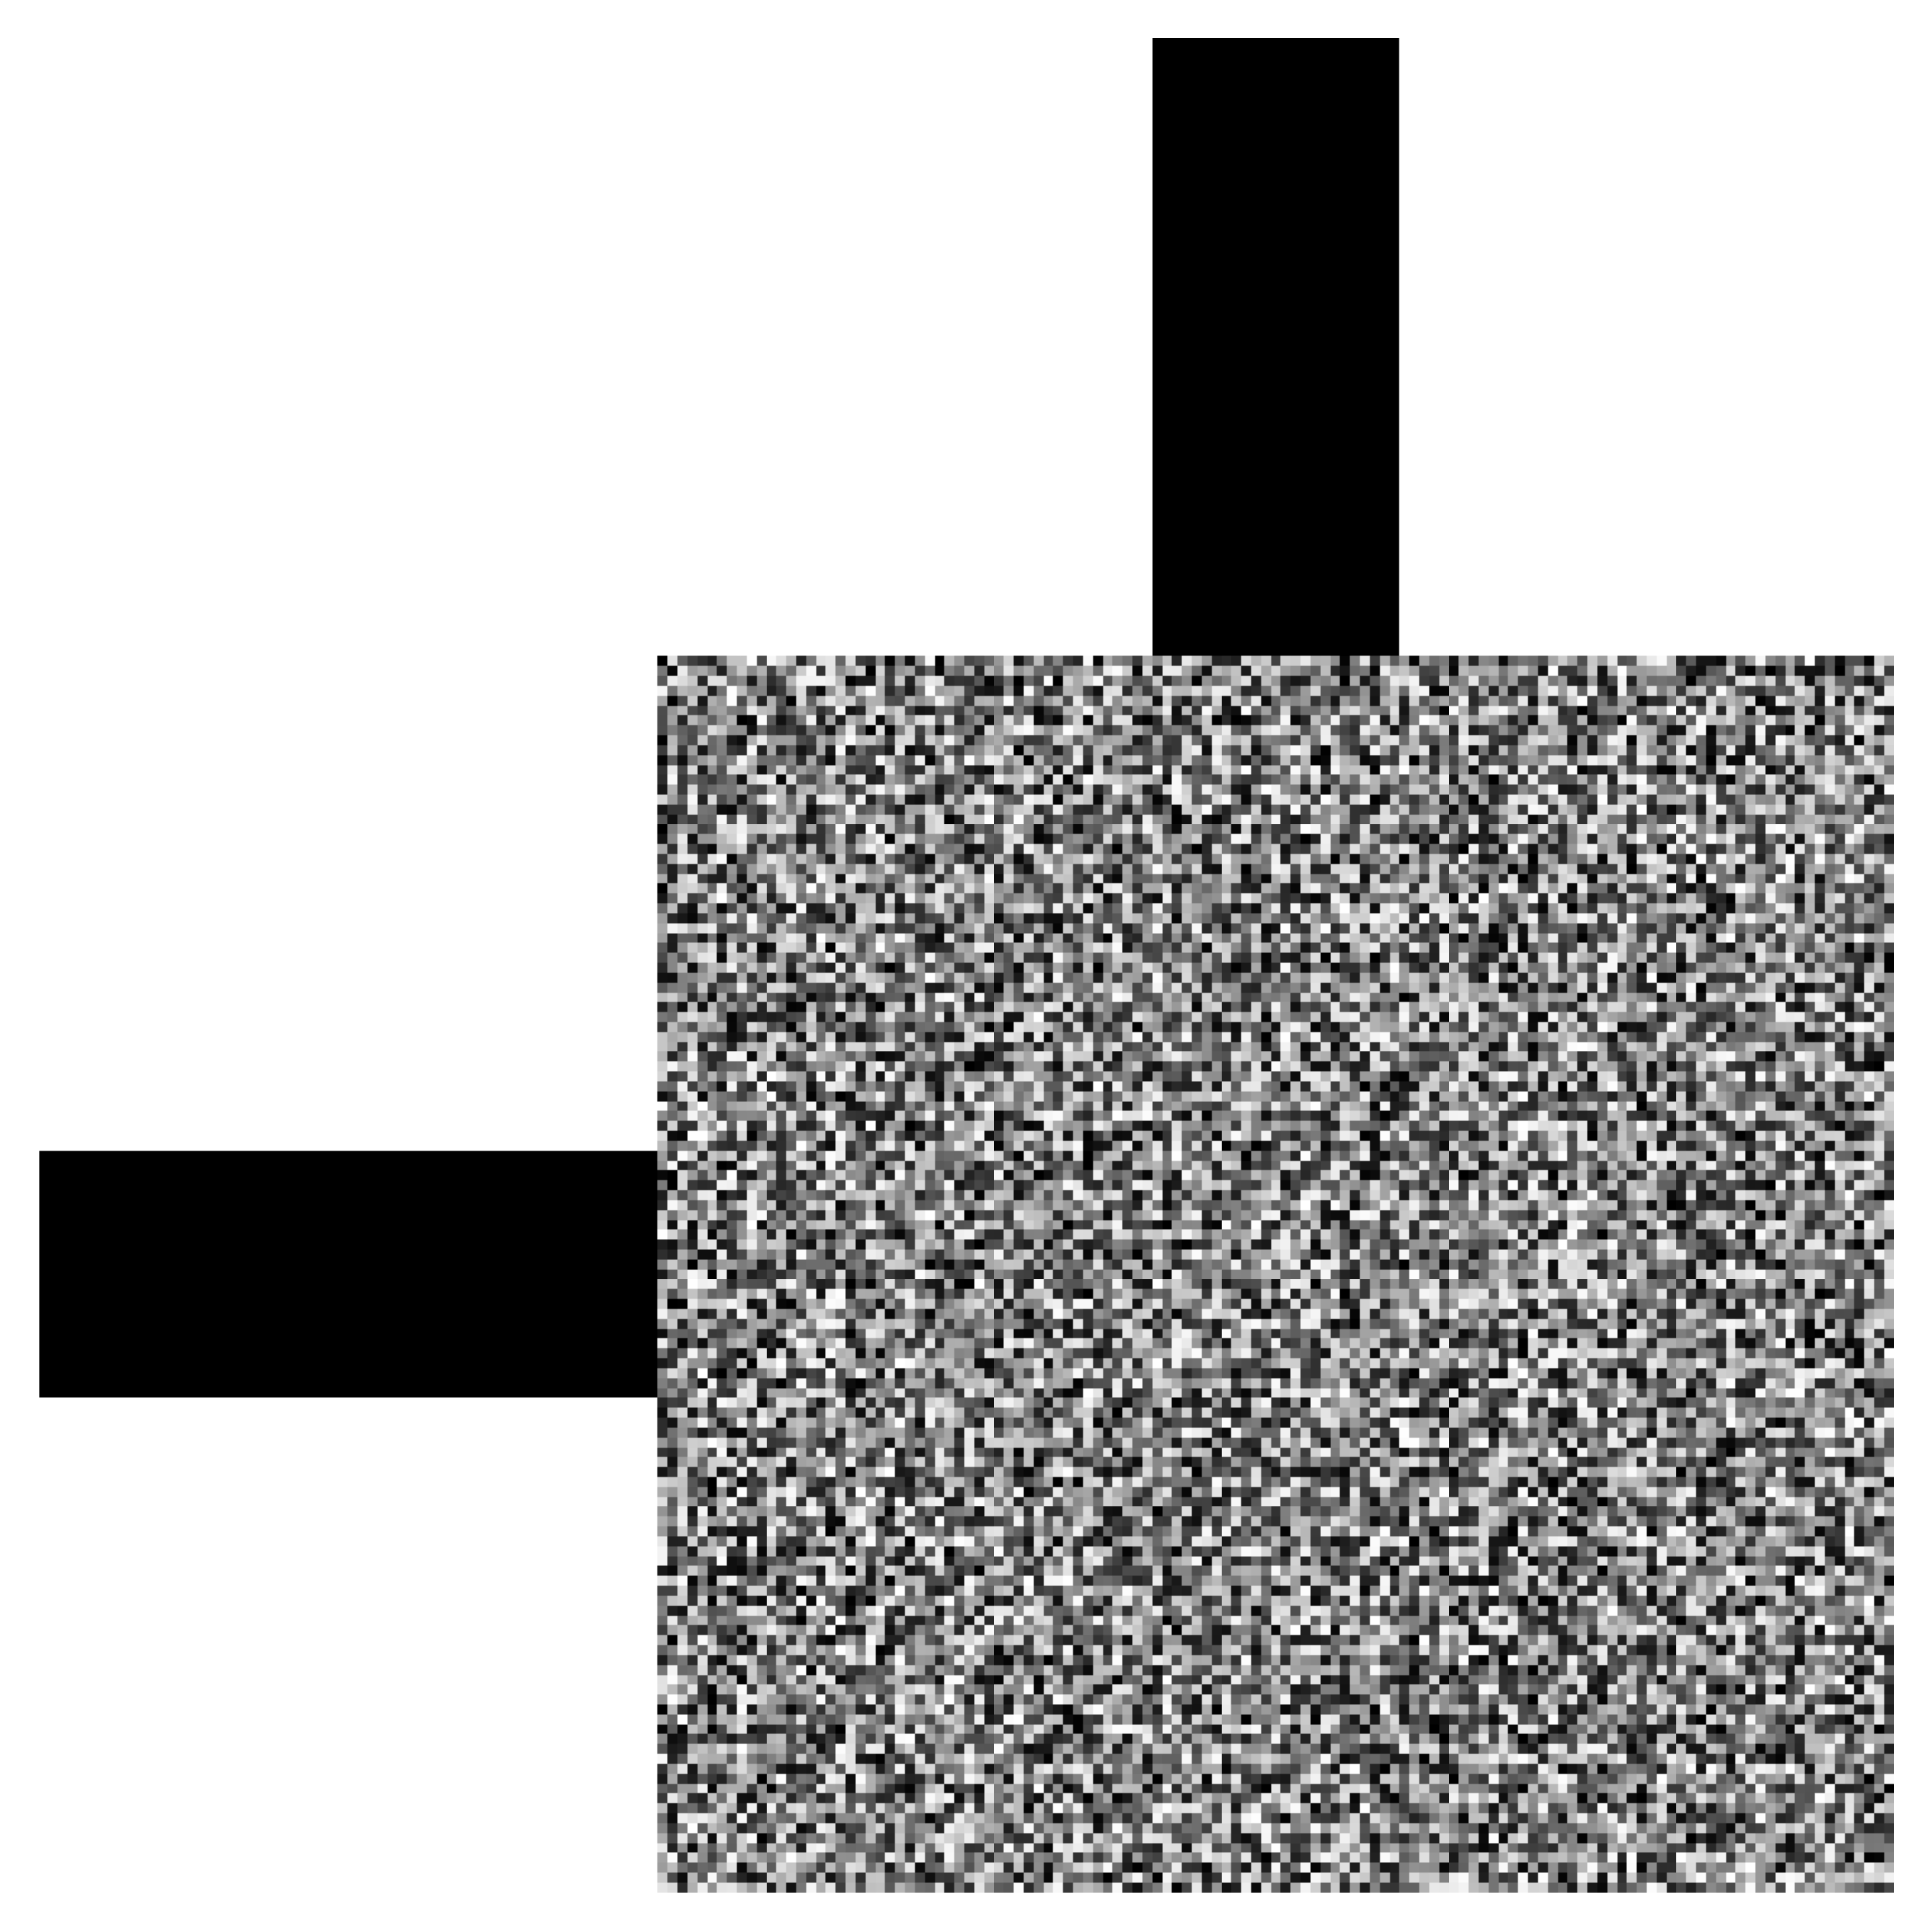
\includegraphics[width=0.20\textwidth]{image/results/bend/MMA/visualize_eps_cont_512.png} &
      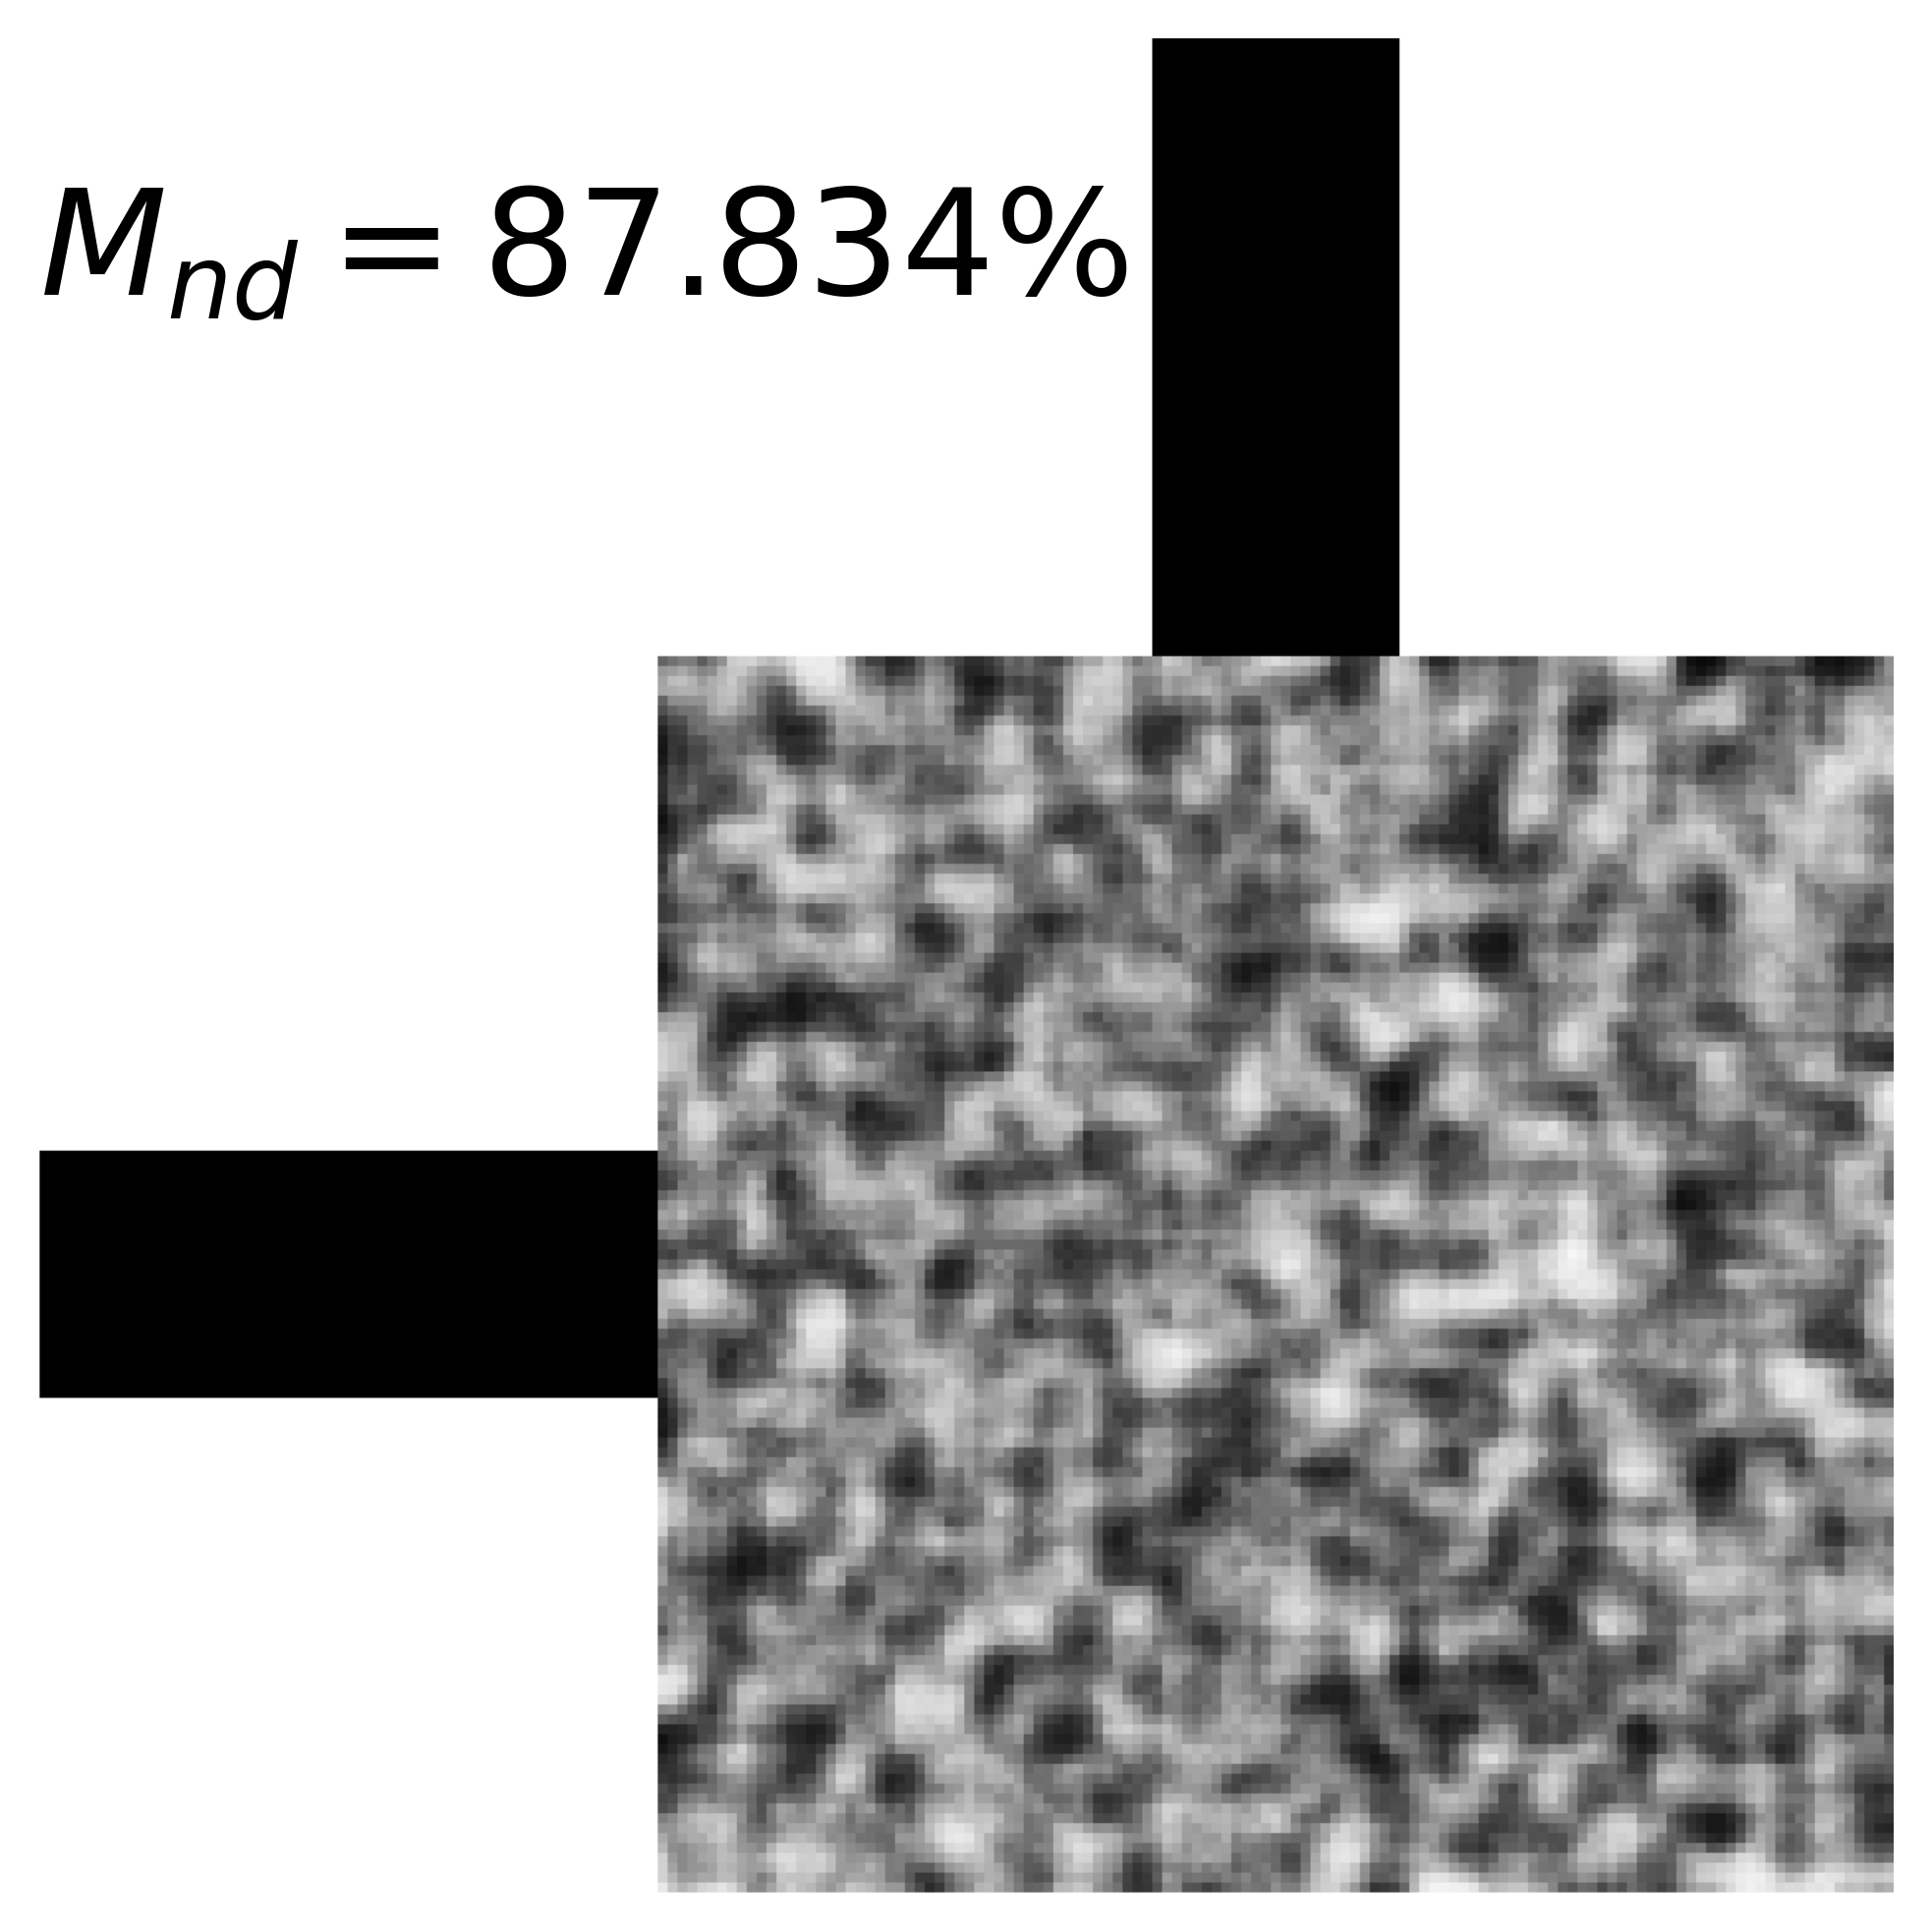
\includegraphics[width=0.20\textwidth]{image/results/bend/MMA/visualize_eps_disc_512.png} &
      \includegraphics[width=0.20\textwidth]{image/results/bend/MMA/visualize_eps_fab_512.png} \\
      \cline{2-4}
      &
      \includegraphics[width=0.33\textwidth]{image/results/bend/MMA/visualize_field_cont_512.png} &
      \includegraphics[width=0.33\textwidth]{image/results/bend/MMA/visualize_field_disc_512.png} &
      \includegraphics[width=0.33\textwidth]{image/results/bend/MMA/visualize_field_fab_512.png} \\
    \hline
    \end{tabular}
    \hspace*{-3cm}
    \caption{Resultados de optimizar el \emph{bend} usando MMA.}
    \label{tab:opt-MMA-bend}
\end{table}

% Bend - PSO
\begin{table}[ht]
    \centering
    \vspace*{-2.5cm}
    \hspace*{-3cm}
    \begin{tabular}{|c|c|c|c|}
    \hline 
    \emph{Seed} & Opt. continua & Opt. discreta &  Opt. de fabricación \\
    \hline
      \multirow{2}{*}{128} &
      \includegraphics[width=0.20\textwidth]{image/results/bend/PSO/visualize_eps_cont_128.png} &
      \includegraphics[width=0.20\textwidth]{image/results/bend/PSO/visualize_eps_disc_128.png} &
      \includegraphics[width=0.20\textwidth]{image/results/bend/PSO/visualize_eps_fab_128.png} \\
      \cline{2-4}
      &
      \includegraphics[width=0.33\textwidth]{image/results/bend/PSO/visualize_field_cont_128.png} &
      \includegraphics[width=0.33\textwidth]{image/results/bend/PSO/visualize_field_disc_128.png} &
      \includegraphics[width=0.33\textwidth]{image/results/bend/PSO/visualize_field_fab_128.png} \\
    \hline
      \multirow{2}{*}{256} &
      \includegraphics[width=0.20\textwidth]{image/results/bend/PSO/visualize_eps_cont_256.png} &
      \includegraphics[width=0.20\textwidth]{image/results/bend/PSO/visualize_eps_disc_256.png} &
      \includegraphics[width=0.20\textwidth]{image/results/bend/PSO/visualize_eps_fab_256.png} \\
      \cline{2-4}
      &
      \includegraphics[width=0.33\textwidth]{image/results/bend/PSO/visualize_field_cont_256.png} &
      \includegraphics[width=0.33\textwidth]{image/results/bend/PSO/visualize_field_disc_256.png} &
      \includegraphics[width=0.33\textwidth]{image/results/bend/PSO/visualize_field_fab_256.png} \\
    \hline
      \multirow{2}{*}{512} &
      \includegraphics[width=0.20\textwidth]{image/results/bend/PSO/visualize_eps_cont_512.png} &
      \includegraphics[width=0.20\textwidth]{image/results/bend/PSO/visualize_eps_disc_512.png} &
      \includegraphics[width=0.20\textwidth]{image/results/bend/PSO/visualize_eps_fab_512.png} \\
      \cline{2-4}
      &
      \includegraphics[width=0.33\textwidth]{image/results/bend/PSO/visualize_field_cont_512.png} &
      \includegraphics[width=0.33\textwidth]{image/results/bend/PSO/visualize_field_disc_512.png} &
      \includegraphics[width=0.33\textwidth]{image/results/bend/PSO/visualize_field_fab_512.png} \\
    \hline
    \end{tabular}
    \hspace*{-3cm}
    \caption{Resultados de optimizar el \emph{bend} usando G-PSO.}
    \label{tab:opt-PSO-bend}
\end{table}

% Bend - GA
\begin{table}[ht]
    \centering
    \vspace*{-2.5cm}
    \hspace*{-3cm}
    \begin{tabular}{|c|c|c|c|}
    \hline 
    \emph{Seed} & Opt. continua & Opt. discreta &  Opt. de fabricación \\
    \hline
      \multirow{2}{*}{128} &
      \includegraphics[width=0.20\textwidth]{image/results/bend/GA/visualize_eps_cont_128.png} &
      \includegraphics[width=0.20\textwidth]{image/results/bend/GA/visualize_eps_disc_128.png} &
      \includegraphics[width=0.20\textwidth]{image/results/bend/GA/visualize_eps_fab_128.png} \\
      \cline{2-4}
      &
      \includegraphics[width=0.33\textwidth]{image/results/bend/GA/visualize_field_cont_128.png} &
      \includegraphics[width=0.33\textwidth]{image/results/bend/GA/visualize_field_disc_128.png} &
      \includegraphics[width=0.33\textwidth]{image/results/bend/GA/visualize_field_fab_128.png} \\
    \hline
      \multirow{2}{*}{256} &
      \includegraphics[width=0.20\textwidth]{image/results/bend/GA/visualize_eps_cont_256.png} &
      \includegraphics[width=0.20\textwidth]{image/results/bend/GA/visualize_eps_disc_256.png} &
      \includegraphics[width=0.20\textwidth]{image/results/bend/GA/visualize_eps_fab_256.png} \\
      \cline{2-4}
      &
      \includegraphics[width=0.33\textwidth]{image/results/bend/GA/visualize_field_cont_256.png} &
      \includegraphics[width=0.33\textwidth]{image/results/bend/GA/visualize_field_disc_256.png} &
      \includegraphics[width=0.33\textwidth]{image/results/bend/GA/visualize_field_fab_256.png} \\
    \hline
      \multirow{2}{*}{512} &
      \includegraphics[width=0.20\textwidth]{image/results/bend/GA/visualize_eps_cont_512.png} &
      \includegraphics[width=0.20\textwidth]{image/results/bend/GA/visualize_eps_disc_512.png} &
      \includegraphics[width=0.20\textwidth]{image/results/bend/GA/visualize_eps_fab_512.png} \\
      \cline{2-4}
      &
      \includegraphics[width=0.33\textwidth]{image/results/bend/GA/visualize_field_cont_512.png} &
      \includegraphics[width=0.33\textwidth]{image/results/bend/GA/visualize_field_disc_512.png} &
      \includegraphics[width=0.33\textwidth]{image/results/bend/GA/visualize_field_fab_512.png} \\
    \hline
    \end{tabular}
    \hspace*{-3cm}
    \caption{Resultados de optimizar el \emph{bend} usando G-GA.}
    \label{tab:opt-GA-bend}
\end{table}
